% Template:     Informe/Reporte LaTeX
% Documento:    Archivo principal
% Versión:      6.6.0 (19/09/2019)
% Codificación: UTF-8
%
% Autor: Pablo Pizarro R.
%        Facultad de Ciencias Físicas y Matemáticas
%        Universidad de Chile
%        pablo@ppizarror.com
%
% Manual template: [https://latex.ppizarror.com/informe]
% Licencia MIT:    [https://opensource.org/licenses/MIT]

% CREACIÓN DEL DOCUMENTO
\documentclass[letterpaper,11pt]{article} % Articulo tamaño carta, 11pt
\usepackage[utf8]{inputenc} % Codificación UTF-8


% INFORMACIÓN DEL DOCUMENTO
\def\titulodelinforme {Apuntes Simulación Estocástica}
\def\temaatratar {MA4402 - Simulación Estocástica: Teoría y Laboratorio}

\def\autordeldocumento {}%{Camilo Carvajal Reyes}
\def\nombredelcurso {Simulación Estocástica: Teoría y Laboratorio}
\def\codigodelcurso {MA4402}

\def\nombreuniversidad {Departamento de Ingeniería Matemática}
\def\nombrefacultad {}
\def\departamentouniversidad {}
\def\imagendepartamento {dim}
\def\imagendepartamentoescala {0.2}
\def\localizacionuniversidad {}

% INTEGRANTES, PROFESORES Y FECHAS
\def\tablaintegrantes {
\begin{tabular}{ll}
	{}
	& \begin{tabular}[t]{l}
		{}
	\end{tabular} \\
	Profesor:
	%& \begin{tabular}[t]{l}
		Joaquín Fontbona
	%\end{tabular} \\
	%& \\
	\multicolumn{2}{l}{\today} \\
	\multicolumn{2}{l}{\localizacionuniversidad}
\end{tabular}}{
}

% CONFIGURACIONES
% Template:     Informe/Reporte LaTeX
% Documento:    Configuraciones del template
% Versión:      6.6.0 (19/09/2019)
% Codificación: UTF-8
%
% Autor: Pablo Pizarro R.
%        Facultad de Ciencias Físicas y Matemáticas
%        Universidad de Chile
%        pablo@ppizarror.com
%
% Manual template: [https://latex.ppizarror.com/informe]
% Licencia MIT:    [https://opensource.org/licenses/MIT]

% CONFIGURACIONES GENERALES
\def\addemptypagetwosides {false}  % Añade pag en blanco al imprimir a 2 caras
\def\defaultinterline {1.0}        % Interlineado por defecto [pt]
\def\defaultnewlinesize {11}       % Tamaño del salto de línea [pt]
\def\documentlang {en-NZ}          % Define el idioma del documento
\def\fontdocument {lmodern}        % Tipografía base, ver soportadas en manual
\def\fonttypewriter {tmodern}      % Tipografía de \texttt, ver manual online
\def\fonturl {tt}                  % Tipo de fuente url {tt,sf,rm,same}
\def\importtikz {false}            % Utilizar la librería tikz
\def\pointdecimal {true}           % N° decimales con punto en vez de coma
\def\predocpageromannumber {true}  % Pág. con número romano previo a inicio doc.
\def\predocpageromanupper {false}  % Páginas en número romano en mayúsculas
\def\predocresetpagenumber {true}  % Resetea número de la pag. tras el índice
\def\showlinenumbers {false}       % Muestra los números de línea del documento

% ESTILO PORTADA Y HEADER-FOOTER
\def\disablehfrightmark {false}    % Desactiva el rightmark del header-footer
\def\hfstyle {style1}              % Estilo header-footer (16 estilos)
\def\hfwidthcourse {0.35}          % Tamaño máximo del curso en header-footer
\def\hfwidthtitle {0.6}            % Tamaño máximo del título en header-footer
\def\hfwidthwrap {false}           % Activa el tamaño máximo en header-footer
\def\portraitstyle {style9}        % Estilo portada (20 estilos)

% CONFIGURACIÓN DE LAS LEYENDAS - CAPTION
\def\captionalignment {justified}  % Posición {centered,justified,left,right}
\def\captionlabelformat {simple}   % Formato leyenda {empty,simple,parens}
\def\captionlabelsep {colon}       % Sep. {none,colon,period,space,quad,newline}
\def\captionlessmarginimage {0.1}  % Margen sup/inf de fig. si no hay ley. [cm]
\def\captionlrmargin {2.0}         % Márgenes izq/der de la leyenda [cm]
\def\captionmarginmultimg {0.0}    % Margen izq/der leyendas múltiple img [cm]
\def\captionnumcode {arabic}       % N° código {arabic,alph,Alph,roman,Roman}
\def\captionnumequation {arabic}   % N° ecuaciones {arabic,alph,Alph,roman,Roman}
\def\captionnumfigure {arabic}     % N° figuras {arabic,alph,Alph,roman,Roman}
\def\captionnumsubfigure {alph}    % N° subfiguras {arabic,alph,Alph,roman,Roman}
\def\captionnumsubtable {alph}     % N° subtabla {arabic,alph,Alph,roman,Roman}
\def\captionnumtable {arabic}      % N° tabla {arabic,alph,Alph,roman,Roman}
\def\captiontbmarginfigure {9.35}  % Margen sup/inf de la leyenda en fig. [pt]
\def\captiontbmargintable {7.0}    % Margen sup/inf de la leyenda en tab. [pt]
\def\captiontextbold {false}       % Etiqueta (código,figura,tabla) en negrita
\def\captiontextsubnumbold {false} % N° subfigura/subtabla en negrita
\def\codecaptiontop {true}         % Leyenda arriba del código fuente
\def\figurecaptiontop {false}      % Leyenda arriba de las imágenes
\def\sectioncaptiondelimiter {.}   % Carácter delimitador n° objeto y sección
\def\showsectioncaptioncode {none} % N° sec. código {none,chap,(s/ss/sss/ssss)ec}
\def\showsectioncaptioneqn {none}  % N° sec. ecuación {none,chap,(s/ss/sss/ssss)ec}
\def\showsectioncaptionfig {none}  % N° sec. figuras {none,chap,(s/ss/sss/ssss)ec}
\def\showsectioncaptionmat {none}  % N° matemático {none,chap,(s/ss/sss/ssss)ec}
\def\showsectioncaptiontab {none}  % N° sec. tablas {none,chap,(s/ss/sss/ssss)ec}
\def\subcaptionlabelformat{parens} % Formato leyenda sub. {empty,simple,parens}
\def\subcaptionlabelsep {space}    % Sep. {none,colon,period,space,quad,newline}
\def\tablecaptiontop {true}        % Leyenda arriba de las tablas

% CONFIGURACIÓN DEL ÍNDICE
\def\addindextobookmarks {true}    % Añade el índice a los marcadores del pdf
\def\charafterobjectindex {.}      % Carácter después de n° figura,tabla,código
\def\charnumpageindex {.}          % Carácter número de página en índice
\def\indexdepth {4}                % Profundidad máxima del índice
\def\indexnewpagec {false}         % Nueva página en índice códigos fuente
\def\indexnewpagef {false}         % Nueva página en índice figuras
\def\indexnewpaget {false}         % Nueva página en índice tablas
\def\indexstyle {} %{ftc}              % Estilo índice {f:figura, t:tabla, c:código}
\def\indextitlemargin {11.4}       % Margen título índice \insertindextitle [pt]
\def\objectindexindent {false}     % Indenta la lista de objetos
\def\showappendixsecindex {false}  % Título de la sec. de anexos en el índice
\def\showindex {true}              % Muestra el índice
\def\showindexofcontents {true}    % Muestra la lista de contenidos

% ANEXO, CITAS, REFERENCIAS
\def\apaciterefsep {9}             % Separación entre refs. {apacite} [pt]
\def\appendixindepobjnum {true}    % Anexo usa n° objetos independientes
\def\bibtexrefsep {6}              % Separación entre refs. {bibtex} [pt]
\def\natbibnumbers {true}          % Forza el uso de números en la bibliografía
\def\natbibrefsep {6}              % Separación entre referencia {natbib} [pt]
\def\natbibrefstyle {ieeetr}       % Formato de ref. natbib {apa,ieeetr,etc...}
\def\natbibsquare {true}           % Usa [] o () en las numeraciones
\def\sectionappendixlastchar {.}   % Carácter entre n° de sec. anexo y título
\def\sectionrefenv {false}         % Las referencias se consideran como sección
\def\stylecitereferences {bibtex}  % Estilo cita/ref. {apacite,bibtex,natbib}
\def\twocolumnreferences {false}   % Referencias en dos columnas

% CONFIGURACIONES DE OBJETOS
\def\columnhspace {-0.4}           % Margen horizontal entre obj. \createcolumn
\def\columnsepwidth {2.1}          % Separación entre columnas [em]
\def\defaultimagefolder {img/}     % Carpeta raíz de las imágenes
\def\equationleftalign {false}     % Ecuaciones alineadas a la izquierda
\def\equationrestart {none}        % Reinicio n° {none,chap,(s/ss/sss/ssss)ec}
\def\footnotepagetoprule {false}   % Footnote en pag. tienen separador superior
\def\footnoterestart {none}        % N° footnote {none,chap,page,(s/ss/sss/ssss)ec}
\def\imagedefaultplacement {H}     % Posición por defecto de las imágenes
\def\marginalignbottom {-0.30}     % Margen inferior entorno align [cm]
\def\marginaligncaptbottom {0.05}  % Margen inferior entorno align caption[cm]
\def\marginaligncapttop {-0.60}    % Margen superior entorno align caption [cm]
\def\marginalignedbottom {-0.30}   % Margen inferior entorno aligned [cm]
\def\marginalignedcaptbottom {0.0} % Margen inferior entorno aligned caption[cm]
\def\marginalignedcapttop {-0.60}  % Margen superior entorno aligned caption[cm]
\def\marginalignedtop {-0.40}      % Margen superior entorno aligned [cm]
\def\marginaligntop {-0.40}        % Margen superior entorno align [cm]
\def\margineqncaptionbottom {0.0}  % Margen inferior caption ecuación [cm]
\def\margineqncaptiontop {-0.65}   % Margen superior caption ecuación [cm]
\def\marginequationbottom {-0.15}  % Margen inferior ecuaciones [cm]
\def\marginequationtop {0.0}       % Margen superior ecuaciones [cm]
\def\marginfloatimages {-13.0}     % Margen sup. fig. insertimageleft/right [pt]
\def\marginfootnote {10.0}         % Margen derecho footnote [pt]
\def\margingatherbottom {-0.20}    % Margen inferior entorno gather [cm]
\def\margingathercaptbottom {0.05} % Margen inferior entorno gather caption [cm]
\def\margingathercapttop {-0.77}   % Margen superior entorno gather [cm]
\def\margingatheredbottom {-0.10}  % Margen inf. entorno gathered [cm]
\def\margingatheredcaptbottom{0.0} % Margen inf. entorno gathered caption [cm]
\def\margingatheredcapttop {-0.77} % Margen superior entorno gathered [cm]
\def\margingatheredtop {-0.40}     % Margen superior entorno gathered [cm]
\def\margingathertop {-0.40}       % Margen superior entorno gather [cm]
\def\marginimagebottom {-0.15}     % Margen inferior figura [cm]
\def\marginimagemultright {0.50}   % Margen derecho imágenes múltiples [cm]
\def\marginimagemulttop {-0.30}    % Margen superior imágenes múltiples [cm]
\def\marginimagetop {0.0}          % Margen superior figuras [cm]
\def\numberedequation {true}       % Ecuaciones con \insert... numeradas
\def\sourcecodefontf {\ttfamily}   % Tipo de letra código fuente
\def\sourcecodefonts {\small}      % Tamaño letra código fuente
\def\sourcecodenumbersep {6}       % Separación entre número línea y código [pt]
\def\sourcecodetabsize {3}         % Tamaño tabulación código fuente
\def\tabledefaultplacement {H}     % Posición por defecto de las tablas
\def\tablepaddingh {0.85}          % Espaciado horizontal de celda de las tablas
\def\tablepaddingv {1.05}          % Espaciado vertical de celda de las tablas
\def\tikzdefaultplacement {H}      % Posición por defecto de las figuras tikz

% CONFIGURACIÓN DE LOS TÍTULOS
\def\anumsecaddtocounter {false}   % Insertar títulos anum. aumenta n° de sec
\def\fontsizessstitle{\normalsize} % Tamaño sub-sub-subtítulos
\def\fontsizesubsubtitle {\large}  % Tamaño sub-subtítulos
\def\fontsizesubtitle {\Large}     % Tamaño subtítulos
\def\fontsizetitle {\LARGE}        % Tamaño títulos
\def\fontsizetitlei {\LARGE}       % Tamaño títulos en el índice
\def\showdotaftersnum {true}       % Punto al final de n° (s/ss/sss/ssss)ection
\def\stylessstitle {\bfseries}     % Estilo sub-sub-subtítulos
\def\stylesubsubtitle {\bfseries}  % Estilo sub-subtítulos
\def\stylesubtitle {\bfseries}     % Estilo subtítulos
\def\styletitle {\bfseries}        % Estilo títulos
\def\styletitlei {\bfseries}       % Estilo títulos en el índice

% CONFIGURACIÓN DE LOS COLORES DEL DOCUMENTO
\def\captioncolor {black}          % Color de la leyenda (código,figura,tabla)
\def\captiontextcolor {black}      % Color de la leyenda
\def\colorpage {white}             % Color de la página
\def\highlightcolor {yellow}       % Color del subrayado con \hl
\def\indextitlecolor {black}       % Color de los títulos del índice
\def\linenumbercolor {gray}        % Color del n° de línea (\showlinenumbers)
\def\linkcolor {black}             % Color de los links del documento
\def\maintextcolor {black}         % Color principal del texto
\def\numcitecolor {black}          % Color del n° de las referencias o citas
\def\portraittitlecolor {black}    % Color de los títulos de la portada
\def\showborderonlinks {false}     % Color de un link por un recuadro de color
\def\sourcecodebgcolor {lgray}     % Color de fondo del código fuente
\def\ssstitlecolor {black}         % Color de los sub-sub-subtítulos
\def\subsubtitlecolor {black}      % Color de los sub-subtítulos
\def\subtitlecolor {black}         % Color de los subtítulos
\def\tablelinecolor {black}        % Color de las líneas de las tablas
\def\tablerowfirstcolor {none}     % Primer color de celda de las tablas
\def\tablerowsecondcolor {gray!20} % Segundo color de celda de las tablas
\def\titlecolor {black}            % Color de los títulos
\def\urlcolor {magenta}            % Color de los enlaces web (\href,\url)

% MÁRGENES DE PÁGINA
\def\firstpagemargintop {3.8}      % Margen superior página portada [cm]
\def\pagemarginbottom {2.7}        % Margen inferior página [cm]
\def\pagemarginleft {2.54}         % Margen izquierdo página [cm]
\def\pagemarginright {2.54}        % Margen derecho página [cm]
\def\pagemargintop {3.0}           % Margen superior página [cm]

% OPCIONES DEL PDF COMPILADO
\def\cfgbookmarksopenlevel {1}     % Nivel marcadores en pdf (1:secciones)
\def\cfgpdfbookmarkopen {true}     % Expande marcadores del nivel configurado
\def\cfgpdfcenterwindow {true}     % Centra ventana del lector al abrir el pdf
\def\cfgpdfcopyright {}            % Establece el copyright del documento
\def\cfgpdfdisplaydoctitle {true}  % Muestra título del informe en visor
\def\cfgpdffitwindow {false}       % Ajusta la ventana del lector tamaño pdf
\def\cfgpdfkeywords {}             % Palabras clave del pdf
\def\cfgpdfmenubar {true}          % Muestra el menú del lector
\def\cfgpdfpagemode {OneColumn}    % Modo de página {OneColumn,SinglePage}
\def\cfgpdfpageview {FitH}         % {Fit,FitH,FitV,FitR,FitB,FitBH,FitBV}
\def\cfgpdfsecnumbookmarks {true}  % Número de la sec. en marcadores del pdf
\def\cfgpdftoolbar {true}          % Muestra barra de herramientas lector pdf
\def\cfgshowbookmarkmenu {false}   % Muestra menú marcadores al abrir el pdf
\def\pdfcompilecompression {9}     % Factor de compresión del pdf (0-9)
\def\pdfcompileobjcompression {2}  % Nivel compresión objetos del pdf (0-3)
\def\pdfcompileversion {7}         % Versión mínima del pdf compilado

% NOMBRE DE OBJETOS
\def\nameabstract {Resumen}  % Nombre del resumen-abstract
\def\nameappendixsection {Appendix}     % Nombre de los anexos
\def\namemathcol {Corolario}          % Nombre de los colorarios
\def\namemathdefn {Definición}        % Nombre de las definiciones
\def\namemathej {Ejemplo}             % Nombre de los ejemplos
\def\namemathlem {Lema}               % Nombre de los lemas
\def\namemathobs {Observación}        % Nombre de las observaciones
\def\namemathprp {Proposición}        % Nombre de las proposiciones
\def\namemaththeorem {Teorema}        % Nombre de los teoremas
\def\nameportraitpage {Front Page}       % Etiqueta página de la portada
\def\namereferences {Referencias}     % Nombre de la sección de referencias
\def\nomchapter {Chapter}            % Nombre de los capítulos
\def\nomltappendixsection {Anexo}     % Etiqueta sección en anexo/apéndices
\def\nomltcont {Indice} % Nombre del índice de contenidos
\def\nomltfigure {Indice de figuras}  % Nombre de la lista de figuras
\def\nomltsrc {Indice of códigos}     % Nombre de la lista de código
\def\nomlttable {Indice of tablas}    % Nombre de la lista de tablas
\def\nomltwfigure {Figura}            % Etiqueta leyenda de las figuras
\def\nomltwsrc {Código}               % Etiqueta leyenda del código fuente
\def\nomltwtable {Tabla}              % Etiqueta leyenda de las tablas
\def\nomnpageof { de }                % Etiqueta página # de #


% IMPORTACIÓN DE LIBRERÍAS
% Template:     Informe/Reporte LaTeX
% Documento:    Importación de librerías
% Versión:      6.6.0 (19/09/2019)
% Codificación: UTF-8
%
% Autor: Pablo Pizarro R.
%        Facultad de Ciencias Físicas y Matemáticas
%        Universidad de Chile
%        pablo@ppizarror.com
%
% Manual template: [https://latex.ppizarror.com/informe]
% Licencia MIT:    [https://opensource.org/licenses/MIT]

\usepackage[spanish,es-nosectiondot,es-lcroman,es-noquoting]{babel}
\usepackage{ifthen}
\newcommand{\throwbadconfig}[4][]{
	\ifthenelse{\equal{#1}{noheader}}{
		\errmessage{LaTeX Warning: #4}
	}{
		\ifthenelse{\equal{#1}{noheader-nostop}}{
			\errmessage{LaTeX Warning: #4}
		}{
			\errmessage{LaTeX Warning: #2 \noexpand #3=#3. Valores esperados: #4}
		}
	}
	\ifthenelse{\equal{#1}{nostop}}{}{
		\ifthenelse{\equal{#1}{noheader-nostop}}{}{
			\stop
		}
	}
}
\ifthenelse{\equal{\equationleftalign}{true}}{
	\usepackage[fleqn]{amsmath}
}{
	\usepackage{amsmath}
}
\let\counterwithout\relax
\let\counterwithin\relax
\let\RE\Re
\let\IM\Im
\usepackage{amssymb}
\usepackage{amsthm}
\usepackage{array}
\usepackage{bigstrut}
\usepackage{bm}
\usepackage{booktabs}
\usepackage{caption}
\usepackage{changepage}
\usepackage{chngcntr}
\usepackage{color}
\usepackage{datetime}
\usepackage{floatpag}
\usepackage{floatrow}
\usepackage{framed}
\usepackage{gensymb}
\usepackage{geometry}
\usepackage{graphicx}
\usepackage{lipsum}
\usepackage{listings}
\usepackage{listingsutf8}
\usepackage{longtable}
\usepackage{mathtools}
\usepackage{multicol}
\usepackage{needspace}
\usepackage{pdflscape}
\usepackage{pdfpages}
\usepackage{physics}
\usepackage{rotating}
\usepackage{sectsty}
\usepackage{selinput}
\usepackage{setspace}
\usepackage{soul}
\usepackage{subfig}
\usepackage{textcomp}
\usepackage{url}
\usepackage{wasysym}
\usepackage{wrapfig}
\usepackage{xspace}
\usepackage[makeroom]{cancel}
\usepackage[inline]{enumitem}
\usepackage[subfigure,titles]{tocloft}
\usepackage[figure,table,lstlisting]{totalcount}
\usepackage[normalem]{ulem}
\usepackage[dvipsnames,table,usenames]{xcolor}
\ifthenelse{\equal{\footnotepagetoprule}{true}}{
\usepackage[bottom,hang]{footmisc}
}{
	\usepackage[bottom,norule,hang]{footmisc}
}
\ifthenelse{\equal{\showdotaftersnum}{true}}{
	\usepackage{secdot}
	\sectiondot{subsection}
	\sectiondot{subsubsection}}{
}
\usepackage[pdfencoding=auto,psdextra]{hyperref}
\ifthenelse{\equal{\stylecitereferences}{natbib}}{
	\ifthenelse{\equal{\natbibrefstyle}{apa}}{
		\ifthenelse{\equal{\natbibsquare}{true}}{
			\usepackage[square]{natbib}
		}{
			\usepackage[round]{natbib}
		}
	}{
	\ifthenelse{\equal{\natbibrefstyle}{ieeetr}}{
		\ifthenelse{\equal{\natbibsquare}{true}}{
			\usepackage[square,numbers]{natbib}
		}{
			\usepackage[round,numbers]{natbib}
		}
	}{
	\ifthenelse{\equal{\natbibrefstyle}{unsrt}}{
		\ifthenelse{\equal{\natbibsquare}{true}}{
			\usepackage[square,numbers]{natbib}
		}{
			\usepackage[round,numbers]{natbib}
		}
	}{
	\ifthenelse{\equal{\natbibrefstyle}{abbrvnat}}{
		\ifthenelse{\equal{\natbibsquare}{true}}{
			\usepackage[square,numbers]{natbib}
		}{
			\usepackage[round,numbers]{natbib}
		}
	}{
		\ifthenelse{\equal{\natbibnumbers}{true}}{
			\ifthenelse{\equal{\natbibsquare}{true}}{
				\usepackage[square,numbers]{natbib}
			}{
				\usepackage[round,numbers]{natbib}
			}
		}{
			\ifthenelse{\equal{\natbibsquare}{true}}{
				\usepackage[square]{natbib}
			}{
				\usepackage[round]{natbib}
			}
		}
	}}}}
	\usepackage[nottoc,notlof,notlot]{tocbibind}
}{
\ifthenelse{\equal{\stylecitereferences}{apacite}}{
		\usepackage{apacite}
		\usepackage[nottoc,notlof,notlot]{tocbibind}
	}{
\ifthenelse{\equal{\stylecitereferences}{bibtex}}{
		}{}
	}
}
\ifthenelse{\equal{\showappendixsecindex}{true}}{
	\usepackage[toc]{appendix}
}{
	\usepackage{appendix}
}
\ifthenelse{\equal{\importtikz}{true}}{
	\usepackage{tikz}}{
}
\ifthenelse{\equal{\hfstyle}{style11}}{
	\usepackage{lastpage}}{}
\ifthenelse{\equal{\hfstyle}{style12}}{
	\usepackage{lastpage}}{}
\ifthenelse{\equal{\hfstyle}{style13}}{
	\usepackage{lastpage}}{}
\ifthenelse{\equal{\hfstyle}{style14}}{
	\usepackage{lastpage}}{
}
\usepackage{bookmark}
\usepackage{fancyhdr}
\usepackage{float}
\usepackage{hyperxmp}
\usepackage{multirow}
\usepackage{notoccite}
\usepackage{titlesec}
\ifthenelse{\equal{\fontdocument}{lmodern}}{
	\usepackage{lmodern}
}{
\ifthenelse{\equal{\fontdocument}{arial}}{
	\usepackage{helvet}
	\renewcommand{\familydefault}{\sfdefault}
}{
\ifthenelse{\equal{\fontdocument}{arial2}}{
	\usepackage{arial}
}{
\ifthenelse{\equal{\fontdocument}{times}}{
	\usepackage{mathptmx}
}{
\ifthenelse{\equal{\fontdocument}{helvet}}{
	\usepackage{helvet}
}{
\ifthenelse{\equal{\fontdocument}{alegreyasans}}{
	\usepackage[sfdefault]{AlegreyaSans}
	\renewcommand*\oldstylenums[1]{{\AlegreyaSansOsF #1}}
}{
\ifthenelse{\equal{\fontdocument}{mathpazo}}{
	\usepackage{mathpazo}
}{
\ifthenelse{\equal{\fontdocument}{accantis}}{
	\usepackage{accanthis}
}{
\ifthenelse{\equal{\fontdocument}{alegreya}}{
	\usepackage{Alegreya}
	\renewcommand*\oldstylenums[1]{{\AlegreyaOsF #1}}
}{
\ifthenelse{\equal{\fontdocument}{algolrevived}}{
	\usepackage{algolrevived}
}{
\ifthenelse{\equal{\fontdocument}{antiqua}}{
	\usepackage{antiqua}
}{
\ifthenelse{\equal{\fontdocument}{antpolt}}{
	\usepackage{antpolt}
}{
\ifthenelse{\equal{\fontdocument}{antpoltlight}}{
	\usepackage[light]{antpolt}
}{
\ifthenelse{\equal{\fontdocument}{anttor}}{
	\usepackage[math]{anttor}
}{
\ifthenelse{\equal{\fontdocument}{anttorcondensed}}{
	\usepackage[condensed,math]{anttor}
}{
\ifthenelse{\equal{\fontdocument}{anttorlight}}{
	\usepackage[light,math]{anttor}
}{
\ifthenelse{\equal{\fontdocument}{anttorlightcondensed}}{
	\usepackage[light,condensed,math]{anttor}
}{
\ifthenelse{\equal{\fontdocument}{arev}}{
	\usepackage{arev}
}{
\ifthenelse{\equal{\fontdocument}{arimo}}{
	\usepackage[sfdefault]{arimo}
	\renewcommand*\familydefault{\sfdefault}
}{
\ifthenelse{\equal{\fontdocument}{aurical}}{
	\usepackage{aurical}
}{
\ifthenelse{\equal{\fontdocument}{avant}}{
	\usepackage{avant}
}{
\ifthenelse{\equal{\fontdocument}{baskervald}}{
	\usepackage{baskervald}
}{
\ifthenelse{\equal{\fontdocument}{berasans}}{
	\usepackage[scaled]{berasans}
	\renewcommand*\familydefault{\sfdefault}
}{
\ifthenelse{\equal{\fontdocument}{beraserif}}{
	\usepackage{bera}
}{
\ifthenelse{\equal{\fontdocument}{biolinum}}{
	\usepackage{libertine}
	\renewcommand*\familydefault{\sfdefault}
}{
\ifthenelse{\equal{\fontdocument}{cabin}}{
	\usepackage[sfdefault]{cabin}
	\renewcommand*\familydefault{\sfdefault}
}{
\ifthenelse{\equal{\fontdocument}{cabincondensed}}{
	\usepackage[sfdefault,condensed]{cabin}
	\renewcommand*\familydefault{\sfdefault}
}{
\ifthenelse{\equal{\fontdocument}{cantarell}}{
	\usepackage[default]{cantarell}
}{
\ifthenelse{\equal{\fontdocument}{caladea}}{
	\usepackage{caladea}
}{
\ifthenelse{\equal{\fontdocument}{carlito}}{
	\usepackage[sfdefault]{carlito}
	\renewcommand*\familydefault{\sfdefault}
}{
\ifthenelse{\equal{\fontdocument}{chivolight}}{
	\usepackage[familydefault,light]{Chivo}
}{
\ifthenelse{\equal{\fontdocument}{chivoregular}}{
	\usepackage[familydefault,regular]{Chivo}
}{
\ifthenelse{\equal{\fontdocument}{clearsans}}{
	\usepackage[sfdefault]{ClearSans}
	\renewcommand*\familydefault{\sfdefault}
}{
\ifthenelse{\equal{\fontdocument}{comfortaa}}{
	\usepackage[default]{comfortaa}
}{
\ifthenelse{\equal{\fontdocument}{comicneue}}{
	\usepackage[default]{comicneue}
}{
\ifthenelse{\equal{\fontdocument}{comicneueangular}}{
	\usepackage[default,angular]{comicneue}
}{
\ifthenelse{\equal{\fontdocument}{crimson}}{
	\usepackage{crimson}
}{
\ifthenelse{\equal{\fontdocument}{cyklop}}{
	\usepackage{cyklop}
}{
\ifthenelse{\equal{\fontdocument}{dejavusans}}{
	\usepackage{DejaVuSans}
	\renewcommand*\familydefault{\sfdefault}
}{
\ifthenelse{\equal{\fontdocument}{dejavusanscondensed}}{
	\usepackage{DejaVuSansCondensed}
	\renewcommand*\familydefault{\sfdefault}
}{
\ifthenelse{\equal{\fontdocument}{droidsans}}{
	\usepackage[defaultsans]{droidsans}
	\renewcommand*\familydefault{\sfdefault}
}{
\ifthenelse{\equal{\fontdocument}{fetamont}}{
	\usepackage{fetamont}
	\renewcommand*\familydefault{\sfdefault}
}{
\ifthenelse{\equal{\fontdocument}{firasans}}{
	\usepackage[sfdefault]{FiraSans}
	\renewcommand*\familydefault{\sfdefault}
}{
\ifthenelse{\equal{\fontdocument}{iwona}}{
	\usepackage[math]{iwona}
}{
\ifthenelse{\equal{\fontdocument}{iwonacondensed}}{
	\usepackage[math]{iwona}
}{
\ifthenelse{\equal{\fontdocument}{iwonalight}}{
	\usepackage[light,math]{iwona}
}{
\ifthenelse{\equal{\fontdocument}{iwonalightcondensed}}{
	\usepackage[light,condensed,math]{iwona}
}{
\ifthenelse{\equal{\fontdocument}{kurier}}{
	\usepackage[math]{kurier}
}{
\ifthenelse{\equal{\fontdocument}{kuriercondensed}}{
	\usepackage[condensed,math]{kurier}
}{
\ifthenelse{\equal{\fontdocument}{kurierlight}}{
	\usepackage[light,math]{kurier}
}{
\ifthenelse{\equal{\fontdocument}{kurierlightcondensed}}{
	\usepackage[light,condensed,math]{kurier}
}{
\ifthenelse{\equal{\fontdocument}{lato}}{
	\usepackage[default]{lato}
}{
\ifthenelse{\equal{\fontdocument}{libris}}{
	\usepackage{libris}
	\renewcommand*\familydefault{\sfdefault}
}{
\ifthenelse{\equal{\fontdocument}{lxfonts}}{
	\usepackage{lxfonts}
}{
\ifthenelse{\equal{\fontdocument}{merriweather}}{
	\usepackage[sfdefault]{merriweather}
}{
\ifthenelse{\equal{\fontdocument}{merriweatherlight}}{
	\usepackage[sfdefault,light]{merriweather}
}{
\ifthenelse{\equal{\fontdocument}{mintspirit}}{
	\usepackage[default]{mintspirit}
}{
\ifthenelse{\equal{\fontdocument}{montserratalternatesextralight}}{
	\usepackage[defaultfam,extralight,tabular,lining,alternates]{montserrat}
	\renewcommand*\oldstylenums[1]{{\fontfamily{Montserrat-TOsF}\selectfont #1}}
}{
\ifthenelse{\equal{\fontdocument}{montserratalternatesregular}}{
	\usepackage[defaultfam,tabular,lining,alternates]{montserrat}
	\renewcommand*\oldstylenums[1]{{\fontfamily{Montserrat-TOsF}\selectfont #1}}
}{
\ifthenelse{\equal{\fontdocument}{montserratalternatesthin}}{
	\usepackage[defaultfam,thin,tabular,lining,alternates]{montserrat}
	\renewcommand*\oldstylenums[1]{{\fontfamily{Montserrat-TOsF}\selectfont #1}}
}{
\ifthenelse{\equal{\fontdocument}{montserratextralight}}{
	\usepackage[defaultfam,extralight,tabular,lining]{montserrat}
	\renewcommand*\oldstylenums[1]{{\fontfamily{Montserrat-TOsF}\selectfont #1}}
}{
\ifthenelse{\equal{\fontdocument}{montserratlight}}{
	\usepackage[defaultfam,light,tabular,lining]{montserrat}
	\renewcommand*\oldstylenums[1]{{\fontfamily{Montserrat-TOsF}\selectfont #1}}
}{
\ifthenelse{\equal{\fontdocument}{montserratregular}}{
	\usepackage[defaultfam,tabular,lining]{montserrat}
	\renewcommand*\oldstylenums[1]{{\fontfamily{Montserrat-TOsF}\selectfont #1}}
}{
\ifthenelse{\equal{\fontdocument}{montserratthin}}{
	\usepackage[defaultfam,thin,tabular,lining]{montserrat}
	\renewcommand*\oldstylenums[1]{{\fontfamily{Montserrat-TOsF}\selectfont #1}}
}{
\ifthenelse{\equal{\fontdocument}{nimbussans}}{
	\usepackage{nimbussans}
	\renewcommand*\familydefault{\sfdefault}
}{
\ifthenelse{\equal{\fontdocument}{noto}}{
	\usepackage[sfdefault]{noto}
	\renewcommand*\familydefault{\sfdefault}
}{
\ifthenelse{\equal{\fontdocument}{opensans}}{
	\usepackage[default,osfigures,scale=0.95]{opensans}
}{
\ifthenelse{\equal{\fontdocument}{overlock}}{
	\usepackage[sfdefault]{overlock}
	\renewcommand*\familydefault{\sfdefault}
}{
\ifthenelse{\equal{\fontdocument}{paratype}}{
	\usepackage{paratype}
	\renewcommand*\familydefault{\sfdefault}
}{
\ifthenelse{\equal{\fontdocument}{paratypesanscaption}}{
	\usepackage{PTSansCaption}
	\renewcommand*\familydefault{\sfdefault}
}{
\ifthenelse{\equal{\fontdocument}{paratypesansnarrow}}{
	\usepackage{PTSansNarrow}
	\renewcommand*\familydefault{\sfdefault}
}{
\ifthenelse{\equal{\fontdocument}{quattrocento}}{
	\usepackage[sfdefault]{quattrocento}
}{
\ifthenelse{\equal{\fontdocument}{raleway}}{
	\usepackage[default]{raleway}
}{
\ifthenelse{\equal{\fontdocument}{roboto}}{
	\usepackage[sfdefault]{roboto}
}{
\ifthenelse{\equal{\fontdocument}{robotocondensed}}{
	\usepackage[sfdefault,condensed]{roboto}
}{
\ifthenelse{\equal{\fontdocument}{robotolight}}{
	\usepackage[sfdefault,light]{roboto}
}{
\ifthenelse{\equal{\fontdocument}{robotolightcondensed}}{
	\usepackage[sfdefault,light,condensed]{roboto}
}{
\ifthenelse{\equal{\fontdocument}{robotothin}}{
	\usepackage[sfdefault,thin]{roboto}
}{
\ifthenelse{\equal{\fontdocument}{rosario}}{
	\usepackage[familydefault]{Rosario}
}{
\ifthenelse{\equal{\fontdocument}{sourcesanspro}}{
	\usepackage[default]{sourcesanspro}
}{
\ifthenelse{\equal{\fontdocument}{uarial}}{
	\usepackage{uarial}
	\renewcommand*\familydefault{\sfdefault}
}{
\ifthenelse{\equal{\fontdocument}{ugq}}{
	\renewcommand*\sfdefault{ugq}
	\renewcommand*\familydefault{\sfdefault}
}{
\ifthenelse{\equal{\fontdocument}{universalis}}{
	\usepackage[sfdefault]{universalis}
}{
\ifthenelse{\equal{\fontdocument}{universaliscondensed}}{
	\usepackage[condensed,sfdefault]{universalis}
}{
\ifthenelse{\equal{\fontdocument}{venturis}}{
	\usepackage[lf]{venturis}
	\renewcommand*\familydefault{\sfdefault}
}{
	\throwbadconfig[nostop]{Fuente desconocida}{\fontdocument}{(Fuentes clasicas) lmodern,arial,arial2,helvet,times,alegreyasans,mathpazo}
	\throwbadconfig[noheader-nostop]{Fuente desconocida}{\fontdocument}{(Fuentes adicionales) accantis,alegreya,algolrevived,antiqua,antpolt,antpoltlight,anttor,anttorcondensed,anttorlight,anttorlightcondensed,arev,arimo,aurical,avant,baskervald,berasans,beraserif,biolinum,cabin,cabincondensed,cantarell,caladea,carlito,chivolight,chivoregular,clearsans,comfortaa,comicneue,comicneueangular,crimson,cyklop,dejavusans,dejavusanscondensed,droidsans,firasans,iwona,iwonacondensed,iwonalight,iwonalightcondensed,kurier}
	\throwbadconfig[noheader-nostop]{Fuente desconocida}{\fontdocument}{kuriercondensed,kurierlight,kurierlightcondensed,lato,libris,lxfonts,merriweather,merriweatherlight,mintspirit,montserratalternatesextralight,montserratalternatesregular,montserratalternatesthin,montserratextralight,montserratlight,montserratregular,montserratthin,nimbussans,noto,opensans,overlock,paratype,paratypesanscaption,paratypesansnarrow,quattrocento,raleway,roboto,robotolight,robotolightcondensed,robotothin,rosario,sourcesanspro,uarial,ugq}
	\throwbadconfig[noheader]{Fuente desconocida}{\fontdocument}{universalis,universaliscondensed,venturis}
	}}}}}}}}}}}}}}}}}}}}}}}}}}}}}}}}}}}}}}}}}}}}}}}}}}}}}}}}}}}}}}}}}}}}}}}}}}}}}}}}}}}}
}
\ifthenelse{\equal{\fonttypewriter}{tmodern}}{
	\renewcommand*\ttdefault{lmvtt}
}{
\ifthenelse{\equal{\fonttypewriter}{anonymouspro}}{
	\usepackage[ttdefault=true]{AnonymousPro}
}{
\ifthenelse{\equal{\fonttypewriter}{ascii}}{
	\usepackage{ascii}
	\let\SI\relax
}{
\ifthenelse{\equal{\fonttypewriter}{beramono}}{
	\usepackage[scaled]{beramono}
}{
\ifthenelse{\equal{\fonttypewriter}{cmpica}}{
	\usepackage{addfont}
	\addfont{OT1}{cmpica}{\pica}
	\addfont{OT1}{cmpicab}{\picab}
	\addfont{OT1}{cmpicati}{\picati}
	\renewcommand*\ttdefault{pica}
}{
\ifthenelse{\equal{\fonttypewriter}{courier}}{
	\usepackage{courier}
}{
\ifthenelse{\equal{\fonttypewriter}{dejavusansmono}}{
	\usepackage[scaled]{DejaVuSansMono}
}{
\ifthenelse{\equal{\fonttypewriter}{firamono}}{
	\usepackage[scale=0.85]{FiraMono}
}{
\ifthenelse{\equal{\fonttypewriter}{gomono}}{
	\usepackage[scale=0.85]{GoMono}
}{
\ifthenelse{\equal{\fonttypewriter}{inconsolata}}{
	\usepackage{inconsolata}
}{
\ifthenelse{\equal{\fonttypewriter}{nimbusmono}}{
	\usepackage{nimbusmono}
}{
\ifthenelse{\equal{\fonttypewriter}{newtxtt}}{
	\usepackage[zerostyle=d]{newtxtt}
}{
\ifthenelse{\equal{\fonttypewriter}{nimbusmono}}{
	\usepackage{nimbusmono}
}{
\ifthenelse{\equal{\fonttypewriter}{nimbusmononarrow}}{
	\usepackage{nimbusmononarrow}
}{
\ifthenelse{\equal{\fonttypewriter}{lcmtt}}{
	\renewcommand*\ttdefault{lcmtt}
}{
\ifthenelse{\equal{\fonttypewriter}{sourcecodepro}}{
	\usepackage[ttdefault=true,scale=0.85]{sourcecodepro}
}{
\ifthenelse{\equal{\fonttypewriter}{texgyrecursor}}{
	\usepackage{tgcursor}
}{
	\throwbadconfig{Fuente desconocida}{\fonttypewriter}{anonymouspro,ascii,beramono,
		cmpica,courier,dejavusansmono,firamono,gomono,inconsolata,kpmonospaced,lcmtt,
		newtxtt,nimbusmono,nimbusmononarrow,texgyrecursor,tmodern}
	}}}}}}}}}}}}}}}}
}
\usepackage[T1]{fontenc}
\ifthenelse{\equal{\showlinenumbers}{true}}{
	\usepackage[switch,columnwise,running]{lineno}}{
}
\usepackage{csquotes}
\inputencoding{utf8}



% IMPORTACIÓN DE FUNCIONES Y ENTORNOS
% Template:     Informe/Reporte LaTeX
% Documento:    Estilos del template
% Versión:      6.6.0 (19/09/2019)
% Codificación: UTF-8
%
% Autor: Pablo Pizarro R.
%        Facultad de Ciencias Físicas y Matemáticas
%        Universidad de Chile
%        pablo@ppizarror.com
%
% Manual template: [https://latex.ppizarror.com/informe]
% Licencia MIT:    [https://opensource.org/licenses/MIT]

% Template:     Informe/Reporte LaTeX
% Documento:    Definición de colores
% Versión:      6.6.0 (19/09/2019)
% Codificación: UTF-8
%
% Autor: Pablo Pizarro R.
%        Facultad de Ciencias Físicas y Matemáticas
%        Universidad de Chile
%        pablo@ppizarror.com
%
% Manual template: [https://latex.ppizarror.com/informe]
% Licencia MIT:    [https://opensource.org/licenses/MIT]

\colorlet{numb}{magenta!60!black}
\colorlet{punct}{red!60!black}
\definecolor{delim}{RGB}{20,105,176}
\definecolor{dkcyan}{RGB}{0,123,167}
\definecolor{dkgray}{rgb}{0.35,0.35,0.35}
\definecolor{dkgreen}{rgb}{0,0.6,0}
\definecolor{dkyellow}{cmyk}{0,0,0.8,0.3}
\definecolor{gray}{rgb}{0.5,0.5,0.5}
\definecolor{lbrown}{RGB}{255,252,249}
\definecolor{lgray}{RGB}{240,240,240}
\definecolor{lyellow}{rgb}{1.0,1.0,0.88}
\definecolor{mauve}{rgb}{0.58,0,0.82}
\definecolor{mygray}{rgb}{0.5,0.5,0.5}
\definecolor{ocher}{rgb}{1,0.5,0}
\definecolor{ocre}{RGB}{243,102,25}

% Template:     Informe/Reporte LaTeX
% Documento:    Estilos de código fuente
% Versión:      6.6.0 (19/09/2019)
% Codificación: UTF-8
%
% Autor: Pablo Pizarro R.
%        Facultad de Ciencias Físicas y Matemáticas
%        Universidad de Chile
%        pablo@ppizarror.com
%
% Manual template: [https://latex.ppizarror.com/informe]
% Licencia MIT:    [https://opensource.org/licenses/MIT]

\lstdefinelanguage
	[x64]{Assembler}
	[x86masm]{Assembler}
	{morekeywords={CDQE,CQO,CMPSQ,CMPXCHG16B,JRCXZ,LODSQ,MOVSXD,
		POPFQ,PUSHFQ,SCASQ,STOSQ,IRETQ,RDTSCP,SWAPGS,
		rax,rdx,rcx,rbx,rsi,rdi,rsp,rbp,
		r8,r8d,r8w,r8b,r9,r9d,r9w,r9b,
		r10,r10d,r10w,r10b,r11,r11d,r11w,r11b,
		r12,r12d,r12w,r12b,r13,r13d,r13w,r13b,
		r14,r14d,r14w,r14b,r15,r15d,r15w,r15b}
}
\lstdefinestyle{assemblerx64}{
	language=[x64]Assembler
}
\lstdefinestyle{assemblerx86}{
	language=[x86masm]Assembler
}
\lstdefinestyle{bash}{
	language=bash,
	breakatwhitespace=false,
	morecomment=[l]{rem},
	morecomment=[s]{::}{::},
	morekeywords={call,cp,dig,gcc,git,grep,ls,mv,python,rm,sudo,vim},
	sensitive=false
}
\lstdefinestyle{c}{
	language=C,
	breakatwhitespace=false,
	keepspaces=true
}
\lstdefinestyle{cpp}{
	language=C++,
	breakatwhitespace=false,
	morecomment=[l][\color{magenta}]{\#}
}
\lstdefinestyle{csharp}{
	language=csh,
	morecomment=[l]{//},
	morecomment=[s]{/*}{*/},
	morekeywords={abstract,as,base,bool,break,byte,case,catch,char,checked,
		class,const,continue,decimal,default,delegate,do,double,else,enum,event,
		explicit,extern,false,finally,fixed,float,for,foreach,goto,if,implicit,
		in,int,interface,internal,is,lock,long,namespace,new,null,object,
		operator,out,override,params,private,protected,public,readonly,ref,
		return,sbyte,sealed,short,sizeof,stackalloc,static,string,struct,switch,
		this,throw,true,try,typeof,uint,ulong,unchecked,unsafe,ushort,using,
		virtual,void,volatile,while}
}
\lstdefinelanguage{CSS}{
	morecomment=[s]{/*}{*/},
	morekeywords={-moz-binding,-moz-border-bottom-colors,
		-moz-border-left-colors,-moz-border-radius,
		-moz-border-radius-bottomleft,-moz-border-radius-bottomright,
		-moz-border-radius-topleft,-moz-border-radius-topright,
		-moz-border-right-colors,-moz-border-top-colors,-moz-opacity,
		-moz-outline,-moz-outline-color,-moz-outline-style,-moz-outline-width,
		-moz-user-focus,-moz-user-input,-moz-user-modify,-moz-user-select,
		-replace,-set-link-source,-use-link-source,accelerator,azimuth,
		background,background-attachment,background-color,background-image,
		background-position,background-position-x,background-position-y,
		background-repeat,behavior,border,border-bottom,border-bottom-color,
		border-bottom-style,border-bottom-width,border-collapse,border-color,
		border-left,border-left-color,border-left-style,border-left-width,
		border-right,border-right-color,border-right-style,border-right-width,
		border-spacing,border-style,border-top,border-top-color,
		border-top-style,border-top-width,border-width,bottom,caption-side,
		clear,clip,color,content,counter-increment,counter-reset,cue,cue-after,
		cue-before,cursor,direction,display,elevation,empty-cells,filter,float,
		font,font-family,font-size,font-size-adjust,font-stretch,font-style,
		font-variant,font-weight,height,ime-mode,include-source,
		layer-background-color,layer-background-image,layout-flow,layout-grid,
		layout-grid-char,layout-grid-char-spacing,layout-grid-line,
		layout-grid-mode,layout-grid-type,left,letter-spacing,line-break,
		line-height,list-style,list-style-image,list-style-position,
		list-style-type,margin,margin-bottom,margin-left,margin-right,
		margin-top,marker-offset,marks,max-height,max-width,min-height,
		min-width,orphans,outline,outline-color,outline-style,outline-width,
		overflow,overflow-X,overflow-Y,padding,padding-bottom,padding-left,
		padding-right,padding-top,page,page-break-after,page-break-before,
		page-break-inside,pause,pause-after,pause-before,pitch,pitch-range,
		play-during,position,quotes,richness,right,ruby-align,ruby-overhang,
		ruby-position,scrollbar-3d-light-color,scrollbar-arrow-color,
		scrollbar-base-color,scrollbar-dark-shadow-color,scrollbar-face-color,
		scrollbar-highlight-color,scrollbar-shadow-color,scrollbar-track-color,
		size,speak,speak-header,speak-numeral,speak-punctuation,speech-rate,
		stress,table-layout,text-align,text-align-last,text-autospace,
		text-decoration,text-indent,text-justify,text-kashida-space,
		text-overflow,text-shadow,text-transform,text-underline-position,top,
		unicode-bidi,vertical-align,visibility,voice-family,volume,white-space,
		widows,width,word-break,word-spacing,word-wrap,writing-mode,z-index,
		zoom},
	morestring=[s]{:}{;},
	sensitive=true
}
\lstdefinestyle{css}{
	language=CSS,
	breakatwhitespace=true
}
\lstdefinestyle{cuda}{
	language=C++,
	breakatwhitespace=false,
	emph={cudaFree,cudaMalloc,__device__,__global__,__host__,__shared__,
		__syncthreads},
	emphstyle=\color{dkcyan}\ttfamily,
	morecomment=[l][\color{magenta}]{\#},
	moredelim=[s][\ttfamily]{<<<}{>>>}
}
\lstdefinelanguage{docker}{
	comment=[l]{\#},
	keywords={ADD,CMD,COPY,ENTRYPOINT,ENV,EXPOSE,FROM,LABEL,MAINTAINER,ONBUILD,
		RUN,STOPSIGNAL,USER,VOLUME,WORKDIR},
	morestring=[b]',
	morestring=[b]"
}
\lstdefinestyle{docker}{
	language=docker,
	breakatwhitespace=true
}
\lstdefinestyle{fortran}{
	language=[95]Fortran,
	breakatwhitespace=false
}
\lstdefinelanguage{GLSL}{
	alsoletter={\#},
	morekeywords=[1]{
		attribute,bool,break,bvec2,bvec3,bvec4,case,centroid,const,continue,
		default,discard,do,else,false,flat,float,for,highp,if,in,inout,int,
		invariant,isampler1D,isampler1DArray,isampler2D,isampler2DArray,
		isampler2DMS,isampler2DMSArray,isampler2DRect,isampler3D,isamplerBuffer,
		isamplerCube,ivec2,ivec3,ivec4,layout,lowp,mat2,mat2x2,mat2x3,mat2x4,
		mat3,mat3x2,mat3x3,mat3x4,mat4,mat4x2,mat4x3,mat4x4,mediump,
		noperspective,out,precision,return,sampler1D,sampler1DArray,
		sampler1DArrayShadow,sampler1DShadow,sampler2D,sampler2DArray,
		sampler2DArrayShadow,sampler2DMS,sampler2DMSArray,sampler2DRect,
		sampler2DRectShadow,sampler2DShadow,sampler3D,samplerBuffer,
		samplerCube,samplerCubeShadow,smooth,struct,switch,true,uint,uniform,
		usampler1D,usampler1DArray,usampler2D,usampler2DArray,usampler2DMS,
		usampler2DMSArray,usampler2DRect,usampler3D,usamplerBuffer,usamplerCube,
		uvec2,uvec3,uvec4,varying,vec2,vec3,vec4,void,while
	},
	morekeywords=[2]{
		abs,acos,acosh,all,any,asin,asinh,atan,atan,atanh,ceil,clamp,cos,cosh,
		cross,degrees,determinant,dFdx,dFdy,distance,dot,EmitVertex,EndPrimitive,
		equal,exp,exp2,faceforward,floatBitsToInt,floatBitsToUint,floor,fract,
		fwidth,greaterThan,greaterThanEqual,intBitsToFloat,inverse,inversesqrt,
		isinf,isnan,length,lessThan,lessThanEqual,log,log2,matrixCompMult,max,
		min,mix,mod,modf,noise1,noise2,noise3,noise4,normalize,not,notEqual,
		outerProduct,pow,radians,reflect,refract,round,roundEven,shadow1D,
		shadow1DLod,shadow1DProj,shadow1DProjLod,shadow2D,shadow2DLod,
		shadow2DProj,shadow2DProjLod,sign,sin,sinh,smoothstep,sqrt,step,tan,tanh,
		texelFetch,texelFetchOffset,texture,texture1D,texture1DProj,
		texture1DProjLod,texture2D,texture2DLod,texture2DProj,texture2DProjLod,
		texture3D,texture3DLod,texture3DProj,texture3DProjLod,textureCube,
		textureCubeLod,textureGrad,textureGradOffset,textureLod,textureLodOffset,
		textureOffset,textureProj,textureProjGrad,textureProjGradOffset,
		textureProjLod,textureProjLodOffset,textureProjOffset,textureSize,
		transpose,trunc,uintBitsToFloat
	},
	morekeywords=[3]{
		\#version,core,gl_ClipDistance,gl_ClipDistance,gl_ClipVertex,gl_DepthRange,
		gl_FragColor,gl_FragCoord,gl_FragData,gl_FragDepth,gl_FrontFacing,
		gl_InstanceID,gl_Layer,gl_MaxClipDistances,gl_MaxCombinedTextureImageUnits,
		gl_MaxDrawBuffers,gl_MaxDrawBuffers,gl_MaxFragmentInputComponents,
		gl_MaxFragmentUniformComponents,gl_MaxGeometryInputComponents,
		gl_MaxGeometryOutputComponents,gl_MaxGeometryOutputVertices,
		gl_MaxGeometryOutputVertices,gl_MaxGeometryTextureImageUnits,
		gl_MaxGeometryTotalOutputComponents,gl_MaxGeometryUniformComponents,
		gl_MaxGeometryVaryingComponents,gl_MaxTextureImageUnits,
		gl_MaxVaryingComponents,gl_MaxVaryingFloats,gl_MaxVertexAttribs,
		gl_MaxVertexOutputComponents,gl_MaxVertexTextureImageUnits,
		gl_MaxVertexUniformComponents,gl_PerVertex,gl_PointCoord,gl_PointSize,
		gl_Position,gl_PrimitiveID,gl_VertexID
	},
	morecomment=[l]{//},
	morecomment=[s]{/*}{*/}
}
\lstdefinestyle{glsl}{
	language=GLSL,
	keywordstyle=[3]\color{dkcyan}\ttfamily,
	prebreak=\raisebox{0ex}[0ex][0ex]{\ensuremath{\hookleftarrow}},
	sensitive=true,
	upquote=true
}
\lstdefinestyle{haskell}{
	language=haskell,
	morecomment=[l]\%
}
\lstdefinelanguage{HTML5}{
	language=html,
	alsoletter={<>=-},
	morecomment=[s]{<!--}{-->},
	ndkeywords={-moz-transform:,<!,<body>,<canvas,</body>,</canvas>,</head>,
		</html>,</script>,</style>,</title>,<head>,<meta,<script>,<style>,
		<title>,=,><,border:,charset=,/>,height=,html>,id=,
		otherkeywords={<html>,transform:,transition-duration:,
			transition-property:,transition-timing-function:
		},width=},
	sensitive=true,
	tag=[s]
}
\lstdefinestyle{html5}{
	language=HTML5,
	alsodigit={.:;},
	alsolanguage=JavaScript,
	firstnumber=1,
	ndkeywordstyle=\color{dkgreen}\bfseries,
	numberfirstline=true
}
\lstdefinestyle{java}{
	language=Java,
	breakatwhitespace=true,
	keepspaces=true
}
\lstdefinelanguage{JavaScript}{
	comment=[l]{//},
	keepspaces=true,
	keywords={async,await,break,case,catch,catch,do,else,false,function,if,in,
		new,null,return,switch,true,typeof,var,while},
	morecomment=[s]{/*}{*/},
	morestring=[b]',
	morestring=[b]",
	ndkeywords={boolean,class,export,implements,import,this,throw},
	ndkeywordstyle=\color{darkgray}\bfseries,
	sensitive=false
}
\lstdefinestyle{js}{
	language=JavaScript
}
\lstdefinestyle{json}{
	literate=*{0}{{{\color{numb}0}}}{1}{1}{{{\color{numb}1}}}{1}{2}
	{{{\color{numb}2}}}{1}{3}{{{\color{numb}3}}}{1}{4}{{{\color{numb}4}}}
	{1}{5}{{{\color{numb}5}}}{1}{6}{{{\color{numb}6}}}{1}{7}{{{\color{numb}7}}}
	{1}{8}{{{\color{numb}8}}}{1}{9}{{{\color{numb}9}}}{1}{:}
	{{{\color{punct}{:}}}}{1}{,}{{{\color{punct}{,}}}}{1}{\{}
	{{{\color{delim}{\{}}}}{1}{\}}{{{\color{delim}{\}}}}}
	{1}{[}{{{\color{delim}{[}}}}{1}{]}{{{\color{delim}{]}}}}{1},
	tabsize=2
}
\lstdefinestyle{kotlin}{
	comment=[l]{//},
	emph={delegate,filter,first,firstOrNull,forEach,lazy,map,mapNotNull,println,
		return@},
	emphstyle={\color{OrangeRed}},
	keywords={abstract,actual,as,as?,break,by,class,companion,continue,data,do,
		dynamic,else,enum,expect,false,final,for,fun,get,if,import,in,interface,
		internal,is,null,object,override,package,private,public,return,set,
		super,suspend,this,throw,true,try,typealias,val,var,vararg,when,where,
		while},
	morecomment=[s]{/*}{*/},
	morestring=[b]",
	morestring=[s]{"""*}{*"""},
	ndkeywords={@Deprecated,@JvmField,@JvmName,@JvmOverloads,@JvmStatic,
		@JvmSynthetic,Array,Byte,Double,Float,Int,Integer,Iterable,Long,
		Runnable,Short,String},
	ndkeywordstyle=\color{BurntOrange}\bfseries,
	sensitive=true
}
\lstdefinestyle{latex}{
	language=TeX,
	morekeywords={aacos,aasin,aatan,acos,addimage,addimageboxed,
		align,asin,atan,begin,bibitem,bibliography,bigstrut,boldmath,
		bookmarksetup,boxed,cancelto,caption,changeheadertitle,checkmark,
		checkvardefined,cite,dd,degree,eqref,equal,frac,fracnpartial,fullcite,
		hline,href,ifthenelse,imagesnewline,imageshspace,imagesvspace,
		includehfpdf,includefullhfpdf,insertalign,
		insertalignanum,insertaligncaptioned,insertaligncaptioned,
		insertaligncaptionedanum,insertaligned,insertalignedanum,
		insertalignedcaptioned,insertalignedcaptionedanum,insertemail,
		insertemptypage,inserteqimage,insertequation,insertequationanum,
		insertequationcaptioned,insertequationcaptionedanum,insertgather,
		insertgatheranum,insertgathercaptioned,insertgathercaptionedanum,
		insertgathered,insertgatheredanum,insertgatheredcaptioned,
		insertgatheredcaptionedanum,insertimage,insertimageleft,
		insertimageright,insertindextitle,insertindextitlepage,insertphone,
		isundefined,itemresize,label,LaTeX,lipsum,lpow,makeatletter,makeatother,
		newcommand,newcounter,newp,newpage,pow,quotes,ref,renewcommand,section,
		sectionanum,setcounter,setlength,shortcite,sourcecode,sourcecodep,
		subsection,subsectionanum,subsubsection,subsubsectionanum,
		subsubsubsection,subsubsubsection,subsubsubsectionanum,textbf,textit,
		textregistered,textsuperscript,texttt,throwbadconfig,unboldmath,url,
		xspace}
}
\lstdefinestyle{lisp}{
	language=Lisp,
	morekeywords={if}
}
\lstdefinestyle{lua}{
	language={[5.2]Lua}
}
\lstdefinelanguage{Maple}{
	morecomment=[l]\#,
	morekeywords={and,assuming,break,by,catch,description,do,done,
		elif,else,end,error,export,fi,finally,for,from,global,if,
		implies,in,intersect,local,minus,mod,module,next,not,od, 
		option,options,or,proc,quit,read,restart,return,save,stop,
		subset,then,to,try,union,use,uses,with,while,xor},
	morestring=[b]",
	morestring=[d],
	sensitive=true
} 
\lstdefinestyle{maple}{
	language=Maple
}
\lstdefinestyle{matlab}{
	language=Matlab,
	deletekeywords={fft},
	flexiblecolumns=true,
	keepspaces=true,
	morecomment=[l]\%,
	morecomment=[n]{\%\{\^^M}{\%\}\^^M},
	morekeywords={addOptional,alpha,box,break,catch,cell,continue,end,
		factorial,for,if,isa,ltitr,matlab2tikz,methods,movegui,normcdf,
		normpdf,ones,parse,poissrnd,properties,repmat,strcat,try,var,
		warning,xlim,ylim}
}
\lstdefinestyle{octave}{
	language=Octave,
	flexiblecolumns=true,
	keepspaces=true,
	morecomment=[l]\%,
	morecomment=[n]{\%\{\^^M}{\%\}\^^M}
}
\lstdefinestyle{opencl}{
	language=C++,
	breakatwhitespace=false,
	emph={bool3,bool4,bool8,bool16,char2,char3,char4,char8,char16,
		complex,constant,event_t,bool2,float2,float3,float4,float8,float16,
		global,half2,half3,half4,half8,half16,image2d_t,image3d_t,imaginary,
		int2,int3,int4,int8,int16,kernel,local,long2,long3,long4,long8,long16,
		private,quad,quad2,quad3,quad4,quad8,quad16,sampler_t,short2,short3,
		short4,short8,short16,uchar2,uchar3,uchar4,uchar8,uchar16,uint2,uint3,
		uint4,uint8,uint16,ulong2,ulong3,ulong4,ulong8,ulong16,ushort2,ushort3,
		ushort4,ushort8,ushort16,__constant,__global,__kernel,__local,__private},
	emphstyle=\color{dkcyan}\ttfamily,
	morecomment=[l][\color{magenta}]{\#}
}
\lstdefinestyle{opensees}{
	language=tcl,
	breakatwhitespace=false,
	emph=[1]{-dof,-ele,-eleRange,-file,-iNode,-jNode,-kNode,-ndf,-ndm,-node,
		-nodeRange,-region,-time},
	emphstyle=[1]\color{black}\bfseries\em,
	keepspaces=true,
	morecomment=[l]{\#},
	ndkeywords={Aggregator,algorithm,analysis,analyze,BasicBuilder,constraints,
		deformation,disp,DisplayModel2D,DisplayModel3D,Elastic,element,equalDOF,fix,
		fixX,fixY,fixZ,geomTransf,integrator,Linear,loadConst,LoadControl,mass,
		model,Node,node,nonlinearBeamColumn,numberer,pattern,Plain,printA,
		rayleigh,reaction,recorder,region,section,Steel01,system,test,truss,
		uniaxialMaterial,wipe},
	ndkeywordstyle=\color{dkcyan}\ttfamily
}
\lstdefinestyle{pascal}{
	language=Pascal,
	morecomment=[l]{//},
	sensitive=false
}
\lstdefinestyle{perl}{
	language=Perl,
	alsoletter={\%},
	breakatwhitespace=false,
	keepspaces=true
}
\lstdefinestyle{php}{
	language=php,
	emph=[1]{php},
	emph=[2]{if,and,or,else},
	emph=[3]{abstract,as,const,else,elseif,endfor,endforeach,endif,extends,
		final,for,foreach,global,if,implements,private,protected,public,static,
		var},
	emphstyle=[1]\color{black},
	emphstyle=[2]\color{dkyellow},
	keywords={abstract,and,array,as,break,callable,case,catch,class,clone,const,
		continue,declare,default,die,do,echo,else,elseif,empty,enddeclare,
		endfor,endforeach,endif,endswitch,endwhile,eval,exit,extends,final,
		finally,for,foreach,function,global,goto,if,implements,include,
		include_once,instanceof,insteadof,interface,isset,list,namespace,new,or,
		print,private,protected,public,require,require_once,return,static,
		switch,throw,trait,try,unset,use,var,while,xor,yield,__halt_compiler},
	showlines=true,
	upquote=true
}
\lstdefinestyle{plaintext}{
	language={},
	columns=fullflexible,
	keepspaces=true,
	postbreak={},
	literate={á}{{\'a}}1 {é}{{\'e}}1 {í}{{\'i}}1 {ó}{{\'o}}1 {ú}{{\'u}}1
	{Á}{{\'A}}1 {É}{{\'E}}1 {Í}{{\'I}}1 {Ó}{{\'O}}1 {Ú}{{\'U}}1 {à}{{\`a}}1
	{è}{{\`e}}1 {ì}{{\`i}}1 {ò}{{\`o}}1 {ù}{{\`u}}1 {À}{{\`A}}1 {È}{{\'E}}1
	{Ì}{{\`I}}1 {Ò}{{\`O}}1 {Ù}{{\`U}}1 {ä}{{\"a}}1 {ë}{{\"e}}1 {ï}{{\"i}}1
	{ö}{{\"o}}1 {ü}{{\"u}}1 {Ä}{{\"A}}1 {Ë}{{\"E}}1 {Ï}{{\"I}}1 {Ö}{{\"O}}1
	{Ü}{{\"U}}1 {â}{{\^a}}1 {ê}{{\^e}}1 {î}{{\^i}}1 {ô}{{\^o}}1 {û}{{\^u}}1
	{Â}{{\^A}}1 {Ê}{{\^E}}1 {Î}{{\^I}}1 {Ô}{{\^O}}1 {Û}{{\^U}}1 {œ}{{\oe}}1
	{Œ}{{\OE}}1 {æ}{{\ae}}1 {Æ}{{\AE}}1 {ß}{{\ss}}1 {ű}{{\H{u}}}1
	{Ű}{{\H{U}}}1 {ő}{{\H{o}}}1 {Ő}{{\H{O}}}1 {ç}{{\c c}}1 {Ç}{{\c C}}1
	{ø}{{\o}}1 {å}{{\r a}}1 {Å}{{\r A}}1 {€}{{\EUR}}1 {£}{{\pounds}}1
	{ñ}{{\~n}}1 {Ñ}{{\~N}}1 {¿}{{?``}}1 {¡}{{!``}}1 {«}{{\guillemotleft}}1
	{»}{{\guillemotright}}1 {\ \ }{{\ }}1,
	tabsize=4
}
\lstdefinestyle{pseudocode}{
	language=Matlab,
	backgroundcolor=\color{white},
	breakatwhitespace=false,
	commentstyle=\color{gray}\upshape,
	frame=tb,
	keepspaces=true,
	keywords={and,be,begin,break,datatype,do,elif,else,end,for,foreach,fun,
		function,if,in,input,let,null,or,output,pop,procedure,push,repeat,
		return,swap,until,while,xor},
	keywordstyle=\color{black}\bfseries\em,
	mathescape=true,
	morecomment=[l]{//},
	morecomment=[l]{\#},
	morecomment=[s]{/*}{*/},
	morecomment=[s]{/**}{*/},
	sensitive=false,
	stringstyle=\color{dkgray}\bfseries\em
}
\lstdefinestyle{python}{
	language=Python,
	breakatwhitespace=false,
	emph={__init__,__name__},
	emphstyle=\color{dkcyan}\ttfamily,
	keepspaces=true,
	morekeywords={as,assert,close,listdir,split,strip,with}
}
\lstdefinestyle{r}{
	language=R,
	alsoletter={.<-},
	alsoother={._$},
	deletekeywords={df,data,frame,length,as,character},
	morecomment=[l]\#,
	morestring=[d]',
	morestring=[d]",
	otherkeywords={!,!=,~,$,*,\&,\%/\%,\%*\%,\%\%,<-,<<-,_,/}
}
\lstdefinestyle{ruby} {
	language=Ruby,
	breakatwhitespace=true,
	morestring=[s][]{\#\{}{\}},
	morestring=*[d]{"},
	sensitive=true
}
\lstdefinestyle{scala}{
	language=scala,
	breakatwhitespace=true,
	morecomment=[l]{//},
	morecomment=[n]{/*}{*/},
	morekeywords={abstract,case,catch,class,def,do,else,extends,false,final,
		finally,for,if,implicit,import,match,mixin,new,null,object,override,
		package,private,protected,requires,return,sealed,super,this,throw,trait,
		true,try,type,val,var,while,with,yield},
	morestring=[b]',
	morestring=[b]",
	morestring=[b]""",
	otherkeywords={=>,<-,<\%,<:,>:,\#,@}
}
\lstdefinestyle{scheme}{
	language=Lisp,
	morecomment=[l]{;},
	morekeywords={and,begin,case,case-lambda,cond,cond-expand,define,delay,
		delay-force,do,else,force,guard,if,lambda,let,let*,let*-values,
		let-syntax,let-values,letrec,letrec*,letrec-syntax,make-parameter,
		make-promise,map,or,parameterize,promise?,quasiquote,quote,set!,
		syntax-rules,unless,when},
	morestring=[b]"
}
\lstdefinestyle{sql}{
	language=SQL,
	breakatwhitespace=true
}
\lstdefinestyle{tcl}{
	language=tcl,
	breakatwhitespace=false,
	keepspaces=true,
	morecomment=[l]{\#}
}
\lstdefinestyle{vbscript}{
	language=[Visual]Basic,
	extendedchars=true
}
\lstdefinestyle{verilog}{
	language=Verilog
}
\lstdefinelanguage{VHDL}{
	morekeywords=[1]{
		library,use,all,entity,is,port,in,out,end,architecture,of,
		begin,and,or,Not,downto,ALL
	},
	morekeywords=[2]{
		STD_LOGIC_VECTOR,STD_LOGIC,IEEE,STD_LOGIC_1164,
		NUMERIC_STD,STD_LOGIC_ARITH,STD_LOGIC_UNSIGNED,std_logic_vector,
		std_logic
	},
	morecomment=[l]--
}
\lstdefinestyle{vhdl}{
	language=VHDL
}
\lstdefinelanguage{XML}{
	morecomment=[s]{<?}{?>},
	morekeywords={encoding,type,version,xmlns},
	morestring=[b]",
	morestring=[s]{>}{<}
}
\lstdefinestyle{xml}{
	language=XML,
	tabsize=2
}
\lstset{
	aboveskip=0.75em,
	basicstyle={\sourcecodefonts\sourcecodefontf\color{\maintextcolor}},
	belowskip=1em,
	breaklines=true,
	columns=flexible,
	commentstyle=\color{dkgreen}\upshape,
	extendedchars=true,
	fontadjust=true,
	identifierstyle=\color{black},
	keepspaces=true,
	keywordstyle=\color{blue},
	literate={á}{{\'a}}1 {é}{{\'e}}1 {í}{{\'i}}1 {ó}{{\'o}}1 {ú}{{\'u}}1
		{Á}{{\'A}}1 {É}{{\'E}}1 {Í}{{\'I}}1 {Ó}{{\'O}}1 {Ú}{{\'U}}1 {à}{{\`a}}1
		{è}{{\`e}}1 {ì}{{\`i}}1 {ò}{{\`o}}1 {ù}{{\`u}}1 {À}{{\`A}}1 {È}{{\'E}}1
		{Ì}{{\`I}}1 {Ò}{{\`O}}1 {Ù}{{\`U}}1 {ä}{{\"a}}1 {ë}{{\"e}}1 {ï}{{\"i}}1
		{ö}{{\"o}}1 {ü}{{\"u}}1 {Ä}{{\"A}}1 {Ë}{{\"E}}1 {Ï}{{\"I}}1 {Ö}{{\"O}}1
		{Ü}{{\"U}}1 {â}{{\^a}}1 {ê}{{\^e}}1 {î}{{\^i}}1 {ô}{{\^o}}1 {û}{{\^u}}1
		{Â}{{\^A}}1 {Ê}{{\^E}}1 {Î}{{\^I}}1 {Ô}{{\^O}}1 {Û}{{\^U}}1 {œ}{{\oe}}1
		{Œ}{{\OE}}1 {æ}{{\ae}}1 {Æ}{{\AE}}1 {ß}{{\ss}}1 {ű}{{\H{u}}}1
		{Ű}{{\H{U}}}1 {ő}{{\H{o}}}1 {Ő}{{\H{O}}}1 {ç}{{\c c}}1 {Ç}{{\c C}}1
		{ø}{{\o}}1 {å}{{\r a}}1 {Å}{{\r A}}1 {€}{{\EUR}}1 {£}{{\pounds}}1
		{ñ}{{\~n}}1 {Ñ}{{\~N}}1 {¿}{{?``}}1 {¡}{{!``}}1 {«}{{\guillemotleft}}1
		{»}{{\guillemotright}}1,
	numbers=left,
	numbersep={\sourcecodenumbersep pt},
	numberstyle=\tiny\color{dkgray},
	postbreak=\mbox{$\hookrightarrow$\space},
	showspaces=false,
	showstringspaces=false,
	showtabs=false,
	stepnumber=1,
	stringstyle=\color{mauve},
	tabsize={\sourcecodetabsize}
}
\newcommand{\checkvalidsourcecodestyle}[1]{
	\ifthenelse{\equal{#1}{assemblerx64}}{}{
	\ifthenelse{\equal{#1}{assemblerx86}}{}{
	\ifthenelse{\equal{#1}{bash}}{}{
	\ifthenelse{\equal{#1}{c}}{}{
	\ifthenelse{\equal{#1}{cpp}}{}{
	\ifthenelse{\equal{#1}{csharp}}{}{
	\ifthenelse{\equal{#1}{css}}{}{
	\ifthenelse{\equal{#1}{cuda}}{}{
	\ifthenelse{\equal{#1}{docker}}{}{
	\ifthenelse{\equal{#1}{fortran}}{}{
	\ifthenelse{\equal{#1}{glsl}}{}{
	\ifthenelse{\equal{#1}{haskell}}{}{
	\ifthenelse{\equal{#1}{html5}}{}{
	\ifthenelse{\equal{#1}{java}}{}{
	\ifthenelse{\equal{#1}{js}}{}{
	\ifthenelse{\equal{#1}{json}}{}{
	\ifthenelse{\equal{#1}{kotlin}}{}{
	\ifthenelse{\equal{#1}{latex}}{}{
	\ifthenelse{\equal{#1}{lisp}}{}{
	\ifthenelse{\equal{#1}{lua}}{}{
	\ifthenelse{\equal{#1}{maple}}{}{
	\ifthenelse{\equal{#1}{matlab}}{}{
	\ifthenelse{\equal{#1}{octave}}{}{
	\ifthenelse{\equal{#1}{opencl}}{}{
	\ifthenelse{\equal{#1}{opensees}}{}{
	\ifthenelse{\equal{#1}{pascal}}{}{
	\ifthenelse{\equal{#1}{perl}}{}{
	\ifthenelse{\equal{#1}{php}}{}{
	\ifthenelse{\equal{#1}{plaintext}}{}{
	\ifthenelse{\equal{#1}{pseudocode}}{}{
	\ifthenelse{\equal{#1}{python}}{}{
	\ifthenelse{\equal{#1}{r}}{}{
	\ifthenelse{\equal{#1}{ruby}}{}{
	\ifthenelse{\equal{#1}{scala}}{}{
	\ifthenelse{\equal{#1}{scheme}}{}{
	\ifthenelse{\equal{#1}{sql}}{}{
	\ifthenelse{\equal{#1}{tcl}}{}{
	\ifthenelse{\equal{#1}{vbscript}}{}{
	\ifthenelse{\equal{#1}{verilog}}{}{
	\ifthenelse{\equal{#1}{vhdl}}{}{
	\ifthenelse{\equal{#1}{xml}}{}{
		\def\sourcecodestyle {#1}
		\throwbadconfig{Estilo de codigo desconocido}{\sourcecodestyle}{assemblerx64,assemblerx86,bash,c,cpp,csharp,css,cuda,docker,fortran,glsl,haskell,html5,java,js,json,kotlin,latex,lisp,lua,maple,matlab,octave,opencl,opensees,pascal,perl,php,plaintext,pseudocode,python,r,ruby,scala,scheme,sql,tcl,vbscript,verilog,vhdl,xml}
	}}}}}}}}}}}}}}}}}}}}}}}}}}}}}}}}}}}}}}}}}
}

% Template:     Informe/Reporte LaTeX
% Documento:    Funciones para insertar elementos
% Versión:      6.6.0 (19/09/2019)
% Codificación: UTF-8
%
% Autor: Pablo Pizarro R.
%        Facultad de Ciencias Físicas y Matemáticas
%        Universidad de Chile
%        pablo@ppizarror.com
%
% Manual template: [https://latex.ppizarror.com/informe]
% Licencia MIT:    [https://opensource.org/licenses/MIT]

\newcommand{\newp}{\hbadness=10000 \vspace{\defaultnewlinesize pt} \par}
\newcommand{\newpar}[1]{\hbadness=10000 #1 \newp}
\newcommand{\newparnl}[1]{#1 \par}
\newcommand{\itemresize}[2]{
	\emptyvarerr{\itemresize}{#1}{Tamano del nuevo objeto no definido}
	\emptyvarerr{\itemresize}{#2}{Objeto a redimensionar no definido}
	\resizebox{#1\textwidth}{!}{#2}
}
\newcommand{\insertemptypage}{
	\newpage
	\setcounter{templatePageCounter}{\thepage}
	\pagenumbering{gobble}
	\null
	\thispagestyle{empty}
	\newpage
	\pagenumbering{arabic}
	\setcounter{page}{\thetemplatePageCounter}
}
\newcommand{\insertblankpage}{
	\newpage
	\null
	\newpage
}
\newcommand{\includehfpdf}[2][]{
	\includepdf[pagecommand={\pagestyle{fancy}},#1]{#2}
}
\newcommand{\includefullhfpdf}[2][]{
	\includepdf[pages=-,pagecommand={\pagestyle{fancy}},#1]{#2}
}
\newcommand{\quotes}[1]{\enquote*{#1}}
\newcommand{\scite}[1]{\textsuperscript{\cite{#1}}}
\newcommand{\hreftext}[1]{
	\ifthenelse{\equal{\fonturl}{same}}{#1}{
	\ifthenelse{\equal{\fonturl}{tt}}{\texttt{#1}}{
	\ifthenelse{\equal{\fonturl}{rm}}{\textrm{#1}}{
	\ifthenelse{\equal{\fonturl}{sf}}{\textsf{#1}}{	
	}}}}
}
\newcommand{\insertemail}[1]{\href{mailto:#1}{\hreftext{#1}}}
\newcommand{\insertphone}[1]{\href{tel:#1}{\hreftext{#1}}}
\newcommand{\restartequation}{\setcounter{equation}{0}}
\newcommand{\disablecaptionmargin}{\setcaptionmargincm{0}}
\newcommand{\resetcaptionmargin}{\setcaptionmargincm{\captionlrmargin}}
\newcommand{\settablerowcolors}[1]{
	\emptyvarerr{\settablerowcolors}{#1}{Posicion de fila no definida}
	\ifthenelse{\equal{\GLOBALtablerowcolorswitch}{false}}{
		\ifthenelse{\equal{\tablerowfirstcolor}{none}}{
			\ifthenelse{\equal{\tablerowsecondcolor}{none}}{
				\rowcolors{#1}{}{}
			}{
				\rowcolors{#1}{\tablerowsecondcolor}{}
			}
		}{
			\ifthenelse{\equal{\tablerowsecondcolor}{none}}{
				\rowcolors{#1}{}{\tablerowfirstcolor}
			}{
				\rowcolors{#1}{\tablerowsecondcolor}{\tablerowfirstcolor}
			}
		}
	}{
		\ifthenelse{\equal{\tablerowfirstcolor}{none}}{
			\ifthenelse{\equal{\tablerowsecondcolor}{none}}{
				\rowcolors{#1}{}{}
			}{
				\rowcolors{#1}{}{\tablerowsecondcolor}
			}
		}{
			\ifthenelse{\equal{\tablerowsecondcolor}{none}}{
				\rowcolors{#1}{\tablerowfirstcolor}{}
			}{
				\rowcolors{#1}{\tablerowfirstcolor}{\tablerowsecondcolor}
			}
		}
	}
	\def\GLOBALtablerowcolorindex{#1}
}
\newcommand{\settablerowcolorslast}{
	\ifthenelse{\equal{\GLOBALtablerowcolorswitch}{false}}{
		\ifthenelse{\equal{\tablerowfirstcolor}{none}}{
			\ifthenelse{\equal{\tablerowsecondcolor}{none}}{
				\rowcolors{\GLOBALtablerowcolorindex}{}{}
			}{
				\rowcolors{\GLOBALtablerowcolorindex}{\tablerowsecondcolor}{}
			}
		}{
			\ifthenelse{\equal{\tablerowsecondcolor}{none}}{
				\rowcolors{\GLOBALtablerowcolorindex}{}{\tablerowfirstcolor}
			}{
				\rowcolors{\GLOBALtablerowcolorindex}{\tablerowsecondcolor}{\tablerowfirstcolor}
			}
		}
	}{
		\ifthenelse{\equal{\tablerowfirstcolor}{none}}{
			\ifthenelse{\equal{\tablerowsecondcolor}{none}}{
				\rowcolors{\GLOBALtablerowcolorindex}{}{}
			}{
				\rowcolors{\GLOBALtablerowcolorindex}{}{\tablerowsecondcolor}
			}
		}{
			\ifthenelse{\equal{\tablerowsecondcolor}{none}}{
				\rowcolors{\GLOBALtablerowcolorindex}{\tablerowfirstcolor}{}
			}{
				\rowcolors{\GLOBALtablerowcolorindex}{\tablerowfirstcolor}{\tablerowsecondcolor}
			}
		}
	}
}
\newcommand{\enabletablerowcolor}[1][]{
	\ifx\hfuzz#1\hfuzz
		\settablerowcolors{2}
	\else
		\settablerowcolors{#1}
	\fi
}
\newcommand{\disabletablerowcolor}{\rowcolors{2}{}{}}
\newcommand{\switchtablerowcolors}{
	\ifthenelse{\equal{\GLOBALtablerowcolorswitch}{false}}{
		\def\GLOBALtablerowcolorswitch{true}
	}{
		\def\GLOBALtablerowcolorswitch{false}
	}
	\settablerowcolorslast
}



% IMPORTACIÓN DE ESTILOS
% Template:     Informe/Reporte LaTeX
% Documento:    Estilos del template
% Versión:      6.6.0 (19/09/2019)
% Codificación: UTF-8
%
% Autor: Pablo Pizarro R.
%        Facultad de Ciencias Físicas y Matemáticas
%        Universidad de Chile
%        pablo@ppizarror.com
%
% Manual template: [https://latex.ppizarror.com/informe]
% Licencia MIT:    [https://opensource.org/licenses/MIT]

% Template:     Informe/Reporte LaTeX
% Documento:    Definición de colores
% Versión:      6.6.0 (19/09/2019)
% Codificación: UTF-8
%
% Autor: Pablo Pizarro R.
%        Facultad de Ciencias Físicas y Matemáticas
%        Universidad de Chile
%        pablo@ppizarror.com
%
% Manual template: [https://latex.ppizarror.com/informe]
% Licencia MIT:    [https://opensource.org/licenses/MIT]

\colorlet{numb}{magenta!60!black}
\colorlet{punct}{red!60!black}
\definecolor{delim}{RGB}{20,105,176}
\definecolor{dkcyan}{RGB}{0,123,167}
\definecolor{dkgray}{rgb}{0.35,0.35,0.35}
\definecolor{dkgreen}{rgb}{0,0.6,0}
\definecolor{dkyellow}{cmyk}{0,0,0.8,0.3}
\definecolor{gray}{rgb}{0.5,0.5,0.5}
\definecolor{lbrown}{RGB}{255,252,249}
\definecolor{lgray}{RGB}{240,240,240}
\definecolor{lyellow}{rgb}{1.0,1.0,0.88}
\definecolor{mauve}{rgb}{0.58,0,0.82}
\definecolor{mygray}{rgb}{0.5,0.5,0.5}
\definecolor{ocher}{rgb}{1,0.5,0}
\definecolor{ocre}{RGB}{243,102,25}

% Template:     Informe/Reporte LaTeX
% Documento:    Estilos de código fuente
% Versión:      6.6.0 (19/09/2019)
% Codificación: UTF-8
%
% Autor: Pablo Pizarro R.
%        Facultad de Ciencias Físicas y Matemáticas
%        Universidad de Chile
%        pablo@ppizarror.com
%
% Manual template: [https://latex.ppizarror.com/informe]
% Licencia MIT:    [https://opensource.org/licenses/MIT]

\lstdefinelanguage
	[x64]{Assembler}
	[x86masm]{Assembler}
	{morekeywords={CDQE,CQO,CMPSQ,CMPXCHG16B,JRCXZ,LODSQ,MOVSXD,
		POPFQ,PUSHFQ,SCASQ,STOSQ,IRETQ,RDTSCP,SWAPGS,
		rax,rdx,rcx,rbx,rsi,rdi,rsp,rbp,
		r8,r8d,r8w,r8b,r9,r9d,r9w,r9b,
		r10,r10d,r10w,r10b,r11,r11d,r11w,r11b,
		r12,r12d,r12w,r12b,r13,r13d,r13w,r13b,
		r14,r14d,r14w,r14b,r15,r15d,r15w,r15b}
}
\lstdefinestyle{assemblerx64}{
	language=[x64]Assembler
}
\lstdefinestyle{assemblerx86}{
	language=[x86masm]Assembler
}
\lstdefinestyle{bash}{
	language=bash,
	breakatwhitespace=false,
	morecomment=[l]{rem},
	morecomment=[s]{::}{::},
	morekeywords={call,cp,dig,gcc,git,grep,ls,mv,python,rm,sudo,vim},
	sensitive=false
}
\lstdefinestyle{c}{
	language=C,
	breakatwhitespace=false,
	keepspaces=true
}
\lstdefinestyle{cpp}{
	language=C++,
	breakatwhitespace=false,
	morecomment=[l][\color{magenta}]{\#}
}
\lstdefinestyle{csharp}{
	language=csh,
	morecomment=[l]{//},
	morecomment=[s]{/*}{*/},
	morekeywords={abstract,as,base,bool,break,byte,case,catch,char,checked,
		class,const,continue,decimal,default,delegate,do,double,else,enum,event,
		explicit,extern,false,finally,fixed,float,for,foreach,goto,if,implicit,
		in,int,interface,internal,is,lock,long,namespace,new,null,object,
		operator,out,override,params,private,protected,public,readonly,ref,
		return,sbyte,sealed,short,sizeof,stackalloc,static,string,struct,switch,
		this,throw,true,try,typeof,uint,ulong,unchecked,unsafe,ushort,using,
		virtual,void,volatile,while}
}
\lstdefinelanguage{CSS}{
	morecomment=[s]{/*}{*/},
	morekeywords={-moz-binding,-moz-border-bottom-colors,
		-moz-border-left-colors,-moz-border-radius,
		-moz-border-radius-bottomleft,-moz-border-radius-bottomright,
		-moz-border-radius-topleft,-moz-border-radius-topright,
		-moz-border-right-colors,-moz-border-top-colors,-moz-opacity,
		-moz-outline,-moz-outline-color,-moz-outline-style,-moz-outline-width,
		-moz-user-focus,-moz-user-input,-moz-user-modify,-moz-user-select,
		-replace,-set-link-source,-use-link-source,accelerator,azimuth,
		background,background-attachment,background-color,background-image,
		background-position,background-position-x,background-position-y,
		background-repeat,behavior,border,border-bottom,border-bottom-color,
		border-bottom-style,border-bottom-width,border-collapse,border-color,
		border-left,border-left-color,border-left-style,border-left-width,
		border-right,border-right-color,border-right-style,border-right-width,
		border-spacing,border-style,border-top,border-top-color,
		border-top-style,border-top-width,border-width,bottom,caption-side,
		clear,clip,color,content,counter-increment,counter-reset,cue,cue-after,
		cue-before,cursor,direction,display,elevation,empty-cells,filter,float,
		font,font-family,font-size,font-size-adjust,font-stretch,font-style,
		font-variant,font-weight,height,ime-mode,include-source,
		layer-background-color,layer-background-image,layout-flow,layout-grid,
		layout-grid-char,layout-grid-char-spacing,layout-grid-line,
		layout-grid-mode,layout-grid-type,left,letter-spacing,line-break,
		line-height,list-style,list-style-image,list-style-position,
		list-style-type,margin,margin-bottom,margin-left,margin-right,
		margin-top,marker-offset,marks,max-height,max-width,min-height,
		min-width,orphans,outline,outline-color,outline-style,outline-width,
		overflow,overflow-X,overflow-Y,padding,padding-bottom,padding-left,
		padding-right,padding-top,page,page-break-after,page-break-before,
		page-break-inside,pause,pause-after,pause-before,pitch,pitch-range,
		play-during,position,quotes,richness,right,ruby-align,ruby-overhang,
		ruby-position,scrollbar-3d-light-color,scrollbar-arrow-color,
		scrollbar-base-color,scrollbar-dark-shadow-color,scrollbar-face-color,
		scrollbar-highlight-color,scrollbar-shadow-color,scrollbar-track-color,
		size,speak,speak-header,speak-numeral,speak-punctuation,speech-rate,
		stress,table-layout,text-align,text-align-last,text-autospace,
		text-decoration,text-indent,text-justify,text-kashida-space,
		text-overflow,text-shadow,text-transform,text-underline-position,top,
		unicode-bidi,vertical-align,visibility,voice-family,volume,white-space,
		widows,width,word-break,word-spacing,word-wrap,writing-mode,z-index,
		zoom},
	morestring=[s]{:}{;},
	sensitive=true
}
\lstdefinestyle{css}{
	language=CSS,
	breakatwhitespace=true
}
\lstdefinestyle{cuda}{
	language=C++,
	breakatwhitespace=false,
	emph={cudaFree,cudaMalloc,__device__,__global__,__host__,__shared__,
		__syncthreads},
	emphstyle=\color{dkcyan}\ttfamily,
	morecomment=[l][\color{magenta}]{\#},
	moredelim=[s][\ttfamily]{<<<}{>>>}
}
\lstdefinelanguage{docker}{
	comment=[l]{\#},
	keywords={ADD,CMD,COPY,ENTRYPOINT,ENV,EXPOSE,FROM,LABEL,MAINTAINER,ONBUILD,
		RUN,STOPSIGNAL,USER,VOLUME,WORKDIR},
	morestring=[b]',
	morestring=[b]"
}
\lstdefinestyle{docker}{
	language=docker,
	breakatwhitespace=true
}
\lstdefinestyle{fortran}{
	language=[95]Fortran,
	breakatwhitespace=false
}
\lstdefinelanguage{GLSL}{
	alsoletter={\#},
	morekeywords=[1]{
		attribute,bool,break,bvec2,bvec3,bvec4,case,centroid,const,continue,
		default,discard,do,else,false,flat,float,for,highp,if,in,inout,int,
		invariant,isampler1D,isampler1DArray,isampler2D,isampler2DArray,
		isampler2DMS,isampler2DMSArray,isampler2DRect,isampler3D,isamplerBuffer,
		isamplerCube,ivec2,ivec3,ivec4,layout,lowp,mat2,mat2x2,mat2x3,mat2x4,
		mat3,mat3x2,mat3x3,mat3x4,mat4,mat4x2,mat4x3,mat4x4,mediump,
		noperspective,out,precision,return,sampler1D,sampler1DArray,
		sampler1DArrayShadow,sampler1DShadow,sampler2D,sampler2DArray,
		sampler2DArrayShadow,sampler2DMS,sampler2DMSArray,sampler2DRect,
		sampler2DRectShadow,sampler2DShadow,sampler3D,samplerBuffer,
		samplerCube,samplerCubeShadow,smooth,struct,switch,true,uint,uniform,
		usampler1D,usampler1DArray,usampler2D,usampler2DArray,usampler2DMS,
		usampler2DMSArray,usampler2DRect,usampler3D,usamplerBuffer,usamplerCube,
		uvec2,uvec3,uvec4,varying,vec2,vec3,vec4,void,while
	},
	morekeywords=[2]{
		abs,acos,acosh,all,any,asin,asinh,atan,atan,atanh,ceil,clamp,cos,cosh,
		cross,degrees,determinant,dFdx,dFdy,distance,dot,EmitVertex,EndPrimitive,
		equal,exp,exp2,faceforward,floatBitsToInt,floatBitsToUint,floor,fract,
		fwidth,greaterThan,greaterThanEqual,intBitsToFloat,inverse,inversesqrt,
		isinf,isnan,length,lessThan,lessThanEqual,log,log2,matrixCompMult,max,
		min,mix,mod,modf,noise1,noise2,noise3,noise4,normalize,not,notEqual,
		outerProduct,pow,radians,reflect,refract,round,roundEven,shadow1D,
		shadow1DLod,shadow1DProj,shadow1DProjLod,shadow2D,shadow2DLod,
		shadow2DProj,shadow2DProjLod,sign,sin,sinh,smoothstep,sqrt,step,tan,tanh,
		texelFetch,texelFetchOffset,texture,texture1D,texture1DProj,
		texture1DProjLod,texture2D,texture2DLod,texture2DProj,texture2DProjLod,
		texture3D,texture3DLod,texture3DProj,texture3DProjLod,textureCube,
		textureCubeLod,textureGrad,textureGradOffset,textureLod,textureLodOffset,
		textureOffset,textureProj,textureProjGrad,textureProjGradOffset,
		textureProjLod,textureProjLodOffset,textureProjOffset,textureSize,
		transpose,trunc,uintBitsToFloat
	},
	morekeywords=[3]{
		\#version,core,gl_ClipDistance,gl_ClipDistance,gl_ClipVertex,gl_DepthRange,
		gl_FragColor,gl_FragCoord,gl_FragData,gl_FragDepth,gl_FrontFacing,
		gl_InstanceID,gl_Layer,gl_MaxClipDistances,gl_MaxCombinedTextureImageUnits,
		gl_MaxDrawBuffers,gl_MaxDrawBuffers,gl_MaxFragmentInputComponents,
		gl_MaxFragmentUniformComponents,gl_MaxGeometryInputComponents,
		gl_MaxGeometryOutputComponents,gl_MaxGeometryOutputVertices,
		gl_MaxGeometryOutputVertices,gl_MaxGeometryTextureImageUnits,
		gl_MaxGeometryTotalOutputComponents,gl_MaxGeometryUniformComponents,
		gl_MaxGeometryVaryingComponents,gl_MaxTextureImageUnits,
		gl_MaxVaryingComponents,gl_MaxVaryingFloats,gl_MaxVertexAttribs,
		gl_MaxVertexOutputComponents,gl_MaxVertexTextureImageUnits,
		gl_MaxVertexUniformComponents,gl_PerVertex,gl_PointCoord,gl_PointSize,
		gl_Position,gl_PrimitiveID,gl_VertexID
	},
	morecomment=[l]{//},
	morecomment=[s]{/*}{*/}
}
\lstdefinestyle{glsl}{
	language=GLSL,
	keywordstyle=[3]\color{dkcyan}\ttfamily,
	prebreak=\raisebox{0ex}[0ex][0ex]{\ensuremath{\hookleftarrow}},
	sensitive=true,
	upquote=true
}
\lstdefinestyle{haskell}{
	language=haskell,
	morecomment=[l]\%
}
\lstdefinelanguage{HTML5}{
	language=html,
	alsoletter={<>=-},
	morecomment=[s]{<!--}{-->},
	ndkeywords={-moz-transform:,<!,<body>,<canvas,</body>,</canvas>,</head>,
		</html>,</script>,</style>,</title>,<head>,<meta,<script>,<style>,
		<title>,=,><,border:,charset=,/>,height=,html>,id=,
		otherkeywords={<html>,transform:,transition-duration:,
			transition-property:,transition-timing-function:
		},width=},
	sensitive=true,
	tag=[s]
}
\lstdefinestyle{html5}{
	language=HTML5,
	alsodigit={.:;},
	alsolanguage=JavaScript,
	firstnumber=1,
	ndkeywordstyle=\color{dkgreen}\bfseries,
	numberfirstline=true
}
\lstdefinestyle{java}{
	language=Java,
	breakatwhitespace=true,
	keepspaces=true
}
\lstdefinelanguage{JavaScript}{
	comment=[l]{//},
	keepspaces=true,
	keywords={async,await,break,case,catch,catch,do,else,false,function,if,in,
		new,null,return,switch,true,typeof,var,while},
	morecomment=[s]{/*}{*/},
	morestring=[b]',
	morestring=[b]",
	ndkeywords={boolean,class,export,implements,import,this,throw},
	ndkeywordstyle=\color{darkgray}\bfseries,
	sensitive=false
}
\lstdefinestyle{js}{
	language=JavaScript
}
\lstdefinestyle{json}{
	literate=*{0}{{{\color{numb}0}}}{1}{1}{{{\color{numb}1}}}{1}{2}
	{{{\color{numb}2}}}{1}{3}{{{\color{numb}3}}}{1}{4}{{{\color{numb}4}}}
	{1}{5}{{{\color{numb}5}}}{1}{6}{{{\color{numb}6}}}{1}{7}{{{\color{numb}7}}}
	{1}{8}{{{\color{numb}8}}}{1}{9}{{{\color{numb}9}}}{1}{:}
	{{{\color{punct}{:}}}}{1}{,}{{{\color{punct}{,}}}}{1}{\{}
	{{{\color{delim}{\{}}}}{1}{\}}{{{\color{delim}{\}}}}}
	{1}{[}{{{\color{delim}{[}}}}{1}{]}{{{\color{delim}{]}}}}{1},
	tabsize=2
}
\lstdefinestyle{kotlin}{
	comment=[l]{//},
	emph={delegate,filter,first,firstOrNull,forEach,lazy,map,mapNotNull,println,
		return@},
	emphstyle={\color{OrangeRed}},
	keywords={abstract,actual,as,as?,break,by,class,companion,continue,data,do,
		dynamic,else,enum,expect,false,final,for,fun,get,if,import,in,interface,
		internal,is,null,object,override,package,private,public,return,set,
		super,suspend,this,throw,true,try,typealias,val,var,vararg,when,where,
		while},
	morecomment=[s]{/*}{*/},
	morestring=[b]",
	morestring=[s]{"""*}{*"""},
	ndkeywords={@Deprecated,@JvmField,@JvmName,@JvmOverloads,@JvmStatic,
		@JvmSynthetic,Array,Byte,Double,Float,Int,Integer,Iterable,Long,
		Runnable,Short,String},
	ndkeywordstyle=\color{BurntOrange}\bfseries,
	sensitive=true
}
\lstdefinestyle{latex}{
	language=TeX,
	morekeywords={aacos,aasin,aatan,acos,addimage,addimageboxed,
		align,asin,atan,begin,bibitem,bibliography,bigstrut,boldmath,
		bookmarksetup,boxed,cancelto,caption,changeheadertitle,checkmark,
		checkvardefined,cite,dd,degree,eqref,equal,frac,fracnpartial,fullcite,
		hline,href,ifthenelse,imagesnewline,imageshspace,imagesvspace,
		includehfpdf,includefullhfpdf,insertalign,
		insertalignanum,insertaligncaptioned,insertaligncaptioned,
		insertaligncaptionedanum,insertaligned,insertalignedanum,
		insertalignedcaptioned,insertalignedcaptionedanum,insertemail,
		insertemptypage,inserteqimage,insertequation,insertequationanum,
		insertequationcaptioned,insertequationcaptionedanum,insertgather,
		insertgatheranum,insertgathercaptioned,insertgathercaptionedanum,
		insertgathered,insertgatheredanum,insertgatheredcaptioned,
		insertgatheredcaptionedanum,insertimage,insertimageleft,
		insertimageright,insertindextitle,insertindextitlepage,insertphone,
		isundefined,itemresize,label,LaTeX,lipsum,lpow,makeatletter,makeatother,
		newcommand,newcounter,newp,newpage,pow,quotes,ref,renewcommand,section,
		sectionanum,setcounter,setlength,shortcite,sourcecode,sourcecodep,
		subsection,subsectionanum,subsubsection,subsubsectionanum,
		subsubsubsection,subsubsubsection,subsubsubsectionanum,textbf,textit,
		textregistered,textsuperscript,texttt,throwbadconfig,unboldmath,url,
		xspace}
}
\lstdefinestyle{lisp}{
	language=Lisp,
	morekeywords={if}
}
\lstdefinestyle{lua}{
	language={[5.2]Lua}
}
\lstdefinelanguage{Maple}{
	morecomment=[l]\#,
	morekeywords={and,assuming,break,by,catch,description,do,done,
		elif,else,end,error,export,fi,finally,for,from,global,if,
		implies,in,intersect,local,minus,mod,module,next,not,od, 
		option,options,or,proc,quit,read,restart,return,save,stop,
		subset,then,to,try,union,use,uses,with,while,xor},
	morestring=[b]",
	morestring=[d],
	sensitive=true
} 
\lstdefinestyle{maple}{
	language=Maple
}
\lstdefinestyle{matlab}{
	language=Matlab,
	deletekeywords={fft},
	flexiblecolumns=true,
	keepspaces=true,
	morecomment=[l]\%,
	morecomment=[n]{\%\{\^^M}{\%\}\^^M},
	morekeywords={addOptional,alpha,box,break,catch,cell,continue,end,
		factorial,for,if,isa,ltitr,matlab2tikz,methods,movegui,normcdf,
		normpdf,ones,parse,poissrnd,properties,repmat,strcat,try,var,
		warning,xlim,ylim}
}
\lstdefinestyle{octave}{
	language=Octave,
	flexiblecolumns=true,
	keepspaces=true,
	morecomment=[l]\%,
	morecomment=[n]{\%\{\^^M}{\%\}\^^M}
}
\lstdefinestyle{opencl}{
	language=C++,
	breakatwhitespace=false,
	emph={bool3,bool4,bool8,bool16,char2,char3,char4,char8,char16,
		complex,constant,event_t,bool2,float2,float3,float4,float8,float16,
		global,half2,half3,half4,half8,half16,image2d_t,image3d_t,imaginary,
		int2,int3,int4,int8,int16,kernel,local,long2,long3,long4,long8,long16,
		private,quad,quad2,quad3,quad4,quad8,quad16,sampler_t,short2,short3,
		short4,short8,short16,uchar2,uchar3,uchar4,uchar8,uchar16,uint2,uint3,
		uint4,uint8,uint16,ulong2,ulong3,ulong4,ulong8,ulong16,ushort2,ushort3,
		ushort4,ushort8,ushort16,__constant,__global,__kernel,__local,__private},
	emphstyle=\color{dkcyan}\ttfamily,
	morecomment=[l][\color{magenta}]{\#}
}
\lstdefinestyle{opensees}{
	language=tcl,
	breakatwhitespace=false,
	emph=[1]{-dof,-ele,-eleRange,-file,-iNode,-jNode,-kNode,-ndf,-ndm,-node,
		-nodeRange,-region,-time},
	emphstyle=[1]\color{black}\bfseries\em,
	keepspaces=true,
	morecomment=[l]{\#},
	ndkeywords={Aggregator,algorithm,analysis,analyze,BasicBuilder,constraints,
		deformation,disp,DisplayModel2D,DisplayModel3D,Elastic,element,equalDOF,fix,
		fixX,fixY,fixZ,geomTransf,integrator,Linear,loadConst,LoadControl,mass,
		model,Node,node,nonlinearBeamColumn,numberer,pattern,Plain,printA,
		rayleigh,reaction,recorder,region,section,Steel01,system,test,truss,
		uniaxialMaterial,wipe},
	ndkeywordstyle=\color{dkcyan}\ttfamily
}
\lstdefinestyle{pascal}{
	language=Pascal,
	morecomment=[l]{//},
	sensitive=false
}
\lstdefinestyle{perl}{
	language=Perl,
	alsoletter={\%},
	breakatwhitespace=false,
	keepspaces=true
}
\lstdefinestyle{php}{
	language=php,
	emph=[1]{php},
	emph=[2]{if,and,or,else},
	emph=[3]{abstract,as,const,else,elseif,endfor,endforeach,endif,extends,
		final,for,foreach,global,if,implements,private,protected,public,static,
		var},
	emphstyle=[1]\color{black},
	emphstyle=[2]\color{dkyellow},
	keywords={abstract,and,array,as,break,callable,case,catch,class,clone,const,
		continue,declare,default,die,do,echo,else,elseif,empty,enddeclare,
		endfor,endforeach,endif,endswitch,endwhile,eval,exit,extends,final,
		finally,for,foreach,function,global,goto,if,implements,include,
		include_once,instanceof,insteadof,interface,isset,list,namespace,new,or,
		print,private,protected,public,require,require_once,return,static,
		switch,throw,trait,try,unset,use,var,while,xor,yield,__halt_compiler},
	showlines=true,
	upquote=true
}
\lstdefinestyle{plaintext}{
	language={},
	columns=fullflexible,
	keepspaces=true,
	postbreak={},
	literate={á}{{\'a}}1 {é}{{\'e}}1 {í}{{\'i}}1 {ó}{{\'o}}1 {ú}{{\'u}}1
	{Á}{{\'A}}1 {É}{{\'E}}1 {Í}{{\'I}}1 {Ó}{{\'O}}1 {Ú}{{\'U}}1 {à}{{\`a}}1
	{è}{{\`e}}1 {ì}{{\`i}}1 {ò}{{\`o}}1 {ù}{{\`u}}1 {À}{{\`A}}1 {È}{{\'E}}1
	{Ì}{{\`I}}1 {Ò}{{\`O}}1 {Ù}{{\`U}}1 {ä}{{\"a}}1 {ë}{{\"e}}1 {ï}{{\"i}}1
	{ö}{{\"o}}1 {ü}{{\"u}}1 {Ä}{{\"A}}1 {Ë}{{\"E}}1 {Ï}{{\"I}}1 {Ö}{{\"O}}1
	{Ü}{{\"U}}1 {â}{{\^a}}1 {ê}{{\^e}}1 {î}{{\^i}}1 {ô}{{\^o}}1 {û}{{\^u}}1
	{Â}{{\^A}}1 {Ê}{{\^E}}1 {Î}{{\^I}}1 {Ô}{{\^O}}1 {Û}{{\^U}}1 {œ}{{\oe}}1
	{Œ}{{\OE}}1 {æ}{{\ae}}1 {Æ}{{\AE}}1 {ß}{{\ss}}1 {ű}{{\H{u}}}1
	{Ű}{{\H{U}}}1 {ő}{{\H{o}}}1 {Ő}{{\H{O}}}1 {ç}{{\c c}}1 {Ç}{{\c C}}1
	{ø}{{\o}}1 {å}{{\r a}}1 {Å}{{\r A}}1 {€}{{\EUR}}1 {£}{{\pounds}}1
	{ñ}{{\~n}}1 {Ñ}{{\~N}}1 {¿}{{?``}}1 {¡}{{!``}}1 {«}{{\guillemotleft}}1
	{»}{{\guillemotright}}1 {\ \ }{{\ }}1,
	tabsize=4
}
\lstdefinestyle{pseudocode}{
	language=Matlab,
	backgroundcolor=\color{white},
	breakatwhitespace=false,
	commentstyle=\color{gray}\upshape,
	frame=tb,
	keepspaces=true,
	keywords={and,be,begin,break,datatype,do,elif,else,end,for,foreach,fun,
		function,if,in,input,let,null,or,output,pop,procedure,push,repeat,
		return,swap,until,while,xor},
	keywordstyle=\color{black}\bfseries\em,
	mathescape=true,
	morecomment=[l]{//},
	morecomment=[l]{\#},
	morecomment=[s]{/*}{*/},
	morecomment=[s]{/**}{*/},
	sensitive=false,
	stringstyle=\color{dkgray}\bfseries\em
}
\lstdefinestyle{python}{
	language=Python,
	breakatwhitespace=false,
	emph={__init__,__name__},
	emphstyle=\color{dkcyan}\ttfamily,
	keepspaces=true,
	morekeywords={as,assert,close,listdir,split,strip,with}
}
\lstdefinestyle{r}{
	language=R,
	alsoletter={.<-},
	alsoother={._$},
	deletekeywords={df,data,frame,length,as,character},
	morecomment=[l]\#,
	morestring=[d]',
	morestring=[d]",
	otherkeywords={!,!=,~,$,*,\&,\%/\%,\%*\%,\%\%,<-,<<-,_,/}
}
\lstdefinestyle{ruby} {
	language=Ruby,
	breakatwhitespace=true,
	morestring=[s][]{\#\{}{\}},
	morestring=*[d]{"},
	sensitive=true
}
\lstdefinestyle{scala}{
	language=scala,
	breakatwhitespace=true,
	morecomment=[l]{//},
	morecomment=[n]{/*}{*/},
	morekeywords={abstract,case,catch,class,def,do,else,extends,false,final,
		finally,for,if,implicit,import,match,mixin,new,null,object,override,
		package,private,protected,requires,return,sealed,super,this,throw,trait,
		true,try,type,val,var,while,with,yield},
	morestring=[b]',
	morestring=[b]",
	morestring=[b]""",
	otherkeywords={=>,<-,<\%,<:,>:,\#,@}
}
\lstdefinestyle{scheme}{
	language=Lisp,
	morecomment=[l]{;},
	morekeywords={and,begin,case,case-lambda,cond,cond-expand,define,delay,
		delay-force,do,else,force,guard,if,lambda,let,let*,let*-values,
		let-syntax,let-values,letrec,letrec*,letrec-syntax,make-parameter,
		make-promise,map,or,parameterize,promise?,quasiquote,quote,set!,
		syntax-rules,unless,when},
	morestring=[b]"
}
\lstdefinestyle{sql}{
	language=SQL,
	breakatwhitespace=true
}
\lstdefinestyle{tcl}{
	language=tcl,
	breakatwhitespace=false,
	keepspaces=true,
	morecomment=[l]{\#}
}
\lstdefinestyle{vbscript}{
	language=[Visual]Basic,
	extendedchars=true
}
\lstdefinestyle{verilog}{
	language=Verilog
}
\lstdefinelanguage{VHDL}{
	morekeywords=[1]{
		library,use,all,entity,is,port,in,out,end,architecture,of,
		begin,and,or,Not,downto,ALL
	},
	morekeywords=[2]{
		STD_LOGIC_VECTOR,STD_LOGIC,IEEE,STD_LOGIC_1164,
		NUMERIC_STD,STD_LOGIC_ARITH,STD_LOGIC_UNSIGNED,std_logic_vector,
		std_logic
	},
	morecomment=[l]--
}
\lstdefinestyle{vhdl}{
	language=VHDL
}
\lstdefinelanguage{XML}{
	morecomment=[s]{<?}{?>},
	morekeywords={encoding,type,version,xmlns},
	morestring=[b]",
	morestring=[s]{>}{<}
}
\lstdefinestyle{xml}{
	language=XML,
	tabsize=2
}
\lstset{
	aboveskip=0.75em,
	basicstyle={\sourcecodefonts\sourcecodefontf\color{\maintextcolor}},
	belowskip=1em,
	breaklines=true,
	columns=flexible,
	commentstyle=\color{dkgreen}\upshape,
	extendedchars=true,
	fontadjust=true,
	identifierstyle=\color{black},
	keepspaces=true,
	keywordstyle=\color{blue},
	literate={á}{{\'a}}1 {é}{{\'e}}1 {í}{{\'i}}1 {ó}{{\'o}}1 {ú}{{\'u}}1
		{Á}{{\'A}}1 {É}{{\'E}}1 {Í}{{\'I}}1 {Ó}{{\'O}}1 {Ú}{{\'U}}1 {à}{{\`a}}1
		{è}{{\`e}}1 {ì}{{\`i}}1 {ò}{{\`o}}1 {ù}{{\`u}}1 {À}{{\`A}}1 {È}{{\'E}}1
		{Ì}{{\`I}}1 {Ò}{{\`O}}1 {Ù}{{\`U}}1 {ä}{{\"a}}1 {ë}{{\"e}}1 {ï}{{\"i}}1
		{ö}{{\"o}}1 {ü}{{\"u}}1 {Ä}{{\"A}}1 {Ë}{{\"E}}1 {Ï}{{\"I}}1 {Ö}{{\"O}}1
		{Ü}{{\"U}}1 {â}{{\^a}}1 {ê}{{\^e}}1 {î}{{\^i}}1 {ô}{{\^o}}1 {û}{{\^u}}1
		{Â}{{\^A}}1 {Ê}{{\^E}}1 {Î}{{\^I}}1 {Ô}{{\^O}}1 {Û}{{\^U}}1 {œ}{{\oe}}1
		{Œ}{{\OE}}1 {æ}{{\ae}}1 {Æ}{{\AE}}1 {ß}{{\ss}}1 {ű}{{\H{u}}}1
		{Ű}{{\H{U}}}1 {ő}{{\H{o}}}1 {Ő}{{\H{O}}}1 {ç}{{\c c}}1 {Ç}{{\c C}}1
		{ø}{{\o}}1 {å}{{\r a}}1 {Å}{{\r A}}1 {€}{{\EUR}}1 {£}{{\pounds}}1
		{ñ}{{\~n}}1 {Ñ}{{\~N}}1 {¿}{{?``}}1 {¡}{{!``}}1 {«}{{\guillemotleft}}1
		{»}{{\guillemotright}}1,
	numbers=left,
	numbersep={\sourcecodenumbersep pt},
	numberstyle=\tiny\color{dkgray},
	postbreak=\mbox{$\hookrightarrow$\space},
	showspaces=false,
	showstringspaces=false,
	showtabs=false,
	stepnumber=1,
	stringstyle=\color{mauve},
	tabsize={\sourcecodetabsize}
}
\newcommand{\checkvalidsourcecodestyle}[1]{
	\ifthenelse{\equal{#1}{assemblerx64}}{}{
	\ifthenelse{\equal{#1}{assemblerx86}}{}{
	\ifthenelse{\equal{#1}{bash}}{}{
	\ifthenelse{\equal{#1}{c}}{}{
	\ifthenelse{\equal{#1}{cpp}}{}{
	\ifthenelse{\equal{#1}{csharp}}{}{
	\ifthenelse{\equal{#1}{css}}{}{
	\ifthenelse{\equal{#1}{cuda}}{}{
	\ifthenelse{\equal{#1}{docker}}{}{
	\ifthenelse{\equal{#1}{fortran}}{}{
	\ifthenelse{\equal{#1}{glsl}}{}{
	\ifthenelse{\equal{#1}{haskell}}{}{
	\ifthenelse{\equal{#1}{html5}}{}{
	\ifthenelse{\equal{#1}{java}}{}{
	\ifthenelse{\equal{#1}{js}}{}{
	\ifthenelse{\equal{#1}{json}}{}{
	\ifthenelse{\equal{#1}{kotlin}}{}{
	\ifthenelse{\equal{#1}{latex}}{}{
	\ifthenelse{\equal{#1}{lisp}}{}{
	\ifthenelse{\equal{#1}{lua}}{}{
	\ifthenelse{\equal{#1}{maple}}{}{
	\ifthenelse{\equal{#1}{matlab}}{}{
	\ifthenelse{\equal{#1}{octave}}{}{
	\ifthenelse{\equal{#1}{opencl}}{}{
	\ifthenelse{\equal{#1}{opensees}}{}{
	\ifthenelse{\equal{#1}{pascal}}{}{
	\ifthenelse{\equal{#1}{perl}}{}{
	\ifthenelse{\equal{#1}{php}}{}{
	\ifthenelse{\equal{#1}{plaintext}}{}{
	\ifthenelse{\equal{#1}{pseudocode}}{}{
	\ifthenelse{\equal{#1}{python}}{}{
	\ifthenelse{\equal{#1}{r}}{}{
	\ifthenelse{\equal{#1}{ruby}}{}{
	\ifthenelse{\equal{#1}{scala}}{}{
	\ifthenelse{\equal{#1}{scheme}}{}{
	\ifthenelse{\equal{#1}{sql}}{}{
	\ifthenelse{\equal{#1}{tcl}}{}{
	\ifthenelse{\equal{#1}{vbscript}}{}{
	\ifthenelse{\equal{#1}{verilog}}{}{
	\ifthenelse{\equal{#1}{vhdl}}{}{
	\ifthenelse{\equal{#1}{xml}}{}{
		\def\sourcecodestyle {#1}
		\throwbadconfig{Estilo de codigo desconocido}{\sourcecodestyle}{assemblerx64,assemblerx86,bash,c,cpp,csharp,css,cuda,docker,fortran,glsl,haskell,html5,java,js,json,kotlin,latex,lisp,lua,maple,matlab,octave,opencl,opensees,pascal,perl,php,plaintext,pseudocode,python,r,ruby,scala,scheme,sql,tcl,vbscript,verilog,vhdl,xml}
	}}}}}}}}}}}}}}}}}}}}}}}}}}}}}}}}}}}}}}}}}
}

% Template:     Informe/Reporte LaTeX
% Documento:    Funciones para insertar elementos
% Versión:      6.6.0 (19/09/2019)
% Codificación: UTF-8
%
% Autor: Pablo Pizarro R.
%        Facultad de Ciencias Físicas y Matemáticas
%        Universidad de Chile
%        pablo@ppizarror.com
%
% Manual template: [https://latex.ppizarror.com/informe]
% Licencia MIT:    [https://opensource.org/licenses/MIT]

\newcommand{\newp}{\hbadness=10000 \vspace{\defaultnewlinesize pt} \par}
\newcommand{\newpar}[1]{\hbadness=10000 #1 \newp}
\newcommand{\newparnl}[1]{#1 \par}
\newcommand{\itemresize}[2]{
	\emptyvarerr{\itemresize}{#1}{Tamano del nuevo objeto no definido}
	\emptyvarerr{\itemresize}{#2}{Objeto a redimensionar no definido}
	\resizebox{#1\textwidth}{!}{#2}
}
\newcommand{\insertemptypage}{
	\newpage
	\setcounter{templatePageCounter}{\thepage}
	\pagenumbering{gobble}
	\null
	\thispagestyle{empty}
	\newpage
	\pagenumbering{arabic}
	\setcounter{page}{\thetemplatePageCounter}
}
\newcommand{\insertblankpage}{
	\newpage
	\null
	\newpage
}
\newcommand{\includehfpdf}[2][]{
	\includepdf[pagecommand={\pagestyle{fancy}},#1]{#2}
}
\newcommand{\includefullhfpdf}[2][]{
	\includepdf[pages=-,pagecommand={\pagestyle{fancy}},#1]{#2}
}
\newcommand{\quotes}[1]{\enquote*{#1}}
\newcommand{\scite}[1]{\textsuperscript{\cite{#1}}}
\newcommand{\hreftext}[1]{
	\ifthenelse{\equal{\fonturl}{same}}{#1}{
	\ifthenelse{\equal{\fonturl}{tt}}{\texttt{#1}}{
	\ifthenelse{\equal{\fonturl}{rm}}{\textrm{#1}}{
	\ifthenelse{\equal{\fonturl}{sf}}{\textsf{#1}}{	
	}}}}
}
\newcommand{\insertemail}[1]{\href{mailto:#1}{\hreftext{#1}}}
\newcommand{\insertphone}[1]{\href{tel:#1}{\hreftext{#1}}}
\newcommand{\restartequation}{\setcounter{equation}{0}}
\newcommand{\disablecaptionmargin}{\setcaptionmargincm{0}}
\newcommand{\resetcaptionmargin}{\setcaptionmargincm{\captionlrmargin}}
\newcommand{\settablerowcolors}[1]{
	\emptyvarerr{\settablerowcolors}{#1}{Posicion de fila no definida}
	\ifthenelse{\equal{\GLOBALtablerowcolorswitch}{false}}{
		\ifthenelse{\equal{\tablerowfirstcolor}{none}}{
			\ifthenelse{\equal{\tablerowsecondcolor}{none}}{
				\rowcolors{#1}{}{}
			}{
				\rowcolors{#1}{\tablerowsecondcolor}{}
			}
		}{
			\ifthenelse{\equal{\tablerowsecondcolor}{none}}{
				\rowcolors{#1}{}{\tablerowfirstcolor}
			}{
				\rowcolors{#1}{\tablerowsecondcolor}{\tablerowfirstcolor}
			}
		}
	}{
		\ifthenelse{\equal{\tablerowfirstcolor}{none}}{
			\ifthenelse{\equal{\tablerowsecondcolor}{none}}{
				\rowcolors{#1}{}{}
			}{
				\rowcolors{#1}{}{\tablerowsecondcolor}
			}
		}{
			\ifthenelse{\equal{\tablerowsecondcolor}{none}}{
				\rowcolors{#1}{\tablerowfirstcolor}{}
			}{
				\rowcolors{#1}{\tablerowfirstcolor}{\tablerowsecondcolor}
			}
		}
	}
	\def\GLOBALtablerowcolorindex{#1}
}
\newcommand{\settablerowcolorslast}{
	\ifthenelse{\equal{\GLOBALtablerowcolorswitch}{false}}{
		\ifthenelse{\equal{\tablerowfirstcolor}{none}}{
			\ifthenelse{\equal{\tablerowsecondcolor}{none}}{
				\rowcolors{\GLOBALtablerowcolorindex}{}{}
			}{
				\rowcolors{\GLOBALtablerowcolorindex}{\tablerowsecondcolor}{}
			}
		}{
			\ifthenelse{\equal{\tablerowsecondcolor}{none}}{
				\rowcolors{\GLOBALtablerowcolorindex}{}{\tablerowfirstcolor}
			}{
				\rowcolors{\GLOBALtablerowcolorindex}{\tablerowsecondcolor}{\tablerowfirstcolor}
			}
		}
	}{
		\ifthenelse{\equal{\tablerowfirstcolor}{none}}{
			\ifthenelse{\equal{\tablerowsecondcolor}{none}}{
				\rowcolors{\GLOBALtablerowcolorindex}{}{}
			}{
				\rowcolors{\GLOBALtablerowcolorindex}{}{\tablerowsecondcolor}
			}
		}{
			\ifthenelse{\equal{\tablerowsecondcolor}{none}}{
				\rowcolors{\GLOBALtablerowcolorindex}{\tablerowfirstcolor}{}
			}{
				\rowcolors{\GLOBALtablerowcolorindex}{\tablerowfirstcolor}{\tablerowsecondcolor}
			}
		}
	}
}
\newcommand{\enabletablerowcolor}[1][]{
	\ifx\hfuzz#1\hfuzz
		\settablerowcolors{2}
	\else
		\settablerowcolors{#1}
	\fi
}
\newcommand{\disabletablerowcolor}{\rowcolors{2}{}{}}
\newcommand{\switchtablerowcolors}{
	\ifthenelse{\equal{\GLOBALtablerowcolorswitch}{false}}{
		\def\GLOBALtablerowcolorswitch{true}
	}{
		\def\GLOBALtablerowcolorswitch{false}
	}
	\settablerowcolorslast
}



% CONFIGURACIÓN INICIAL DEL DOCUMENTO
% Template:     Informe/Reporte LaTeX
% Documento:    Configuración inicial del template
% Versión:      6.6.0 (19/09/2019)
% Codificación: UTF-8
%
% Autor: Pablo Pizarro R.
%        Facultad de Ciencias Físicas y Matemáticas
%        Universidad de Chile
%        pablo@ppizarror.com
%
% Manual template: [https://latex.ppizarror.com/informe]
% Licencia MIT:    [https://opensource.org/licenses/MIT]

\checkvardefined{\autordeldocumento}
\checkvardefined{\codigodelcurso}
\checkvardefined{\departamentouniversidad}
\checkvardefined{\localizacionuniversidad}
\checkvardefined{\nombredelcurso}
\checkvardefined{\nombrefacultad}
\checkvardefined{\nombreuniversidad}
\checkvardefined{\temaatratar}
\checkvardefined{\titulodelinforme}
\makeatletter
	\g@addto@macro\autordeldocumento\xspace
	\g@addto@macro\codigodelcurso\xspace
	\g@addto@macro\departamentouniversidad\xspace
	\g@addto@macro\localizacionuniversidad\xspace
	\g@addto@macro\nombredelcurso\xspace
	\g@addto@macro\nombrefacultad\xspace
	\g@addto@macro\nombreuniversidad\xspace
	\g@addto@macro\temaatratar\xspace
	\g@addto@macro\titulodelinforme\xspace
\makeatother
\ifthenelse{\isundefined{\tablaintegrantes}}{
	\errmessage{LaTeX Warning: Se borro la variable \noexpand\tablaintegrantes, creando una vacia}
	\def\tablaintegrantes {}}{
}
\ifthenelse{\equal{\cfgpdfsecnumbookmarks}{true}}{
	\bookmarksetup{numbered}}{
}
\ifthenelse{\equal{\cfgshowbookmarkmenu}{true}}{
	\def\cdfpagemodepdf {UseOutlines}
	}{
	\def\cdfpagemodepdf {UseNone}
}
\hypersetup{
	bookmarksopen={\cfgpdfbookmarkopen},
	bookmarksopenlevel={\cfgbookmarksopenlevel},
	bookmarkstype={toc},
	pdfauthor={\autordeldocumento},
	pdfcenterwindow={\cfgpdfcenterwindow},
	pdfcopyright={\cfgpdfcopyright},
	pdfcreator={LaTeX},
	pdfdisplaydoctitle={\cfgpdfdisplaydoctitle},
	pdfencoding={unicode},
	pdffitwindow={\cfgpdffitwindow},
	pdfinfo={
		Curso.Codigo={\codigodelcurso},
		Curso.Nombre={\nombredelcurso},
		Documento.Autor={\autordeldocumento},
		Documento.Tema={\temaatratar},
		Documento.Titulo={\titulodelinforme},
		Template.Autor.Alias={ppizarror},
		Template.Autor.Email={pablo@ppizarror.com},
		Template.Autor.Nombre={Pablo Pizarro R.},
		Template.Autor.Web={https://ppizarror.com/},
		Template.Codificacion={UTF-8},
		Template.Fecha={19/09/2019},
		Template.Latex.Compilador={pdflatex},
		Template.Licencia.Tipo={MIT},
		Template.Licencia.Web={https://opensource.org/licenses/MIT/},
		Template.Nombre={Template-Informe},
		Template.Tipo={Normal},
		Template.Version.Dev={6.6.0-1-N},
		Template.Version.Hash={543B8D6694D0135E1EFE69095EDDC3B4},
		Template.Version.Release={6.6.0},
		Template.Web.Dev={https://github.com/Template-Latex/Template-Informe/},
		Template.Web.Manual={https://latex.ppizarror.com/informe},
		Universidad.Departamento={\departamentouniversidad},
		Universidad.Nombre={\nombreuniversidad},
		Universidad.Ubicacion={\localizacionuniversidad}
	},
	pdfkeywords={\cfgpdfkeywords},
	pdflang={\documentlang},
	pdfmenubar={\cfgpdfmenubar},
	pdfpagelayout={\cfgpdfpagemode},
	pdfpagemode={\cdfpagemodepdf},
	pdfproducer={Template-Informe v6.6.0 | (Pablo Pizarro R.) ppizarror.com},
	pdfremotestartview={Fit},
	pdfstartpage={1},
	pdfstartview={\cfgpdfpageview},
	pdfsubject={\temaatratar},
	pdftitle={\titulodelinforme},
	pdftoolbar={\cfgpdftoolbar}
}
\graphicspath{{./\defaultimagefolder}{./\defaultimagefolder/departamentos/}}
\renewcommand{\baselinestretch}{\defaultinterline}
\setlength{\headheight}{64 pt}
\setlength{\footnotemargin}{\marginfootnote pt}
\setlength{\columnsep}{\columnsepwidth em}
\ifthenelse{\equal{\showlinenumbers}{true}}{
	\setlength{\linenumbersep}{0.50cm}
	\renewcommand\linenumberfont{\normalfont\tiny\color{\linenumbercolor}}
	}{
}
\floatplacement{figure}{\imagedefaultplacement}
\floatplacement{table}{\tabledefaultplacement}
\floatplacement{tikz}{\tikzdefaultplacement}
\color{\maintextcolor}
\arrayrulecolor{\tablelinecolor}
\sethlcolor{\highlightcolor}
\ifthenelse{\equal{\showborderonlinks}{true}}{
	\hypersetup{
		citebordercolor=\numcitecolor,
		linkbordercolor=\linkcolor,
		urlbordercolor=\urlcolor
	}
}{
\hypersetup{
		hidelinks,
		colorlinks=true,
		citecolor=\numcitecolor,
		linkcolor=\linkcolor,
		urlcolor=\urlcolor
	}
}
\ifthenelse{\equal{\colorpage}{white}}{}{
	\pagecolor{\colorpage}
}
\setcaptionmargincm{\captionlrmargin}
\ifthenelse{\equal{\captiontextbold}{true}}{
	\renewcommand{\captiontextbold}{bf}}{
	\renewcommand{\captiontextbold}{}
}
\ifthenelse{\equal{\captiontextsubnumbold}{true}}{
	\renewcommand{\captiontextsubnumbold}{bf}}{
	\renewcommand{\captiontextsubnumbold}{}
}
\captionsetup{
	labelfont={color=\captioncolor, \captiontextbold},
	labelformat={\captionlabelformat},
	labelsep={\captionlabelsep},
	textfont={color=\captiontextcolor},
	singlelinecheck=on
}
\captionsetup*[subfigure]{
	labelfont={color=\captioncolor, \captiontextsubnumbold},
	labelformat={\subcaptionlabelformat},
	labelsep={\subcaptionlabelsep},
	textfont={color=\captiontextcolor},
	singlelinecheck=on
}
\captionsetup*[subtable]{
	labelfont={color=\captioncolor, \captiontextsubnumbold},
	labelformat={\subcaptionlabelformat},
	labelsep={\subcaptionlabelsep},
	textfont={color=\captiontextcolor},
	singlelinecheck=on
}
\floatsetup[figure]{
	captionskip=\captiontbmarginfigure pt
}
\floatsetup[table]{
	captionskip=\captiontbmargintable pt
}
\ifthenelse{\equal{\figurecaptiontop}{true}}{
	\floatsetup[figure]{position=above}}{
}
\ifthenelse{\equal{\tablecaptiontop}{true}}{
	\floatsetup[table]{position=top}
	}{
	\floatsetup[table]{position=bottom}
}
\ifthenelse{\equal{\captionalignment}{justified}}{
	\captionsetup{
		format=plain,
		justification=justified
	}
}{
\ifthenelse{\equal{\captionalignment}{centered}}{
	\captionsetup{
		justification=centering
	}
}{
\ifthenelse{\equal{\captionalignment}{left}}{
	\captionsetup{
		justification=raggedright,
		singlelinecheck=false
	}
}{
\ifthenelse{\equal{\captionalignment}{right}}{
	\captionsetup{
		justification=raggedleft,
		singlelinecheck=false
	}
}{
	\throwbadconfig{Posicion de leyendas desconocida}{\captionalignment}{justified,centered,left,right}}}}
}
\ifthenelse{\equal{\stylecitereferences}{natbib}}{
	\bibliographystyle{\natbibrefstyle}
	\setlength{\bibsep}{\natbibrefsep pt}
	\newcommand{\shortcite}[1]{\texttt{\textbackslash shortcite\{#1\}}}
	\newcommand{\fullcite}[1]{\texttt{\textbackslash fullcite\{#1\}}}
}{
\ifthenelse{\equal{\stylecitereferences}{apacite}}{
	\bibliographystyle{apacite}
	\setlength{\bibitemsep}{\apaciterefsep pt}
	\newcommand{\citet}[1]{\texttt{\textbackslash citet\{#1\}}}
	\newcommand{\citep}[1]{\texttt{\textbackslash citep\{#1\}}}
}{
\ifthenelse{\equal{\stylecitereferences}{bibtex}}{
	\bibliographystyle{apa}
	\newlength{\bibitemsep}
	\setlength{\bibitemsep}{.2\baselineskip plus .05\baselineskip minus .05\baselineskip}
	\newlength{\bibparskip}\setlength{\bibparskip}{0pt}
	\let\oldthebibliography\thebibliography
	\renewcommand\thebibliography[1]{
		\oldthebibliography{#1}
		\setlength{\parskip}{\bibitemsep}
		\setlength{\itemsep}{\bibparskip}
	}
	\setlength{\bibitemsep}{\bibtexrefsep pt}
}{
	\throwbadconfig{Estilo citas desconocido}{\stylecitereferences}{bibtex,apacite,natbib}}}
}
\makeatletter
\ifthenelse{\equal{\twocolumnreferences}{true}}{
	\renewenvironment{thebibliography}[1]
	{\begin{multicols}{2}[\section*{\refname}]
		\@mkboth{\MakeUppercase\refname}{\MakeUppercase\refname}
		\list{\@biblabel{\@arabic\c@enumiv}}
		{\settowidth\labelwidth{\@biblabel{#1}}
			\leftmargin\labelwidth
			\advance\leftmargin\labelsep
			\@openbib@code
			\usecounter{enumiv}
			\let\p@enumiv\@empty
			\renewcommand\theenumiv{\@arabic\c@enumiv}}
		\sloppy
		\clubpenalty 4000
		\@clubpenalty \clubpenalty
		\widowpenalty 4000
		\sfcode`\.\@m}
		{\def\@noitemerr
		{\@latex@warning{Ambiente `thebibliography' no definido}}
		\endlist\end{multicols}}}{}
\makeatother
\patchcmd{\appendices}{\quad}{\sectionappendixlastchar\quad}{}{}
\begingroup
	\makeatletter
	\let\newcounter\@gobble\let\setcounter\@gobbletwo
	\globaldefs\@ne\let\c@loldepth\@ne
	\newlistof{listings}{lol}{\lstlistlistingname}
	\newlistentry{lstlisting}{lol}{0}
	\makeatother
\endgroup
\makeatletter
	\def\ifGm@preamble#1{\@firstofone}
	\appto\restoregeometry{
		\pdfpagewidth=\paperwidth
		\pdfpageheight=\paperheight}
	\apptocmd\newgeometry{
		\pdfpagewidth=\paperwidth
		\pdfpageheight=\paperheight}{}{}
\makeatother
\hfuzz=200pt
\vfuzz=200pt
\hbadness=\maxdimen
\vbadness=\maxdimen
\makeatletter
\preto\tabular{\global\rownum=\z@}
\preto\tabularx{\global\rownum=\z@}
\makeatother
\strictpagecheck
\titlespacing{\section}{0pt}{20pt}{10pt}
\titlespacing{\subsection}{0pt}{15pt}{10pt}
\ttfamily \hyphenchar\the\font=`\-
\urlstyle{\fonturl}
\ifthenelse{\equal{\portraitstyle}{style16}}{\coreimporttikz}{}
\ifthenelse{\equal{\portraitstyle}{\bgtemplatetestcode}}{\coreimporttikz}{}
\pdfcompresslevel=\pdfcompilecompression
\pdfdecimaldigits=2
\pdfinclusionerrorlevel=0
\pdfminorversion=\pdfcompileversion
\pdfobjcompresslevel=\pdfcompileobjcompression
\setcounter{secnumdepth}{4}
\newcounter{subsubsubsection}[subsubsection]
\ifthenelse{\equal{\showdotaftersnum}{true}}{
	\renewcommand{\thesubsubsubsection}{\thesubsubsection.\arabic{subsubsubsection}.}
	\renewcommand{\theparagraph}{\thesubsubsubsection.\arabic{paragraph}.}
}{
	\renewcommand{\thesubsubsubsection}{\thesubsubsection.\arabic{subsubsubsection}}
	\renewcommand{\theparagraph}{\thesubsubsubsection.\arabic{paragraph}}
}
\makeatletter
	\def\toclevel@subsubsubsection{4}
	\def\toclevel@paragraph{5}
	\def\toclevel@subparagraph{6}
	\renewcommand\paragraph{\@startsection{paragraph}{5}{\z@}
		{3.25ex \@plus 1ex \@minus .2ex}
		{-1em}
		{\normalfont\normalsize\bfseries}}
	\renewcommand\subparagraph{\@startsection{subparagraph}{6}{\parindent}
		{3.25ex \@plus 1ex \@minus .2ex}
		{-1em}
		{\normalfont\normalsize\bfseries}}
	\ifthenelse{\equal{\showdotaftersnum}{true}}{
\def\l@subsubsubsection{\@dottedtocline{4}{7.83em}{4.15em}}
		\def\l@paragraph{\@dottedtocline{5}{11.98em}{4.92em}}
		\def\l@subparagraph{\@dottedtocline{6}{14.65em}{5.69em}}
	}{
		\def\l@subsubsubsection{\@dottedtocline{4}{6.97em}{4em}}
		\def\l@paragraph{\@dottedtocline{5}{10.97em}{5em}}
		\def\l@subparagraph{\@dottedtocline{6}{14em}{6em}}
	}
\makeatother
\setcounter{tocdepth}{\indexdepth}
\ifthenelse{\equal{\footnoterestart}{none}}{
}{
\ifthenelse{\equal{\footnoterestart}{sec}}{
	\counterwithin*{footnote}{section}
}{
\ifthenelse{\equal{\footnoterestart}{ssec}}{
	\counterwithin*{footnote}{subsection}
}{
\ifthenelse{\equal{\footnoterestart}{sssec}}{
	\counterwithin*{footnote}{subsubsection}
}{
\ifthenelse{\equal{\footnoterestart}{ssssec}}{
	\counterwithin*{footnote}{subsubsubsection}
}{
\ifthenelse{\equal{\footnoterestart}{page}}{
	\counterwithin*{footnote}{page}
}{
\ifthenelse{\equal{\footnoterestart}{chap}}{
	\counterwithin*{footnote}{chapter}
}{
	\throwbadconfig{Formato reinicio numero footnote desconocido}{\footnoterestart}{none,chap,page,sec,ssec,sssec,ssssec}}}}}}}
}
\ifthenelse{\equal{\equationrestart}{none}}{
}{
\ifthenelse{\equal{\equationrestart}{chap}}{
}{
\ifthenelse{\equal{\equationrestart}{sec}}{
}{
\ifthenelse{\equal{\equationrestart}{ssec}}{
}{
\ifthenelse{\equal{\equationrestart}{sssec}}{
}{
\ifthenelse{\equal{\equationrestart}{ssssec}}{
}{
	\throwbadconfig{Formato reinicio numero ecuacion desconocido}{\equationrestart}{none,chap,sec,ssec,sssec,ssssec}}}}}}
}
\newtheoremstyle{miestilo}{\baselineskip}{3pt}{\itshape}{}{\bfseries}{}{.5em}{}
\newtheoremstyle{miobs}{\baselineskip}{3pt}{}{}{\bfseries}{}{.5em}{}
\theoremstyle{miestilo}
\ifthenelse{\equal{\showsectioncaptionmat}{none}}{
	\newtheorem{defn}{\namemathdefn}
	\newtheorem{teo}{\namemaththeorem}
	\newtheorem{cor}{\namemathcol}
	\newtheorem{lema}{\namemathlem}
	\newtheorem{prop}{\namemathprp}
}{
\ifthenelse{\equal{\showsectioncaptionmat}{chap}}{
	\newtheorem{defn}{\namemathdefn}[chapter]
	\newtheorem{teo}{\namemaththeorem}[chapter]
	\newtheorem{cor}{\namemathcol}[chapter]
	\newtheorem{lema}{\namemathlem}[chapter]
	\newtheorem{prop}{\namemathprp}[chapter]
}{
\ifthenelse{\equal{\showsectioncaptionmat}{sec}}{
	\newtheorem{defn}{\namemathdefn}[section]
	\newtheorem{teo}{\namemaththeorem}[section]
	\newtheorem{cor}{\namemathcol}[section]
	\newtheorem{lema}{\namemathlem}[section]
	\newtheorem{prop}{\namemathprp}[section]
}{
\ifthenelse{\equal{\showsectioncaptionmat}{ssec}}{
	\newtheorem{defn}{\namemathdefn}[subsection]
	\newtheorem{teo}{\namemaththeorem}[subsection]
	\newtheorem{cor}{\namemathcol}[subsection]
	\newtheorem{lema}{\namemathlem}[subsection]
	\newtheorem{prop}{\namemathprp}[subsection]
}{
\ifthenelse{\equal{\showsectioncaptionmat}{sssec}}{
	\newtheorem{defn}{\namemathdefn}[subsubsection]
	\newtheorem{teo}{\namemaththeorem}[subsubsection]
	\newtheorem{cor}{\namemathcol}[subsubsection]
	\newtheorem{lema}{\namemathlem}[subsubsection]
	\newtheorem{prop}{\namemathprp}[subsubsection]
}{
\ifthenelse{\equal{\showsectioncaptionmat}{ssssec}}{
	\newtheorem{defn}{\namemathdefn}[subsubsubsection]
	\newtheorem{teo}{\namemaththeorem}[subsubsubsection]
	\newtheorem{cor}{\namemathcol}[subsubsubsection]
	\newtheorem{lema}{\namemathlem}[subsubsubsection]
	\newtheorem{prop}{\namemathprp}[subsubsubsection]
}{
	\throwbadconfig{Valor configuracion incorrecto}{\showsectioncaptionmat}{none,chap,sec,ssec,sssec,ssssec}}}}}}
}
\theoremstyle{miobs}
\newtheorem*{ej}{\namemathej}
\newtheorem*{obs}{\namemathobs}
\unaccentedoperators
\AtEndDocument{
	\addtocounter{equation}{\value{templateEquations}}
	\addtocounter{figure}{\value{templateFigures}}
	\addtocounter{lstlisting}{\value{templateListings}}
	\addtocounter{table}{\value{templateTables}}
}


\usepackage{amsthm}

\def\espacio{\hspace{.25cm}\,}

% leftbar
\newlength{\leftbarwidth}
\setlength{\leftbarwidth}{1pt}
\newlength{\leftbarsep}
\setlength{\leftbarsep}{10pt}

\newcommand*{\leftbarcolorcmd}{\color{leftbarcolor}}% as a command to be more flexible
\colorlet{leftbarcolor}{black}

\renewenvironment{leftbar}{%
    \def\FrameCommand{{\leftbarcolorcmd{\vrule width \leftbarwidth\relax\hspace {\leftbarsep}}}}%
    \MakeFramed {\advance \hsize -\width \FrameRestore }%
}{%
    \endMakeFramed
}

%\theoremstyle{definition}
\newtheoremstyle{defbreak}%
    {}{}%
    {}{}%
    {\bfseries}{}% % Note that final punctuation is omitted.
    {\newline}
    {\thmname{#1}\thmnumber{ #2}\thmnote{ #3}}
\theoremstyle{defbreak}
\newtheorem{definition}{Definición}[subsection]
\newtheorem{example}{Ejemplo}[subsection]

\newtheoremstyle{propbreak}%
    {}{}%
    {}{}%
    {\bfseries}{}% % Note that final punctuation is omitted.
    {\newline}{}
\theoremstyle{propbreak}
\newtheorem{property}{Propiedad}[subsection]


\theoremstyle{remark}
\newtheorem{remark}{Observación}[subsection]
\newtheorem*{notation}{Notación}

%\theoremstyle{plain}
%\newtheorem{property}{Proposición}[subsection]
%\newtheorem{corolary}{Corolario}[subsection]
%\newtheorem{result}{Resultado}[subsection]
%\newtheorem{theorem}{Teorema}[subsection]
%\newtheorem{lemma}{Lema}[subsection]

\newtheoremstyle{break}%
    {}{}%
    {\itshape}{}%
    {\bfseries}{}% % Note that final punctuation is omitted.
    {\newline}
    {\thmname{#1}\thmnumber{ #2}\thmnote{ #3}}

\theoremstyle{break}
\newtheorem{theorem}{Teorema}[subsection]
\newtheorem{proposition}{Proposición}[subsection]
\newtheorem{corolary}{Corolario}[subsection]
\newtheorem{result}{Resultado}[subsection]
\newtheorem{lemma}{Lema}[subsection]
\newtheorem{algorithm}{Algoritmo}[subsection]
\def\KwIn{\textbf{Dado}:\espacio}

\renewcommand{\qedsymbol}{}

%---------------------------------
\usepackage{tikz}
\usetikzlibrary{positioning,calc}

%\usepackage{mathbbol}
%+\mathbb{1}+
%\def\bbone{\mathbb{1}}
\usepackage{unicode-math}

\usepackage{centernot}

\definecolor{mygray}{gray}{0.25}

\iffalse
\section{Definiciones latex}
%%%%%%%%%%%%%% cosas recurrentes %%%%%%%%%%%%%%%%%%%
%Sea $X:\Omega \longrightarrow E $ v.a., 
% $f:(E,\Sigma)\longrightarrow (\mathbb{R},\mathcal{B(\mathbb{R})})$
% $f\in L^1(E,\Sigma,\mu)$
% $$ \mathbb{E}(f(X)) = \langle \mu,f \rangle, \forall f \in L^1(\mu)$$
% Sea $(\Omega,\mathcal{F},\mathbb{P})$ e.d.p.
% $\mu_n \mbox{ }\substack{\Longrightarrow \\n \to \infty}\mbox{ } \mu$ convergencia débil
% \mbox{ }\substack{\longrightarrow \\ n\to\infty}\mbox{ } convergencia normal
% $X_n\mbox{ }\overset{ley}{\substack{\longrightarrow \\n \to \infty}}\mbox{ }X$ conv en ley
% \color{red} RELLENAR \color{mygray}
\fi

% definiciones
\def\ssi{\Longleftrightarrow}
\def\R{\mathbb{R}}
\def\Rd{\mathbb{R}^d}
\def\E{\mathbb{E}}
\def\P{\mathbb{P}}
\def\N{\mathbb{N}}
\def\normal{\mathcal{N}}
\def\unif{\mathbb{U}([0,1])}
\def\var{Var}
\def\cov{Cov}
\newcommand{\indep}{\perp \!\!\! \perp}
\def\vas{X_1,X_2,\dots,X_n,\dots}
\def\conv{\mbox{ }\substack{\longrightarrow \\ n\to\infty}\mbox{ }}
\def\convt{\mbox{ }\substack{\longrightarrow \\ t\to\infty}\mbox{ }}
\def\convtzero{\mbox{ }\substack{\longrightarrow \\ t\to0}\mbox{ }}
\def\convley{\mbox{ }\overset{ley}{\substack{\longrightarrow \\n \to \infty}}\mbox{ }}
\def\convdebil{\mbox{ }\substack{\Longrightarrow \\n \to \infty}\mbox{ }}
\def\convcs{\mbox{ }\overset{c.s.}{\substack{\longrightarrow \\n \to \infty}}\mbox{ }}
\def\convldos{\mbox{ }\overset{L^2}{\substack{\longrightarrow \\n \to \infty}}\mbox{ }}
\def\convldos{\mbox{ }\overset{L^1}{\substack{\longrightarrow \\n \to \infty}}\mbox{ }}
\def\convcst{\mbox{ }\overset{c.s.}{\substack{\longrightarrow \\t \to \infty}}\mbox{ }}
\def\convp{\mbox{ }\overset{\mathbb{P}}{\substack{\longrightarrow \\n \to \infty}}\mbox{ }}
\def\searroweps{\,\substack{\searrow \\ \tiny{\epsilon\to\infty}}\,}
\def\nearroweps{\,\substack{\nearrow \\ \tiny{\epsilon\to\infty}}\,}
\def\nearrown{\,\substack{\nearrow \\ \tiny{n\to\infty}}\,}
\def\nearrowk{\,\substack{\nearrow \\ \tiny{k\to\infty}}\,}
\def\searrown{\,\substack{\searrow \\ \tiny{n\to\infty}}\,}
\def\searrowk{\,\substack{\searrow \\ \tiny{k\to\infty}}\,}
\def\edp{(\Omega,\mathcal{F},\mathbb{P})}
\def\rellenar{\color{red}RELLENAR\color{black}}
\def\rellenardem{\color{red}RELLENAR\color{mygray}}
\def\apunte{\color{teal}En apuntes físicos\color{black}}
\def\ejercicio{\color{blue}Ejercicio\color{black}}
\def\sumfx{\displaystyle\frac{1}{n}\sum^n_{k=1}f(X_k)}
\def\mean{\displaystyle\frac{1}{n}\sum^n_{k=1}}
\def\iid{\mbox{ i.i.d. }}
\def\tq{\mbox{ tal que }}
\def\beforeitemize{\leavevmode \vspace{-0.5\baselineskip}}
\def\gris{\color{mygray}}
\def\negro{\color{black}}
\def\rojo{\color{red}}
\def\demejercicio{\begin{proof}\ejercicio\end{proof}}
\def\findem{\null\hfill\color{white}a\color{black}_\square}
\def\nmc{\displaystyle\frac{\sigma^2 Z^2_{\frac{\alpha}{2}}}{\epsilon^2}}
\def\Finvgen{F^-_{\mbox{ }X}}
\def\Finv{F^{-1}_{\mbox{ }X}}
\def\igualley{\mbox{ }\overset{ley}{=}\mbox{ }}
\def\xcm{(X_n)_{n\in N}}
\def\cm{CM(\lambda,P)}
\def\xhat{\hat{X}}
%ml
\def\samples{(x_1,y_1),\dots,(x_n,y_n),\dots}

\newenvironment{rcases}
  {\left.\begin{aligned}}
  {\end{aligned}\right\rbrace}
% source : https://tex.stackexchange.com/questions/47560/how-to-put-a-brace-on-the-right-not-left-to-group-cases

%\usepackage{hyperref}

% INICIO DE LAS PÁGINAS
\begin{document}
	
% PORTADA
% Template:     Informe/Reporte LaTeX
% Documento:    Definición de portadas
% Versión:      6.6.0 (19/09/2019)
% Codificación: UTF-8
%
% Autor: Pablo Pizarro R.
%        Facultad de Ciencias Físicas y Matemáticas
%        Universidad de Chile
%        pablo@ppizarror.com
%
% Manual template: [https://latex.ppizarror.com/informe]
% Licencia MIT:    [https://opensource.org/licenses/MIT]

% Template:     Informe/Reporte LaTeX
% Documento:    Configuraciones adicionales de portadas
% Versión:      6.6.0 (19/09/2019)
% Codificación: UTF-8
%
% Autor: Pablo Pizarro R.
%        Facultad de Ciencias Físicas y Matemáticas
%        Universidad de Chile
%        pablo@ppizarror.com
%
% Manual template: [https://latex.ppizarror.com/informe]
% Licencia MIT:    [https://opensource.org/licenses/MIT]

% Configuración portada style15 [A]
\def\headerimageA {departamentos/uchile}            % Imagen en el header
\def\headerimagescaleA {0.4}                        % Escala de la imagen

% Configuración portada style16 [B]
\def\portraitbackgroundimageB {ejemplos/portrait}   % Archivo de fondo
\def\portraitbackgroundcolorB {ocre}                % Color principal

% Configuración portada style17 [C]
\def\portraitimageC {img/ejemplos/test-image}       % Imagen de la portada
\def\portraitimageboxedC {true}                     % Imagen recuadrada
\def\portraitimageboxedwidthC {0.5}                 % Grosor línea recuadro
\def\portraitimagewidthC {8cm}                      % Ancho de la imagen en cm

% Configuración portada style18 [D]
\def\portraitimageD {img/ejemplos/test-image-wrap}  % Imagen de la portada
\def\portraitimageboxedD {false}                    % Imagen recuadrada
\def\portraitimageboxedwidthD {0.5}                 % Grosor línea recuadro
\def\portraitimagewidthD {4cm}                      % Ancho de la imagen en cm

% Configuración portada style20 [E]
\def\portraitverticalspaceE {6cm}                   % Espacio vertical

\newpage
\renewcommand{\thepage}{\nameportraitpage}

\newcommand{\COREwriteheaderitem}[2][]{\ifthenelse{\equal{#2}{\xspace}}{#1}{#2 ~ \\}}
\newcommand{\COREwriteheaderitemsc}[2][]{\ifthenelse{\equal{#2}{\xspace}}{#1}{\small \scshape{\MakeUppercase{#2}} ~ \\}}
\ifthenelse{\equal{\portraitstyle}{style1}}{
	\setpagemargincm{\pagemarginleft}{\firstpagemargintop}{\pagemarginright}{\pagemarginbottom}
	\pagestyle{fancy}
	\fancyhf{}
	\fancyhead[L]{
		\COREwriteheaderitem{\nombreuniversidad}
		\COREwriteheaderitem{\nombrefacultad}
		\COREwriteheaderitem{\departamentouniversidad}
		\vspace{-\baselineskip}
	}
	\fancyhead[R]{
		\includegraphics[scale=\imagendepartamentoescala]{\imagendepartamento}
		\hspace{-0.255cm}
		\vspace{-0.20cm}
	}
	~ \\
	\vfill
	\begin{center}
		\textcolor{\portraittitlecolor}{
			{\noindent \Huge{\titulodelinforme} \vspace{0.5cm}} ~ \\
			{\noindent \large{\temaatratar}}
		}
	\end{center}
	\vfill
	\noindent
	\begin{minipage}{1.0\textwidth}
		\begin{flushright}
			\tablaintegrantes
		\end{flushright}
	\end{minipage}
}{
\ifthenelse{\equal{\portraitstyle}{style2}}{
	\setpagemargincm{\pagemarginleft}{\firstpagemargintop}{\pagemarginright}{\pagemarginbottom}
	\pagestyle{fancy}
	\fancyhf{}
	\fancyhead[L]{
		\COREwriteheaderitem{\nombreuniversidad}
		\COREwriteheaderitem{\nombrefacultad}
		\COREwriteheaderitem{\departamentouniversidad}
		\vspace{-\baselineskip}
	}
	\fancyhead[R]{
		\includegraphics[scale=\imagendepartamentoescala]{\imagendepartamento}
		\hspace{-0.255cm}
		\vspace{-0.20cm}
	}
	~ \\
	\vfill
	\begin{center}
		{\noindent \LARGE{\nombredelcurso} \vspace{0.3cm}} ~ \\
		\vspace*{1.5cm}
		\textcolor{\portraittitlecolor}{
			{\centering \noindent \Huge{\titulodelinforme} \vspace{0.3cm}} ~ \\
			{\noindent \large{\temaatratar}}
		}
	\end{center}
	\vfill
	\noindent
	\begin{minipage}{1.0\textwidth}
		\begin{flushright}
			\tablaintegrantes
		\end{flushright}
	\end{minipage}
}{
\ifthenelse{\equal{\portraitstyle}{style3}}{
	\setpagemargincm{\pagemarginleft}{\firstpagemargintop}{\pagemarginright}{\pagemarginbottom}
	\pagestyle{fancy}
	\fancyhf{}
	\fancyhead[L]{
		\COREwriteheaderitem{\nombreuniversidad}
		\COREwriteheaderitem{\nombrefacultad}
		\COREwriteheaderitem{\departamentouniversidad}
		\vspace{-\baselineskip}
	}
	\fancyhead[R]{
		\includegraphics[scale=\imagendepartamentoescala]{\imagendepartamento}
		\hspace{-0.255cm}
		\vspace{-0.20cm}
	}
	~ \\
	\vfill
	\begin{center}
		\vspace*{-1.0cm}
		{\noindent \huge{\nombredelcurso} \vspace{0.3cm}} ~ \\
		{\noindent \large{Código del curso: \codigodelcurso}} ~ \\
		\vspace*{1.8cm}
		\textcolor{\portraittitlecolor}{
			{\noindent \Huge{\titulodelinforme} \vspace{0.3cm}} ~ \\
			{\noindent \large{\temaatratar}}
		}
	\end{center}
	\vfill
	\noindent
	\begin{minipage}{1.0\textwidth}
		\begin{flushright}
			\tablaintegrantes
		\end{flushright}
	\end{minipage}
}{
\ifthenelse{\equal{\portraitstyle}{style4}}{
	\setpagemargincm{\pagemarginleft}{\pagemargintop}{\pagemarginright}{\pagemarginbottom}
	\thispagestyle{empty}
	\vspace*{-1.5cm}
	\noindent 
\includegraphics[width=1.75cm]{uchile2}
	\hspace*{-0.15cm}
	\begin{tabular}{l}
		\COREwriteheaderitemsc[~\\]{\nombreuniversidad}
		\COREwriteheaderitemsc[~\\]{\nombrefacultad}
		\COREwriteheaderitemsc[~\\]{\departamentouniversidad}
		\vspace*{1.25cm}\mbox{}
	\end{tabular}
	\vfill
	\begin{center}
		{\fontsize{22pt}{10pt} \selectfont
			\noindent \textcolor{\portraittitlecolor}{\titulodelinforme} \vspace*{0.35cm}} ~ \\
		{\noindent \fontsize{10pt}{5pt} \selectfont \textcolor{\portraittitlecolor}{\codigodelcurso\ - \nombredelcurso}} ~ \\
		\vspace*{3cm}
	\end{center}
	\vfill
	\noindent
	\begin{minipage}{1.0\textwidth}
		\begin{flushright}
			\tablaintegrantes
		\end{flushright}
	\end{minipage}
}{
\ifthenelse{\equal{\portraitstyle}{style5}}{
	\setpagemargincm{\pagemarginleft}{\pagemargintop}{\pagemarginright}{\pagemarginbottom}
	\thispagestyle{empty}
	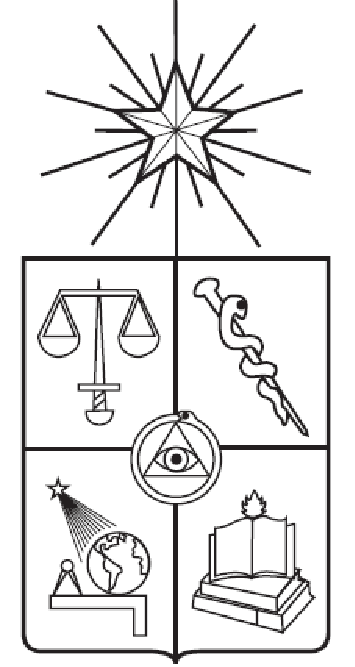
\includegraphics[width=1.5cm]{uchile3}
	\hspace{-0.2cm}
	\begin{tabular}{l}
		\COREwriteheaderitemsc[~\\]{\nombreuniversidad}
		\COREwriteheaderitemsc[~\\]{\nombrefacultad}
		\COREwriteheaderitemsc[~\\]{\departamentouniversidad}
		\vspace*{1cm}\mbox{}
	\end{tabular}
	\vfill
	\begin{center}
		\fontsize{8mm}{9mm}\selectfont
		\textcolor{\portraittitlecolor}{
			\noindent \titulodelinforme ~ \\
		}
		\vspace*{0.5cm}
		\Large{\noindent \textcolor{\portraittitlecolor}{\temaatratar}} ~ \\
		\vspace*{1cm}
		\footnotesize{\codigodelcurso\ - \nombredelcurso} ~ \\
		\vspace*{1.4cm}
	\end{center}
	\vfill
	\begin{center}
		\noindent \normalsize{\tablaintegrantes}
	\end{center}
}{
\ifthenelse{\equal{\portraitstyle}{style6}}{
	\setpagemargincm{\pagemarginleft}{\pagemargintop}{\pagemarginright}{\pagemarginbottom}
	\thispagestyle{empty}
	\begin{wrapfigure}{l}{0.3\textwidth}
		\vspace{-0.69cm}
		\noindent \hspace{-1.10cm} 
\includegraphics[scale=0.2]{img/LogoCS.png}
	\end{wrapfigure}
	\def\COREstylefirstmargin {-2.2cm}
	\ifthenelse{\equal{\departamentouniversidad}{\xspace}}{}{
		\hspace*{0.05cm}
		\noindent \textsc{\color{red} \hspace{\COREstylefirstmargin} \departamentouniversidad} ~ \\
		\def\COREstylefirstmargin {-1.6cm}
	}
	\ifthenelse{\equal{\nombrefacultad}{\xspace}}{}{
		\hspace*{0.05cm}
		\noindent \textsc{\color{dkgray} \hspace{\COREstylefirstmargin} \nombrefacultad} ~ \\
		\def\COREstylefirstmargin {-1.6cm}
	}
	\ifthenelse{\equal{\nombreuniversidad}{\xspace}}{}{
		\hspace*{0.05cm}
		\noindent \textsc{\color{dkgray} \hspace{\COREstylefirstmargin} \nombreuniversidad} ~ \\
		\def\COREstylefirstmargin {-1.6cm}
	}
	\ifthenelse{\equal{\nombredelcurso}{\xspace}}{}{
		\hspace*{0.05cm}
		\noindent \textsc{\color{dkgray} \hspace{\COREstylefirstmargin} \codigodelcurso \nombredelcurso} ~ \\
		\def\COREstylefirstmargin {-1.6cm}
	}
	\vfill
	\begin{center}
		\vspace*{0.5cm}
		{\color{dkgray} \Large \textbf{\MakeUppercase{\temaatratar}}} ~ \\
		\noindent \rule{\linewidth}{0.3mm} ~ \\
		\Huge \textup \bfseries \textsc{\textcolor{\portraittitlecolor}{\titulodelinforme}} ~ \\
		\noindent \rule{\linewidth}{0.3mm} ~ \\
	\end{center}
	\begin{minipage}{.5\textwidth}
		~
	\end{minipage}
	\vfill
	\begin{minipage}{1.0\textwidth}
		\begin{flushright}
			\noindent \tablaintegrantes
		\end{flushright}
	\end{minipage}
}{
\ifthenelse{\equal{\portraitstyle}{style7}}{
	\setpagemargincm{\pagemarginleft}{\pagemargintop}{\pagemarginright}{\pagemarginbottom}
	\thispagestyle{empty}
	\begin{center}
		\vspace*{-1.5cm}
		\includegraphics[scale=\imagendepartamentoescala]{\imagendepartamento}
		\hspace*{-0.15cm}
		\begin{tabular}{l}
			\vspace*{0.26cm}\mbox{} ~ \\
			\COREwriteheaderitemsc{\nombreuniversidad}
			\COREwriteheaderitemsc{\nombrefacultad}
			\COREwriteheaderitemsc{\departamentouniversidad}
			\vspace*{1.25cm}\mbox{}
		\end{tabular}
	\end{center}
	\vfill
	\begin{center}
		\noindent \rule{\textwidth}{0.4mm} \\ \vspace{0.3cm}
		{\huge \textcolor{\portraittitlecolor}{\titulodelinforme} \vspace{0.2cm} ~ \\}
		\noindent \rule{\textwidth}{0.4mm} ~ \\ \vspace{0.40cm}
		{\large \textcolor{\portraittitlecolor}{\temaatratar} ~ \\}
	\end{center}
	\vfill
	\noindent
	\begin{minipage}{1.0\textwidth}
		\begin{flushright}
			\scshape{\tablaintegrantes}
		\end{flushright}
	\end{minipage}
}{
\ifthenelse{\equal{\portraitstyle}{style8}}{
	\setpagemargincm{\pagemarginleft}{\pagemargintop}{\pagemarginright}{\pagemarginbottom}
	\thispagestyle{empty}
	\begin{center}
		\vspace*{-1.0cm}
		\begin{tabular}{c}
			\includegraphics[scale=\imagendepartamentoescala]{\imagendepartamento} \vspace{0.5cm} ~ \\
			\COREwriteheaderitemsc{\nombreuniversidad}
			\COREwriteheaderitemsc{\nombrefacultad}
			\COREwriteheaderitemsc{\departamentouniversidad}
		\end{tabular}
	\end{center}
	\vfill
	\begin{center}
		\noindent \rule{\textwidth}{0.4mm} \\ \vspace{0.3cm}
		{\huge \textcolor{\portraittitlecolor}{\titulodelinforme} \vspace{0.2cm} ~ \\}
		\noindent \rule{\textwidth}{0.4mm} ~ \\ \vspace{0.40cm}
		{\large \textcolor{\portraittitlecolor}{\temaatratar} ~ \\}
	\end{center}
	\vfill
	\noindent
	\begin{minipage}{1.0\textwidth}
		\begin{flushright}
			\scshape{\tablaintegrantes}
		\end{flushright}
	\end{minipage}
}{
\ifthenelse{\equal{\portraitstyle}{style9}}{
	\setpagemargincm{\pagemarginleft}{\pagemargintop}{\pagemarginright}{\pagemarginbottom}
	\thispagestyle{empty}
	\noindent \includegraphics[scale=\imagendepartamentoescala]{\imagendepartamento}
	\vfill
	\begin{center}
		\noindent \rule{\textwidth}{0.4mm} \\ \vspace{0.3cm}
		{\huge \textcolor{\portraittitlecolor}{\titulodelinforme} \vspace{0.2cm} \\}
		\noindent \rule{\textwidth}{0.4mm} \\ \vspace{0.35cm}
		{\large \textcolor{\portraittitlecolor}{\temaatratar} \\}
	\end{center}
	\vfill
	\begin{center}
		\begin{tabular}{c}
			\COREwriteheaderitemsc{\nombreuniversidad}
			\COREwriteheaderitemsc{\nombrefacultad}
			\COREwriteheaderitemsc{\departamentouniversidad}
		\end{tabular}
	\end{center}
	\vfill
	\begin{center}
		\indent \scshape{\tablaintegrantes}
	\end{center}
}{
\ifthenelse{\equal{\portraitstyle}{style10}}{
	\setpagemargincm{\pagemarginleft}{\pagemargintop}{\pagemarginright}{\pagemarginbottom}
	\thispagestyle{empty}
	~ \\
	\vfill
	\begin{center}
		\ifthenelse{\equal{\nombreuniversidad}{\xspace}}{
			\noindent {\large \textsc{\departamentouniversidad}}
		}{
			\noindent {\large \textsc{\nombreuniversidad, \departamentouniversidad}}
		}
		\vspace{1.0cm}
	\end{center}
	\vfill
	\begin{center}
		\ifthenelse{\equal{\nombredelcurso}{\xspace}}{}{
			\noindent {\large \scshape{\nombredelcurso}} \vspace{0.5cm} ~ \\
		}
		\ifthenelse{\equal{\codigodelcurso}{\xspace}}{}{
			\noindent {\large \scshape{\codigodelcurso}} \vspace{0.5cm} ~ \\
		}
		\noindent \rule{\textwidth}{0.4mm} \\ \vspace{0.3cm}
		{\huge \bfseries \textcolor{\portraittitlecolor}{\titulodelinforme} \vspace{0.2cm} \\}
		\noindent \rule{\textwidth}{0.4mm} \\ \vspace{2.5cm}
	\end{center}
	\vfill
	\begin{center}
		\indent \tablaintegrantes
	\end{center}
	\vfill
	~ \\
}{
\ifthenelse{\equal{\portraitstyle}{style11}}{
	\setpagemargincm{\pagemarginleft}{\pagemargintop}{\pagemarginright}{\pagemarginbottom}
	\thispagestyle{empty}
	\begin{center}
		\vspace*{-1.0cm}
		\ifthenelse{\equal{\nombreuniversidad}{\xspace}}{}{
			\scshape{\nombreuniversidad} ~ \\
		}
		\ifthenelse{\equal{\nombrefacultad}{\xspace}}{}{
			\scshape{\nombrefacultad} ~ \\
		}
		\ifthenelse{\equal{\departamentouniversidad}{\xspace}}{}{
			\scshape{\departamentouniversidad}
		}
	\end{center}
	\vfill
	\begin{center}
		{\setstretch{1.2} \fontsize{21pt}{22pt} \selectfont \textcolor{\portraittitlecolor}{\scshape{\titulodelinforme}} \vspace{0.5cm}} ~ \\
		{\fontsize{13pt}{10pt} \selectfont \textcolor{\portraittitlecolor}{\scshape{\temaatratar}}}
	\end{center}
	\vfill
	\begin{center}
		\indent \tablaintegrantes
	\end{center}
}{
\ifthenelse{\equal{\portraitstyle}{style12}}{
	\setpagemargincm{\pagemarginleft}{\pagemargintop}{\pagemarginright}{\pagemarginbottom}
	\thispagestyle{empty}
	\begin{center}
		\vspace*{-1.0cm}
		\includegraphics[scale=\imagendepartamentoescala]{\imagendepartamento}
	\end{center}
	\vfill
	\begin{center}
		{\bf \Huge \scshape{\textcolor{\portraittitlecolor}{\titulodelinforme}} \vspace{0.3cm}} \\
		{\bf \Large \textcolor{\portraittitlecolor}{\temaatratar}}
	\end{center}
	\vfill
	\begin{flushright}
		\noindent \tablaintegrantes
	\end{flushright}
	\vspace{0.5cm}
	\noindent \rule{\textwidth}{0.4mm}
	\begin{center}
		\ifthenelse{\equal{\nombreuniversidad}{\xspace}}{
			\scshape{\nombrefacultad} \\
		}{
			\scshape{\nombreuniversidad, \nombrefacultad} \\
		}
		\scshape{\departamentouniversidad}
	\end{center}
}{
\ifthenelse{\equal{\portraitstyle}{style13}}{
	\setpagemargincm{\pagemarginleft}{\pagemargintop}{\pagemarginright}{\pagemarginbottom}
	\thispagestyle{empty}
	\noindent
	\vspace*{-1.5cm}
	\begin{flushleft}
		\begin{minipage}{0.65\textwidth}
			\ifthenelse{\equal{\nombreuniversidad}{\xspace}}{
				{\fontsize{3.5mm}{0.5mm} \selectfont \noindent \textsf{\nombrefacultad}} ~ \\
			}{
				{\fontsize{3.5mm}{0.5mm} \selectfont \noindent \textsf{\nombreuniversidad, \nombrefacultad}} ~ \\
			}
			\noindent {\fontsize{3.0mm}{0.5mm} \selectfont \textsf{\departamentouniversidad} \vspace{-0.2cm}} ~ \\
			\noindent \textcolor{gray}{\rule{\textwidth}{0.3mm}}
		\end{minipage}
	\end{flushleft}
	\vspace*{-2.15cm}
	\begin{flushright}
		\begin{minipage}{0.3\textwidth}
			\noindent \includegraphics[width=1.0\textwidth]{\imagendepartamento}
		\end{minipage}
	\end{flushright}
	\vfill
	\begin{center}
		\begin{minipage}{0.9\textwidth}
			\begin{framed}
				\LARGE
				\vspace{1cm}
				\centering \textcolor{\portraittitlecolor}{\textbf{\titulodelinforme}}
				\vspace{1cm}
			\end{framed}
		\end{minipage}
	\end{center}
	\vfill
	\begin{flushright}
		\noindent \textsf{\tablaintegrantes}
	\end{flushright}
}{
\ifthenelse{\equal{\portraitstyle}{style14}}{
	\setpagemargincm{\pagemarginleft}{\pagemargintop}{\pagemarginright}{\pagemarginbottom}
	\thispagestyle{empty}
	\noindent
	\begin{flushleft}
		\vspace*{-1.0cm}
		\noindent \includegraphics[scale=\imagendepartamentoescala]{\imagendepartamento} \\
	\end{flushleft}
	\vfill
	{\bf \huge \noindent \textcolor{\portraittitlecolor}{\textsf{\MakeUppercase{\titulodelinforme}} \vspace*{0.05cm}}} \\
	{\bf \large \noindent \textcolor{\portraittitlecolor}{\textsf{\MakeUppercase{\temaatratar}}}} \\
	\vfill
	\begin{flushright}
		\noindent \textsf{\tablaintegrantes}
	\end{flushright}
}{
\ifthenelse{\equal{\portraitstyle}{style15}}{
	\setpagemargincm{\pagemarginleft}{\pagemargintop}{\pagemarginright}{\pagemarginbottom}
	\thispagestyle{empty}
	\checkextravarexist{\headerimageA}{Defina la imagen extra de la portada en el archivo lib/page/portrait-config.tex (VERSION NORMAL) o bien en el bloque PORTADA (VERSION COMPACTA)}
	\checkextravarexist{\headerimagescaleA}{Defina la escala de la imagen extra de la portada en el archivo lib/page/portrait-config.tex (VERSION NORMAL) o bien en el bloque PORTADA (VERSION COMPACTA)}
	\vspace*{-1.5cm}
	\noindent \begin{minipage}{0.8\textwidth}
		\noindent \begin{minipage}{0.22\textwidth}
			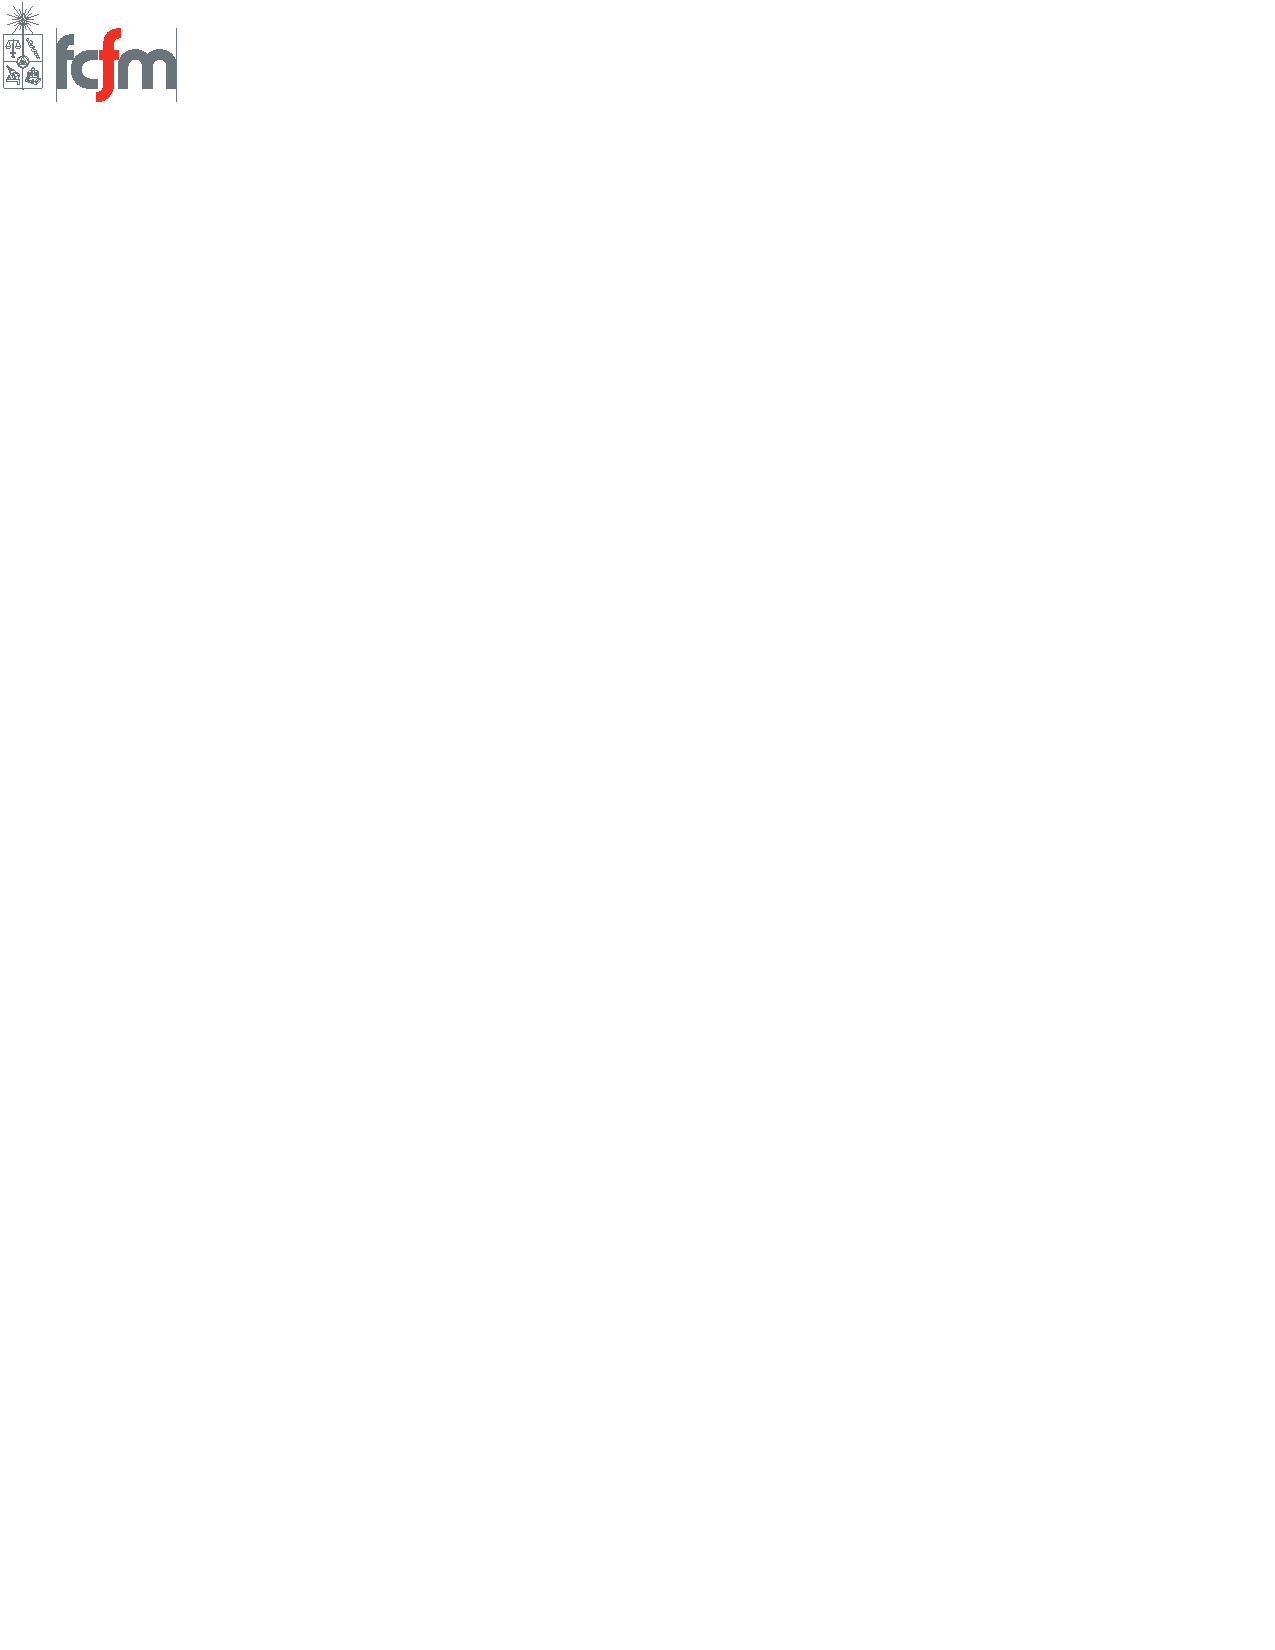
\includegraphics[scale=1.0]{fcfm2} \\
		\end{minipage}
		\begin{minipage}{0.6\textwidth}
			\begin{flushleft}
				\textsc{
				\begin{tabular}{l}
					\ifthenelse{\equal{\nombreuniversidad}{\xspace}}{}{
						{\small \nombreuniversidad} ~ \\
					}
					\ifthenelse{\equal{\nombrefacultad}{\xspace}}{}{
						{\small \nombrefacultad} ~ \\
					}
					\ifthenelse{\equal{\departamentouniversidad}{\xspace}}{}{
						{\small \departamentouniversidad}
					}
				\end{tabular}
				}
			\end{flushleft}
		\end{minipage}
	\end{minipage}
	\noindent \begin{minipage}{0.2\textwidth}
		\begin{flushright}
			\ifthenelse{\isundefined{\headerimageA}}{}{
				\ifthenelse{\isundefined{\headerimagescaleA}}{}{
					\noindent \includegraphics[scale=\headerimagescaleA]{\headerimageA} \\
				}
			}
		\end{flushright}
	\end{minipage}
	\vfill
	\begin{center}
		{\fontsize{25pt}{15pt} \selectfont \textcolor{\portraittitlecolor}{\textbf{\titulodelinforme}} \vspace{0.7cm}} \\
		{\Large \textcolor{\portraittitlecolor}{\temaatratar}}
	\end{center}
	\vfill
	\begin{center}
		\noindent \tablaintegrantes
	\end{center}
}{
\ifthenelse{\equal{\portraitstyle}{style16}}{
	\setpagemargincm{\pagemarginleft}{\pagemargintop}{\pagemarginright}{\pagemarginbottom}
	\checkextravarexist{\portraitbackgroundimageB}{[portrait-style16] Defina el fondo de la portada en el archivo lib/page/portrait-config.tex (VERSION NORMAL) o bien en el bloque PORTADA (VERSION COMPACTA)}
	\checkextravarexist{\portraitbackgroundcolorB}{[portrait-style16] Defina el color del bloque del titulo de la portada en el archivo lib/page/portrait-config.tex (VERSION NORMAL) o bien en el bloque PORTADA (VERSION COMPACTA)}
	\begingroup
		\thispagestyle{empty}
		\begin{tikzpicture}[remember picture,overlay]
			\node[inner sep=0pt] (background) at (current page.center) {\includegraphics[width=\paperwidth]{\portraitbackgroundimageB}};
			\draw (current page.center) node [fill=\portraitbackgroundcolorB!30!white,fill opacity=0.6,text opacity=1,inner sep=1cm]{\Huge\centering\bfseries\sffamily\parbox[c][][t]{\paperwidth}{
					\centering \textcolor{\portraittitlecolor}{\titulodelinforme} \\ [10pt]
					{\Large \textcolor{\portraittitlecolor}{\temaatratar}} \\ [25pt]
					{\huge \autordeldocumento}}};
		\end{tikzpicture}
		\vfill
	\endgroup
}{
\ifthenelse{\equal{\portraitstyle}{style17}}{
	\setpagemargincm{\pagemarginleft}{\firstpagemargintop}{\pagemarginright}{\pagemarginbottom}
	\pagestyle{fancy}
	\checkextravarexist{\portraitimageC}{[portrait-style17] Defina la imagen de la portada en el archivo lib/page/portrait-config.tex (VERSION NORMAL) o bien en el bloque PORTADA (VERSION COMPACTA)}
	\checkextravarexist{\portraitimageboxedC}{[portrait-style17] Defina si la imagen de la portada se encierra en un recuadro en el archivo lib/page/portrait-config.tex (VERSION NORMAL) o bien en el bloque PORTADA (VERSION COMPACTA)}
	\checkextravarexist{\portraitimageboxedwidthC}{[portrait-style17] Defina el grosor del recuadro de la imagen de la portada en el archivo lib/page/portrait-config.tex (VERSION NORMAL) o bien en el bloque PORTADA (VERSION COMPACTA)}
	\checkextravarexist{\portraitimagewidthC}{[portrait-style17] Defina los parametros de la imagen de la portada en el archivo lib/page/portrait-config.tex (VERSION NORMAL) o bien en el bloque PORTADA (VERSION COMPACTA)}
	\fancyhf{}
	\fancyhead[L]{
		\COREwriteheaderitem{\nombreuniversidad}
		\COREwriteheaderitem{\nombrefacultad}
		\COREwriteheaderitem{\departamentouniversidad}
		\vspace{-\baselineskip}
	}
	\fancyhead[R]{
		\includegraphics[scale=\imagendepartamentoescala]{\imagendepartamento}
		\hspace{-0.255cm}
		\vspace{-0.20cm}
	}
	~ \\
	\vfill
	\begin{center}
		\textcolor{\portraittitlecolor}{
			{\noindent \Huge{\titulodelinforme} \vspace{0.5cm}} ~ \\
			{\noindent \large{\temaatratar}}
		}
	\end{center}
	~ \\
	\ifthenelse{\equal{\portraitimageboxedC}{true}}{
		\insertimageboxed{\portraitimageC}{width=\portraitimagewidthC}{\portraitimageboxedwidthC}{}
	}{
		\insertimage{\portraitimageC}{width=\portraitimagewidthC}{}
	}
	~ \\
	\vfill
	\noindent
	\begin{minipage}{1.0\textwidth}
		\begin{flushright}
			\tablaintegrantes
		\end{flushright}
	\end{minipage}
}{
\ifthenelse{\equal{\portraitstyle}{style18}}{
	\setpagemargincm{\pagemarginleft}{\firstpagemargintop}{\pagemarginright}{\pagemarginbottom}
	\pagestyle{fancy}
	\checkextravarexist{\portraitimageD}{[portrait-style18] Defina la imagen de la portada en el archivo lib/page/portrait-config.tex (VERSION NORMAL) o bien en el bloque PORTADA (VERSION COMPACTA)}
	\checkextravarexist{\portraitimageboxedD}{[portrait-style18] Defina si la imagen de la portada se encierra en un recuadro en el archivo lib/page/portrait-config.tex (VERSION NORMAL) o bien en el bloque PORTADA (VERSION COMPACTA)}
	\checkextravarexist{\portraitimageboxedwidthD}{[portrait-style18] Defina el grosor del recuadro de la imagen de la portada en el archivo lib/page/portrait-config.tex (VERSION NORMAL) o bien en el bloque PORTADA (VERSION COMPACTA)}
	\checkextravarexist{\portraitimagewidthD}{[portrait-style18] Defina los parametros de la imagen de la portada en el archivo lib/page/portrait-config.tex (VERSION NORMAL) o bien en el bloque PORTADA (VERSION COMPACTA)}
	\fancyhf{}
	\fancyhead[L]{
		\COREwriteheaderitem{\nombreuniversidad}
		\COREwriteheaderitem{\nombrefacultad}
		\COREwriteheaderitem{\departamentouniversidad}
		\vspace{-\baselineskip}
	}
	\fancyhead[R]{
		\includegraphics[scale=\imagendepartamentoescala]{\imagendepartamento}
		\hspace{-0.255cm}
		\vspace{-0.20cm}
	}
	~ \\
	\ifthenelse{\equal{\portraitimageboxedD}{true}}{
		\insertimageboxed{\portraitimageD}{width=\portraitimagewidthD}{\portraitimageboxedwidthD}{}
	}{
		\insertimage{\portraitimageD}{width=\portraitimagewidthD}{}
	}
	\vfill
	\begin{center}
		\textcolor{\portraittitlecolor}{
			{\noindent \Huge{\titulodelinforme} \vspace{0.5cm}} ~ \\
			{\noindent \large{\temaatratar}}
		}
	\end{center}
	\vfill
	\noindent
	\begin{minipage}{1.0\textwidth}
		\begin{flushright}
			\tablaintegrantes
		\end{flushright}
	\end{minipage}
}{
\ifthenelse{\equal{\portraitstyle}{style19}}{
	\setpagemargincm{\pagemarginleft}{\pagemargintop}{\pagemarginright}{\pagemarginbottom}
	\thispagestyle{empty}
	\vspace*{0cm}
	\begin{center}
		\noindent \rule{\textwidth}{0.4mm} \\ \vspace{0.3cm}
		{\huge \bfseries \textcolor{\portraittitlecolor}{\titulodelinforme} \vspace{0.2cm} \\}
		\noindent \rule{\textwidth}{0.4mm}
	\end{center}
	~ \\
	\begin{center}
		\noindent {\large \scshape{\codigodelcurso} \large \scshape{\nombredelcurso}} \vspace{0.5cm} ~ \\
		\ifthenelse{\equal{\nombreuniversidad}{\xspace}}{
			\noindent {\large \textsc{\departamentouniversidad}}
		}{
			\noindent {\large \textsc{\nombreuniversidad, \departamentouniversidad}}
		}
		\vspace{1.0cm}
	\end{center}
	\vfill
	\begin{center}
		\indent \tablaintegrantes
	\end{center}
	~ \\
}{
\ifthenelse{\equal{\portraitstyle}{style20}}{
	\setpagemargincm{\pagemarginleft}{\pagemargintop}{\pagemarginright}{\pagemarginbottom}
	\thispagestyle{empty}
	{\raggedleft	
	\rule{1pt}{\textheight}
	\hspace{0.05\textwidth}
	\parbox[b]{0.75\textwidth}{
		{\Huge\bfseries \textcolor{\portraittitlecolor}{\titulodelinforme}}\\[2\baselineskip]
		{\large\textit{\textcolor{\portraittitlecolor}{\temaatratar}}}\\[4\baselineskip]
		\vspace*{2cm}
		{\textsc{
		\begin{flushleft}
			\noindent\tablaintegrantes
		\end{flushleft}
		}}
		\vspace*{\portraitverticalspaceE}
		{\noindent \nombreuniversidad ~\\
		\nombrefacultad ~\\
		\departamentouniversidad}\\[\baselineskip]
	}}
}{
\ifthenelse{\equal{\portraitstyle}{\bgtemplatetestcode}}{
	\setpagemargincm{\pagemarginleft}{\pagemargintop}{\pagemarginright}{\pagemarginbottom}
	\pagestyle{empty}
	\pagecolor{lbrown}
	\begin{center}
		\vspace*{-1.0cm}
		\ifthenelse{\equal{\nombreuniversidad}{\xspace}}{}{
			\scshape{\nombreuniversidad} ~ \\
		}
		\ifthenelse{\equal{\nombrefacultad}{\xspace}}{}{
			\scshape{\nombrefacultad} ~ \\
		}
		\ifthenelse{\equal{\departamentouniversidad}{\xspace}}{}{
			\scshape{\departamentouniversidad}
		}
	\end{center}
	~ \\
	\begin{center}
		\bgtemplatetestimg
	\end{center}
	\begin{center}
		\vspace*{-6cm}
		{\setstretch{1.2} \fontsize{25pt}{22pt} \selectfont \textcolor{\portraittitlecolor}{\scshape{\titulodelinforme}} \vspace{0.5cm}} \\
		{\fontsize{15pt}{10pt} \selectfont \textcolor{\portraittitlecolor}{\scshape{\temaatratar}}}
	\end{center}
	\vfill
	\begin{flushright}
		\noindent \tablaintegrantes
	\end{flushright}
	\newpage
	\pagecolor{\colorpage}
}{
	\throwbadconfigondoc{Estilo de portada incorrecto}{\portraitstyle}{style1 .. style20}}}}}}}}}}}}}}}}}}}}}
}
\ifthenelse{\equal{\addemptypagetwosides}{true}}{
	\newpage
	\null
	\thispagestyle{empty}
	\renewcommand{\thepage}{}
	\newpage}{
}
 % Se puede borrar

% CONFIGURACIÓN DE PÁGINA Y ENCABEZADOS
% Template:     Informe/Reporte LaTeX
% Documento:    Configuración de página
% Versión:      6.6.0 (19/09/2019)
% Codificación: UTF-8
%
% Autor: Pablo Pizarro R.
%        Facultad de Ciencias Físicas y Matemáticas
%        Universidad de Chile
%        pablo@ppizarror.com
%
% Manual template: [https://latex.ppizarror.com/informe]
% Licencia MIT:    [https://opensource.org/licenses/MIT]

\newpage
\ifthenelse{\equal{\predocpageromannumber}{true}}{
	\ifthenelse{\equal{\predocpageromanupper}{true}}{
		\pagenumbering{Roman}
	}{
		\pagenumbering{roman}
	}}{
	\pagenumbering{arabic}
}
\setcounter{page}{1}
\setcounter{footnote}{0}
\setpagemargincm{\pagemarginleft}{\pagemargintop}{\pagemarginright}{\pagemarginbottom}
\def\arraystretch {\tablepaddingv}
\setlength{\tabcolsep}{\tablepaddingh em}
\ifthenelse{\equal{\pointdecimal}{true}}{
	\decimalpoint}{
}
\renewcommand{\appendixname}{\nomltappendixsection}
\renewcommand{\appendixpagename}{\nameappendixsection}
\renewcommand{\appendixtocname}{\nameappendixsection}
\renewcommand{\contentsname}{\nomltcont}
\renewcommand{\figurename}{\nomltwfigure}
\renewcommand{\listfigurename}{\nomltfigure}
\renewcommand{\listtablename}{\nomlttable}
\renewcommand{\lstlistingname}{\nomltwsrc}
\renewcommand{\lstlistlistingname}{\nomltsrc}
\renewcommand{\refname}{\namereferences}
\renewcommand{\bibname}{\namereferences}
\renewcommand{\tablename}{\nomltwtable}
\sectionfont{\color{\titlecolor} \fontsizetitle \styletitle \selectfont}
\subsectionfont{\color{\subtitlecolor} \fontsizesubtitle \stylesubtitle \selectfont}
\subsubsectionfont{\color{\subsubtitlecolor} \fontsizesubsubtitle \stylesubsubtitle \selectfont}
\titleformat{\subsubsubsection}{\color{\ssstitlecolor} \normalfont \fontsizessstitle \stylessstitle}{\thesubsubsubsection}{1em}{}
\titlespacing*{\subsubsubsection}{0pt}{3.25ex plus 1ex minus .2ex}{1.5ex plus .2ex}
\fancyheadoffset{0pt}
\def\hfheaderimagesizeA {1.2}
\ifthenelse{\equal{\hfstyle}{style1}}{
	\pagestyle{fancy}
	\newcommand{\COREstyledefinition}{
		\fancyhf{}
		\ifthenelse{\equal{\disablehfrightmark}{false}}{
			\fancyhead[L]{\nouppercase{\rightmark}}
		}{}
		\fancyhead[R]{\small \thepage}
		\ifthenelse{\equal{\hfwidthwrap}{true}}{
			\fancyfoot[L]{
				\begin{minipage}[t]{\hfwidthtitle\linewidth}
					\begin{flushleft}
						\small \textit{\titulodelinforme}
					\end{flushleft}
				\end{minipage}
			}
			\fancyfoot[R]{
				\begin{minipage}[t]{\hfwidthcourse\linewidth}
					\begin{flushright}
						\small \textit{\codigodelcurso \nombredelcurso}
					\end{flushright}
				\end{minipage}
			}
		}{
			\fancyfoot[L]{\small \textit{\titulodelinforme}}
			\fancyfoot[R]{\small \textit{\codigodelcurso \nombredelcurso}}
		}
		\renewcommand{\headrulewidth}{0.5pt}
		\renewcommand{\footrulewidth}{0.5pt}
	}
	\renewcommand{\sectionmark}[1]{\markboth{#1}{}}
	\COREstyledefinition
}{
\ifthenelse{\equal{\hfstyle}{style2}}{
	\pagestyle{fancy}
	\newcommand{\COREstyledefinition}{
		\fancyhf{}
		\ifthenelse{\equal{\disablehfrightmark}{false}}{
			\fancyhead[L]{\nouppercase{\rightmark}}
		}{}
		\fancyhead[R]{\small \thepage}
		\ifthenelse{\equal{\hfwidthwrap}{true}}{
			\fancyfoot[L]{
				\begin{minipage}[t]{\hfwidthtitle\linewidth}
					\begin{flushleft}
						\small \textit{\titulodelinforme}
					\end{flushleft}
				\end{minipage}
			}
			\fancyfoot[R]{
				\begin{minipage}[t]{\hfwidthcourse\linewidth}
					\begin{flushright}
						\small \textit{\codigodelcurso \nombredelcurso}
					\end{flushright}
				\end{minipage}
			}
		}{
			\fancyfoot[L]{\small \textit{\titulodelinforme}}
			\fancyfoot[R]{\small \textit{\codigodelcurso \nombredelcurso}}
		}
		\renewcommand{\headrulewidth}{0.5pt}
		\renewcommand{\footrulewidth}{0pt}
	}
	\renewcommand{\sectionmark}[1]{\markboth{#1}{}}
	\COREstyledefinition
}{
\ifthenelse{\equal{\hfstyle}{style3}}{
	\pagestyle{fancy}
	\newcommand{\COREstyledefinition}{
		\fancyhf{}
		\ifthenelse{\equal{\hfwidthwrap}{true}}{
			\fancyhead[L]{
				\begin{minipage}[t]{\hfwidthtitle\linewidth}
					\begin{flushleft}
						\small \textit{\codigodelcurso \nombredelcurso}
					\end{flushleft}
				\end{minipage}
			}
		}{
			\fancyhead[L]{\small \textit{\codigodelcurso \nombredelcurso}}
		}
		\fancyhead[R]{
			\includegraphics[width=\hfheaderimagesizeA cm]{\imagendepartamento}
			\vspace{-0.15cm}
		}
		\fancyfoot[C]{\thepage}
		\renewcommand{\headrulewidth}{0.5pt}
		\renewcommand{\footrulewidth}{0pt}
	}
	\COREstyledefinition
}{
\ifthenelse{\equal{\hfstyle}{style4}}{
	\pagestyle{fancy}
	\newcommand{\COREstyledefinition}{
		\fancyhf{}
		\ifthenelse{\equal{\disablehfrightmark}{false}}{
			\fancyhead[L]{\nouppercase{\rightmark}}
		}{}
		\fancyhead[R]{}
		\fancyfoot[C]{\small \thepage}
		\renewcommand{\headrulewidth}{0.5pt}
		\renewcommand{\footrulewidth}{0pt}
	}
	\renewcommand{\sectionmark}[1]{\markboth{#1}{}}
	\COREstyledefinition
}{
\ifthenelse{\equal{\hfstyle}{style5}}{
	\pagestyle{fancy}
	\newcommand{\COREstyledefinition}{
		\fancyhf{}
		\ifthenelse{\equal{\hfwidthwrap}{true}}{
			\fancyhead[L]{
				\begin{minipage}[t]{\hfwidthcourse\linewidth}
					\begin{flushleft}
						\codigodelcurso \nombredelcurso
					\end{flushleft}
				\end{minipage}
			}
			\ifthenelse{\equal{\disablehfrightmark}{false}}{
				\fancyhead[R]{
					\begin{minipage}[t]{\hfwidthtitle\linewidth}
						\begin{flushright}
							\nouppercase{\rightmark}
						\end{flushright}
					\end{minipage}
				}
			}{}
		}{
			\fancyhead[L]{\codigodelcurso \nombredelcurso}
			\ifthenelse{\equal{\disablehfrightmark}{false}}{
				\fancyhead[R]{\nouppercase{\rightmark}}
			}{}
		}
		\fancyfoot[L]{\departamentouniversidad, \nombreuniversidad}
		\fancyfoot[R]{\small \thepage}
		\renewcommand{\headrulewidth}{0pt}
		\renewcommand{\footrulewidth}{0pt}
	}
	\renewcommand{\sectionmark}[1]{\markboth{#1}{}}
	\COREstyledefinition
}{
\ifthenelse{\equal{\hfstyle}{style6}}{
	\pagestyle{fancy}
	\newcommand{\COREstyledefinition}{
		\fancyhf{}
		\fancyfoot[L]{\departamentouniversidad}
		\fancyfoot[C]{\thepage}
		\fancyfoot[R]{\nombreuniversidad}
		\renewcommand{\headrulewidth}{0pt}
		\renewcommand{\footrulewidth}{0pt}
	}
	\setlength{\headheight}{49pt}
	\COREstyledefinition
}{
\ifthenelse{\equal{\hfstyle}{style7}}{
	\pagestyle{fancy}
	\newcommand{\COREstyledefinition}{
		\fancyhf{}
		\fancyfoot[C]{\thepage}
		\renewcommand{\headrulewidth}{0pt}
		\renewcommand{\footrulewidth}{0pt}
	}
	\setlength{\headheight}{49pt}
	\COREstyledefinition
}{
\ifthenelse{\equal{\hfstyle}{style8}}{
	\pagestyle{fancy}
	\newcommand{\COREstyledefinition}{
		\fancyhf{}
		\fancyfoot[R]{\thepage}
		\renewcommand{\headrulewidth}{0pt}
		\renewcommand{\footrulewidth}{0pt}
	}
	\setlength{\headheight}{49pt}
	\COREstyledefinition
}{
\ifthenelse{\equal{\hfstyle}{style9}}{
	\pagestyle{fancy}
	\newcommand{\COREstyledefinition}{
		\fancyhf{}
		\ifthenelse{\equal{\disablehfrightmark}{false}}{
			\fancyhead[L]{\nouppercase{\rightmark}}
		}{}
		\fancyhead[R]{}
		\fancyfoot[L]{\small \textit{\titulodelinforme}}
		\fancyfoot[R]{\small \thepage}
		\renewcommand{\headrulewidth}{0.5pt}
		\renewcommand{\footrulewidth}{0.5pt}
	}
	\renewcommand{\sectionmark}[1]{\markboth{#1}{}}
	\COREstyledefinition
}{
\ifthenelse{\equal{\hfstyle}{style10}}{
	\pagestyle{fancy}
	\newcommand{\COREstyledefinition}{
		\fancyhf{}
		\ifthenelse{\equal{\hfwidthwrap}{true}}{
			\ifthenelse{\equal{\disablehfrightmark}{false}}{
				\fancyhead[L]{
					\begin{minipage}[t]{\hfwidthtitle\linewidth}
						\begin{flushleft}
							\nouppercase{\rightmark}
						\end{flushleft}
					\end{minipage}
				}
			}{}
			\fancyhead[R]{
				\begin{minipage}[t]{\hfwidthcourse\linewidth}
					\begin{flushright}
						\small \textit{\titulodelinforme}
					\end{flushright}
				\end{minipage}
			}
		}{
			\ifthenelse{\equal{\disablehfrightmark}{false}}{
				\fancyhead[L]{\nouppercase{\rightmark}}
			}{}
			\fancyhead[R]{\small \textit{\titulodelinforme}}
		}
		\fancyfoot[L]{}
		\fancyfoot[R]{\small \thepage}
		\renewcommand{\headrulewidth}{0.5pt}
		\renewcommand{\footrulewidth}{0.5pt}
	}
	\renewcommand{\sectionmark}[1]{\markboth{#1}{}}
	\COREstyledefinition
}{
\ifthenelse{\equal{\hfstyle}{style11}}{
	\pagestyle{fancy}
	\newcommand{\COREstyledefinition}{
		\fancyhf{}
		\ifthenelse{\equal{\disablehfrightmark}{false}}{
			\fancyhead[L]{\nouppercase{\rightmark}}
		}{}
		\fancyhead[R]{\small \thepage \nomnpageof \pageref{LastPage}}
		\ifthenelse{\equal{\hfwidthwrap}{true}}{
			\fancyfoot[L]{
				\begin{minipage}[t]{\hfwidthtitle\linewidth}
					\begin{flushleft}
						\small \textit{\titulodelinforme}
					\end{flushleft}
				\end{minipage}
			}
			\fancyfoot[R]{
				\begin{minipage}[t]{\hfwidthcourse\linewidth}
					\begin{flushright}
						\small \textit{\codigodelcurso \nombredelcurso}
					\end{flushright}
				\end{minipage}
			}
		}{
			\fancyfoot[L]{\small \textit{\titulodelinforme}}
			\fancyfoot[R]{\small \textit{\codigodelcurso \nombredelcurso}}
		}
		\renewcommand{\headrulewidth}{0.5pt}
		\renewcommand{\footrulewidth}{0.5pt}
	}
	\renewcommand{\sectionmark}[1]{\markboth{#1}{}}
	\COREstyledefinition
}{
\ifthenelse{\equal{\hfstyle}{style12}}{
	\pagestyle{fancy}
	\newcommand{\COREstyledefinition}{
		\fancyhf{}
		\fancyfoot[L]{\departamentouniversidad}
		\fancyfoot[C]{\thepage \nomnpageof \pageref{LastPage}}
		\fancyfoot[R]{\nombreuniversidad}
		\renewcommand{\headrulewidth}{0pt}
		\renewcommand{\footrulewidth}{0pt}
	}
	\setlength{\headheight}{49pt}
	\COREstyledefinition
}{
\ifthenelse{\equal{\hfstyle}{style13}}{
	\pagestyle{fancy}
	\newcommand{\COREstyledefinition}{
		\fancyhf{}
		\ifthenelse{\equal{\hfwidthwrap}{true}}{
			\fancyhead[L]{
				\begin{minipage}[t]{\hfwidthtitle\linewidth}
					\begin{flushleft}
						\small \textit{\codigodelcurso \nombredelcurso}
					\end{flushleft}
				\end{minipage}
			}
		}{
			\fancyhead[L]{\small \textit{\codigodelcurso \nombredelcurso}}
		}
		\fancyhead[R]{
			\includegraphics[width=\hfheaderimagesizeA cm]{\imagendepartamento}
			\vspace{-0.15cm}
		}
		\fancyfoot[C]{\thepage \nomnpageof \pageref{LastPage}}
		\renewcommand{\headrulewidth}{0.5pt}
		\renewcommand{\footrulewidth}{0pt}
	}
	\COREstyledefinition
}{
\ifthenelse{\equal{\hfstyle}{style14}}{
	\pagestyle{fancy}
	\newcommand{\COREstyledefinition}{
		\fancyhf{}
		\ifthenelse{\equal{\disablehfrightmark}{false}}{
			\fancyhead[L]{\nouppercase{\rightmark}}
		}{}
		\fancyhead[R]{}
		\fancyfoot[C]{\small \thepage \nomnpageof \pageref{LastPage}}
		\renewcommand{\headrulewidth}{0.5pt}
		\renewcommand{\footrulewidth}{0pt}
	}
	\renewcommand{\sectionmark}[1]{\markboth{#1}{}}
	\COREstyledefinition
}{
\ifthenelse{\equal{\hfstyle}{style15}}{
	\pagestyle{fancy}
	\newcommand{\COREstyledefinition}{
		\fancyhf{}
		\ifthenelse{\equal{\disablehfrightmark}{false}}{
			\fancyhead[L]{\nouppercase{\rightmark}}
		}{}
		\fancyhead[R]{}
		\fancyfoot[L]{
			\small \codigodelcurso \nombredelcurso
		}
		\fancyfoot[R]{
			\small \thepage
		}
		\renewcommand{\headrulewidth}{0.5pt}
		\renewcommand{\footrulewidth}{0.5pt}
	}
	\renewcommand{\sectionmark}[1]{\markboth{#1}{}}
	\COREstyledefinition
}{
\ifthenelse{\equal{\hfstyle}{style16}}{
	\pagestyle{fancy}
	\newcommand{\COREstyledefinition}{
		\fancyhf{}
		\renewcommand{\headrulewidth}{0pt}
		\renewcommand{\footrulewidth}{0pt}
	}
	\renewcommand{\sectionmark}[1]{\markboth{#1}{}}
	\COREstyledefinition
}{
	\throwbadconfigondoc{Estilo de header-footer incorrecto}{\hfstyle}{style1 .. style16}}}}}}}}}}}}}}}}
}
\fancypagestyle{plain}{
	\fancyheadoffset{0pt}
	\COREstyledefinition
}
\ifthenelse{\equal{\showlinenumbers}{true}}{
	\linenumbers}{
}


El presente apunte contiene los contenidos del curso MA4402 Simulación Estocástica: Teoría y Laboratorio. Este curso es de carácter obligatorio para la carrera de Ingeniería Civil Matemática de la Universidad de Chile.

\newp La versión presentada en este texto fue mayormente desarrollada entre los meses de agosto 2021 y agosto 2022, y toma como base, para las cinco primeras unidades, el curso tal como fue dictado el semestre de primavera 2021. Para la unidad \ref{browniano}, se utilizaron anotaciones del curso dictado en años anteriores por Roberto Cortez. La transcripción y edición de todo el texto fue realizada por Camilo Carvajal. 

\newpage
% TABLA DE CONTENIDOS - ÍNDICE
% Template:     Informe/Reporte LaTeX
% Documento:    Índice
% Versión:      6.6.0 (19/09/2019)
% Codificación: UTF-8
%
% Autor: Pablo Pizarro R.
%        Facultad de Ciencias Físicas y Matemáticas
%        Universidad de Chile
%        pablo@ppizarror.com
%
% Manual template: [https://latex.ppizarror.com/informe]
% Licencia MIT:    [https://opensource.org/licenses/MIT]

\ifthenelse{\equal{\showindex}{true}}{
	\newpage
	\begingroup
	\sectionfont{\color{\indextitlecolor} \fontsizetitlei \styletitlei \selectfont}
	\ifthenelse{\equal{\addemptypagetwosides}{true}}{
		\checkoddpage
		\ifoddpage
		\else
			\newpage
			\null
			\thispagestyle{empty}
			\newpage
			\addtocounter{page}{-1}
		\fi}{
	}
	\ifthenelse{\equal{\addindextobookmarks}{true}}{
		\belowpdfbookmark{\nomltcont}{contents}}{
	}
	\tocloftpagestyle{fancy}
	\ifthenelse{\equal{\showdotaftersnum}{true}}{		
		\def\cftchapaftersnum {.}
		\def\cftsecaftersnum {.}
		\def\cftsubsecaftersnum {.}
		\def\cftsubsubsecaftersnum {.}
		\def\cftsubsubsubsecaftersnum {.}
		\def\cftsecnumwidth {1.9em}
\def\cftsubsecnumwidth {2.57em}
\renewcommand\cftsubsubsecnumwidth{3.35em}
		\setlength{\cftsubsecindent}{1.91em}
\setlength{\cftsubsubsecindent}{4.48em}
		}{
	}
	\renewcommand{\cftdot}{\charnumpageindex}
	\def\cftfigaftersnum {\charafterobjectindex\enspace}
	\def\cftsubfigaftersnum {\charafterobjectindex\enspace}
	\def\cfttabaftersnum {\charafterobjectindex\enspace}
	\def\cftlstlistingaftersnum {\charafterobjectindex\enspace}
	\ifthenelse{\equal{\showlinenumbers}{true}}{
		\nolinenumbers}{
	}
	\ifthenelse{\equal{\objectindexindent}{true}}{
		\setlength{\cfttabindent}{1.9em}
		\setlength{\cftfigindent}{1.9em}
		\setlength{\cftsubfigindent}{1.9em}
		\def\cftlstlistingindent {1.9em}
	}{
		\setlength{\cfttabindent}{0em}
		\setlength{\cftfigindent}{0em}
		\setlength{\cftsubfigindent}{0em}
		\def\cftlstlistingindent {0em}
	}
	\ifthenelse{\equal{\showsectioncaptioncode}{none}}{
\def\cftdefautnumwidthcode {3.0em}
\def\cftdefaultnumwidthromancode {5.25em}
	}{
	\ifthenelse{\equal{\showsectioncaptioncode}{sec}}{
		\def\cftdefautnumwidthcode {3.7em}
		\def\cftdefaultnumwidthromancode {5.75em}
	}{
	\ifthenelse{\equal{\showsectioncaptioncode}{ssec}}{
		\def\cftdefautnumwidthcode {4.4em}
		\def\cftdefaultnumwidthromancode {6.25em}
	}{
	\ifthenelse{\equal{\showsectioncaptioncode}{sssec}}{
		\def\cftdefautnumwidthcode {5.1em}
		\def\cftdefaultnumwidthromancode {6.75em}
	}{
	\ifthenelse{\equal{\showsectioncaptioncode}{ssssec}}{
		\def\cftdefautnumwidthcode {5.8em}
		\def\cftdefaultnumwidthromancode {7.25em}
	}{
	\ifthenelse{\equal{\showsectioncaptioncode}{chap}}{
		\def\cftdefautnumwidthcode {3.0em}
		\def\cftdefaultnumwidthromancode {5.25em}
	}{
		\throwbadconfig{Valor configuracion incorrecto}{\showsectioncaptioncode}{none,chap,sec,ssec,sssec,ssssec}}}}}}
	}
	\ifthenelse{\equal{\showsectioncaptionfig}{none}}{
\def\cftdefautnumwidthfig {3.0em}
\def\cftdefaultnumwidthromanfig {5.25em}
	}{
	\ifthenelse{\equal{\showsectioncaptionfig}{sec}}{
		\def\cftdefautnumwidthfig {3.7em}
		\def\cftdefaultnumwidthromanfig {5.75em}
	}{
	\ifthenelse{\equal{\showsectioncaptionfig}{ssec}}{
		\def\cftdefautnumwidthfig {4.4em}
		\def\cftdefaultnumwidthromanfig {6.25em}
	}{
	\ifthenelse{\equal{\showsectioncaptionfig}{sssec}}{
		\def\cftdefautnumwidthfig {5.1em}
		\def\cftdefaultnumwidthromanfig {6.75em}
	}{
	\ifthenelse{\equal{\showsectioncaptionfig}{ssssec}}{
		\def\cftdefautnumwidthfig {5.8em}
		\def\cftdefaultnumwidthromanfig {7.25em}
	}{
	\ifthenelse{\equal{\showsectioncaptionfig}{chap}}{
		\def\cftdefautnumwidthfig {3.0em}
		\def\cftdefaultnumwidthromanfig {5.25em}
	}{
		\throwbadconfig{Valor configuracion incorrecto}{\showsectioncaptionfig}{none,chap,sec,ssec,sssec,ssssec}}}}}}
	}
	\ifthenelse{\equal{\showsectioncaptiontab}{none}}{
\def\cftdefautnumwidthtab {3.0em}
\def\cftdefaultnumwidthromantab {5.25em}
	}{
	\ifthenelse{\equal{\showsectioncaptiontab}{sec}}{
		\def\cftdefautnumwidthtab {3.7em}
		\def\cftdefaultnumwidthromantab {5.75em}
	}{
	\ifthenelse{\equal{\showsectioncaptiontab}{ssec}}{
		\def\cftdefautnumwidthtab {4.4em}
		\def\cftdefaultnumwidthromantab {6.25em}
	}{
	\ifthenelse{\equal{\showsectioncaptiontab}{sssec}}{
		\def\cftdefautnumwidthtab {5.1em}
		\def\cftdefaultnumwidthromantab {6.75em}
	}{
	\ifthenelse{\equal{\showsectioncaptiontab}{ssssec}}{
		\def\cftdefautnumwidthtab {5.8em}
		\def\cftdefaultnumwidthromantab {7.25em}
	}{
	\ifthenelse{\equal{\showsectioncaptiontab}{chap}}{
		\def\cftdefautnumwidthtab {3.0em}
		\def\cftdefaultnumwidthromantab {5.25em}
	}{
		\throwbadconfig{Valor configuracion incorrecto}{\showsectioncaptiontab}{none,chap,sec,ssec,sssec,ssssec}}}}}}
	}
	\def\cftfignumwidth {\cftdefautnumwidth}
	\def\cfttabnumwidth {\cftdefautnumwidth}
	\def\cftlstlistingnumwidth {\cftdefautnumwidth}
\ifthenelse{\equal{\captionnumcode}{arabic}}{
		\def\cftlstlistingnumwidth {\cftdefautnumwidthcode}
	}{
		\ifthenelse{\equal{\captionnumcode}{roman}}{
			\def\cftlstlistingnumwidth {\cftdefaultnumwidthromancode}
		}{
		\ifthenelse{\equal{\captionnumcode}{Roman}}{
			\def\cftlstlistingnumwidth {\cftdefaultnumwidthromancode}
		}{
			\def\cftlstlistingnumwidth {\cftdefautnumwidthcode}
		}}
	}
\ifthenelse{\equal{\captionnumfigure}{arabic}}{
		\def\cftfignumwidth {\cftdefautnumwidthfig}
	}{
		\ifthenelse{\equal{\captionnumfigure}{roman}}{
			\def\cftfignumwidth {\cftdefaultnumwidthromanfig}
		}{
			\ifthenelse{\equal{\captionnumfigure}{Roman}}{
				\def\cftfignumwidth {\cftdefaultnumwidthromanfig}
			}{
				\def\cftfignumwidth {\cftdefautnumwidthfig}
			}}
	}
\ifthenelse{\equal{\captionnumtable}{arabic}}{
		\def\cfttabnumwidth {\cftdefautnumwidthtab}
	}{
		\ifthenelse{\equal{\captionnumtable}{roman}}{
			\def\cfttabnumwidth {\cftdefaultnumwidthromantab}
		}{
			\ifthenelse{\equal{\captionnumtable}{Roman}}{
				\def\cfttabnumwidth {\cftdefaultnumwidthromantab}
			}{
				\def\cfttabnumwidth {\cftdefautnumwidthtab}
			}}
	}
	\newcommand{\coregeneratefigureindex}{
		\iftotalfigures
			\ifthenelse{\equal{\indexnewpagef}{true}}{\newpage}{}
			\listoffigures
		\fi
	}
	\newcommand{\coregeneratetableindex}{
		\iftotaltables
			\ifthenelse{\equal{\indexnewpaget}{true}}{\newpage}{}
			\listoftables
		\fi
	}
	\newcommand{\coregeneratecodeindex}{
		\iftotallstlistings
			\ifthenelse{\equal{\indexnewpagec}{true}}{\newpage}{}
			\lstlistoflistings
		\fi
	}
	\ifthenelse{\equal{\showindexofcontents}{true}}{
		\tableofcontents
	}{}
	\ifthenelse{\equal{\indexstyle}{ftc}}{
		\coregeneratefigureindex
		\coregeneratetableindex
		\coregeneratecodeindex
	}{
	\ifthenelse{\equal{\indexstyle}{f}}{
		\coregeneratefigureindex
	}{
	\ifthenelse{\equal{\indexstyle}{ft}}{
		\coregeneratefigureindex
		\coregeneratetableindex
	}{
	\ifthenelse{\equal{\indexstyle}{fc}}{
		\coregeneratefigureindex
		\coregeneratecodeindex
	}{
	\ifthenelse{\equal{\indexstyle}{fct}}{
		\coregeneratefigureindex
		\coregeneratecodeindex
		\coregeneratetableindex
	}{
	\ifthenelse{\equal{\indexstyle}{t}}{
		\coregeneratetableindex
	}{
	\ifthenelse{\equal{\indexstyle}{tf}}{
		\coregeneratetableindex
		\coregeneratefigureindex
	}{
	\ifthenelse{\equal{\indexstyle}{tfc}}{
		\coregeneratetableindex
		\coregeneratefigureindex
		\coregeneratecodeindex
	}{
	\ifthenelse{\equal{\indexstyle}{tc}}{
		\coregeneratetableindex
		\coregeneratecodeindex
	}{
	\ifthenelse{\equal{\indexstyle}{tcf}}{
		\coregeneratetableindex
		\coregeneratecodeindex
		\coregeneratefigureindex
	}{
	\ifthenelse{\equal{\indexstyle}{c}}{
		\coregeneratecodeindex
	}{
	\ifthenelse{\equal{\indexstyle}{ct}}{
		\coregeneratecodeindex
		\coregeneratetableindex
	}{
	\ifthenelse{\equal{\indexstyle}{ctf}}{
		\coregeneratecodeindex
		\coregeneratetableindex
		\coregeneratefigureindex
	}{
	\ifthenelse{\equal{\indexstyle}{cf}}{
		\coregeneratecodeindex
		\coregeneratefigureindex
	}{
	\ifthenelse{\equal{\indexstyle}{cft}}{
		\coregeneratecodeindex
		\coregeneratefigureindex
		\coregeneratetableindex
	}{
	\ifthenelse{\equal{\indexstyle}{}}{
	}{
		\throwbadconfig{Estilo desconocido del indice}{\indexstyle}{,f,ft,ftc,fc,fct,t,tf,tfc,tc,tcf,c,ct,ctf,cf,cft}}}}}}}}}}}}}}}}
	}
	\endgroup
	\newpage
	\ifthenelse{\equal{\addemptypagetwosides}{true}}{
		\vfill
		\checkoddpage
		\ifoddpage
			\newpage
			\null
			\thispagestyle{empty}
			\newpage
			\addtocounter{page}{-1}
		\else
		\fi}{
	}
}{}
 % Se puede borrar

% CONFIGURACIONES FINALES
% Template:     Informe/Reporte LaTeX
% Documento:    Configuraciones finales
% Versión:      6.6.0 (19/09/2019)
% Codificación: UTF-8
%
% Autor: Pablo Pizarro R.
%        Facultad de Ciencias Físicas y Matemáticas
%        Universidad de Chile
%        pablo@ppizarror.com
%
% Manual template: [https://latex.ppizarror.com/informe]
% Licencia MIT:    [https://opensource.org/licenses/MIT]

\markboth{}{}
\newpage
\ifthenelse{\equal{\disablehfrightmark}{false}}{
	\ifthenelse{\equal{\hfstyle}{style1}}{
		\fancypagestyle{plain}{\fancyhead[L]{\nouppercase{\leftmark}}}
		\fancyhead[L]{\nouppercase{\leftmark}}}{
	}
	\ifthenelse{\equal{\hfstyle}{style2}}{
		\fancypagestyle{plain}{\fancyhead[L]{\nouppercase{\leftmark}}}
		\fancyhead[L]{\nouppercase{\leftmark}}}{
	}
	\ifthenelse{\equal{\hfstyle}{style4}}{
		\fancypagestyle{plain}{\fancyhead[L]{\nouppercase{\leftmark}}}
		\fancyhead[L]{\nouppercase{\leftmark}}}{
	}
	\ifthenelse{\equal{\hfstyle}{style5}}{
		\fancypagestyle{plain}{
			\ifthenelse{\equal{\hfwidthwrap}{true}}{
				\fancyhead[R]{
					\begin{minipage}[t]{\hfwidthtitle\linewidth}
						\begin{flushright}
							\nouppercase{\leftmark}
						\end{flushright}
					\end{minipage}
				}
			}{
				\fancyhead[R]{\nouppercase{\leftmark}}
			}
		}
		\ifthenelse{\equal{\hfwidthwrap}{true}}{
			\fancyhead[R]{
				\begin{minipage}[t]{\hfwidthtitle\linewidth}
					\begin{flushright}
						\nouppercase{\leftmark}
					\end{flushright}
				\end{minipage}
			}
		}{
			\fancyhead[R]{\nouppercase{\leftmark}}
		}}{
	}
	\ifthenelse{\equal{\hfstyle}{style9}}{
		\fancypagestyle{plain}{\fancyhead[L]{\nouppercase{\leftmark}}}
		\fancyhead[L]{\nouppercase{\leftmark}}}{
	}
	\ifthenelse{\equal{\hfstyle}{style10}}{
		\fancypagestyle{plain}{
			\ifthenelse{\equal{\hfwidthwrap}{true}}{
				\fancyhead[L]{
					\begin{minipage}[t]{\hfwidthtitle\linewidth}
						\begin{flushleft}
							\nouppercase{\leftmark}
						\end{flushleft}
					\end{minipage}
				}
			}{
				\fancyhead[L]{\nouppercase{\leftmark}}
			}
		}
		\ifthenelse{\equal{\hfwidthwrap}{true}}{
			\fancyhead[L]{
				\begin{minipage}[t]{\hfwidthtitle\linewidth}
					\begin{flushleft}
						\nouppercase{\leftmark}
					\end{flushleft}
				\end{minipage}
			}
		}{
			\fancyhead[L]{\nouppercase{\leftmark}}
		}}{
	}
\ifthenelse{\equal{\hfstyle}{style11}}{
		\fancypagestyle{plain}{\fancyhead[L]{\nouppercase{\leftmark}}}
		\fancyhead[L]{\nouppercase{\leftmark}}}{
	}
\ifthenelse{\equal{\hfstyle}{style14}}{
		\fancypagestyle{plain}{\fancyhead[L]{\nouppercase{\leftmark}}}
		\fancyhead[L]{\nouppercase{\leftmark}}}{
	}
\ifthenelse{\equal{\hfstyle}{style15}}{
		\fancypagestyle{plain}{\fancyhead[L]{\nouppercase{\leftmark}}}
		\fancyhead[L]{\nouppercase{\leftmark}}}{
	}
	}{
}
\sectionfont{\color{\titlecolor} \fontsizetitle \styletitle \selectfont}
\subsectionfont{\color{\subtitlecolor} \fontsizesubtitle \stylesubtitle \selectfont}
\subsubsectionfont{\color{\subsubtitlecolor} \fontsizesubsubtitle \stylesubsubtitle \selectfont}
\titleformat{\subsubsubsection}{\color{\ssstitlecolor} \normalfont \fontsizessstitle \stylessstitle}{\thesubsubsubsection}{1em}{}
\titlespacing*{\subsubsubsection}{0pt}{3.25ex plus 1ex minus .2ex}{1.5ex plus .2ex}
\ifthenelse{\equal{\showsectioncaptioncode}{none}}{
	\def\sectionobjectnumcode {}
}{
\ifthenelse{\equal{\showsectioncaptioncode}{sec}}{
	\def\sectionobjectnumcode {\thesection\sectioncaptiondelimiter}
}{
\ifthenelse{\equal{\showsectioncaptioncode}{ssec}}{
	\def\sectionobjectnumcode {\thesubsection\sectioncaptiondelimiter}
}{
\ifthenelse{\equal{\showsectioncaptioncode}{sssec}}{
	\def\sectionobjectnumcode {\thesubsubsection\sectioncaptiondelimiter}
}{
\ifthenelse{\equal{\showsectioncaptioncode}{ssssec}}{
	\ifthenelse{\equal{\showdotaftersnum}{true}}{
		\def\sectionobjectnumcode {\thesubsubsubsection}
	}{
		\def\sectionobjectnumcode {\thesubsubsubsection\sectioncaptiondelimiter}
	}
}{
\ifthenelse{\equal{\showsectioncaptioncode}{chap}}{
	\def\sectionobjectnumcode {\thechapter\sectioncaptiondelimiter}
}{
	\throwbadconfig{Valor configuracion incorrecto}{\showsectioncaptioncode}{none,chap,sec,ssec,sssec,ssssec}}}}}}
}
\ifthenelse{\equal{\showsectioncaptioneqn}{none}}{
	\def\sectionobjectnumeqn {}
}{
\ifthenelse{\equal{\showsectioncaptioneqn}{sec}}{
	\def\sectionobjectnumeqn {\thesection\sectioncaptiondelimiter}
}{
\ifthenelse{\equal{\showsectioncaptioneqn}{ssec}}{
	\def\sectionobjectnumeqn {\thesubsection\sectioncaptiondelimiter}
}{
\ifthenelse{\equal{\showsectioncaptioneqn}{sssec}}{
	\def\sectionobjectnumeqn {\thesubsubsection\sectioncaptiondelimiter}
}{
\ifthenelse{\equal{\showsectioncaptioneqn}{ssssec}}{
	\ifthenelse{\equal{\showdotaftersnum}{true}}{
		\def\sectionobjectnumeqn {\thesubsubsubsection}
	}{
		\def\sectionobjectnumeqn {\thesubsubsubsection\sectioncaptiondelimiter}
	}
}{
\ifthenelse{\equal{\showsectioncaptioneqn}{chap}}{
	\def\sectionobjectnumeqn {\thechapter\sectioncaptiondelimiter}
}{
	\throwbadconfig{Valor configuracion incorrecto}{\showsectioncaptioneqn}{none,chap,sec,ssec,sssec,ssssec}}}}}}
}
\ifthenelse{\equal{\showsectioncaptionfig}{none}}{
	\def\sectionobjectnumfig {}
}{
\ifthenelse{\equal{\showsectioncaptionfig}{sec}}{
	\def\sectionobjectnumfig {\thesection\sectioncaptiondelimiter}
}{
\ifthenelse{\equal{\showsectioncaptionfig}{ssec}}{
	\def\sectionobjectnumfig {\thesubsection\sectioncaptiondelimiter}
}{
\ifthenelse{\equal{\showsectioncaptionfig}{sssec}}{
	\def\sectionobjectnumfig {\thesubsubsection\sectioncaptiondelimiter}
}{
\ifthenelse{\equal{\showsectioncaptionfig}{ssssec}}{
	\ifthenelse{\equal{\showdotaftersnum}{true}}{
		\def\sectionobjectnumfig {\thesubsubsubsection}
	}{
		\def\sectionobjectnumfig {\thesubsubsubsection\sectioncaptiondelimiter}
	}
}{
\ifthenelse{\equal{\showsectioncaptionfig}{chap}}{
	\def\sectionobjectnumfig {\thechapter\sectioncaptiondelimiter}
}{
	\throwbadconfig{Valor configuracion incorrecto}{\showsectioncaptionfig}{none,chap,sec,ssec,sssec,ssssec}}}}}}
}
\ifthenelse{\equal{\showsectioncaptiontab}{none}}{
	\def\sectionobjectnumtab {}
}{
\ifthenelse{\equal{\showsectioncaptiontab}{sec}}{
	\def\sectionobjectnumtab {\thesection\sectioncaptiondelimiter}
}{
\ifthenelse{\equal{\showsectioncaptiontab}{ssec}}{
	\def\sectionobjectnumtab {\thesubsection\sectioncaptiondelimiter}
}{
\ifthenelse{\equal{\showsectioncaptiontab}{sssec}}{
	\def\sectionobjectnumtab {\thesubsubsection\sectioncaptiondelimiter}
}{
\ifthenelse{\equal{\showsectioncaptiontab}{ssssec}}{
	\ifthenelse{\equal{\showdotaftersnum}{true}}{
		\def\sectionobjectnumtab {\thesubsubsubsection}
	}{
		\def\sectionobjectnumtab {\thesubsubsubsection\sectioncaptiondelimiter}
	}
}{
\ifthenelse{\equal{\showsectioncaptiontab}{chap}}{
	\def\sectionobjectnumtab {\thechapter\sectioncaptiondelimiter}
}{
	\throwbadconfig{Valor configuracion incorrecto}{\showsectioncaptiontab}{none,chap,sec,ssec,sssec,ssssec}}}}}}
}
\ifthenelse{\equal{\captionnumcode}{arabic}}{
	\renewcommand{\thelstlisting}{\sectionobjectnumcode\arabic{lstlisting}}
}{
\ifthenelse{\equal{\captionnumcode}{alph}}{
	\renewcommand{\thelstlisting}{\sectionobjectnumcode\alph{lstlisting}}
}{
\ifthenelse{\equal{\captionnumcode}{Alph}}{
	\renewcommand{\thelstlisting}{\sectionobjectnumcode\Alph{lstlisting}}
}{
\ifthenelse{\equal{\captionnumcode}{roman}}{
	\renewcommand{\thelstlisting}{\sectionobjectnumcode\roman{lstlisting}}
}{
\ifthenelse{\equal{\captionnumcode}{Roman}}{
	\renewcommand{\thelstlisting}{\sectionobjectnumcode\Roman{lstlisting}}
}{
	\throwbadconfig{Tipo numero codigo fuente desconocido}{\captionnumcode}{arabic,alph,Alph,roman,Roman}}}}}
}
\ifthenelse{\equal{\captionnumequation}{arabic}}{
	\renewcommand{\theequation}{\sectionobjectnumeqn\arabic{equation}}
}{
\ifthenelse{\equal{\captionnumequation}{alph}}{
	\renewcommand{\theequation}{\sectionobjectnumeqn\alph{equation}}
}{
\ifthenelse{\equal{\captionnumequation}{Alph}}{
	\renewcommand{\theequation}{\sectionobjectnumeqn\Alph{equation}}
}{
\ifthenelse{\equal{\captionnumequation}{roman}}{
	\renewcommand{\theequation}{\sectionobjectnumeqn\roman{equation}}
}{
\ifthenelse{\equal{\captionnumequation}{Roman}}{
	\renewcommand{\theequation}{\sectionobjectnumeqn\Roman{equation}}
}{
	\throwbadconfig{Tipo numero ecuacion desconocido}{\captionnumequation}{arabic,alph,Alph,roman,Roman}}}}}
}
\ifthenelse{\equal{\captionnumfigure}{arabic}}{
	\renewcommand{\thefigure}{\sectionobjectnumfig\arabic{figure}}
}{
\ifthenelse{\equal{\captionnumfigure}{alph}}{
	\renewcommand{\thefigure}{\sectionobjectnumfig\alph{figure}}
}{
\ifthenelse{\equal{\captionnumfigure}{Alph}}{
	\renewcommand{\thefigure}{\sectionobjectnumfig\Alph{figure}}
}{
\ifthenelse{\equal{\captionnumfigure}{roman}}{
	\renewcommand{\thefigure}{\sectionobjectnumfig\roman{figure}}
}{
\ifthenelse{\equal{\captionnumfigure}{Roman}}{
	\renewcommand{\thefigure}{\sectionobjectnumfig\Roman{figure}}
}{
	\throwbadconfig{Tipo numero figura desconocido}{\captionnumfigure}{arabic,alph,Alph,roman,Roman}}}}}
}
\ifthenelse{\equal{\captionnumsubfigure}{arabic}}{
	\renewcommand{\thesubfigure}{\arabic{subfigure}}
}{
\ifthenelse{\equal{\captionnumsubfigure}{alph}}{
	\renewcommand{\thesubfigure}{\alph{subfigure}}
}{
\ifthenelse{\equal{\captionnumsubfigure}{Alph}}{
	\renewcommand{\thesubfigure}{\Alph{subfigure}}
}{
\ifthenelse{\equal{\captionnumsubfigure}{roman}}{
	\renewcommand{\thesubfigure}{\roman{subfigure}}
}{
\ifthenelse{\equal{\captionnumsubfigure}{Roman}}{
	\renewcommand{\thesubfigure}{\Roman{subfigure}}
}{
	\throwbadconfig{Tipo numero subfigura desconocido}{\captionnumsubfigure}{arabic,alph,Alph,roman,Roman}}}}}
}
\ifthenelse{\equal{\captionnumtable}{arabic}}{
	\renewcommand{\thetable}{\sectionobjectnumtab\arabic{table}}
}{
\ifthenelse{\equal{\captionnumtable}{alph}}{
	\renewcommand{\thetable}{\sectionobjectnumtab\alph{table}}
}{
\ifthenelse{\equal{\captionnumtable}{Alph}}{
	\renewcommand{\thetable}{\sectionobjectnumtab\Alph{table}}
}{
\ifthenelse{\equal{\captionnumtable}{roman}}{
	\renewcommand{\thetable}{\sectionobjectnumtab\roman{table}}
}{
\ifthenelse{\equal{\captionnumtable}{Roman}}{
	\renewcommand{\thetable}{\sectionobjectnumtab\Roman{table}}
}{
	\throwbadconfig{Tipo numero tabla desconocido}{\captionnumtable}{arabic,alph,Alph,roman,Roman}}}}}
}
\ifthenelse{\equal{\captionnumsubtable}{arabic}}{
	\renewcommand{\thesubtable}{\arabic{subtable}}
}{
\ifthenelse{\equal{\captionnumsubtable}{alph}}{
	\renewcommand{\thesubtable}{\alph{subtable}}
}{
\ifthenelse{\equal{\captionnumsubtable}{Alph}}{
	\renewcommand{\thesubtable}{\Alph{subtable}}
}{
\ifthenelse{\equal{\captionnumsubtable}{roman}}{
	\renewcommand{\thesubtable}{\roman{subtable}}
}{
\ifthenelse{\equal{\captionnumsubtable}{Roman}}{
	\renewcommand{\thesubtable}{\Roman{subtable}}
}{
	\throwbadconfig{Tipo numero subtabla desconocido}{\captionnumsubtable}{arabic,alph,Alph,roman,Roman}}}}}
}
\ifthenelse{\equal{\predocpageromannumber}{true}}{
	\renewcommand{\thepage}{\arabic{page}}}{
}
\ifthenelse{\equal{\predocresetpagenumber}{true}}{
	\setcounter{page}{1}}{
}
\setcounter{section}{0}
\setcounter{footnote}{0}
\ifthenelse{\equal{\showlinenumbers}{true}}{
	\linenumbers}{
}
\titleclass{\subsubsubsection}{straight}[\subsection]


% ======================= INICIO DEL DOCUMENTO =======================
% \textbf{Prefacio}: Este documento corresponde a mis apuntes del curso Simulación Estocástica, dictado en Primavera 2021. Correo contacto: \href{mailto:ccarvajal@dim.uchile.cl}{ccarvajal@dim.uchile.cl}
% \newline \textbf{Camilo Carvajal Reyes}

\section{Repaso y preliminares}
\subsection{Repaso Probabilidades}
\subsubsection{Ley y Esperanza}
Consideraremos $(\Omega,\mathcal{F},\mathbb{P})$ espacio de probabilidad (e.d.p.), $(E,\Sigma)$ espacio medible y $X: \Omega \longrightarrow E$ variable aleatoria (función medible).

\begin{definition}[Ley de X]
La ley de X es la medida de probabilidad:
$\mu := \mathbb{P} \circ X^{-1}: \Sigma \longrightarrow [0,1]$, $A \in \Sigma \longmapsto \mu(A)=\mathbb{P}(X \in A)=\mathbb{P}(X^{-1}(A))$

Corresponde a la medida inducida por $\mathbb{P}$ y $X$ en $\Sigma$.
\end{definition}

\begin{notation}
\beforeitemize
\begin{itemize}
    \item $\mu:=Ley(X)$ o $X\thicksim \mu$.
    \item $\langle \mu, f \rangle = \int f(x) d\mu(x) = \int f(x)\mu(dx)$ $\forall f \in L^1(E,\Sigma,\mu)$.
\end{itemize}
\end{notation}

\begin{definition}[Esperanza]
Si $Y:\Omega \longrightarrow \mathbb{R}$ es variable aleatoria e $Y\in L^1(\Omega,\mathcal{F},\mathbb{P}), Y\geq1$, $\mathbb{E(Y)}$ denota la integral de Lebesgue de $Y$ con respecto a $\mathbb{P}$ y se define la esperanza de $Y$ como sigue:

\begin{itemize}
    \item $\mathbb{E}(Y)=\mathbb{P}(B)$ cuando $Y=\mathbf{1}_B$ con $B \in \mathcal{F}$
    \item $\displaystyle\mathbb{E}(Y)=\sum^n_{i=1} b_i \mathbb{P}(B_i)$ cuando $\displaystyle Y=\sum^n_{i=1}b_i\mathbf{1}_{B_i}$ con $B_i \in \mathcal{F}$, i.e., $Y$ es una función simple.
    % %%% arreglar acá !!!
    \item Para $Y\geq1$, $\mathbb{E}(Y) = \displaystyle \lim_{n\rightarrow \infty} \nearrow \mathbb{E}(Y_n)$ con $(Y_n)_{n \in \mathbb{N}}$ sucesión creciente de funciones simples tal que $Y_n \displaystyle \nearrown Y$  % arreglar nearrow
    %$$ Y_n \,\substack{\nearrow \\ \tiny{n\to\infty}}\, Y \espacio \mbox{\rojo borrar esto en seguida\negro}$$
    % $$ Y_n \,\underset{n\to\infty}{\nearrow}\, Y \espacio \mbox{\rojo borrar esto en seguida\negro}$$
    \item $\mathbb{E}(Y) = \mathbb{E}(Y_+)-\mathbb{E}(Y_-)$ para $Y\in L^1$
\end{itemize}
\end{definition}

\begin{proposition}
Sea $X:\Omega \longrightarrow E $ v.a., $f:(E,\Sigma)\longrightarrow (\mathbb{R},\mathcal{B(\mathbb{R})})$ medida $\geq 0$ $f\in L^1(E,\Sigma,\mu) =_\mu Ley(X)$, entonces
$$ \mathbb{E}(f(X)) = \langle \mu,f \rangle, \forall f \in L^1(\mu)$$
Más aún, $f\in L^1(\mu)$ si y sólo si $f(X) \in L^1(\Omega,\mathcal{F},\mathbb{P})$
\end{proposition}
\begin{proof}
\ejercicio

Indicación: demostrar primero para indicatrices de conjuntos medibles, luego para funciones simples, positivas y finalmente concluir el caso general. 
\end{proof}

\begin{remark}
\beforeitemize
\begin{enumerate}
    \item Si $X$ es v.a. real, ``discreta'' tenemos que:
    $$ \mu=Ley(X) = \sum_x p_x\delta_x$$
    $$\mathbb{E}(f(X)) = \int f(x)\mu(dx) = \sum_x f(x)p_x \, .$$
    En lo anterior, $\delta_x$ son masas de Dirac, $\sum_xp_x = 1$ y las sumas son finitas o numerables.
    \item Si $X$ es v.a., (absolutamente) ``continua'':
    $$ \mu(dx) = f_X(x)dx \, ,$$ 
    $$ \mathbb{E}(\varphi(X))=\int \varphi(x)\mu(dx)=\int\varphi(x) f_X(x)dx \, ,$$
    donde $f_X$ es la densidad de $X$.
\end{enumerate}
\end{remark}

%%%%%%%%%%%%%%%%%%%%%%%%%%%%%%%%%%%%%%%%%%%%%%%%%%%%%%%%%%%%%%%%%%%%%%%%%%%%%%%%%
\subsubsection{Esperanza Condicional} %clase 2
Sea $(\Omega,\F,P)$ un espacio de probabilidad completo y $G\subset \F$ una sub-$\sigma$-álgebra. Consideramos las siguientes interpretaciones:
\begin{itemize}
    \item $\omega\in\Omega$ serán los ``estados posibles de la naturaleza''
    \item $\F$ conjuntos cuya ocurrencia somos capaces de distinguir: dado $\omega \in\Omega$ y $B\in\F$, podemos responder si $\omega\in B$ (eventos), y podemos ``medir'', i.e., calcular $\P(B)$ \\
    $\therefore\F$ representa a qué información tenemos acceso.
    \item $\G$, al ser una sub-$\sigma$-álgebra, posee menos información (reconoce menos eventos).
\end{itemize}
\begin{definition}[Esperanza condicional, caso $L^2$]
Sea $X\in L^2\edp, \G\subset\F$ una sub-$\sigma$-álgebra. Se define la esperanza condicional de $X$ dado $\G$ como la \textbf{proyección ortogonal} desde $L^2\edp$ de $X$ en el subespacio vectorial $L^2(X,\G\P)$.
\\ Esto lo denotaremos $\E(X|\G)$
\end{definition}
\begin{remark}
\beforeitemize
\begin{itemize}
    \item $L^2(X,\G,\P)$ es cerrado en $L^2\edp$.
    \\ En efecto $Z_n\convldos Z$ con $Z_n\in L^2(X,\G,\P)$ implica que existe una subsucesión que converge a $Z$ casi seguramente. Por lo tanto $Z\in\G$
    \item $\E(X|\G)$ es $\G$-medible.
    \item $\E(\cdot|\G):\L^2\edp\mapsto L^2(\Omega,\G,\P)$ es bilineal y continua.
\end{itemize}
\end{remark}
\begin{remark}[Propiedad fundamental]
$\E(X|\G)$ queda caracterizada como la única variable aleatoria tal que:
\begin{enumerate}
    \item $\E(X|\G)\in L^2(\Omega,\G,\P)$
    \item $\E(\E(X|\G)|Z) = \E(X|Z) \espacio \forall Z\in L^2(\Omega,\G,\P)$
    \vspace{.4cm}\\ En particular tenemos $\E(\E(X|\G)) = \E(X)$ y si además $X\in L^2(\Omega,\G,\P)$, $E(X|\G)=X$
\end{enumerate}
\end{remark}
%\vspace{1cm}  % haciendo que la propiedad empieze en la próxima página
La siguiente propiedad es un ejercicio fácil.
\begin{property}
\beforeitemize
\begin{enumerate}
    \item $Z=\E(X|\G)$ minimiza $Z\in L^2(\Omega,\G,\P)\mapsto\E((Z-X)^2)$.
    \item Como consecuencia de lo anterior, tenemos la siguiente \textbf{interpretación estadística}: La v.a. $\mathcal{G}$-medible $\E(X|\G)$ es el \textbf{mejor estimador de $X$} en el sentido de tener \textbf{menor error cuadrático medio} (en inglés \textit{MSE}) usando la \textbf{información accesible} para la $\sigma$-álgebra $\G$.
    %\item Si $X$ es $\G$-medible, la mejor estimación (menor error cuadrático) de $X$ usando la información en $\G$ es $\E(X|\G)=X$
    \item Si $\G$ es la tribu trivial ($G=\{\emptyset,\Omega\}$), toda función $\G$-medible es constante. Luego $\E(X|\G)$ es constante tal que $\E(E(X|\G))=\E(X)\implies\E(X|\G)=\E(X)$. \\ Dicho de otro modo, la mejor estimación es ``trivial'' y no usa información.
\end{enumerate}
\end{property}
%\demejercicio

\begin{lemma}
Sea $Y:\Omega\mapsto E$ v.a. y $Z:\Omega\mapsto \R$ v.a. medible con respecto a $\G=\sigma(Y):=\{Y^{-1}(A):A\in \Sigma \}\subset \mathcal{F}$ (con $\Sigma$ $\sigma$-álgebra de $E$), entonces existe $h:E\mapsto \R$ medible tal que $Z=h(Y)$.
\end{lemma}
\begin{remark}
\beforeitemize
\begin{itemize}
    \item En particular para $Z=\E(X|\G)$, $\G=\sigma(Y)$ escribimos $\E(X|Y=y):=h(y)$, de modo que
    $$ \E(X|Y) = \E(X|\sigma(Y)) = h(Y) = \E(X|Y=y)|_{y=Y} \, .$$
    \item Si $Y=(Y_1,\dots,Y_d)\in\R^d$, $\E(X|\sigma(Y_1,\dots,Y_d)$ se denota $\E(X|Y_1,\dots,Y_d)$. Por lo anterior, es una función de ($Y_1,\dots,Y_d$)\, .
\end{itemize}
\end{remark}
\begin{proof}
(del Lema)

\begin{itemize} \gris
    \item Primero asumimos que $Z=\mathbf{1}_B$ con $B\in\sigma(Y)$, es decir $B=Y^{-1}(A)$ para cieto  $A\in\Sigma$. \\ Entonces $\mathbf{1}_B=\mathbf{1}_{Y^{-1}(A)}=\mathbf{1}_A(Y)$, luego $Z=h(Y)$ con $h(y)=\mathbf{1}_A(y) \, .$
    \item Ahora tomemos $Z=\displaystyle \sum^n_{i=1}b_i\mathbf{1}_{B_i}$ con $B_i=Y^{-1}(A_i)$, $A_i\in\Sigma$, $\forall i\in\{1,\dots,n\} \, .$
    \\ As\'i,  $Z=\displaystyle \sum^n_{i=1}b_i\mathbf{1}_{A_i}(Y)$, luego $Z=h(Y)$ con $h(y)=\displaystyle\sum^n_{i=1}b_i\mathbf{1}_{A_i}(y)$.
    \item Sea $Z\geq 0$, entonces existe una sucesión $(Z_k)_k$, todos $\G-medibles$ y $h^k:E\mapsto\R$ medibles tal que $h^k(Y)=Z_k \displaystyle \nearrowk Z$ (puntualmente) c.s. . Entonces podemos definir:
    $$ h(y) = \begin{cases} \displaystyle\limsup_{k\to \infty}h^k(y)  & \mbox{ si }y\in Y(\Omega)\\
                            0 & \mbox{ si }y\notin Y(\Omega)  \end{cases} \, .$$
    % Se puede probar que $h$ es medible. 
    Luego dado que $Z_K \nearrowk Z$, queda que $h(Y)=\displaystyle\limsup_{k\to \infty}Z_k$\, . % $Z=\displaystyle\lim_{k\to\infty}Z_k=\lim_{k\to\infty}h^k(Y)=h(Y)$ c.s. 
    \item El caso general se deduce de lo anterior y  queda propuesto.
\end{itemize} \findem \negro
\end{proof}
\vspace{2cm}  % haciendo que el teorema empiece en la próxima página
\begin{theorem}[Esperanza condicional, caso general $L^1$]
Sean $X\in L^1\edp$ v.a. y $\G\subset\mathcal{F}$ sub-$\sigma$-álgebra. Entonces existe una única variable aleatoria $Z\in L^1\edp$ tal que:
\begin{itemize}
    \item $Z\in L^1(\Omega,\G,\P)$
    \item $\E(XH)=\E(ZH) \hspace{.5cm} \forall H\in L^\infty(\Omega,\G,\P)$ \espacio (propiedad fundamental)
\end{itemize}
\end{theorem}
\begin{notation}
Denotamos $Z$  como $\E(X|\G)$ y la llamamos \textbf{Esperanza condicional de $X$ % $\in L^1$
dado $\G$}
\end{notation}
\begin{remark}
\beforeitemize
\begin{itemize}
    \item $\E(\E(X|\G))=\E(X)$ (con $H=1$)
    \item La propiedad fundamental equivale a $\E(X \mathbf{1}_A)=\E(\E(X|\G)\mathbf{1}_A) \forall A\in\G$
    \\ Esto se demuestra usando aproximación por funciones simples y T.C.M. (\ejercicio)
\end{itemize}
\end{remark}
\begin{proof}
(del Teorema)

\ejercicio \gris \, Para la existencia cuando $X\geq0$ considerar $X_n:=\min(X,n) \, \forall n\in\N$ y ver que $\E(X_{n+1}|\G)\geq\E(X_n|\G)$ c.s. . Por T.C.D. se verifica que $X_n\convluno X$ y entonces tomando $Z=\displaystyle\lim_{n\to\infty}\nearrow\E(X_n|\G)$ se prueba que $\E(XH)=\E(\E(ZH))\,\forall H\in \L^\infty(\G)$. 

Para unicidad primero ver que si tomamos $Z,Z'$ tal que satisfacen la propiedad fundamental entonces $\E((Z-Z')_{\{Z<Z'\}})=0$. Notar que lo anterior es simétrico y usarlo para concluir que $Z=Z'$ c.s. .
\negro
% \color{red} completar indicación \color{black}  % 10/14
\end{proof}
\begin{property}
\beforeitemize
\begin{enumerate}
    \item[(i)] $\E(\cdot|\G):L^1\edp\mapsto L^1(\Omega,\G,\P)$ es una aplicación lineal continua
    \item[(ii)] Si $X\in L^1(\Omega,\G,\P)$ entonces $\E(X|\G)=X$
    \item[(iii)] Si $F\in L^\infty(\Omega,\G,\P)$ entonces $\E(XF|\G)=F\E(X|\G)$
    \item[(iv)] Si $\mathcal{H}\subseteq \G\subseteq\mathcal{F}$ $\sigma$-álgebras entonces
    $ \E(\E(X|\G)|\mathcal{H}) = \E(\E(X|\mathcal{H})|\G)=\E(X|\mathcal{H})$
\end{enumerate}
\end{property}
\begin{proof}
\beforeitemize
\begin{enumerate} \gris
    \item[(i)] \ejercicio \gris
    \item[(ii)] \ejercicio \gris
    \item[(iii)] Sean $F$, $H\in L^\infty(\G)$, $\E((X F) H)=\E(X(FH))=\E(\E(X|\G)F H)$
    \\ Como $\E(X|\G)F \in L^1(\Omega,\G,\P)$, por (ii), y tomando $H=1$,  $\E(X F)=\E(\E(X|\G)F)=\E(X|\G)F$.
    \item[(iv)] La segunda igualdad es directa pues $\E(X|\mathcal{H})$ es en particular $\G$-medible. Para la primera tomemos $H\in L^\infty(\H)$, como $H\in L^\infty$ tenemos $\E(XH)=\E(\E(X|\G)H)=\E(\E(\E(X|\G)|\mathcal{H})H)$ pues $\E(\E(X|\G)|\mathcal{H})$ es $\mathcal{H}$-medible, entonces $\E(X|\mathcal{H})=\E(\E(X|\G)|\mathcal{H})$, pero como tenemos que $\E(X|\mathcal{H})=\E(\E(X|\mathcal{H})|\G)$ (segunda igualdad), entonces concluimos que $\E(\E(X|\mathcal{H})|\G)=\E(\E(X|\G)|\mathcal{H})$.
    % que es igual a $\E(\E(X|\mathcal{H})H|\G)$ pues $\E(\E(X|\G)|\mathcal{H})\in L^1(\mathcal{H})$ \, .
\end{enumerate}
\findem
\end{proof}
% \vspace{2cm} \\
\begin{example}[Aterrizando el concepto]
\beforeitemize
\begin{itemize}
    \item Sean $(B_n)_{n\in\N}\subset\F$ partición de $\Omega$ y $\G:=\sigma((B_n)_n)$
    \\ Se puede probar que $\G=\{\cup_{j\in J}B_j:J\subseteq\N\mbox{ numerable o finito }\}\cup\{\emptyset\}$ (\ejercicio).
    \\ Sea $X\in L^1$, la esperanza condicional está dada por:
    $$ \E(X|\G)=\displaystyle\sum_{n\in\N}\mathbf{1}_{B_n}\E(X|B_n) \, .$$
    \begin{proof} \gris
    $\displaystyle\sum_{n\in\N}\mathbf{1}_{B_n}\E(X|B_n)$ es $\G$-medible y está en $L^1$. Por otro lado, $\forall A\in\G$, $\exists (B_n)_{n\in\N}$ $A=\displaystyle \dot\cup_{j\in J}B_j$, luego se tiene
    $$ \E((\displaystyle\sum_{n\in\N}\mathbf{1}_{B_n}\E(X|B_n))\mathbf{1}_A)=\E(\sum_{j\in J}\mathbf{1}_{B_j}\E(X|B_j))=\E(X \mathbf{1}_A) \, .$$
    \negro \end{proof}
    \item Sean $(X,Y)\in\R^2$ par aleatorio continuo con densidad $f_{(X,Y)}$. La densidad condicional de $X|Y=y$ se define como $\displaystyle f_{X|Y}(x|y) = \frac{f_{(X,Y)(x,y)}}{f_Y(y)}\mathbf{1}_{\{f_Y(y)>0\}}$.
    \\ \ejercicio: demostrar que 
    $$ \E(X|Y)(\omega) = [\displaystyle\int x f_{X|Y}(x|y)dx]|_{y=Y(\omega)} \, .$$
\end{itemize}
\end{example}

%%%%%%%%%%%%%%%%%%%%%%%%%%%%%%%%%%%%%%%%%%%%%%%%%%%%%%%%%%%%%%%%%%%%%%%%%%%%%
\subsection{Convergencia en Ley de variables aleatorias}
Parte de esta subsección está basada en el libro de Billingsley \cite{billing}.
\begin{notation}
\beforeitemize
\begin{itemize}
    \item $(E,d)$ espacio métrico, $\mathcal{B}$ tribu boreliana
    \item $\mathcal{M}(E)$ medidas finitas $\geq0$ sobre $E$
    \item $\mathcal{P}(E)$ medidas de probabilidad, $\mathcal{M}_s(E)$ medidas con sigma finitas %%%%%%%%%%%%%%%%%%%%%%%%%%%%%%%%%%%%%%%%%%%5
    \item $\mathcal{C}_b(E)$ funciones continuas acotadas %%%%%%%%%%%%%%%%%%%%5
    \item $BL(E)$ funciones Lipschitz acotadas
    \item Integral de $f$ con respecto a $\mu \in \mathcal{M}(E)$ (con $f$ medible y acotada): $$ \langle \mu, f \rangle = \int f(x)\mu(dx) $$
\end{itemize}
\end{notation}

\subsubsection{Definición de convergencia débil y en ley}
\begin{remark}
$\nu \in \mathcal{M}(E)$ queda caracterizada por $\langle \nu,f \rangle$, $f \in \mathcal{C}_b(E)$
\end{remark}
\begin{proof}\gris Sea $F\subset E$ cerrado y $\epsilon>0$. Consideramos $f_\epsilon(x) = \max (0,1-\frac{d(x,F)}{\epsilon})$ con $d(x,F)=\displaystyle\inf_{y\in F}(x,y)$. Notemos que esta función es $\frac{1}{\epsilon}$-Lipschitz y que $\mathbf{1}_F\leq f_\epsilon\leq\mathbf{1}_{F^\epsilon}\searroweps\mathbf{1}_F$, donde $F^\epsilon = \{x \in E : d(x,F)<\epsilon\}$. Entonces por teorema de convergencia dominada, 
$$ \langle \nu,f_\epsilon \rangle \searroweps \nu(F) \, . $$
Sea $\displaystyle\mathcal{H}=\{A\subset E \mbox{ tal que }\mu(A)=\sup_{F\subset A cerrado}\mu(F)=\mu(A)=\inf_{F\subset A\mbox{ abierto}}\mu(F)\}$. $\mathcal{H}$ es $\sigma$-álgebra y $\{F\subset A : F\mbox{ cerrado}\}\subset\mathcal{H}$. Entonces $\mathcal{B}=\sigma(cerrados)\subset\mathcal{H}$ y por lo tanto $\displaystyle\forall A\in\mathcal(B)(E),A=\sup_{F cerrado \subset A}\mu(F),\Rightarrow \mu$ queda caracterizada por los cerrados y entonces por $\langle \mu,f \rangle, f\in\mathcal{C}_b(E)$. 
\negro \findem
\end{proof}

\begin{definition}[Convergencia Débil]
Sean $\mu\in \mathcal{M}(E)$ y $(\mu_n)_{n \in \mathbb{N}}\subset \mathcal{M}(E)$ medidas finitas mayores o iguales a $0$. Decimos que $(\mu_n)$ converge débilmente a $\mu$ si 
$$\langle \mu_n,f\rangle \mbox{ }\substack{\longrightarrow \\ n\to\infty}\mbox{ } \langle \mu,f \rangle, \espacio \forall f \in \mathcal{C}_b(E), .$$
Esto se denota $\mu_n \mbox{ }\substack{\Longrightarrow \\n \to \infty}\mbox{ } \mu$.
\end{definition}
\begin{remark}
$\mathcal{P}(E)\subset \mathcal{M}(E) \subset \mathcal{M}_s(E) \subset\mathcal{C}_b(E)^*$ \espacio y \espacio$\mu_n \mbox{ }\substack{\Longrightarrow \\n \to \infty}\mbox{ } \mu$ equivale a $\displaystyle \mu_n \mbox{ }\overset{\ast}{\substack{\rightharpoonup\\n \to\infty}} \mbox{ }\mu$

La inclusión $\mathcal{M}_s(E) \subset\mathcal{C}_b(E)^*$ se demuestra como sigue: para cada $\nu\in\mathcal{M}_s(E)$, la aplicación $f\in\mathcal{C}_b(E)\mapsto\langle \nu,f\rangle:=\langle \nu_+,f\rangle-\langle \nu_-,f\rangle$ es lineal. Además es continua: $|\langle\nu,f\rangle|\leq (\langle \nu_+,f\rangle+\langle \nu_-,f\rangle)\|f\|_{unif}$. Entonces $\nu\in\mathcal{C}_b(E)^*$.
\end{remark}

\begin{example}[\label{ejemplo:1_2_1}] 
Consideremos $E=\mathbb{R}$.
\begin{itemize} % % completar en clase
    \item[(i)] $\mu_n=\delta_{\frac{1}{n}} \mbox{ }\substack{\Longrightarrow \\n \to \infty}\mbox{ } \delta_0$ 
    \item[(ii)] $\displaystyle\mu_n(dx) = \frac{n}{2}\mathbf{1}_{[-\frac{1}{n},\frac{1}{n}]}(x)dx \mbox{ }\substack{\Longrightarrow \\n \to \infty}\mbox{ } \delta_0$
    \item[(iii)] $\displaystyle\mu_n=\frac{1}{n}\sum_{n=0}^{n-1}\delta_{\frac{k}{n}} \mbox{ }\substack{\Longrightarrow \\n \to \infty}\mbox{ } \mu$ %$$ = \mbox{Lebesgue en }[0,1]$
    \\ Donde $\mu$ es la medida de Lebesgue en $[0,1]$
\end{itemize}
\end{example}
\begin{proof}
\gris Sea $f\in C_b(E)$, %\beforeitemize
\begin{itemize}
    \item[(i)] $\langle \mu_n,f\rangle=f(\frac{1}{n})\conv f(0)=\langle \delta_0,f\rangle$
    \item[(ii)] Observemos que 
    $\displaystyle\int f(x)\mu_n(dx)=\frac{n}{2}\int^{\frac{1}{n}}_{-\frac{1}{n}}f(x)dt = \frac{n}{2}\cdot\frac{2}{n}\cdot f(\xi_n)$,
    
    donde en la última igualdad usamos el teorema del valor medio para integrales y $\xi_n\in[\frac{-1}{n},\frac{1}{n}]$.
    \\ Como $f$ es continua, $\frac{n}{2}\cdot\frac{2}{n}\cdot f(\xi_n) \conv f(0)=\langle \delta_0,f \rangle$
    \item[(iii)] Tenemos que $\displaystyle\int f(x)\mu_n(dx) = \frac{1}{n}\sum^n_{k=0}f\bigg(\frac{k}{n}\bigg)$. El lado derecho es una suma de Riemann con paso $\frac{1}{n}$. Como $f$ es continua entonces es Riemann integrable y luego $\displaystyle \frac{1}{n}\sum^n_{k=0}f\bigg(\frac{k}{n}\bigg) \conv \int_0^1 f(x)dx$.
\end{itemize} 
\findem
\negro \end{proof}

\begin{definition}[Convergencia en Ley]
Sean $(\Omega_n,\mathcal{F}_n,\mathbb{P}_n), (\Omega,\mathcal{F},\mathbb{P})$ espacios de probabilidad, Sean $X_n:\Omega_n \longrightarrow E, n\in\mathbb{N}$, y $X:\Omega \longrightarrow E$ v.a., decimos que $X_n$ converge en ley o en distribución a $X$ si 
$$\mu_n:=Ley(X_n) \mbox{ }\substack{\Longrightarrow \\n \to \infty}\mbox{ } \mu:=Ley(X)\mbox{ en }\mathcal{P}(E) \, .$$
Equivalentemente, $\forall f \in \mathcal{C}_b(E)$ $$ \langle \mu_n,f \rangle \mbox{ }\substack{\longrightarrow \\ n\to\infty}\mbox{ } \langle \mu,f,\rangle\, \, ,$$
y 
$$ \mathbb{E}_n(f(X_n)) \mbox{ }\substack{\longrightarrow \\ n\to\infty}\mbox{ } \mathbb{E}(f(X))\, .$$
\end{definition}
\begin{notation}
La convergencia en ley se denota del siguiente modo:
$$X_n \,\overset{ley}{\substack{\longrightarrow \\n \to \infty}}\,X \, .$$
Equivalentemente podemos denotarla \espacio
%$$ X_n \mbox{ }\overset{\mathcal{L}}{\substack{\longrightarrow \\n \to \infty}}\mbox{ }X \mbox{ o } \mbox{ }\overset{d}{\substack{\longrightarrow \\n \to \infty}}\mbox{ }X \, .$$
$ X_n \,\overset{\mathcal{L}}{\substack{\longrightarrow \\n \to \infty}}\,X \hspace{.5cm}\mbox{ o }\hspace{.5cm} X_n\,\overset{d}{\substack{\longrightarrow \\n \to \infty}}\,X \, .$
\end{notation}

\begin{example}
Gracias al Ejemplo \ref{ejemplo:1_2_1} tenemos lo siguiente:
\begin{itemize}
    \item Sean $X_n \thicksim \frac{1}{n}\displaystyle\sum_{k=0}^{n-1}\delta_{\frac{k}{n}}$ y $X \thicksim \mathbb{U}[[0,1]$, entonces $X_n \mbox{ }\overset{ley}{\substack{\longrightarrow \\n \to \infty}}\mbox{ }X$ .
    \item Sean $X_n \thicksim \mathbb{U}([-\frac{1}{n},\frac{1}{n}])$ y $X \thicksim \delta_0 (X \equiv 0)$ entonces $X_n\mbox{ }\overset{ley}{\substack{\longrightarrow \\n \to \infty}}\mbox{ }X$ .
\end{itemize}
\end{example}

\begin{remark}
\beforeitemize
\begin{itemize}
    \item $X_n\mbox{ }\overset{ley}{\substack{\longrightarrow \\n \to \infty}}\mbox{ }X \centernot\implies \mathbb{E}_n(f(X_n)) \mbox{ }\substack{\longrightarrow \\ n\to\infty}\mbox{ } \mathbb{E}(f(X))$, para toda $f$ medible acotada.
    %\item $X_n\mbox{ }\overset{ley}{\substack{\longrightarrow \\n \to \infty}}\mbox{ }X \nRightarrow \mathbb{P}(X_n\leq x) \longrightarrow \mathbb{P}(X\leq x) \forall x \in \mathbb{R}$
    \item $X_n\mbox{ }\overset{ley}{\substack{\longrightarrow \\n \to \infty}}\mbox{ }X \centernot\implies \mathbb{P}(X_n\leq x) \conv \mathbb{P}(X\leq x) \forall x \in \mathbb{R}$.
\end{itemize}

% En ambos casos necesitamos que sea continua y acotada
\end{remark}

\begin{theorem}[Portmanteau] Sean $\mu,\mu_n \in \mathcal{P}(E)$. Son equivalentes:
\label{portmanteau}
\begin{enumerate}
    \item[(i)] $\mu_n \mbox{ }\substack{\Longrightarrow \\n \to \infty}\mbox{ } \mu$
    \item[(ii)] $\langle \mu_n,f\rangle { }\substack{\longrightarrow \\ n\to\infty}\mbox{ } \langle \mu,f\rangle, \hspace{.25cm}\, \forall f$ acotada, uniformemente continua
    \item[(iii)]$\langle \mu_n,f\rangle { }\substack{\longrightarrow \\ n\to\infty}\mbox{ } \langle \mu,f\rangle, \espacio \forall f \in BL(E)$ Lipschitz acotada
    \item[(iv)] $\displaystyle\limsup_{n\to\infty} \mu_n (F)\leq\mu(F) \espacio \forall F $ cerrado
    \item[(v)] $\displaystyle\liminf_{n\to\infty} \mu_n (G)\geq\mu(G) \espacio \forall G $ abierto
    \item[(vi)] $\displaystyle\lim_{n\to\infty}\mu_n(A) = \mu(A) \espacio \forall A \in \mathcal{B}$ tal que $\mu(\partial A)=0$ (frontera de medida nula)
    \item[(vii)] $\langle \mu_n,f\rangle { }\substack{\longrightarrow \\ n\to\infty}\mbox{ } \langle \mu,f\rangle, \espacio \forall f$ acotada, continua $\mu(dx)$-c.s.
\end{enumerate}
\end{theorem}
\begin{proof}
\gris
(vi)$\Rightarrow$(i)$\Rightarrow$(ii)$\Rightarrow$(iii) son directas.

\begin{itemize}
    \item[] (iii)$\Rightarrow$(iv) tomamos $f_\epsilon(x)=\max(0,1-\frac{d(x,F)}{\epsilon})$ y notemos que $\mathbf{1}_F\leq f_\epsilon\leq\mathbf{1}_\bar{{F^\epsilon}}$. Luego tenemos
    $$\displaystyle\limsup_{n}\mu_n(F)\leq\limsup_{n}\langle\mu_n(F),f_\epsilon\rangle=\langle\mu,f\rangle \, .$$
    A su vez $\mathbf{1}_\bar{{F^\epsilon}}$ $\,\substack{\searrow \\ \tiny{\epsilon\to 0}}\,\mathbf{1}_F$, de donde se concluye que
    $$ \displaystyle\limsup_n\mu_n(F)\leq \langle \mu,\mathbf{1}_{\bar{{F^\epsilon}}} \rangle \,\substack{\searrow \\ \tiny{\epsilon\to 0}}\, \mu(F) \, ,$$
    Donde en la última convergencia usamos T.C.D.
    \item[] (iv)$\Rightarrow$(v) Basta tomar $F=G^c$.
    \item[] (v)$\Rightarrow$(vi) $A^o \subset A\subset \bar{A}$ y como $\partial A=0$, $\mu(\bar{A})=\mu(A)=\mu(A^o)$. Ahora aplicamos (iv), $\limsup\leq\liminf$ y (v) para obtener: $$\mu(\bar{A})\geq \displaystyle \varlimsup_n \mu_n(\bar{A}) \geq \varlimsup_n \mu_n(A) \geq \varliminf_{n}\mu_n(A) \geq \varliminf_{n} \mu_n(A^0) \geq\mu(A^o) \, ,$$ donde hemos usando (v) en la primera y la última desigualdad. Concluimos que $\exists \lim_{n\to\infty}\mu_n(A)=\mu(A)$.
    \item[] (vi)$\Rightarrow$(vii) Sin perder generalidad podemos suponer que $f:E\longrightarrow[0,1]$. De otro modo basta cambiar $f$ por $\frac{f-\inf f}{\sup f - \inf f}$.
    \\ Notar que usando Fubini, para todo $g\geq0$ medible y $\nu\in\mathcal{P}(E)$ tenemos
    $$ \langle \nu,g \rangle = \displaystyle\int(\int^\infty_0 \mathbf{1}_{\{(t,x):t<g(x)\}}dt)\nu(dx)=\int^\infty_0\nu(\{g>t\})dt \, .$$
    Por otro lado, sea $C_f$ los puntos de continuidad de $f$, se puede probar que  $C_f\cap\partial\{f>t\}\subseteq\{f=t\}$ (\ejercicio \gris ).
    \\ Además, se tiene que $\mu(\{f=t\})=0$ salvo para un conjunto numerable de $t$'s. En efecto, como $\mu$ es medida finita, $\mu(\partial\{f>t\})=\mu(C_f\cap \partial\{f>t\})=0 \espacio dt\mbox{-c.t.p.} \, .$
    \\ Entonces $$ \mu_n(f>t) \conv \mu(f>t) \espacio dt\mbox{-c.t.p.} \, .$$
    Por último, por T.C.D. concluimos que $\langle \mu_n,f \rangle = \displaystyle\int^1_0 \mu_n(f>t)dt \conv \int^1_0\mu(f>t)dt = \langle \mu, f\rangle$.
\end{itemize}
\findem \negro
\end{proof}

%%%%% clase 4 %%%%%%%%
\begin{theorem}[Teorema del mapeo]
Si $X_n$ y $X$ son v.a., en $(E,d)$ tal que $X_n\mbox{ }\overset{ley}{\substack{\longrightarrow \\n \to \infty}}\mbox{ }X$ y $\Phi:(E,d)\longrightarrow (E',d')$ es función continua (no necesariamente acotada) entonces $\Phi(X_n)\mbox{ }\overset{ley}{\substack{\longrightarrow \\n \to \infty}}\mbox{ }\Phi(X)$
\end{theorem}
\demejercicio

\begin{property}[Consecuencias de Teo. del mapeo]
Sea $(X_n,Y_n)\in\mathbb{R}^2d,Z_n\in\mathbb{R}$ v.a.,
\begin{itemize}
    \item $(X_n,Y_n)\mbox{ }\overset{ley}{\substack{\longrightarrow \\n \to \infty}}\mbox{ }(X,Y)\Longrightarrow X_n+Y_n\mbox{ }\overset{ley}{\substack{\longrightarrow \\n \to \infty}}\mbox{ }X+Y$
    \item $(X_n,Z_n)\mbox{ }\overset{ley}{\substack{\longrightarrow \\n \to \infty}}\mbox{ }(X,Z)\Longrightarrow X_n\cdot Z_n\mbox{ }\overset{ley}{\substack{\longrightarrow \\n \to \infty}}\mbox{ }XZ$
    \item $X_n\mbox{ }\overset{ley}{\substack{\longrightarrow \\n \to \infty}}\mbox{ }X \Longrightarrow (X_n^{i_1},\dots,X_n^{i_k})\mbox{ }\overset{ley}{\substack{\longrightarrow \\n \to \infty}}\mbox{ }(X^{i_1},\dots,X^{i_k})$ \\ (pues la proyección es una función continua)
\end{itemize}
\end{property}
\begin{proof}
\ejercicio
\end{proof}

\begin{proposition}
Sea $(\Omega,\mathcal{F},\mathbb{P})$ un espacio de probabilidad (no $n$ distintos como antes). Entonces:
$$\left.\begin{aligned}
X_n\mbox{ }\overset{L^p}{\substack{\longrightarrow \\n \to \infty}}\mbox{ }X \\ \mbox{o} \hspace{1cm} \\
X_n\mbox{ }\overset{c.s.}{\substack{\longrightarrow \\n \to \infty}}\mbox{ }X
\end{aligned}\right\} \Longrightarrow X_n\mbox{ }\overset{\mathbb{P}}{\substack{\longrightarrow \\n \to \infty}}\mbox{ }X \Longrightarrow X_n\mbox{ }\overset{ley}{\substack{\longrightarrow \\n \to \infty}}\mbox{ }X \, .$$
%$$ X_n\mbox{ }\overset{L^p}{\substack{\longrightarrow \\n \to \infty}}\mbox{ }X \espacio \mbox{ o } \espacio X_n\mbox{ }\overset{c.s.}{\substack{\longrightarrow \\n \to \infty}}\mbox{ }X \Longrightarrow X_n\mbox{ }\overset{\mathbb{P}}{\substack{\longrightarrow \\n \to \infty}}\mbox{ }X \Longrightarrow X_n\mbox{ }\overset{ley}{\substack{\longrightarrow \\n \to \infty}}\mbox{ }X$$
I.e., la convergencia en ley es más débil que las otras convergencias.
\end{proposition}
\begin{proof}
\ejercicio \gris

Indicación: usar Portmanteau con caracterización (iii) ($f\inBL(E)$). \negro
\end{proof}

\begin{remark}
En general $X_n\mbox{ }\overset{ley}{\substack{\longrightarrow \\n \to \infty}}\mbox{ }X \centernot\implies X_n\mbox{ }\overset{\mathbb{P}}{\substack{\longrightarrow \\n \to \infty}}\mbox{ }X$, sin embargo
$$ X_n\mbox{ }\overset{ley}{\substack{\longrightarrow \\n \to \infty}}\mbox{ }A \mbox{ determinista } \Longrightarrow X_n\mbox{ }\overset{\mathbb{P}}{\substack{\longrightarrow \\n \to \infty}}\mbox{ }A \mbox{ determinista }$$
\end{remark}
\begin{proof}
\ejercicio
\end{proof}

\begin{theorem}[del mapeo generalizado]
Si $X_n$ y $X$ son v.a., en $(E,d)$ tal que $X_n\mbox{ }\overset{ley}{\substack{\longrightarrow \\n \to \infty}}\mbox{ }X$ y $\Phi:(E,d)\longrightarrow (E',d')$ es función continua $\mu(dx)$-c.s. en $X\in E$ con $\mu=Ley(X)$ entonces $\Phi(X_n)\mbox{ }\overset{ley}{\substack{\longrightarrow \\n \to \infty}}\mbox{ }\Phi(X)$.
\end{theorem}
\begin{proof}
\color{blue}Ejercicio (usar Portmanteau (vii)) \color{black}
\end{proof}

\begin{proposition}
Sean $X,X_n,n\in\N$ v.a., reales, son equivalentes:
$$X_n\mbox{ }\overset{ley}{\substack{\longrightarrow \\n \to \infty}}\mbox{ }X \espacio \mbox{ y }\espacio F_{X_n}(x) \mbox{ }\substack{\longrightarrow \\ n\to\infty}\mbox{ } F_X(x)\, ,$$
para todo $x$ punto de continuidad de $F_X$.
\end{proposition}
\begin{proof}
\color{blue}$\Rightarrow$ Ejercicio. \gris Para $\Leftarrow$ ver Billingsley \cite{billing}. \negro
\end{proof}

\subsubsection{Una métrica D para la convergencia débil en M(E)}
\begin{definition}[Norma Lipschitz]
Sea $f\in BL(E)$ y $\mu\in \mathcal{M}_s(E)$, definimos la norma Lipschitz como:
$$\displaystyle \|f\|_{BL(E)} := \sup_x|f(x)|+\sup_{x\neq y}\frac{|f(x)-f(y)|}{d(x,y)} \, .$$
% A $\|\cdot\|_{BL(E)}$ se le llama norma Lipschitz. 
Por otro lado definimos:
%$$ \|\mu\|_{BL(E)^*}:=\displaystyle\sup_{} \dots$$
$$\|\mu\|_{BL(E)^*} := \displaystyle\sup_{f\in BL(E),\|f\|_{BL}\leq 1}|\langle \mu,f\rangle| \, .$$
\end{definition}
% \begin{remark}
%De hecho el segundo supremo 
% $\displaystyle\sup_{x\neq y}\frac{|f(x)-f(y)|}{d(x,y)}$ es la constante Lipschitz  óptima:
% $$\|\mu\|_{BL(E)^*} := \displaystyle\sup_{f\in BL(E),\|f\|_{BL}\leq 1}|\langle \mu,f\rangle| \, .$$
% \end{remark}

\begin{definition}[Distancia Lipschitz dual]
Sean $\mu,\nu\in\mathcal{M}(E)$. Definimos la distancia Lipschitz dual como: $$D(\mu,\nu):=\|\mu-\nu\|_{BL(E)^*} \, .$$
\end{definition}

\begin{theorem}
Si $E$ es separable, $D$ metriza la convergencia débil en $\mathcal{M}(E)$, esto es, para  $(\mu_n)\subseteq\mathcal{M}(E),\mu\in\mathcal{M}(E)$,
$$ \mu_n \mbox{ }\substack{\Longrightarrow \\n \to \infty}\mbox{ } \mu \espacio \mbox{ ssi } \espacio D(\mu_n,\mu)\mbox{ }\substack{\longrightarrow \\ n\to\infty}\mbox{ }0$$
Además, los e.m. $(\mathcal{M}(E),D)$ y $(\mathcal{P}(E),D)$ son separables y más aún, son polacos (separables completos) si $E$ lo es.
\end{theorem}
\begin{proof}
\gris Ver Billingsley \cite{billing} \negro
\end{proof}

\begin{remark}
\beforeitemize
\begin{itemize}
\item No es cierto en general al cambiar $\mathcal{M}(E)$ por $\mathcal{C}_b(E)^*$. (Topología débil $*$ no siempre es metrizable).
% \end{remark}
% \begin{remark}
\item $D$ es estrictamente más débil que la distancia de variación total, dada por: 
$$\|\mu-\nu\|_{TV}:=|\mu-\nu|= \displaystyle\sup_{f\in \mathcal{C}_b(E),\|f\|_{unif}\leq 1}|\langle \mu-\nu,f\rangle|=\|\mu-\nu\|_{\mathcal{C}_b(E)^*} \, . $$
En efecto,  vimos que
$$ \mu_n=\frac{1}{n}\displaystyle\sum^{n-1}_{k=0}\delta_{\frac{k}{n}}\Longrightarrow\mu=\mathbb{U}_{[0,1]} \, , $$
pero $\|\mu_n-\mu\|_{TV}=1\espacio\forall n\in\mathbb{N}$ pues $\mu_n\bot\mu$ (i.e., son singulares una con respecto a la otra). 
\\ Entonces, la distancia variación total es demasiado rígida. Por ende el uso de funciones Lipschitz acotadas.
\end{itemize}
\end{remark}

\vspace{3cm}

\subsubsection{Compacidad en (M(E),D): Tensión}
%\color{red}AGREGAR OBSERVACIÓN 10:50\color{black}
\begin{definition}[Tensión (\textit{Tightness})]
\label{def:tension}
Una familia $M\subset\mathcal{M}(E)$ se dice \textbf{tensa} si:
\begin{itemize}
    \item[(i)] $\displaystyle\sup_{\mu\in M}\mu(E)<\infty$
    \item[(ii)] $\forall \epsilon >0, \exists K_\epsilon\subset E$ compacto tal que $\displaystyle\sup_{\mu\in M}\mu(K_\epsilon^c)\leq \epsilon$
    
Dicho de otro modo, casi toda la masa de todas las $\mu\in M$ está en un mismo compacto.
\end{itemize}
\end{definition}

\begin{example} % Sea $E=\mathbb{R}$
\label{ejemplo:1_2_3}
\beforeitemize
\begin{itemize}
    \item[(a)] Sea $E=\mathbb{R}$, $M=(\delta_n)_{n\in\mathbb{N}}$ no es tensa.
    \item[(b)] Sea $E=\mathbb{R}$, $M=\}\mu_a\}_{a\in[0,R]}$ es tensa, con $\mu_a=\mathbb{U}_{[-a,a]}$.
    \item[(c)] Sea $E=\mathbb{R}^d$, $M=\{\mu\}$ con $\mu$ medida finita es tensa ($\mu$ es regular interior por compactos).
    
    (De hecho, se prueba en Billingsley \cite{billing} que $M=\{\mu\}$ es tensa si (E,d) es polaco).
    \item[(d)] Sea $E=\mathbb{R}$, $\{\mu_\sigma\}_{\sigma\in[0,L]}$ con $\mu_\sigma=\mathcal{N}(0,\sigma^2)$ es tensa
    
    De manera más general, $\{\mu_\lambda\}_{\lambda\in\Lambda}\subset \mathcal{P}(\mathbb{R})$ tal que $\exists p>0, \displaystyle\sup_{\lambda\in\Lambda}\int|x|^p\mu_\lambda(dx)=c<\infty$ es tensa. Intuición: si los momentos están acotados, no puede haber masa muy lejos.
    \item[(e)] Sea $E$ un espacio arbitrario, si $M_1,M_2,\dots,M_m$ son $m$ familias tensas entonces $M=\displaystyle\cup^m_{i=1}M_i$ es una familia tensa.
    
    En particular, las familias finitas en $\mathcal{M}(E)$ con $(E,d)$ polaco, son tensas.
\end{itemize}
\end{example}
\begin{proof}
\gris
Debemos probar los puntos (i) y (ii) de la definición \ref{def:tension} (Tensión), sin embargo el punto (i) es directo cuando las medidas son de probabilidad. Por ende en general probaremos sólo el punto (ii).
\begin{enumerate}
    \item[(a)] Siempre habrá infinitas medidas fuera del compacto que nos demos, i.e., $\forall K$ compacto, existen infinitos $n\in\N$ tal que $n\in K^c$, entonces $\displaystyle\sup_n\delta_n(K^c)=1$. Por ende $(\delta_n)_{n\in\mathbb{N}}$ no es tensa.
    \item[(b)] % (i) en la definición es directo pues $[0,R]$ es acotado. %$\displaystyle\sup_{\mu\in M}\mu(E)\leq $
    Sea $\epsilon>0$, $K_\epsilon=[-R,R]$ cumple $\mu_a(K_E^c)=0\leq\epsilon, \forall a\in[0,R]$.
    %\item[(c)]
    \item[(d)] Sea $\epsilon>0$, tenemos que: %$\mu_\lambda([-R,R]^c)=\int\mathbf{1}_{\{|x|^p>R^p\}}\mu_\lambda(dx)$
    \begin{alignat*}{2}
        \mu_\lambda([-R,R]^c) & = \int\mathbf{1}_{\{|x|^p>R^p\}}\mu_\lambda(dx) \\
         & \leq \frac{1}{R^p}\int |x|^p\mu_\lambda(dx)\\
         & \leq \frac{c}{R^p} < \epsilon \espacio \forall \lambda \in \Lambda \espacio \text{si} \espacio R>\sqrt[\leftroot{-3}\uproot{3}p]{\tfrac{c}{\epsilon}}\, , %\sqrt[\leftroot{-3}\uproot{3}p]{\frac{c}{\epsilon}}
    \end{alignat*}
    Donde usamos que $\mathbf{1}_{\{\frac{|x|^p}{R^p}>1\}}\leq\frac{|x|^p}{R^p}$.
    \item[(e)] Sea $\epsilon>0$ y $K_\epsilon^i$ tal que $\displaystyle\sup_{\mu\in M^i}\mu((K^i_\epsilon)^c)\leq\epsilon$.
    \\ Definimos $K_\epsilon$ como $K_\epsilon=K^1_\epsilon\cup\dots\cup K^m_\epsilon$, que es compacto.
    \\ Entonces, $\forall \mu\in M$ tenemos
    $ \mu(K_\epsilon^c)\leq\mu((K^i_\epsilon)^c)\leq\epsilon$ (con $i$ tal que $\mu\in M^i$).
\end{enumerate}
\findem \negro
\end{proof}

\begin{theorem}[Prokhorov]
\label{theorem:pro}
Sea $M\subseteq\mathcal{M}(E), ((E,d))$ separable.
\begin{itemize}
    \item[(i)] $M$ tensa $\Longrightarrow$ $M$ relativamente compacta
    \item[(ii)] Si además $E$ es completo, la recíproca también es cierta.
\end{itemize}
\end{theorem}
\begin{proof}
\gris Ver Billingsley \cite{billing} \negro
\end{proof}

\begin{example}
Sean $(X_n)_{n\in\mathbb{N}}$ v.a., en $\mathbb{R}$ tal que $\displaystyle\sup_n\mathbb{E}(|X_n|^2)<\infty$ (i.e., sus leyes tienen momento de orden 2 acotado uniformemente). Entonces existe subsucesión $n_k\nearrow\infty$ y $X$ v.a., en $E$ tal que $X_{n_k}\mbox{ }\overset{ley}{\substack{\longrightarrow \\k \to \infty}}\mbox{ }X$.
\end{example}
\begin{proof}
\gris En efecto, sea $M$ como sigue
$$ M:=(\mu_n:=Ley(X_n))_{n\in\N}\subseteq\mathcal{P}(\R) \, .$$
Por ejemplo \ref{ejemplo:1_2_3} tenemos que $M$ es tensa. Entonces por Teorema \ref{theorem:pro} (Prokhorov), $M$ es relativamente compacta (secuencialmente). Entonces existen $\mu$ en $\mathcal{P}(\R)$ y una subsucesión creciente a infinito $n_k$ tal que $\mu_{n_k}\mbox{ }\substack{\Longrightarrow \\k \to \infty}\mbox{ } \mu$ 
\\ Sea $\edp = (\R,\mathcal{B}(\R),\mu)$ y consideremos $X:\Omega\mapsto\R$ la identidad ($X=Id$), \\ entonces $Ley(X)=\mu$, y $X_{n_k}\mbox{ }\overset{ley}{\substack{\longrightarrow \\k \to \infty}}\mbox{ } X$
\findem
\negro
\end{proof}

\subsubsection{Convergencia débil y función característica}
Ahora veamos una aplicación: función característica.

\begin{definition}[Función Característica]
Sea $X$ v.a., en $\mathbb{R}^d$, $\mu=Ley(X)$. Su función característica es: $ \espacio \forall \xi\in\mathbb{R}^d$,
\begin{alignat*}{2}
    \varphi_\mu(\xi) & = \mathbb{E}(e^{i\langle\xi,X\rangle}) \in\mathbb{C} \\
     & =\int \cos\langle\xi,x\rangle\mu(dx) +i\int sen\langle x,\xi\rangle\mu(dx) \, .
\end{alignat*}
% $$\varphi_\mu(\xi) = \mathbb{E}(e^{i\langle\xi,X\rangle}) \in\mathbb{C}$$
% $$ =\int \cos\langle\xi,x\rangle\mu(dx) +i\int sen\langle x,\xi\rangle\mu(dx) \, .$$
También se denota $\varphi_X$. Notar que siempre está bien definida para cualquier v.a. $X$ y para todo $\xi\in\R^d$.
\end{definition} 

\vspace{2cm}
\begin{property}
\beforeitemize
\begin{itemize}
    \item[(i)] $|\varphi_\mu(\xi)|\leq 1,  \forall \xi \in\mathbb{R}^d$ y $\varphi_\mu(C)=1$.
    \item[(ii)] $\varphi_\mu$ es uniformemente continua.
    \item[(iii)] La función característica $\varphi_\mu$ caracteriza las medidas finitas $\mu$:
    $$ \varphi_\mu(\xi)=\varphi_\nu(\xi) \forall \xi\in\mathbb{R}^d\Longrightarrow\mu=\nu \, .$$
\end{itemize}
\end{property}
\begin{proof}
\gris
\beforeitemize
\begin{itemize}
    \item[(i)] Fácil.
    \item[(ii)] Sean $\xi,\zeta\in\R^d$, notemos que
    \begin{alignat*}{2}
        |\varphi_\mu(\xi)-\varphi_\mu(\zeta)| & = |\E(e^{i\langle\xi,X\rangle}-e^{i\langle\zeta,X\rangle})| \\
         & = |\E([e^{i\langle\xi-\zeta,X\rangle}-1]\cdot e^{i\langle\zeta,X\rangle})| \\
         & \leq \E(|e^{i\langle\xi-\zeta,X\rangle}-1|)\cdot 1 \, .
    \end{alignat*}
    Llamemos $u=\xi-\zeta$. Por T.C.D. $\E(|e^{i\langle\xi-\zeta,X\rangle}-1|)\,\substack{\longrightarrow \\ |u|\to 0}\mbox{ }0$
    \item[(iii)]
    Para $d=1$ el esquema de demostración es el siguiente: % \ejercicio \gris
    \\ (basta probar que $\langle \mu,f\rangle = \langle\nu,f\rangle \espacio \forall f\in\mathcal{C}_0(\R)$)
    \begin{itemize}
        \item Usando Teorema de Stone-Weirstrass, se prueba para cada $L>0$ que las combinaciones lineales de $f_n$ son densas en $\mathcal{C}_0([-L,L])$ para la convergencia uniforme.
        \item Por consiguiente, también son densas en las funciones $f_L$ $L$-periódicas en $\R$, dadas por las traslaciones de funciones $f\in\mathcal{C}_0([-L,L])$ (con respecto a la convergencia uniforme en $\R$)
        \item Para esas funciones $f_L$, la hipótesis $\varphi_\mu=\varphi_\nu$ implica que $\langle\mu,f_L\rangle=\langle\mu,f_L\rangle$ (probar esto queda de \ejercicio\gris)
        \begin{alignat*}{2}
        \therefore |\langle \mu,f\rangle-\langle\mu,f\rangle| & \leq |\langle \mu,f_L\rangle-\langle\mu,f_L\rangle| + |\langle \mu,f-f_L\rangle-\langle\mu,f-f_L\rangle| \\
         & \leq 2\cdot \|f\|_{Unif}(\mu([-L,L]^c)+\mu([-L,L]^c)) \\
         & \leq \epsilon , \espacio \mbox{para }L\mbox{ suficientemente grande} \, .
        \end{alignat*}
    \end{itemize}
    El caso $d\geq 2$ se deja de \ejercicio
\end{itemize}
\findem
\negro
\end{proof}

\vspace{3cm}
\begin{theorem}[Lévy]
\label{theorem:levy}
Sea $(\mu_n)_{n\in\mathbb{N}}\subset\mathcal{P}(\mathbb{R}^d)$,
\begin{enumerate}
    \item[(i)] Supongamos $\exists \mu\in\mathcal{P}(\R^d)$ tal que $\mu_n\mbox{ }\substack{\Longrightarrow \\ n\to\infty}\mbox{ }\mu$, luego 
    $$ \varphi_{\mu_n}(\xi)\mbox{ }\substack{\longrightarrow \\ n\to\infty}\mbox{ }\varphi_\mu(\xi), \forall\xi\in\mathbb{R^d} \, .$$
    \item[(ii)] Supongamos que $\varphi_{\mu_n}(\xi)\mbox{ }\substack{\longrightarrow \\ n\to\infty}\mbox{ }\mu(\xi), \forall\xi\in\mathbb{R}^d$ con $\varphi$ continua en $0$. Entonces, $$\exists\mu\in\mathcal{P}(\R^d)\mbox{ tal que }\mu_n\mbox{ }\substack{\Longrightarrow \\ n\to\infty}\mbox{ }\mu\mbox{ y }\varphi=\varphi_\mu \, .$$
\end{enumerate}
\end{theorem}
Este es un teorema basado en lo visto anteriormente. Para su demostración se usará lo siguiente:
\begin{lemma}
\label{lemma:levy}
Si $\varphi_{\mu_n}(\xi)\conv\varphi(\xi), \espacio \forall \xi$, con $\varphi$ continua en $0$, entonces $(\mu_n)_{n\in\mathbb{N}}$ es tensa.
\end{lemma}
\begin{proof}
\gris
\beforeitemize
\begin{itemize}
    \item Para cada $i=1,\dots,d$, sean $(\mu_n^i)_n\subseteq \mathcal{P}(\R)$ las leyes marginales de $(\mu_n)_{n\in\N}$. Es decir, si $\mu_n=Ley(X_n^1,\dots,X_n^d)$, $\mu_n^i=Ley(X_n^i)$
    \item Basta probar que cada familia $(\mu_n^i)_{n\in\N}$ es tensa.
    Esto puesto que si son tensas, $\forall \epsilon>0, \exists K_\epsilon^i\subseteq\R$ compacto tal que $\forall n\in\N$, $\mu_n^i((K_\epsilon^i)^c)\leq\epsilon$. Entonces tomando $K_\epsilon:=K\epsilon^1\times\dots\times K_\epsilon^d$, que es un compacto en $\R^d$ tenemos que
    $$ \mu_n(K^c_\epsilon)\leq \displaystyle\sum^d_{i=1}\mu_n^i((K_\epsilon^i)^c)\leq d \epsilon \, .$$
    $\therefore \, (\mu_n)_{n\in\N}$ es tensa. 
    \\ Además, por continuidad en $0$, $$\varphi_{\mu_n^i}(t)=\varphi_{\mu_n}(0,\dots,0,t,0,\dots,0)\conv \varphi(0,\dots,0,t,0,\dots,0)\, ,$$
    Con $t\in\R$ en la posición $i$-ésima. Luego basta suponer que $d=1$ y probar el resultado en este caso.
    \item Sea $\delta>0$, entonces para todo $\nu\in\mathcal{P}(\R)$
    \begin{alignat*}{2}
        \displaystyle \frac{1}{\delta}\int^\delta_0 [\int_\R 1-cos(tx)\nu(dx)]dt & = \int_\R(1-\frac{sen(x\delta)}{x\delta})\nu(dx) \\
         & \geq  \int_{|x\delta|>1}(1-\frac{sen(x\delta)}{x\delta})\nu(dx) \\
         & \geq c\nu(\{x:|x|>\frac{1}{\delta}\}) \, .
    \end{alignat*}
    % $$ \displaystyle \frac{1}{\delta}\int^\delta_0 [\int_\R 1-cos(tx)\nu(dx)]dt  = \int_\R(1-\frac{sen(x\delta)}{x\delta})\nu(dx)$$
    Donde usamos Teorema de Fubini. Luego queda que
    $$ \displaystyle \mu_n([-\frac{1}{\delta},\frac{1}{\delta}]^c)\leq \frac{c}{\delta}\int^\delta_0 1-Re(\varphi_{\mu_n}(t))dt \, .$$
    Y entonces
    $$ \displaystyle \limsup_{n\in\N} \mu_n([-\frac{1}{\delta},\frac{1}{\delta}]^c)\leq \frac{c}{\delta}\int^\delta_0 1-Re(\varphi_{\mu_n}(t))dt\mbox{ }\substack{\longrightarrow \\ \delta\to0}\mbox{ }0 \, ,$$
    donde nuevamente hemos usado la continuidad de $\varphi$ en $0$.
    \\ De este modo, $\forall \epsilon>0$, $\exists L=\frac{1}{\delta}>0$ tal que 
    $$ \limsup_{n\in\N} \mu_n([-L,L]^c)\leq \frac{\epsilon}{2} \, ,$$
    y entonces existe $n_0\in\N$ tal que $\displaystyle \sup_{n\geq n_0}\mu_n([-L,L]^c)\leq \epsilon$
    \item Como cada $(\mu_0),\dots,(\mu_{n_0-1})$ es tensa, por ejemplo \ref{ejemplo:1_2_3}, $\{(\mu_0),\dots,(\mu_{n_0-1})\}$ también es una familia tensa.
    \\ Luego, $\exists K_0\leq \R$ compacto tal que $\mu_k(K_0^c)\leq\epsilon$, $\forall k = 0,\dots,n_0-1$.
    \\ Tomando $K_\epsilon:=K_0\cup [-1,1]$ obtenemos finalmente $\displaystyle\sup_{n\in\N}\mu_n(K_\epsilon^c)\leq \epsilon$.
\end{itemize}
\findem
\negro
\end{proof}

\begin{proof} del Teorema \ref{theorem:levy} (Lévy)
\gris
\begin{itemize}
    \item[(i)] Directo, pues $x\mapsto cos(\langle\xi,x\rangle)$, $\x\mapsto sen(\langle\xi,x\rangle)$ son continuas acotadas.
    \item[(ii)] Acá usaremos el Lema \ref{lemma:levy}
    \\ En efecto, por Teorema \ref{theorem:pro} (Prokhorov), $\exists\mu\in\mathcal{P}(\R^d)$ y $(\mu_{n_k})_{k\in\N}$ subsucesión tal que $\mu_{n_k}\mbox{ }\substack{\Longrightarrow \\k \to \infty}\mbox{ }\mu$, y gracias a (i) tenemos que $\varphi_{\mu_{n_k}}(\xi)\mbox{ }\substack{\longrightarrow \\k \to \infty}\mbox{ }\varphi_{\mu}(\xi)$, y por hipótesis, $\varphi_{\mu_{n_k}}(\xi)\mbox{ }\substack{\longrightarrow \\k \to \infty}\mbox{ }\varphi(\xi)$.
    Por lo tanto $\varphi=\varphi_\mu$ es una función característica.
    
    Veamos entonces que se tiene $\mu_n\convdebil\mu$. Si suponemos lo contrario, existe una subsucesión $(\mu_{n_j})_{j\in\N}$ y un $\epsilon>0$ tal que $D(\mu_{n_j},\mu)>\epsilon$.
    \\Sin embargo, la familia $(\mu_{n_j})_{j\in\N}$ es también tensa y entonces existe $\nu\in\mathcal{P}(\R^d)$ y $(\mu_{n_{j_k}})_{k\in\N}$ subsucesión de la subsucesión que cumple $\mu_{n_{j_k}}\mbox{ }\substack{\Longrightarrow \\k \to \infty}\mbox{ }\nu$.
    \\ Luego por usando el argumento anterior, $\varphi_\nu=\varphi=\varphi_\mu$, es decir, $\mu=\nu$. Esto es una contradicción puesto que $D(\nu,\mu)\geq\epsilon>0$.
\end{itemize}
\findem
\negro 
\end{proof}

\subsection{Teorema central del límite en varias variables} %clase 5
\begin{definition}[Distribución Gaussiana multivariada]
\label{gauss}
Decimos que $Z$ es vector Gaussiano de media $\mu$ y varianza $\Gamma$ si toda combinación de sus coordenadas es v.a. Gaussiana y $\mathbb{E}(Z)=\mu$, $Cov(Z)=\Gamma$. Esto se denota $Z\sim\mathcal{N}(\mu,\Gamma)$.
\end{definition}

\begin{remark}
Si $Z\sim\mathcal{N}(\mu,\Gamma)$ entonces tenemos $\varphi_Z(\xi)=\mathbb{E}(e^{i\langle\xi,Z\rangle})=e^{i\langle\xi,Z\rangle-\frac{\xi^T\Gamma\xi}{Z}}$.
\\ Cuando el espacio es $\mathbb{R}$, esto se convierte en $\varphi_Z(t)=e^{ita-\frac{t^2\sigma^2}{Z}}$, con $a=\E(Z)$ y $\sigma=\Var(Z)$.
\end{remark}

\vspace{2cm}
\begin{theorem}[T.C.L. multivariado]
\label{tcl}
Sean $X_1,\dots,X_n,\dots$ variables aleatorias independientes idénticamente distribuidas (i.i.d.) en $L^2$ % $\convley$
($\mathbb{E}(|X_n|^2)<\infty$). En $\mathbb{R}^d$, sean $\mu:=\mathbb{E}(X_n)$ 
la media de las v.a. y $\Gamma=Cov(X_n)$ matriz de varianza-covarianza (i.e., $\Gamma=(Cov(X_n^i,X_n^j))_{ij}^d$). 

Tomemos $\bar{X}_n:=\displaystyle\frac{1}{n} \sum^n_{k=1}X_k$, entonces
$$ \sqrt{n}(\bar{X}_n-\mu)\mbox{ }\overset{ley}{\substack{\longrightarrow \\n \to \infty}}\mbox{ }\mathcal{N}(0,\Gamma) \, .$$
\end{theorem}
Para demostrarlo usaremos el siguiente lema:
\begin{lemma}
\label{lemma:lema_tcl}
Sea $W$ v.a. real tal que $\mathbb{E}(W^2)<\infty$, entonces $$\varphi_W(t)=1+it\mathbb{E}(W)-\frac{t^2}{2}\mathbb{E}(W^2)+o(t^2) \, .$$
\end{lemma}
\begin{proof}
\gris Notemos usando Taylor que
$$ e^{ix} = \displaystyle 1+ix-\frac{x^2}{2} + R_2(ix) \, ,$$
donde $R_2(ix) = \displaystyle\int_0^{ix}e^{it}(ix-t)^2dt$. 
\\ Se puede demostrar (\ejercicio\gris) que $|R_2(ix)|\leq \frac{|x|^3}{6}$ y que $|R_2(ix)|\leq 2|x|^2$. Entonces tenemos
$$ \varphi_W(t)=\displaystyle\E(e^{itW})=1+it\E(W)-\frac{t^2}{2}\E(W^2)+\E(R_2(itW)) \, .$$
Basta ver que $\displaystyle\frac{1}{t^2}\E(R_2(itW)) \mbox{ }\overset{}{\substack{\longrightarrow \\t \to 0}}\mbox{ }0$. Para esto usamos lo siguiente:
$$\displaystyle \E(|R_2(itW)|) \leq \E(\min\{\frac{t^3|W|^3}{6},2t^2|W|^2\})<\infty \, ,$$ 
y como $\displaystyle\frac{1}{t^2}\E(R_2(itW))\leq \E(\min\{\frac{t|W|^3}{6},2|W|^2\}) $, podemos concluir usando T.C.D. . \findem
\end{proof}
% \vspace{2cm}

\begin{proof}[Demostración de TCL multivariado \ref{tcl}]
%\vspace{.5cm} \\
\gris Denotemos $Z_n = \sqrt{n}(\bar{X}_n-\mu)$ y sea $Z\sim\mathcal{N}(0,\Gamma)$. 
\begin{itemize}
    \item Por Teorema \ref{theorem:levy} (Lévy), basta probar que $\varphi_{Z_n}(\xi)\conv \varphi_Z(\xi), \espacio \forall\xi\in\R^d$.
    \item Primero notemos que podemos escribir $Z_n=\displaystyle \frac{\sum^n_{k=1}(\bar{X}_k-\mu)}{\sqrt{n}}$. Entonces %$\varphi_{Z_n}(\xi)$ como
    $$\displaystyle\varphi_{Z_n}(\xi) = \displaystyle \E(e^{\frac{i}{\sqrt{n}}\langle\xi,\sum^n_{k=1}(X_k-\mu)\rangle})=\displaystyle\E(\Pi^n_{k=1}e^{\frac{i}{\sqrt{n}}W_k}) \, ,$$
    donde $W_k:=\langle\xi,X_k-\mu\rangle$. Luego usando la independencia de las $W_k$ deducimos que 
    $$ \displaystyle\E(\Pi^n_{k=1}e^{\frac{i}{\sqrt{n}}W_k}) = (\varphi_W\bigg(\frac{1}{\sqrt{n}}\bigg))^n  \, .$$
    \item Ahora aplicaremos el Lema \ref{lemma:lema_tcl} a $W_k$. En efecto tomando $t=\frac{1}{\sqrt{n}}$, y usando que $\var(W)=\xi^T\Gamma\xi$, y que $\E(W)=0$, nos queda que
    \begin{alignat*}{2}
        \bigg(\varphi_W\bigg(\frac{1}{\sqrt{n}}\bigg)\bigg)^n & = \bigg(1+0-\frac{1}{2n}\xi^T\Gamma\xi+o\bigg(\frac{1}{n}\bigg)\bigg)^n \\
         & = \bigg(1+\frac{1}{n}\bigg(\frac{-\xi^T\Gamma\xi}{2}+\frac{1}{\frac{1}{n}}o\bigg(\frac{1}{n}\bigg)\bigg)\bigg)^n \\
         & \conv e^{-\frac{\xi^T\Gamma\xi}{2}}=\varphi_Z(\xi)  \, .
    \end{alignat*}
    La última convergencia se tiene ya que $\frac{-\xi^T\Gamma\xi}{2}+\frac{1}{\frac{1}{n}}o(\frac{1}{n}))$ está contenido en una bola de centro $\frac{-\xi^T\Gamma\xi}{2}$ y radio $\epsilon$. Luego para $N$ suficientemente grande, se está suficientemente cerca de $\frac{-\xi^T\Gamma\xi}{2}$.  % pendiente
\end{itemize}
\findem \negro
\end{proof}

\newpage
\section{Métodos de Monte Carlo}
Este capítulo está basado en los libros \textit{Monte -Carlo methods in financial engineering}, capítulo 1, P. Glasserman \cite{glass} y \textit{Processus de Markov et applications. Algorithmes, Réseaux, Génome et Finance}, capítulo 1, É. Pardoux\cite{pardoux}.
\subsubsection{Introducción}
Monte Carlo es un nombre común para varios métodos, cuyo elemento en común es el uso de la aleatoriedad, con la cual típicamente se usarán para  % simulaciones o algún cálculo numérico.
% La idea es:
\begin{itemize}
    \item calcular cantidades/integrales
    \item simular objetos matemáticos
\end{itemize}
Ambos deterministas, en base a números/objetos aleatorios.

\newp Los métodos de tipo Monte Carlo aparecen en variadas aplicaciones que incluyen: resolución de EDP, física, biología matemática, economía, ingeniería, finanzas, aprendizaje de máquinas, optimización, entre otras.
\newp Origen: 1940-1950 (Fermi, Ulam, Metropolis, von Neumann) Relacionada a los avances en física nuclear: simulación computacional aleatoria de soluciones de la ecuación de fisión. 
\subsection{Descripción de M.C.}
\newp Consideremos la siguiente integral:
$$ I:=\displaystyle\int_\Omega f(x)m(dx) \, ,$$
con $\Omega\subset\Rd,m\in\mathcal{P}(\Omega)$ y $f\in L^1(m)$.

Estas integrales son \textbf{esperanzas}: $I=\E(f(X))$ si $X\sim m$.
En particular si $m$ tiene densidad $g$,
$$ \E(f(X)) = \displaystyle \int_\Omega f(x)g(x)dx \, .$$
Luego \textit{simulando} $\vas$ \textit{replicas} i.i.d $\sim m$ podemos aproximar $I$, por \textbf{ley de grandes números}
$$ \displaystyle\frac{1}{n}\sum^n_{k=1}f(X_k)\convcs I \, ,$$
y también en $L^p$ si $f(X_1)\in L^p, p\in[1,\infty)$.
\newp \textbf{¿Como se puede llevar a cabo esta simulación?}

Los computadores pueden producir secuencias pseudoaleatorias de números $U_1,U_2,\dots,U_n,\dots$ que ``parecen'' i.i.d. $\sim \mathbb{U}([0,1])$. En realidad , son secuencias deterministas a valores en una grilla discreta muy fina, generadas con un sistema dinámico discreto con un ciclo larguísimo a partir de una \textit{semilla} (seed) generada ``aleatoriamente''.

A partir de $U_1,U_2,\dots,U_n,\dots$ podemos generar (en teoría y en la práctica) v.a., $\vas$ i.i.d. en $R^d$ de ley $m$ cualquiera.

%\newp \textbf{¿Cómo generamos $\vas$ i.i.d. $\sim m$ más generales que la uniforme?}
%
%Veremos algunos métodos a continuación
%
\newp \textbf{¿Qué tan buena es la aproximación (aleatoria)} $\displaystyle\frac{1}{n}\sum^n_{k=1}f(X_k)\approx I=\E(Y_1)$?

Sabemos que si $Y_k:=f(X_k)\in L^2$, tenemos la siguiente \textbf{cota para el error cuadrático medio}:
$$ \E[|\displaystyle\frac{1}{n}\sum^n_{k=1}f(Y_k)-\E(Y_k)|^2]\leq\frac{\var(Y_1)}{n} \, .$$
En efecto,
\begin{alignat*}{2}
   \E(|\mean{(Y_k-I)}|^2) &  =  \displaystyle\frac{1}{n^2}\sum_{k=1}^n\E((Y_k-Y)^2)+\frac{1}{n^2}\sum_{j\neq k}\frac{\E((Y_k-I)(Y_j-I))}{\E(Y_k-I)\E(Y_j-I)} \\
     & = \displaystyle\frac{1}{n^2}\sum_{k=1}^n\E((Y_k-Y)^2)=\frac{\var(Y_n)}{n}
\end{alignat*}
% $$\E(|\mean{(Y_k-I)}|^2)=\displaystyle\frac{1}{n^2}\sum_{k=1}^n\E((Y_k-Y)^2)+\frac{1}{n^2}\sum_{j\neq k}\frac{\E((Y_k-I)(Y_j-I))}{\E(Y_k-I)\E(Y_j-I)}=\displaystyle\frac{1}{n^2}\sum_{k=1}^n\E((Y_k-Y)^2)=\frac{\var(Y_n)}{n}$$

Además por T.C.L. (\ref{tcl}), obtenemos \textbf{intervalos de confianza asintóticos}: Sean $Y_1,Y_2,\dots \iid\in L^2 $ e $I=\mu=\E(Y_1)$:
$$ \sqrt{n}(\bar{Y_n}-\mu)\convley\normal(0,\sigma^2) \, ,$$
con $\sigma^2=\var(Y_1)$. Y entonces para $n$ grande,
$$ \P(|\bar{Y}_n-\mu|\leq\displaystyle\frac{\sigma}{\sqrt{n}}Z_{\frac{\alpha}{2}})\approx 1-\alpha \, ,$$
con $\alpha\in(0,1)$ y $Z_{\frac{\alpha}{2}}$ tal que $\P(\normal(0,1)>Z_{\frac{\alpha}{2}})=\displaystyle\frac{\alpha}{2}$, donde hemos usado la caracterización \textit{(vi)} del Teorema de Portmanteau (\ref{portmanteau}).
\newp Entonces \textbf{para lograr una precisión $\epsilon$ con probabilidad $\geq1-\alpha$}, i.e., $$\P(|\hat{Y}_n-\mu|\leq \epsilon)\geq1-\alpha \, ,$$ \textbf{tenemos que tomar n tal que}:
$$ \displaystyle\frac{\sigma Z_{\frac{\alpha}{2}}}{\sqrt{n}}\leq\epsilon \espacio \ssi \espacio n \geq \frac{\sigma^2 Z^2_{\frac{\alpha}{2}}}{\epsilon^2} \, .$$
% \vspace{1cm}
\begin{remark}
\beforeitemize
\begin{itemize}
    \item El $n$ requerido para lograr una precisión $\epsilon$ dada no depende de la dimensión $d$, contrariamente a métodos deterministas, donde aproximar $\int_{[0,1}f(x)dx$ con precisión $\epsilon$ para $f$ Lipschitz requiere $\epsilon^{-d}$ evaluaciones, lo cual es impracticable para $d$ no pequeño ($>3$).
    \item El $n$ requerido para una precisión dada será mejor (más pequeño) si $\sigma^2$ es más pequeño. Esto es importante pues si disponemos de $Y_1,\dots,Y_n \mbox{ e } Y_1',\dots,Y_n' \iid \tq \E(Y_1)=\E(Y_1')=\mu$ y $\sigma^2=\var(Y_1)<\sigma^2'=\var(Y_1')$ entonces es preferible hacer M.C. con $Y_1,\dots,Y_n,\dots$ para aproximar $\mu$, siempre y cuando el costo de simular cada réplica de $Y_n$ y de $Y_n'$ sea similar.
    \item En general ¿cómo comparar entre dos M.M.C?\newline
    Consideremos:
    \begin{itemize}
        \item MC(1) v.a. $\iid Y_1,\dots,Y_n,\dots$ con costo $C$ por réplica
        \item MC(2) v.a. $\iid Y_1',\dots,Y_n',\dots$ con costo $C'$ por réplica
    \end{itemize}
    Para obtener una precisión $\epsilon>0$ con probabilidad $\geq 1-\alpha$ necesitamos alguno de los siguientes:
    $$ n\approx\nmc \mbox{ con MC(1) a costo total }Cn$$
    $$ n'\approx\displaystyle\frac{\sigma^2' Z^2_{\frac{\alpha}{2}}}{\epsilon^2}\mbox{ con MC(2) a costo total }C'n'$$
    Luego MC(1) es preferible a MC(2) ssi:
    $$ Cn<C'n'\ssi C\var(Y_1)<C'\var(Y'_1) \, .$$
    \item En general \textbf{no necesariamente conocemos} $\sigma^2=\var(Y_1)$, que es necesario para los análisis anteriores.
    \newline Sin embargo podemos estimarlo mediante una simulación \textit{piloto} (más pequeña y previa a calcular (I)) usando el estimador (insesgado):
    $$ \sigma^2\approx\displaystyle\frac{1}{q-1}\sum^q_{k=1}(\bar{Y}_q-Y_k)^2 \, ,$$
    con $q\approx10^2$ o $10^3$.
\end{itemize}
\end{remark}
\subsection{Simulación de variables aleatorias reales}  % clase 6 2 septiembre
Asumimos que podemos simular $(U_n)_{n\in\N} \iid \sim \unif$. Veremos como simular a partir de ellas realizaciones $(X_m)_{m\in \N}$ de v.a. de otras leyes. En teoría, basta una v.a. $\unif$ para simular variables aleatorias en cualquier espacio $(E,d)$ polaco. Más aún se tiene:
\begin{theorem}[de Representación de Skorokhod]
\label{sko}
Sean $X_n,n\in\N$, $X$ v.a. en $(E,d)$ polaco, tal que $X_n\convley X$. Entonces $\exists Y_n:[0,1]\to E,n\in\N$, $Y:[0,1]\to E$ medibles tal que si $U\sim\unif$,
$$ Y_n(U) \igualley X_n\mbox{,  } Y(U)\igualley X \mbox{ y }Y_n(U)\convcs Y(U) \, .$$
\end{theorem}
\begin{proof}
\gris En Billingsley \cite{billing} \negro
\end{proof}
\begin{remark}
Lamentablemente las funciones $Y_n,Y$ no son construibles.% (ver sección \ref{metgen}).
\\ En $E=\R$ si se pueden definir como $Y_n=F^{-}_{\mbox{ }X_n},Y=\Finvgen$, donde $F^-$ se será enunciado más adelante en definición \ref{def:invgen}.
\end{remark}
\vspace{2cm}\\
A continuación algunas \textbf{variables clásicas} que si se pueden simular con $\unif$.
\subsubsection{Bernoulli, Binomial y Geométrica}
\begin{definition}[Variable Bernoulli]
Sea $p\in(0,1)$ una v.a. Bernoulli $X$ puede realizarse como:
$$ X:=\mathbf{1}_{[0,p]}(U) \espacio \mbox{ con } \espacio U\sim\unif \, .$$
Esto se denota $ X\sim Ber(p)$.
\end{definition}
% Su \textbf{costo de simulación por réplica} está dado por:
% $$ C(Ber(p)) = C(U) + evaluación $$
\begin{definition}[Variable Binomial]
Sea $p\in(0,1),N\in\N$, una variable binomial $X$ está dada por:
$$ X:=\mathbf{1}_{[0,p]}(U_1)+\mathbf{1}_{[0,p]}(U_2)+\dots+\mathbf{1}_{[0,p]}(U_N)$$
Lo denotamos $X\sim Bin(p\,;N)$
\end{definition}
% Su \textbf{costo de simulación por réplica} está dado por:
% $$ C(Bin(p,N)) \approx N C(Ber(p)) \, .$$
\begin{definition}[Variable Geométrica]
Sea $p\in(0,1)$, decimos que $X$ es una variable geométrica si está dada por:
$$ X=\inf\{k\geq1:U_k\leq p\} \, .$$
Esto se denota $X\sim Geo(p)$
\end{definition}
% Su \textbf{costo de simulación por réplica} está dado por:
% $$ C(Geo(p)) \approx \displaystyle\frac{1}{p}C(Ber(p)) \, .$$
\begin{remark}[Costos de simulación por réplica]
Para las variables descritas anteriormente, los costos de simulación por réplica (denotado $C(\cdot)$) están dados por:
\begin{itemize}
    \item \textbf{Bernoulli}
    $$ C(Ber(p)) = C(U) + evaluación $$
    \item \textbf{Binomial}
    $$ C(Bin(p,N)) = N C(Ber(p))$$
    \item \textbf{Geométrica}
    % $$ C(Geo(p)) \approx \displaystyle\frac{1}{p}C(Ber(p)) $$
    $$ C(Geo(p)) = Geo(p)\cdot C(Ber(p))$$
\end{itemize}
El costo $C(Geo(p))$ es aleatorio, y lo aproximamos usando la esperanza:
% Agregar cosas % 43min clase 6
$$ Geo(p)\cdot C(Ber(p))\approx \E(Geo(p))C(Ber(p))=\displaystyle\frac{1}{p}C(Ber(p)) \, .$$
% \\ \textbf{¿Cómo estimar los costos de simulación por réplica?}
\\ \textbf{Además, para estimar el costo de simulación por réplica se puede proceder como sigue:}
\begin{enumerate}
    \item Simular $N(\approx100,1000)$ réplicas.
    \item Contar tiempo $T_N$ requerido.
    \item Costo/réplica $\approx \displaystyle\frac{T_N}{N}$.
\end{enumerate}
\end{remark}

\subsubsection{Variables reales generales}
Utilizaremos el \textbf{método de la inversa generalizada}.
\begin{definition}[Inversa generalizada]
\label{def:invgen}
Sea $X$ v.a. real, $F_X$ su función distribución. Definimos la inversa generalizada de $F_X:[0,1]\mapsto\R$,
$$ \Finvgen(t):=\inf\{x\in\R : F_X(x)>t\} \mbox{ con }t\in[0,1] \, .$$
\end{definition}
\begin{proposition}
\label{propinvgen}
Sea $X$ variable aleatoria real y $F^-_{\mbox{ }X}$ su inversa generalizada. Si $U\sim\unif$, entonces tenemos: $$\Finvgen(U) \sim Ley(X) \, .$$
\end{proposition}
Esta es la base del método de la inversa generalizada. Podemos entonces simular la ley de $X$ usando uniformes.
\begin{remark}
\beforeitemize
\begin{itemize}
    \item $\Finvgen$ es creciente continua a la derecha % \\ \ejercicio
    \item Si $F_X$ es creciente estricta $\Finvgen=\Finv$ \\ Es por esto que se llama inversa generalizada, pues cuando la inversa existe entonces coincide con ella. % \ejercicio 
    \newline Bajo la condición crecimiento estricto la Proposición \ref{propinvgen} es directa puesto que:
    $$ \P(\Finv(U)\leq x)= \P(U\leq F_X(x))=F_X(x) \, .$$
    \item En general, $\Finvgen$ es \textit{inversa por la derecha}: $F_X\circ \Finvgen=Id$ \\ % \ejercicio
\end{itemize}
\end{remark}
\demejercicio
\begin{proof}[Demostración de Proposición \ref{propinvgen}]
\gris Sea $X$ variable aleatoria real y $F^-_{\mbox{ }X}$ su inversa generalizada.
\begin{alignat*}{2}
    \Finvgen \geq x & \ssi \inf\{y\in\R : F_X(y)>U\}\geq x\\
     & \ssi \forall y \in \R, F_X(y)>U \Longrightarrow y\geq x \\
     & \ssi \forall y<x, F_X(y)\leq U \\
     & \ssi F_X(x^-)\leq U
\end{alignat*}
Luego tenemos
\begin{alignat*}{2}
    \P(\Finvgen(U) \geq x) & = \P( F_X(x^-) \geq U)\\
     & = \P ( F_X(x^-) < U) \\
     & = 1 - F_X(x^-) \\
     & = 1 - \P(X<x) \\
     & = \P(X\geq x)
\end{alignat*}
\findem
\end{proof}

En la figura \ref{fig:inv_gen} mostramos un ejemplo de inversa generalizada para una función con discontinuidades. En ella tenemos que $y=\Finvgen(s), \, x = \Finvgen(t)$ y $z=\Finvgen(r)=\Finvgen(r')$.
% \begin{figure}
%     \centering
%     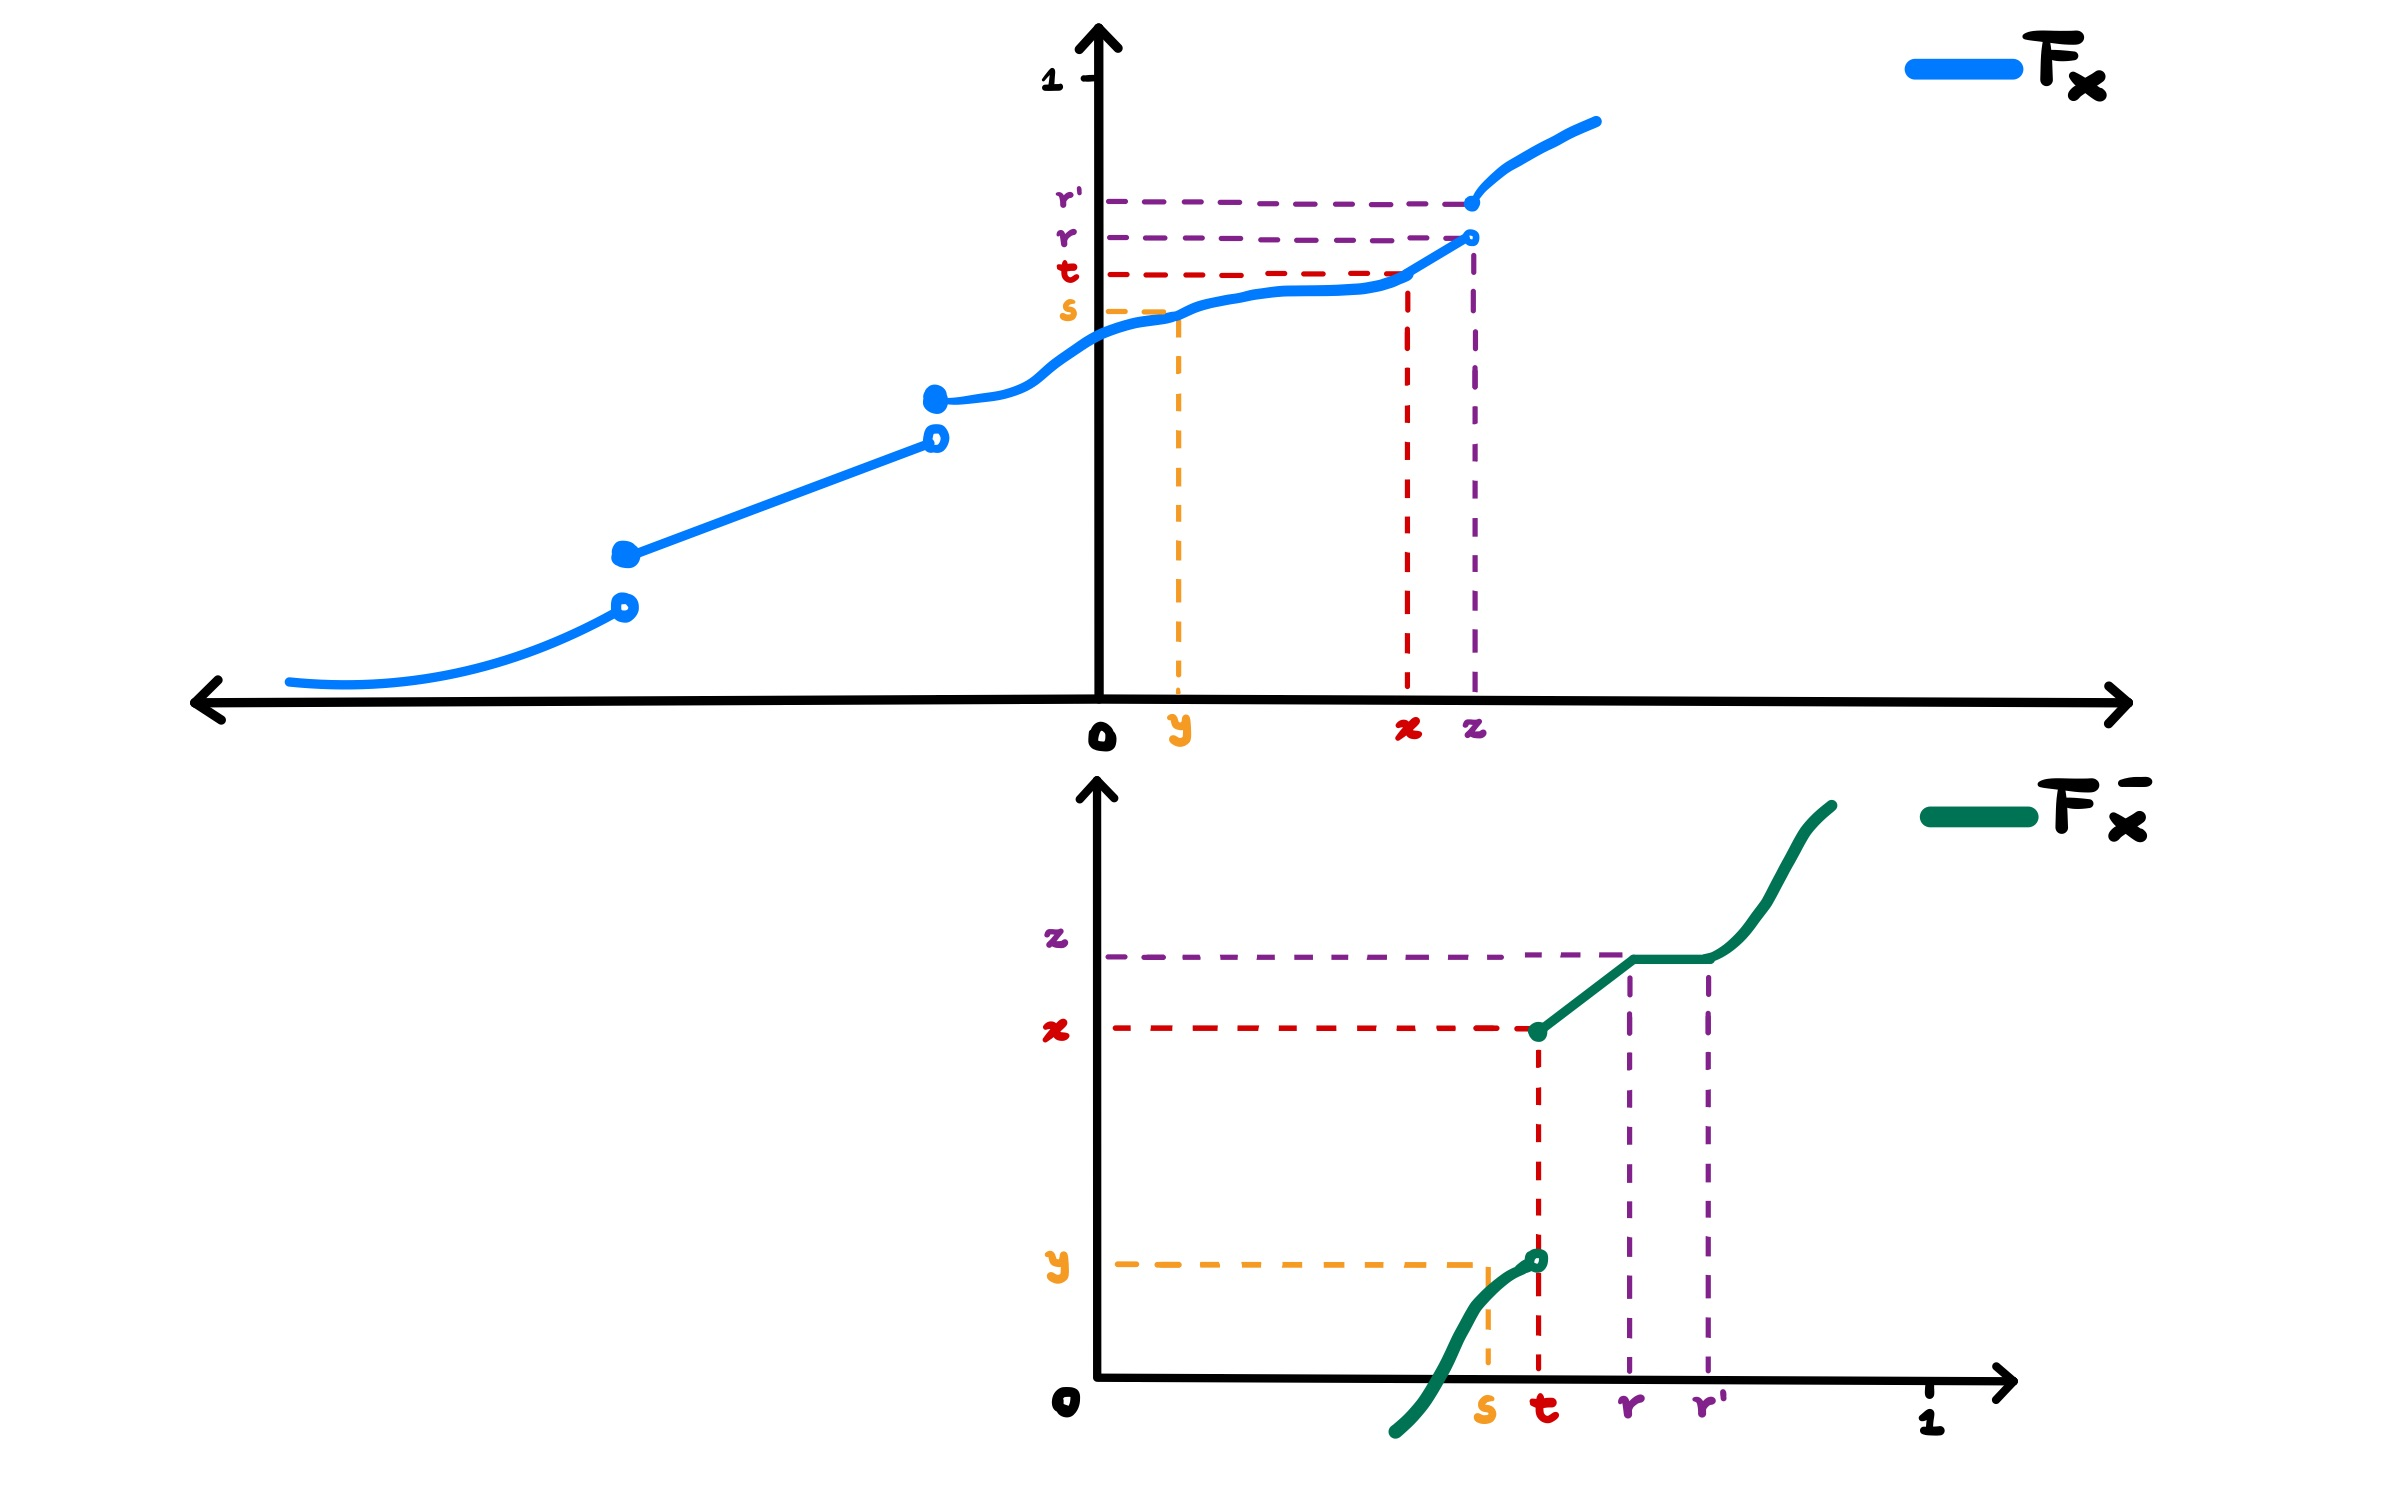
\includegraphics[scale=0.17]{img/clase_06_pag_10.jpg}
%     \caption{Ejemplo de inversa generalizada}
%     \label{fig:inv_gen}
% \end{figure}
\begin{images}[\label{fig:inv_gen}]{Ejemplo de inversa generalizada}
	\addimage{clase_06_pag_10_01}{width=11cm}{Función $F_X$}
	\imagesnewline
    \addimage{clase_06_pag_10_02}{width=10cm}{Función $F^-_{\mbox{ }X}$}
\end{images}

\vspace{1.5cm}\\
Veamos como se aplica el método de la inversa generalizada a las variables aleatorias \textbf{exponencial} y \textbf{Poisson}.

\begin{definition}[Variable exponencial]
Dado $\lambda>0$ la v.a. $X$ se dice exponencial si su densidad está dada por:
$$ f_X(x) = \lambda e^{-\lambda x}, \forall x\geq 0 \, ,$$
lo cual se denota $X\sim exp(\lambda)$.
\end{definition}

Sea la v.a. $X\sim exp(\lambda)$ con $\lambda>0$. Notemos que su función distribución está dada por \\ $F_X(x)=1-e^{-\lambda x}$. Luego por Proposición \ref{propinvgen},
$$\Finvgen(z)=\displaystyle\frac{-\ln(1-z)}{\lambda} \, .$$
Además, como tenemos $1-U\igualley U$, se sigue el siguiente corolario:
\begin{corolary}[Simulación de una exponencial con inversa generalizada]
\label{simexp}  %%
Sea la v.a. $X\sim exp(\lambda)$ con $\lambda>0$, entonces
% Sea la v.a. $X\sim exp(\lambda)$ con $\lambda>0$. Notemos que su función distribución está dada por \\ $F_X(x)=1-e^{-\lambda x}$. Luego por Proposición \ref{propinvgen}, 
$$X=\displaystyle\frac{-\ln(1-U)}{\lambda}\sim exp(\lambda) \, .$$
\end{corolary}

\begin{definition}[Distribución Poisson]
Dado $\lambda>0$ decimos que la v.a. $N$ posee distribución de Poisson de parámetro $\lambda$ si su función de distribución está dada por:
$$ \P(N=n)=\displaystyle\frac{e^{-\lambda}\lambda^n}{n!} \, .$$
\end{definition}
\begin{remark}
Recordemos que la distribución de Poisson aproxima el número de éxitos cuando repetimos muchas veces un experimento con probabilidad baja de éxito cada vez. Equivale al máximo $n\in\N$ tal que la suma de $n$ exponenciales no sume más que $\lambda$.
\end{remark}
Usando esto y el Corolario \ref{simexp} tenemos lo siguiente:
\begin{corolary}[Simulación de una Poisson con inversa generalizada]
Sean $(U_i)_{i\in\N} \, \iid$ y sea $\lambda>0$, entonces
$$ N = \sup\{n\in\N : \displaystyle - \sum^n_{i=1}\ln(U_i)<\lambda\}$$
% Sea $N$ distribución de Poisson, luego podemos simular $N$ como
tiene ley de Poisson de parámetro $\lambda$.
\end{corolary}
\subsubsection{Gaussianas}
Consideremos dos distribuciones Gaussianas independientes (ver definición \ref{gauss}). Para simularlas usaremos la transformada de Box-Muller:

\begin{proposition}[Método de Box-Muller] 
Sean $U,V\sim\unif$, definimos:
$$R:=\displaystyle\sqrt{-2 \ln U}\, ,$$ y $$ \hat{\theta}:=(cos(2\pi V),sen(2\pi V)) \, .$$
Luego tenemos
$$ X=(X_1,X_2):=R\hat{\theta}\sim\normal(0,I_2) \, .$$
O sea, $X_1\indep X_2$ y $X_1,X_2\sim\normal(0,1)$.
\end{proposition}
\begin{proof}
\ejercicio. \gris Indicación: usar teorema de cambio de variables en $\R^2$. \negro
\end{proof}

\subsubsection{Variables aleatorias discretas cualquiera}
\label{disc}
Queremos simular $X$ v.a. discreta que toma valores $x_1<x_2<x_3<\dots<x_n<\dots$ $n\in\N$.
\begin{proposition}
Sea $X$ v.a. discreta y $p_n=\P(X=x_n)$ su función de probabilidad. Definimos una partición de $[0,1]:0=a_0<a_1<\dots<a_n\leq1$ mediante $a_n=\sum_{k\leq n}p_k$. Entonces podemos simular $X$ usando
$$ Y:=\displaystyle\sum_{n\in\N}x_n \mathbf{1}_{a_{n-1},a_n}(U)\igualley X \, .$$
\end{proposition}
\begin{proof}
Basta ver que $Y=\Finvgen(U)$. \ejercicio
\end{proof}

\subsubsection{Caso inversa no explícita}
Sea $X$ variable aleatoria real con densidad $f_X$ estrictamente positiva. Entonces la función de distribución $F_X$ es derivable y estrictamente creciente. Si \textbf{no conocemos} $F_X$ %la inversa 
o no la podemos invertir, usaremos el siguiente método:
\begin{definition}[Aproximación de Newton-Raphson]
Dado $U\in[0,1]$ queremos encontrar el único $\bar{x}$ tal que $F_X(\bar{x})=U$ (de este modo $\bar{x}=\Finvgen(U)$). Es decir, buscamos la única raíz de $G(x)=F_X(x)-U$.
\newline Luego el método de Newton-Raphson consiste en tomar:
$$ x_n:=x_{n-1}-\displaystyle\frac{G(x_{n-1})}{G'(x_{n-1})}=x_{n-1}-\frac{(F_X(x_{n-1})-U)}{f_X(x_{n-1})}\conv \bar{x} \, ,$$
e iterar hasta que ($F_X(x_k)-U$)$\leq\delta$ para $\delta$ pequeño dado.
\end{definition}

\subsection{Método general}
\subsubsection{Aceptación-rechazo}
\label{metgen}
Supongamos que queremos simular v.a. $X$ en $E$ espacio medible, con densidad conocida $f$ con respecto a una medida $\lambda(dx)$ en $E$, y que existe $Y$ v.a. en $E$ con densidad $g$ con respecto a $\lambda$ tal que:
\begin{itemize}
    \item sabemos simular fácilmente $Y$
    \item $\exists K>0 \tq f(x)\leq Kg(x)\mbox{ } \forall x \tq g(x)>0$
\end{itemize}
Veremos a continuación que podemos simular $X$ usando una sucesión $\iid (Y_n,U_n)_{n\geq 1}$ con $Y_n\igualley Y$, $U_n\sim\unif$ y $Y_n\indep U_n$. La segunda condición nos dice que no es necesario que $g$ ``domine'' $f$, sin embargo lo haría si amplificamos por una constante $K$.
\newp Vamos a necesitar la función siguiente:  % , $\forall x \in E$, definimos
% $$ \alpha(x):=\displaystyle\frac{f(x)}{Kg(x)}\in[0,1] \, .$$ 
$$ \alpha(x) := \begin{cases} 
    \displaystyle\frac{f(x)}{Kg(x)}  & \mbox{ si }g(x)>0\\
    0 & \mbox{ si }g(x)\leq0  \, .
\end{cases}$$
% Notemos que si $g(x)>0$,  $\alpha(x)\in[0,1]$. %$\frac{f(x)}{Kg(x)}\in[0,1]$.
Notemos que $\alpha(x)\in[0,1]$. Además $\displaystyle\int f \lambda(dx)\leq K\int g\lambda(dx)$, luego $K\geq 1$.
% \newp Luego se tiene la siguiente proposición:
\begin{proposition}[Método de aceptación-rechazo]
Sea $E$ un espacio medible cualquiera. Consideramos $X$ v.a. en $E$ con densidad $f$ e $Y$ v.a. en $E$ con densidad $g$ de modo que $\exists K>0 \tq $
$$f(x)\leq Kg(x) \espacio \forall x\in \{z\in E \,|\,g(z)>0 \}$$
\newline Sea $N=\inf\{n\geq 1:U_n\leq \alpha(Y_n)\}$, entonces tenemos:
\begin{itemize}
    \item[(i)] $N\sim Geom(\frac{1}{K})$
    \item[(ii)] $Y_N\sim Ley(X)$
    \item[(iii)] $Y_N\indep N$
\end{itemize}
\end{proposition}
\begin{proof}
\gris 
\begin{alignat*}{2}
    \P(Y_N\in A, N=m) & = \P(Y_m\in A, U_m \leq \alpha(Y_m),U_k>\alpha(Y_k),k=1,\dots,m-1) \\
     & = \P(Y_m\in A,U_m\leq \alpha(Y_m))(1-p)^{m-1} %\, .
     % \\ & = \displaystyle \int_A(\int^{\alpha(y)}_0 dt)g(y)\lambda(dy)(1-p)^{m-1}
     \\&  = \displaystyle \int_A \left(\int^{\alpha(y)}_0 dt\right)g(y)\lambda(dy)(1-p)^{m-1}
     \\ & = \frac{1}{K}\int_Af(y)\lambda(dy)(1-p)^{m-1} \, ,
\end{alignat*}
donde $p=\P(U_1\leq\alpha(Y_1))$. Luego tomando $A=E$ obtenemos
\begin{alignat*}{2}
    \P(N=m) & = \P(U_m \leq \alpha(Y_m))(1-p)^{m-1} \\
     & = p(1-p)^{m-1}
     \\ & = \frac{1}{K}(1-p)^{m-1} \, .
\end{alignat*}
Luego $p=\P(U_m\leq \alpha(Y_m))=\frac{1}{K}$, y $\therefore \espacio N\sim Geom(p)=\frac{1}{K}$.
\\ Así,
\begin{alignat*}{2}
    \P(Y_N\in A, N=m) & = \displaystyle \int_A f(y)\lambda(dy) p(1-p)^{m-1} \\
     & = \P(X\in A)p(1-p)^{m-1}
     \\ & =  \P(X\in A)\P(N=m) \, .
\end{alignat*} 
Sumando sobre $m\geq 1$ nos queda que
$$ \P(Y_N\in A) = \P(N=m)$$
Por ende $Y_n \igualley x$.
\\ Finalmente,
$$ \P(Y_N\in A, N=m) = \P(Y_N\in A)\P(N=m) $$
$\therefore \espacio Y_N\indep N$
\findem \negro
\end{proof}
% \vspace{.5cm}
\begin{remark}
\beforeitemize
\begin{itemize}
    \item Para obtener una realización de una v.a. de $Ley(X)$ se requiere simular una cantidad $N$ finita, pero aleatoria $\sim Geom(\frac{1}{K})$ (desconocida a priori) de pares $(Y_1,U_1),\dots,(Y_n,U_n),\dots$.
    \newline De ahí el nombre del método aceptación rechazo, pues si se cumple la condición aceptamos y si no rechazamos.
    \item $N\sim Geom(\frac{1}{k}) \implies \E(N)=K$. Luego, mientras más pequeño sea $K\geq 1$ tal que $f(x)\leq Kg(x)$, mejor, pues aceptamos el valor $Y_m$ más pronto.
    \item $K$ pequeño significa que g está más ajustada a $f$. Idealmente nos gustaría $K=1$, pero en ese caso tendríamos $0\leq g(x)-f(x)\implies 0\leq\int|g-f|\lambda(dx)=1-1=0\implies g\equiv f$ o sea, $X\igualley Y$. Si tuviésemos esto entonces ``ya sabríamos simular $X$'' ($Y$ es una v.a. que sabemos simular fácilmente).
\end{itemize}
\end{remark}

\subsubsection{Simulación condicional a subconjunto}
Como aplicación tenemos el siguiente corolario, donde \textbf{no necesitamos simular las uniformes}:
\begin{corolary}[Simulación de una v.a. $Y$  ``condicional a que $Y\in A$'']
\label{corclase7}
\newline Sean $(Y_n)_{n\geq 1}$ réplicas $\iid$ (simulables) de una v.a. $Y$ en $E$ y $A\subset E$. Sea $N:=\inf\{n\geq 1: Y_n\in A\}$, entonces
$$ \hat{Y}:=Y_N\sim Ley(Y|Y\in A) \espacio \mbox{ y }\espacio Y_N\indep N \, .$$
\end{corolary}
\begin{proof}
\gris
$X\sim Ley(Y|Y\in A)$ tiene densidad $f$ con respecto a $\lamnda=Ley(Y)$, dada por
$$ f(x) = K\mathbf{1}_A(x) = \P(Y\in A)^{-1}\mathbf{1}_A(x)\leq K g(x) \, ,$$
con $g\equiv 1$ la densidad $Y$ con respecto a $\lambda$.  Por el método aceptación-rechazo, $Y_N\sim Ley(Y|Y\in A)$, para $N=\inf\{n\geq1:U_n\leq\alpha(Y_n)\}$, donde $(U_n)_{n\in\N}\indep (Y_n)_{n\geq1}$ son $\iid$ y distribuyen $\unif$. Pero $U_n\leq\alpha(Y_n)=\mathbf{1}_A(Y_n)\Longleftrightarrow Y_n\in A$
\findem
\negro
\end{proof}

% \begin{proposition}[Caso particular de Corolario \ref{corclase7}]
\subsection{Variables condicionadas a estar en un intervalo}
\begin{proposition}
Consideramos $X$ una v.a. real cualquiera y $A=[a,b]$. Sea $V\sim\mathbb{U}([F_X(a),F_X(b)])$.
Notemos que 
$$V\igualley F_X(a)+U(F_X(b)-F_X(a))$$
con $U\sim \unif$. Entonces
$$ \Finvgen (V) \sim Ley(x \, |\, x\in[a,b]) \, .$$
\end{proposition}
\begin{proof}
\ejercicio
\newline \gris Indicación: demostrar y utilizar: $F_{\{x|x\in[a,b]\}}(x)=\displaystyle\frac{F_X(x)-F_X(a)}{F_X(b)-F_X(a)}$. \negro
\end{proof}
% \vspace{1cm}
\subsection{Técnicas de reducción de varianza en M.M.C}
Para una presentación sucinta de estos temas ver el capítulo 1 del libro \textit{Processus de Markov et applications. Algorithmes, Réseaux, Génome et
Finance}, capítulo 1, É. Pardoux \cite{pardoux} y con el algo más de profundidad \textit{Monte -Carlo methods in financial engineering} de P. Glasserman, capítulo 1. Para más detalles ver Asmussen ``Stochastic Simulation'' \cite{asm}.
\newp \textbf{Idea}: si disponemos de $Y_1,\dots,Y_n,\dots \iid$ para aproximar $I=\E(Y)$, el error cometido será menor si $\sigma^2=\var(Y)$ es menor (para igual $\E(Y)$).
\begin{itemize}
    \item $\E(|\bar{Y}_n-I|^2)=\displaystyle\frac{\var(Y)}{n}$
    \item con un nivel de confianza $\alpha\in(0,1)$ dado, $\P(|\bar{Y}_n-I|<\epsilon)\gtrsim 1-\alpha$ si $n\geq\nmc$
\end{itemize}
Luego si podemos simular $Y'_1,\dots,Y'_n$ tal que $\E(Y')=I$ y $\var(Y')<\var(Y)$ (a costo comparable), necesitaremos menos ``$n$''s y seremos más eficientes.
\newp Los métodos de reducción de varianza que veremos son los siguientes:
\begin{enumerate}
    \item Variable de control (\ref{control})
    \item Variables antitéticas (\ref{antitéticas})
    \item Muestreo preferencial (\ref{preferencial})
    \item Muestreo estratificado (\ref{estratificado})
\end{enumerate}
Notar de todos modos que para comparar dos métodos de calcular $I=\E(Y)$, de todas maneras hay que considerar el costo ``por réplica''.

\subsubsection{Variable de Control}
\label{control}
Supongamos que podemos simular $Y=f(X)$ y que conocemos $\E(h(X))$ explícitamente para cierta función real $h$, que llamaremos  \textbf{variable de control}.
\newp Disponemos entonces de muchos ``estimadores'' de $I$ ``posibles'': para cada $c\in\R$,
$$ \sumfx+c\mbox{ }[\frac{1}{n}\sum_{k=1}h(X_k)-\E(h(X))] 
 =\frac{1}{n}\sum_{k=1}^n[f(X_k)+c(h(X_k)-\E(h(X))]
 =\frac{1}{n}\sum^n_{k=1}\varphi_c(X_k) \, ,$$
con $\E(\varphi_c(X_1))=I$.\hspace{.3cm} ¿Cual es su varianza?
\begin{alignat*}{2}
    \var(\varphi_c(X_1)) & = \var(f(X_1)+ch(X_1)) \\
     & = \var(f(X_1))+c^2\var(h(X_1))+2\mbox{ }c\mbox{ }Cov(h(X_1),f(X_1)) \, .
\end{alignat*}
% $$ \var(\varphi_c(X_1))=\var(f(X_1)+ch(X_1)) = \var(f(X_1))+c^2\var(h(X_1))+2\mbox{ }c\mbox{ }Cov(h(X_1),F(X_1))$$
De lo anterior se desprende que la varianza disminuye cuando se cumple:
$$ c^2 Var(h(X)) + 2c Cov(h(X),f(X)) < 0 $$

Además podemos optimizar en $c\in\R$. Queda:
$$ c^*=\displaystyle\frac{-Cov(f(X_1),h(X_1))}{\var(h(X_1))} \, .$$
%i.e., hacemos que los dos términos finales se cancelen. Así quedará sólo la varianza de $f(X_1)$. 
Substituyendo arriba:
$$ \var(\varphi_{c^*}(X_1))=\sigma^2-\displaystyle\frac{Cov(f(X_1,h(X_1)))^2}{\var(h(X_1))} \, .$$
Luego $\var(\varphi_{c^*}(X_1))<\sigma^2$ si $Cov(f(X_1,h(X_1))\neq 0$, i.e., reducimos la varianza del estimador.
\newp En general, quizás no conocemos $Cov(f(X_1,h(X_1))$ ni $\var(h(X_1))$. Pero los podemos estimar con $q$ (pequeño) simulaciones ``piloto''. Primero, usando la Ley de grandes números tenemos que,
$$ \displaystyle\frac{\sum_{k=1}^q(Y_k-\bar{Y}_q)(Z_k-\E(Z_1))}{q-1} \mbox{ }\substack{\longrightarrow \\ q\to\infty}\mbox{ } Cov(Y_1,Z_1) \, ,$$
entonces
$$ Cov(f(X_1,h(X_1)))\approx \displaystyle\frac{\sum_{k=1}^q(Y_k-\bar{Y}_q)(Z_k-\E(Z_1))}{q-1} \, ,$$
con $Y_k=f(X_k),Z_k=h(X_k)$ y 
$$\var(h(X_1))\approx \displaystyle\frac{\sum_{k=1}^q(Z_k-\E(Z_k))^2}{q-1} \, ,$$
luego,
$$ \hat{c}^*=\displaystyle\frac{\sum_{k=1}^q(Y_k-\bar{Y}_q)(Z_k-\E(Z_1))}{\sum_{k=1}^q(Z_k-\E(Z_k))^2} \, ,$$
y aproximaremos entonces $I$ mediante el siguiente promedio empírico:
$$ \displaystyle \frac{1}{n}\sum^q_{k=1}[f(X_k)-\hat{c}^*(h(X_k))-\E(h(X_1))]=\frac{1}{n}\sum^q_{k=1}\hat{\varphi}(X_k) \, .$$
\begin{example}[Ejemplo ``juguete'' de aplicación de variable de control]
Queremos calcular $I=\int^1_0e^xdx$ (ya sabemos que esto vale $e-1$).
\newp Método ``usual'': $I=\E(f(X))=\E(e^X),X\sim \unif$ donde $\var=\var(e^X)\approx0,242$
\newp Por otro lado, considerando $h(X_1)=\int^1_0(x+1)dx$ como variable de control:
$$ I=\int^1_0e^xdx - (\int^1_0(x+1)dx-\frac{3}{2})=\int^1_0(e^x-1-x)dx+\frac{3}{2} \, .$$
Tomando $c=-1,h(X)=x+1$. En este caso se puede verificar que:
$$ \var(e^X-1-x)\approx0.00437 \, .$$
Esto es 5 veces menos que $Var(e^X)$.
\end{example}

\subsubsection{Variables antitéticas (de a pares)}
\label{antitéticas}
Sea $I=\E(Y)$ con \hspace{.2cm} $Y=f(X)$ y \hspace{.2cm} $X$ v.a. en $\R$. Consideremos el M.M.C usual usando $(X_n)_{n\geq1}\iid \sim Ley(x)$, con $\var(f(x))=\sigma^2$. Para un número par $2n$ de réplicas $Y_k=f(X_k)$, $\bar{Y}_{2n}=\frac{1}{2n}(Y_1+\dots+Y_{2n})\conv I$ con $ECM_{2m}=\E(|\bar{Y}_{2n}-I|^2)=\displaystyle\frac{\sigma^2}{2n}$ (error cuadrático medio).
\newp Supongamos que simultáneamente podemos simular $(X_n')_{n\geq 1}\sim Ley(X)$ de modo que $X_n$ y $X_n'$ están \textbf{correlacionadas}, y la sucesión de pares $(X_n,X_n')_{n\geq1}$ son $\iid$ (independiente de los anteriores). Entonces también:
$$ \displaystyle\frac{1}{2}(\bar{Y}_n+\bar{Y}_n')=\frac{1}{2n}[(Y_1+Y_1')+\dots+(Y_n+Y_n')]\conv I\, .$$
\textbf{¿Con qué $ECM'_{2m}$?}
\newline $\displaystyle\frac{1}{2}(\bar{Y}_n+\bar{Y}_n')=\frac{1}{n}\sum^n_{k=1}\frac{(Y_k+Y_k')}{2}$ con $\frac{Y_k+Y_k'}{2}=\frac{f(X_k)+f(X_k')}{2},\mbox{ } k\geq1\mbox{ }\iid$ de media $\E(f(X))=I$.
\begin{alignat*}{2}
ECM_2n' & = \E\bigg(\bigg|\frac{1}{2}(\bar{Y}_n+\bar{Y}_n'-I)\bigg|^2\bigg) \\
& =\frac{1}{n}\var\bigg(\frac{Y_1+Y_1'}{2}\bigg) \\
& =\frac{1}{4n}[2\var(Y_1)+2\cov(Y_1,Y_1')] \\
& =\frac{1}{2n}(\sigma^2+\cov(f(X_1),f(X_1')))
\end{alignat*}
% $$ECM_2n'=\E(|\frac{1}{2}(\bar{Y}_n+\bar{Y}_n'-I)|^2)=\frac{1}{n}\var(\frac{Y_1+Y_1'}{2})=\frac{1}{4n}[2\var(Y_1)+2\cov(Y_1,Y_1')]=\frac{1}{2n}(\sigma^2+\cov(f(X_1),f(X_1')))$$
Luego si $\cov(f(X_1),f(X_1'))<0$, $$ECM'_{2n}<\frac{\sigma^2}{2n}=ECM_{2n} \, .$$
Aplicación usual: $X_n=U_n\sim\unif$, $X_n'=1-U_n\sim\unif$ (la realización $U_n$ es la misma para $X$ y $X'$), y las $2n$ variables aleatorias $U_1,\dots,U_n$, $1-U_1,\dots1-U_n$ requieren solo $n$ simulaciones.
\newp \textbf{¿Cuando se tiene $\cov(f(U_1),f(1-U_1))\leq 0$?}
Respondemos esto con el siguiente lema.
\begin{lemma}
Sea $f:[0,1]\to\R$ función monótona tal que $f\in L^2([0,1],dx)$. Entonces $\cov(f(U),f(1-U))\leq0$.
\end{lemma}
\begin{proof}  % 10:40
\gris
Sea $\tilde{U}\sim \unif$, $\tilde{U}\indep U$. Para $f$ creciente o decreciente siempre tenemos
$$ (f(U)-f(\tilde{U}))(f(1-U)-f(1-\tilde{U})) \leq 0 \, .$$
Tomando la esperanza se tiene que
$$ 2(\E(f(U)f(1-U))-\E(f(U))\E(f(1-\tilde{U})))\leq 0 $$
$$ \Longleftrightarrow \E(f(U)f(1-U))-\E(f(U))^2 \leq 0 \, .$$
\findem
\negro
\end{proof}

\textbf{Receta general}: Luego si tenemos $f:[0,1]\to\R$ monótona (por ejemplo $f=F^-_{\mbox{ }Z}$ una función de distribución inversa) usando $n$ réplicas $\unif$, el estimador: $$\displaystyle\frac{1}{n}\sum^n_{k=1}[\frac{f(U_k)+f(1-U_k)}{2}]$$ aproxima $I=\E(f(U))$ con varianza menor a $\sigma^2/2n$, es decir, menos de la mitad de la varianza $\sigma^2/n$ del estimador usual: $$\displaystyle\frac{1}{n}\sum^n_{k=1}f(U_k)$$ construido con las mismas $n$ réplicas.
%\textbf{Receta general}: cuando tengamos $f$ función monótona aplicada a una uniforme $U$, entonces en vez de usar
%$$\displaystyle\frac{1}{n}\sum^n_{k=1}f(U_k)$$
%Usamos $$\displaystyle\frac{1}{n}\sum^n_{k=1}[\frac{f(U_k)+f(1-U_k)}{2}] $$
%Y reduciremos la varianza a la mitad.
\vspace{1cm}\\
\subsubsection{Muestreo preferencial (\textit{importance sampling})}
\label{preferencial}
Queremos calcular $I=\E(f(X))=\int f(x)\mu(dx)$ con $X\sim \mu$ y supongamos que podemos simular $Z\sim\nu$ simulable tal que $\nu\approx\mu$ .  % con $Z\sim \nu$ simulable. 
Es decir $\exists L:\R^d\to\R_+$ densidad de Radon-Nikodym tal que $\nu(dx)=L(x)\mu(dx)$ con $L>0$ $\mu-c.s.$,
\newline Entonces 
$$I=\displaystyle\int\frac{f(x)}{L(x)}\nu(dx)\, ,$$ 
y podemos calcular $I$ también como 
$$I=\displaystyle\E\left(\frac{f(Z)}{L(Z)}\right) \, .$$
\textbf{¿Podemos encontrar $\nu$ así, de manera que además $\var(\frac{f(Z)}{L(Z)})<\var(f(X))$?}
\begin{remark}
\begin{alignat*}{2}
    \var\left(\displaystyle\left(\frac{f(Z)}{L(Z)}\right)\right) & = \E\left(\frac{f(Z)^2}{L(Z)^2}\right)-I^2\\
     & = \int \frac{f(z)^2}{L(z)^2}\mu(dz) - [\int f(x)\mu(dx)]^2 \\
     & = \int \frac{|f(z)|}{L(z)}\frac{|f(z)|}{L(z)}\mu(dz) - [\int f(x)\mu(dx)]^2 \\
     & = \int |f(z)|\frac{|f(z)|}{L(z)}\mu(dz) - [\int f(x)\mu(dx)]^2 \, .
\end{alignat*}
\end{remark}
Si $f\geq0$, tomando $L(z)=\displaystyle\frac{f(Z)}{I}$, o sea $\nu(dz)=\displaystyle\frac{f(Z)}{I}\mu(dz)$ y obtendríamos 
$$\var\left(\frac{f(Z)}{L(Z)}\right)=0 \, ,$$
pues $\frac{f(Z)}{L(Z)}=I$.
% \begin{remark}
\newp Lo anterior no se puede usar en la práctica porque \textbf{no conocíamos $I$}. Pero la fórmula $\nu(dz)=\frac{f(Z)}{I}\mu(dz)$ nos sugiere que sirve samplear de una ley parecida a $\mu$ (y equivalente) pero que da más peso a puntos $z$ tales que $f(z)$ es más grande, o sea que son \textbf{más importantes} en el cálculo de $\int f(x)\mu(dx)$.
% \end{remark}
\newp \textbf{Heurística}:
\begin{itemize}
    \item Buscar una medida $\tilde{\nu}$ ``parecida a $|f(x)|\mu(dx)$''
    \item Esta medida debe cumplir que $\nu(dx):=\displaystyle\frac{\tilde\nu(dx)}{\int\tilde{\nu}(dx)}$, sea ``\textbf{fácilmente simulable}'' donde $\int\tilde{\nu}(dx)$ es una constante de normalización calculable. 
\end{itemize}
\begin{example}[Aplicación ``artificial'' de muestreo preferencial]
Queremos aproximar $$I=\displaystyle\int^1_0\cos(\frac{\pi x}{2})dx=\frac{2}{\pi} \, ,$$ con $\mu(dx)=dx$ uniforme en $[0,1]$, $f(x)=\cos(\frac{\pi x}{2})$.\\
\newline Elegimos $\nu(dz)=\frac{z}{2}(1-z^2)dz=L(z)dz$ y aproximamos
$$ I\approx\displaystyle\frac{1}{n}\sum^n_{k=1}\cos(\frac{\pi z_k}{2})/L(z_k), \espacio Z_k \iid \sim \nu \, .$$
En la figura \ref{fig:pref} se grafican ambas funciones. Se puede mostrar que la varianza se reduce en factor mayor que $10$.
\begin{figure}
    \centering
    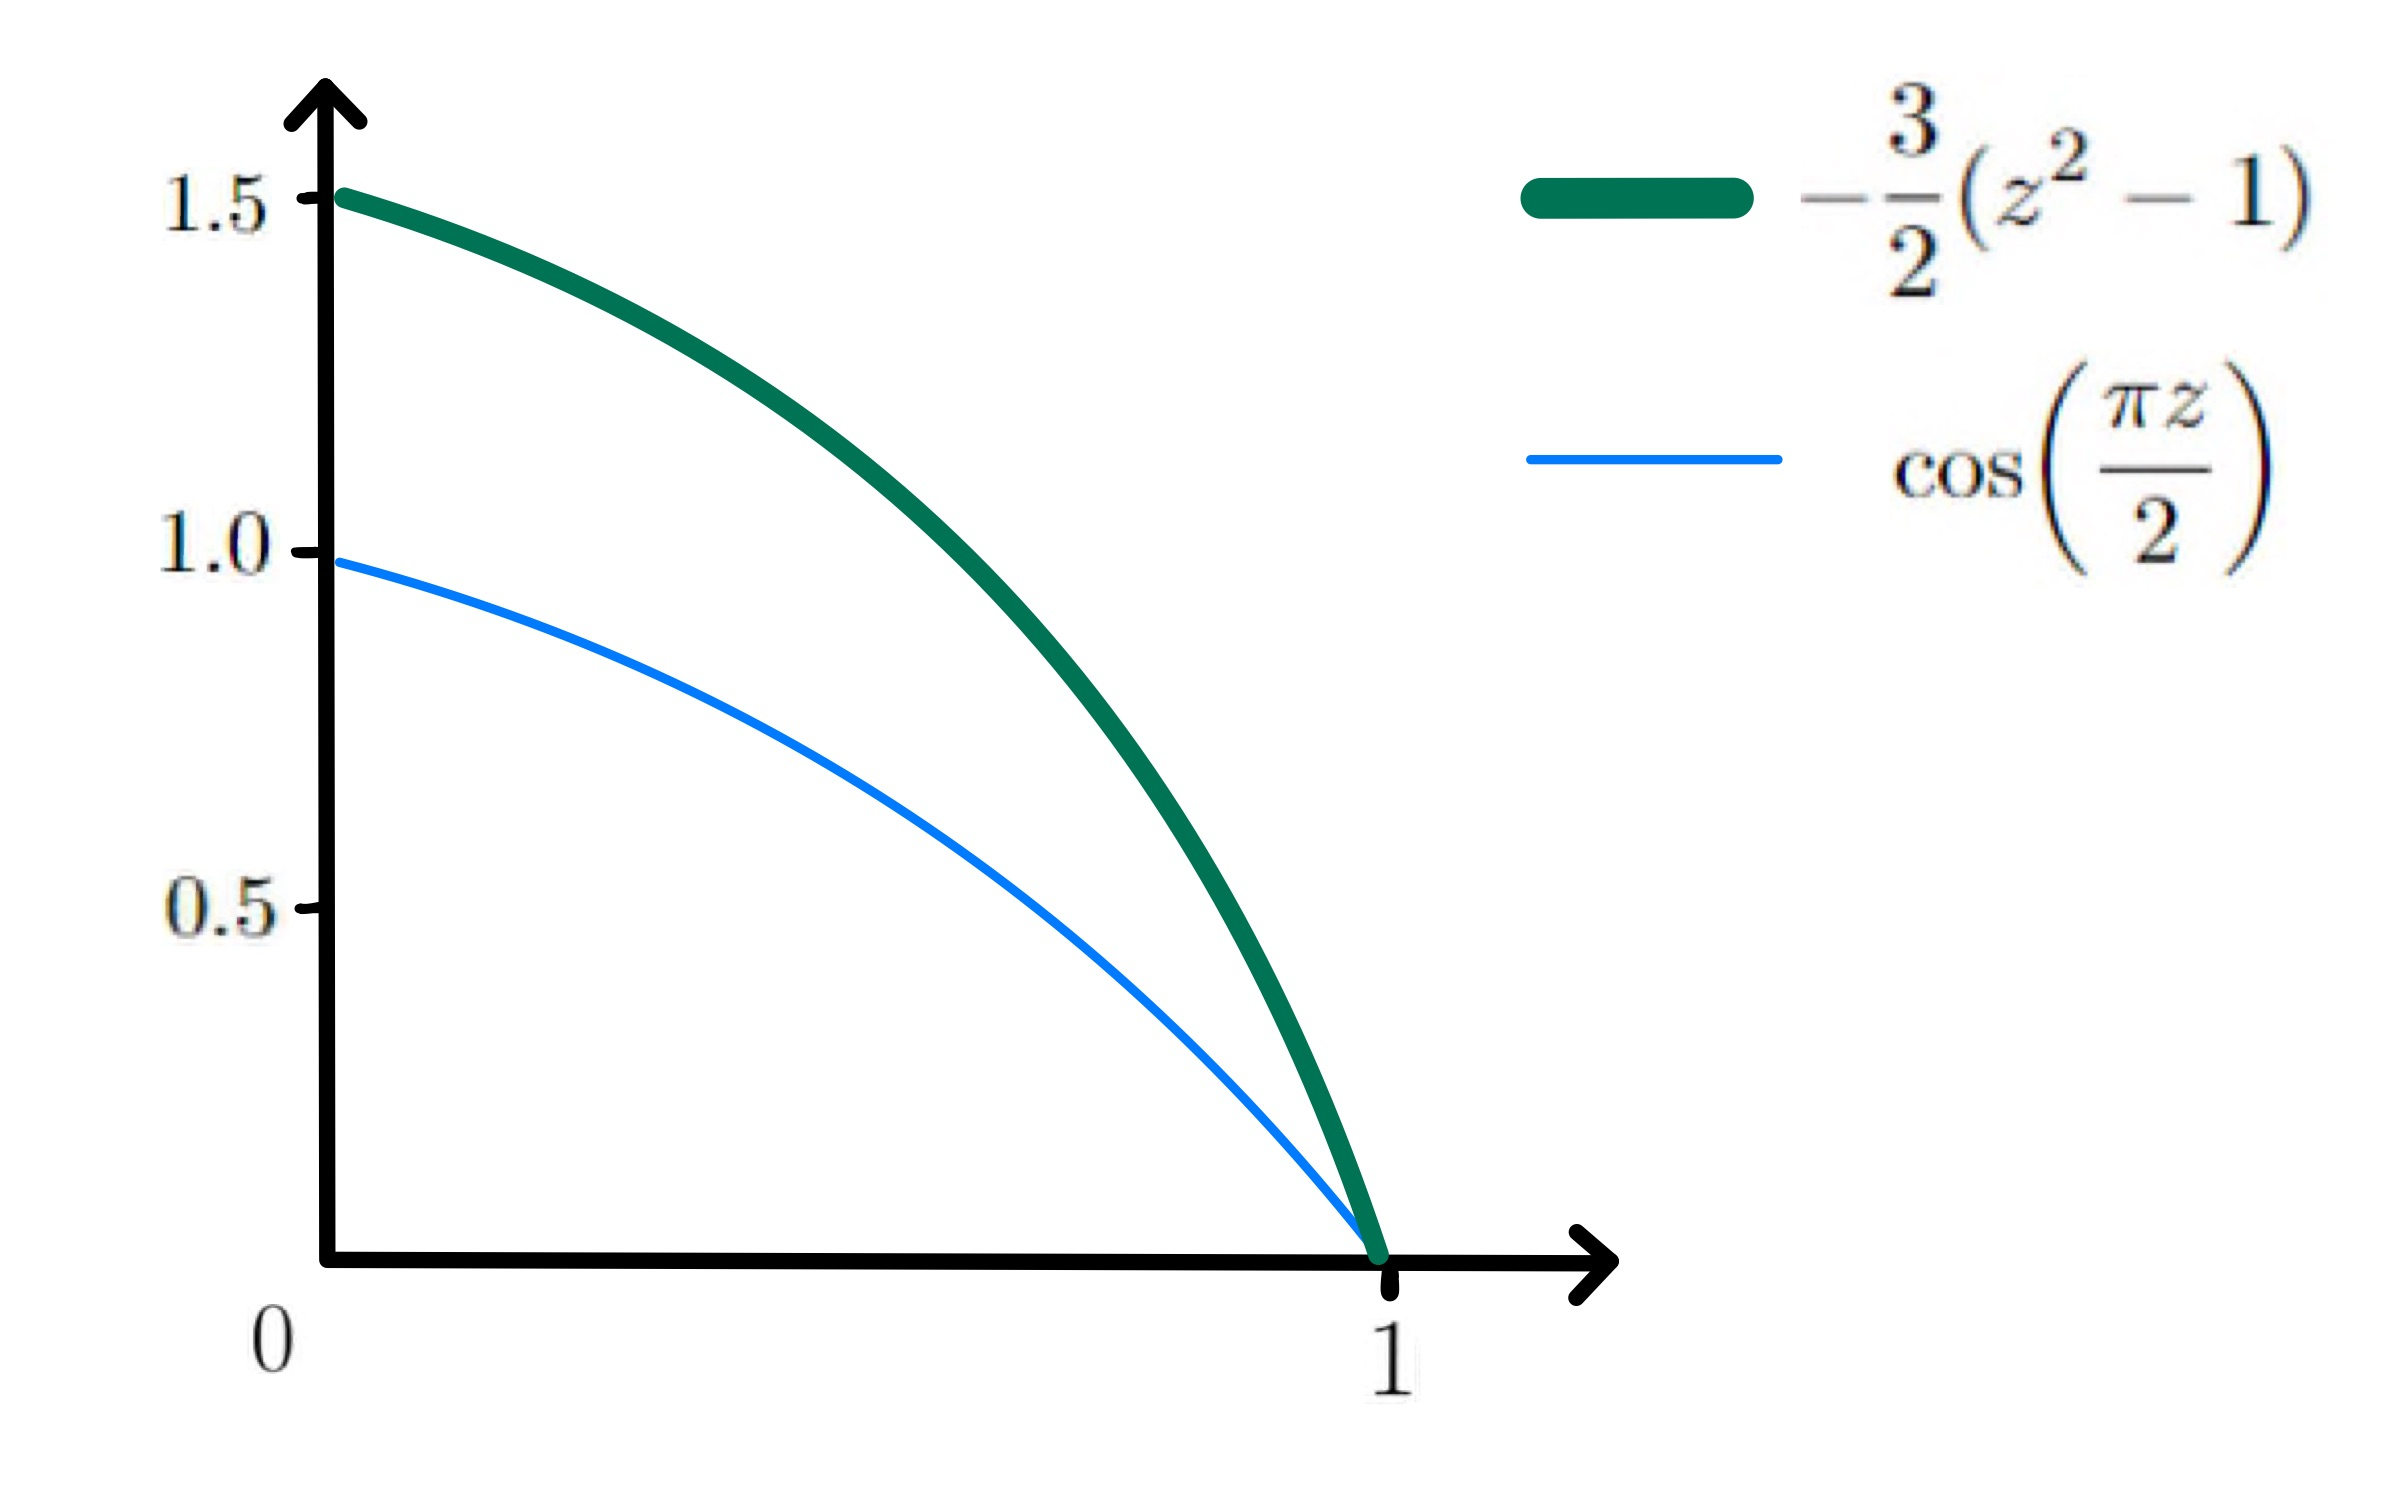
\includegraphics[scale=0.11]{img/clase_08_pag_11.jpg}
    \caption{Ejemplo de muestreo preferencial}
    \label{fig:pref}
\end{figure}
% \begin{images}[\label{fig:pref}]{Ejemplo de muestreo preferencial}
%     \addimage{clase_08_pag_11}{width=10cm}{}
% \end{images}
\end{example}

\subsubsection{Muestreo estratificado (\textit{stratified sampling})}
\label{estratificado}
Queremos calucular $I=\E(Y), Y$ v.a. $\in\R$ con $\sigma^2=\var(Y)$. 
\newline Supongamos que tenemos una partición $\mathcal{D}=\{D_1,\dots,D_k\}$ (``estratos'') de $\R$, conocemos \\ $p_i=\P(Y\in D_i)$, y sabemos simular $Y^j\sim Ley(Y | Y \in D_j)$ para cada $j=1,\dots,k$.
\begin{example}
En $\R$, $D_j$ de la forma $[a_j,b_j)$, vimos como simular $Y^j$ usando $F_Y^-$ y una v.a. $U[f_Y(a_j),f_X(b_j)]$.
\end{example}
Disponemos entonces de:
$$ n=n_1+\dots+n_k \mbox{ v.a. independientes }:\begin{cases}
Y^1_1,\dots,Y^1_{n_1} \iid \igualley Y^1 &\\
\dots & \\
Y^k_1,\dots,Y^k_{n_k} \iid \igualley Y^k &
\end{cases} $$
\textbf{¿Podemos estimar $I$ con $\var<\displaystyle\frac{\sigma^2}{n}=\var\left(\frac{1}{n}\sum^k_{j=1}Y_j\right)$ con $(Y_n)\igualley Y \iid$?}
Para responder a esto notemos que
\begin{alignat*}{2}
    \E(Y) & = \E(\E(Y|K)) \mbox{ con }K=j \mbox{ ssi }Y\in D_j\\
     & = \displaystyle\E(\sum^k_{j=1}\E(Y|K=j)\mathbf{1}_{k=j}) \\
     & = \displaystyle\sum^k_{j=1}p_j\E(Y^j) \, .
\end{alignat*}
Definimos
$$ \hat{Y}_n=\displaystyle\sum^k_{j=1}p_j\frac{1}{n_j}\sum^{n_j}_{i=1}Y^j_i \, .$$
\begin{remark}
\beforeitemize
\begin{itemize}
    \item $\E(\hat{Y}_n)=I$, es decir, $\hat{Y}_n$ que es un estimador insesgado de $I$.
    \item $\hat{Y}_n\to I$ c.s.  cuando  $n_1, \dots, n_k\to \infty $ con   $n=n_1+ \dots + n_k $, por Ley de Grandes N\'umeros. 
\end{itemize}
\end{remark}
% \begin{proof}
% \gris Probar que son insesgados y usar ley de grandes números en cada estrato. (\ejercicio)\negro
%\end{proof}
\textbf{¿Con qué ECM (varianza)?}
\newline Usando la independencia de las v.a.  $Y_{k}^j$,  tenemos: % En general:
$$ \var(\hat{Y}_n)=\displaystyle\frac{1}{n}\sum^k_{j=1}\frac{p_j^2}{n_j}\sigma^2_j \, .$$
Veamos que esto es menor que $\sigma^2/n$ \, . Usaremos la
\begin{proposition}[Fórmula de la ``varianza total'']
Sea $Y$ v.a. real y $K$ v.a. cualquiera, luego
$$ \var(Y)=\E(\var(Y|K))+\var(\E(Y|K)) \, .$$
Donde $\E(\var(Y|K))=\E((Y-\E(Y|K))^2|K)$.
\end{proposition}
\begin{proof}
\ejercicio
\end{proof}
Entonces aplicando lo anterior a  la v.a. $K$ definida como $K=j$ cuando $Y\in D_j$, obtenemos:
$$ \sigma^2\,=\,\displaystyle\sum^k_{j=1}p_j\sigma^2_j+\sum^k_{j=1}p_j(\E(Y^j)-\E(Y))^2\,\geq \,\sum^k_{j=1}p_j\sigma^2_j \, .$$
Aqu\'i, por un lado $\sum^k_{j=1}p_j\sigma^2_j$ corresponde a la esperanza de la varianza condicional, mientras que el término $\sum^k_{j=1}p_j(\E(Y^j)-\E(Y))^2$ es la varianza de la esperanza condicional (ver Figura \ref{fig:estrat}). 
\begin{figure}
    \centering
    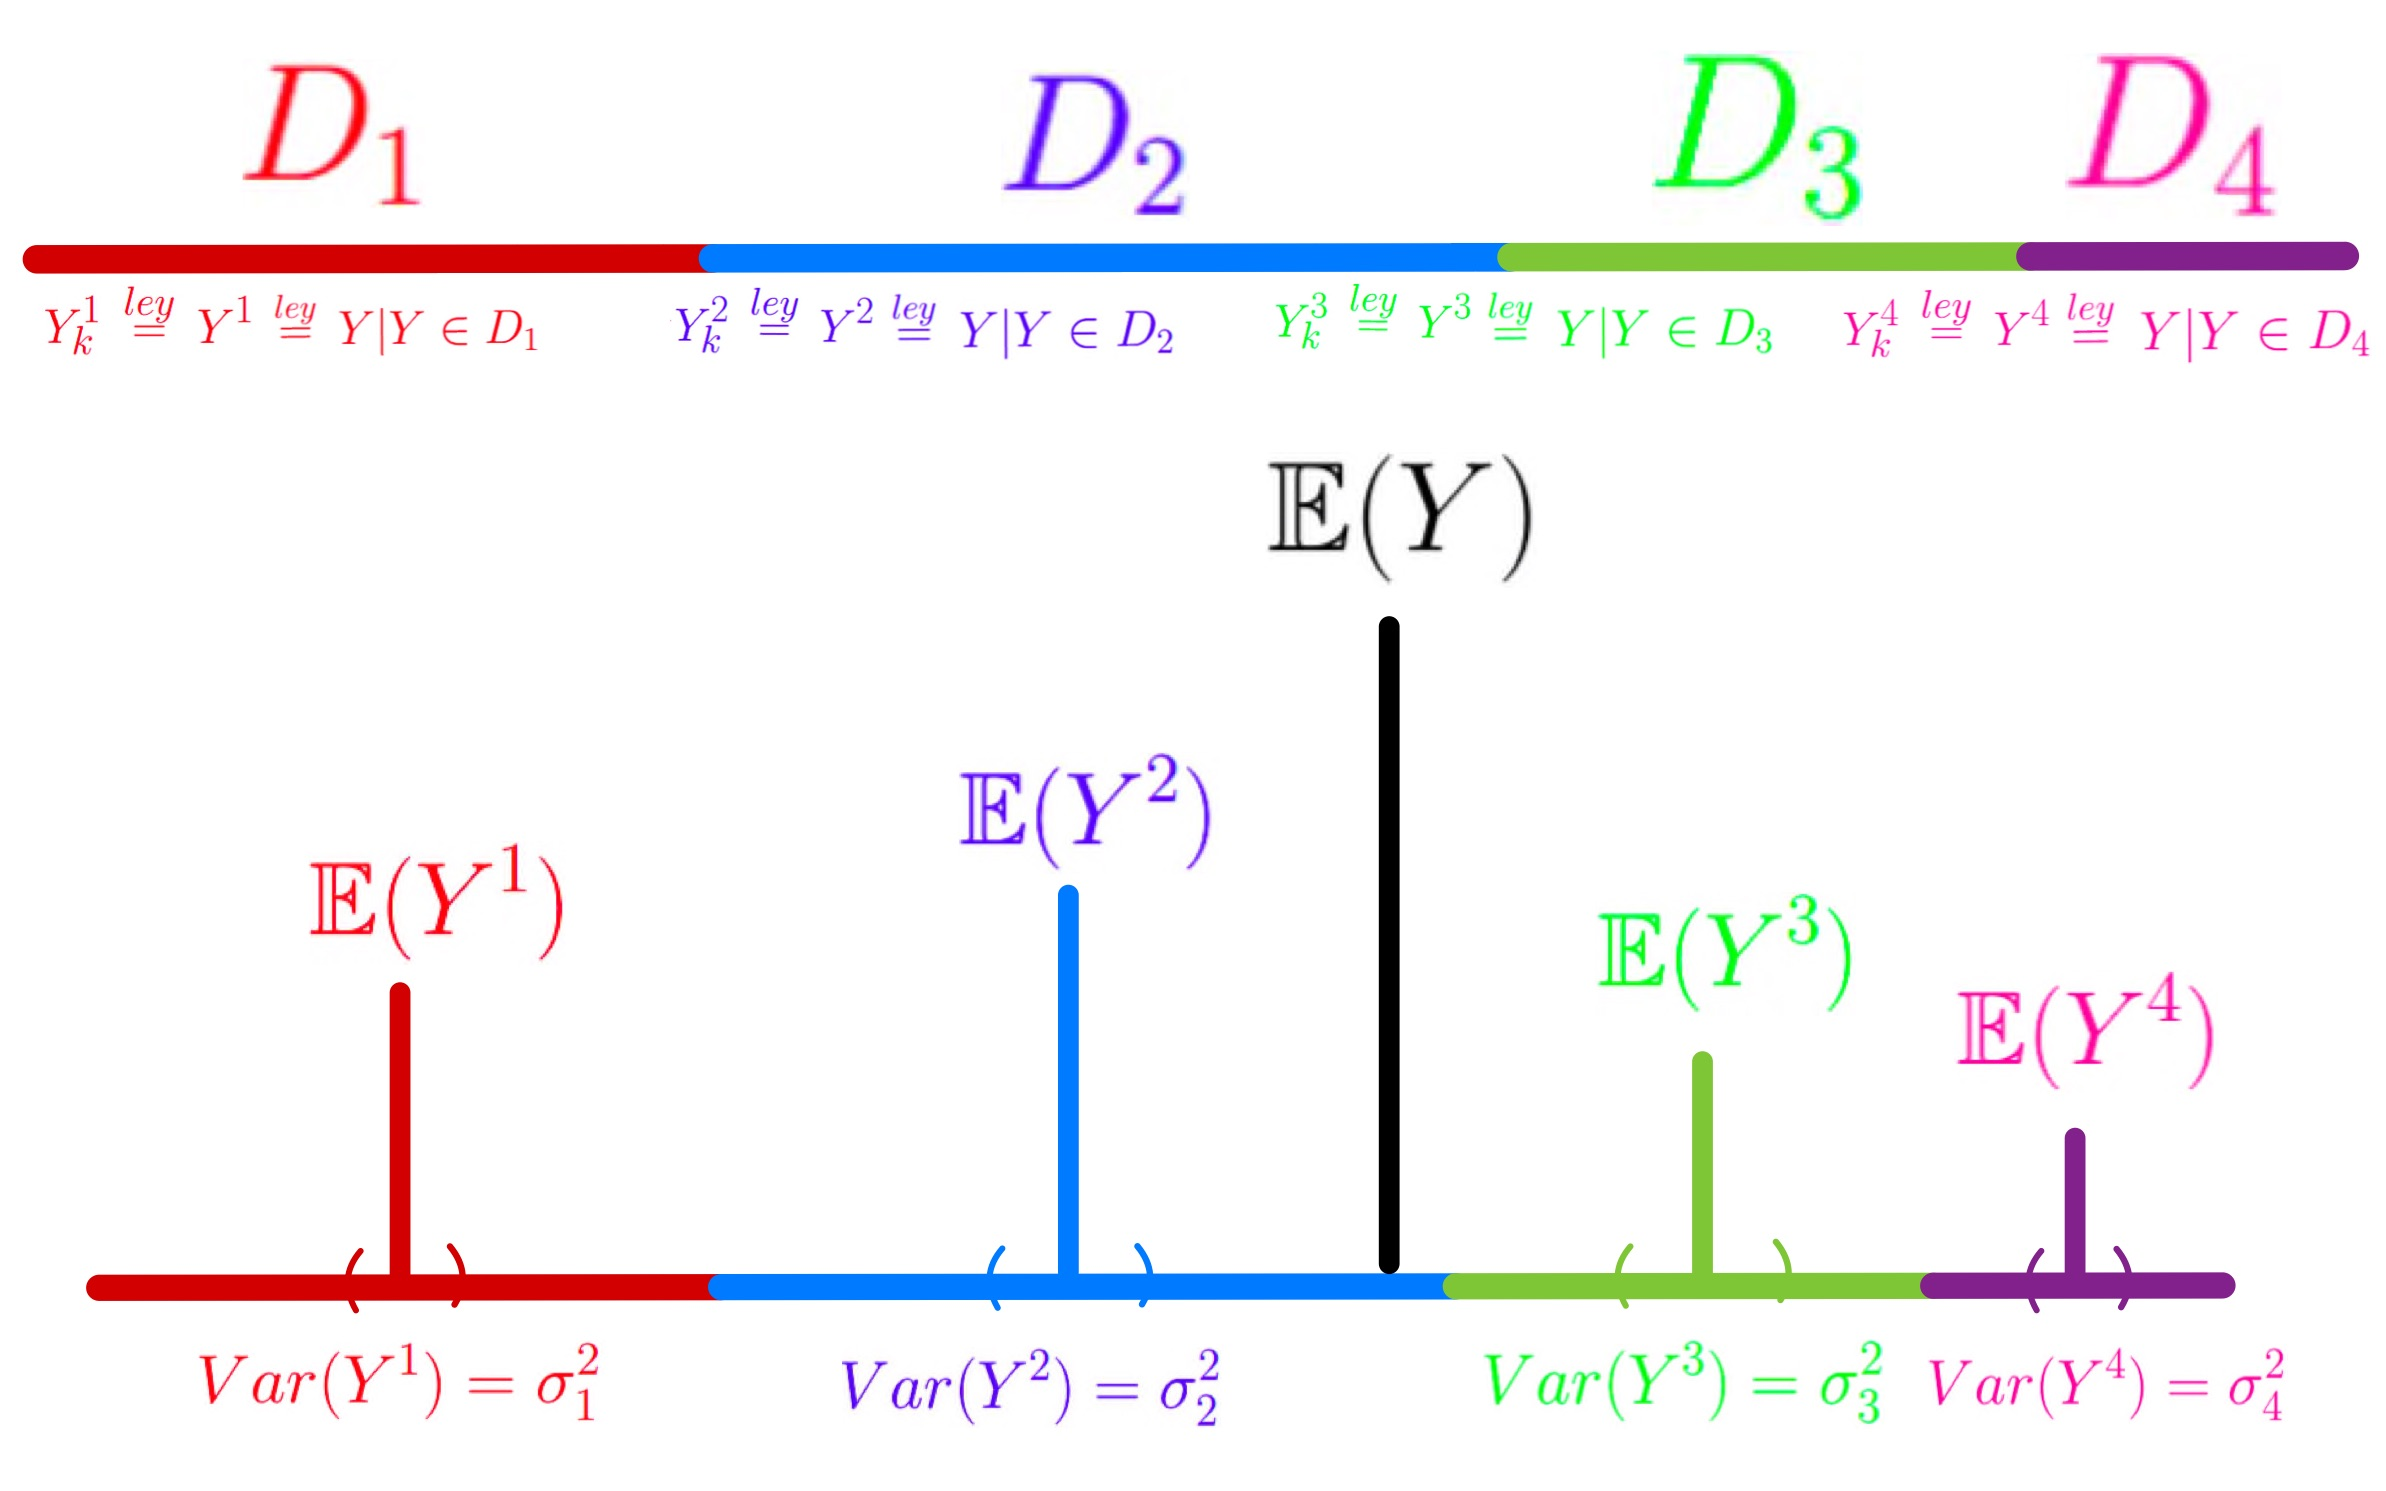
\includegraphics[scale=0.16]{img/clase_09_pag_3.jpg}
    \caption{Ejemplo gráfico de muestreo estratificado}
    \label{fig:estrat}
\end{figure}

\newp Notemos tambi\'en que  $\sum^k_{j=1}p_j\sigma^2_j= \var(\hat{Y}_n)$ si elegimos  $n_j\approx p_jn$.  Vemos entonces que, en este caso,   si $\exists j\tq\E(Y^j)\neq\E(Y)$ tendremos que $\var(\bar{Y}_n)>\var(\hat{Y}_n)$, donde $\hat{Y}$ es el estimador usual.   Dicho de otro modo, basta con que haya algún estrato para el cual la esperanza no sea igual a la esperanza de $Y$, para que se reduzca la varianza con esta elecci\'on de $n_j$'s.


% \newp Se puede escoger $n_1,\dots,n_k$ tal que $n_1+\dots+n_k=n$ de manera aún mejor resolviendo:
\newp Más aún, podemos elegir los $n_j$'s de manera aproximadamente  \'optima,  resolviendo:
\begin{alignat*}{2}
    \displaystyle\min_{n_1,\dots,n_k\geq0}& & \sum^k_{j=1}\sigma^2_j\frac{p_j^2}{n_j}\\
    \mbox{s.a.  }& \mbox{    } & n_1+\dots+n_k=n 
\end{alignat*}
suponiendo los $n_j$ reales y aplicando KKT.  Obtenemos as\'i como soluci\'on entera:
$$ n_j\approx\displaystyle n\bigg(\frac{p_j\sigma_j}{\sum^k_{l=1}p_l\sigma_l}\bigg) \, .$$
Los $\sigma_j$ a su vez, se pueden estimar con simulaciones piloto.

% $$ \color{red} \E(Y^1) \espacio \color{blue} \E(Y^2) \espacio \color{negro} \E(Y)
% \espacio \color{green} \E(Y^3)\espacio  \color{magenta} \E(Y^4)$$
% $$ \color{red} Var(Y^1)=\sigma^2_1 \espacio \color{blue} Var(Y^2)=\sigma^2_2 \espacio \color{green} Var(Y^3)=\sigma^2_3 \espacio  \color{magenta} Var(Y^4)=\sigma^2_4$$
% \big
% $$ \color{red} Y^1_1,\dots,Y^1_{n_1} \espacio \color{blue} Y^2_1,\dots,Y^2_{n_2} $$
% $$ \color{red} \overset{ley}{=}\,Y^1\,\overset{ley}{=}\,Y|Y\in D_1 \espacio \color{blue} \overset{ley}{=}\,Y^2\,\overset{ley}{=}\,Y|Y\in D_2 $$
% $$\color{green} \overset{ley}{=}\,Y^3\,\overset{ley}{=}\,Y|Y\in D_3 \espacio  \color{magenta} \overset{ley}{=}\,Y^4\,\overset{ley}{=}\,Y|Y\in D_4 $$
% $$\color{green} Y^3_1,\dots,Y^3_{n_3} \espacio  \color{magenta} Y^4_1,\dots,Y^4_{n_4} $$


\newpage
\section{Cadenas de Markov (CM)}
Este capítulo contiene definiciones y resultados que ya han sido abordados en el curso Cadenas de Markov. No obstante, nos interesaremos también en simular cadenas de Markov de manera eficiente. También se propondrán algoritmos para simular la distribución invariante de una cadena.

\newp Para revisar el tema con mayor profundidad, se puede consultar  ``Markov Chains'' de J. Norris \cite{norris} o ``Processus de Markov et applications'' de E. Pardoux \cite{pardoux}.
\subsection{Recuerdo}
En esta sección recordaremos las bases de Cadenas de Markov. 
\subsubsection{Definición}
\begin{definition}[Cadena de Markov]
Sea $E$ un conjunto numerable, $P=(P_{xy})_{x,y\in E}$ matriz estocástica y $\lambda=(\lambda_x)_{x\in E}$ vector de probabilidad inicial.

La $(X_n)_{n\in N}$ sucesión de variables aleatorias con $X_n:\edp \to E$ se dice \textbf{Cadena de Markov} C.M.($\lambda,P$) (homog\'enea) si:
\begin{itemize}
    \item $\forall n \in N, \forall x_0,\dots,x_{n+1}\in E \, ,$
    $$ \P(X_{n+1}=x_{n+1}|X_n=x_n,\dots,X_0=x_0) = P_{x_n,x_n+1} \, .$$
    \item $\forall x_0\in E$, $\P(X_0=x_0)=\lambda_0 \, .$
\end{itemize}
\end{definition}

\begin{property}
Algunas consecuencias:
\begin{itemize}
    % \item $\P(X_{n+1}=x_{n+1}|X_n=x_n) = P_{x_nx_{n+1}}$ \, .
    \item $\P(X_{n+1}=y|X_n=x) = P_{xy}$ \, .
    \item $X$ es $CM(\lambda,P)$ si y solo si $$\P(X_0=x_0,\dots,X_n=x_n)=\lambda_{x_0}P_{x_0,x_1}\dots P_{x_{n-1}x_n}\, .$$
\end{itemize}
\end{property}

\subsubsection{Definiciones y propiedades importantes}
\begin{notation}
Denotaremos
\begin{itemize}
    \item $\P_\mu(\cdot)$ a la ley de $\xcm$ cuando $X_0\sim\lambda=\mu$ \, .
    \item $\P_x(\cdot)=\P_{\delta_x}(\cdot)$, con $\delta_x$ masa de Dirac en $x\in E$ \, .
\end{itemize}
\end{notation}

\begin{definition}[$x$ ``pasa'' a $y$]
Sea $X=\xcm$, decimos que $x$ ``pasa'' a $y$ si
$$\P_x(\exists n\geq 0 \tq X_n=y)>0 \, ,$$
y se denota $x\longrightarrow y$.
\end{definition}
\begin{remark}
$x\longleftrightarrow y$ es relación de equivalencia (donde $x\longleftrightarrow y$ si $x\longrightarrow y$ y $y\longrightarrow x$).
\end{remark}
\begin{definition}[Cadena irreducible]
Una cadena $X=\cm$ se dice irreducible si $E$ es la única clase de equivalencia para $\longleftrightarrow$ \, .
\end{definition}
\begin{property}[de Semigrupo]
Sea $X\sim\cm$, entonces $$ \P_X(X_n=y)=(P^n)_{xy} \, .$$
\end{property}
\begin{definition}[Filtración]
Sea $\edp$ un espacio de probabilidad. Sea $(\mathcal{F}_i)_{i\in\N}$ una familia de sub-$\sigma$-álgebras de $\mathcal{F}$. \\ Si $\forall i,j\in\N, i<j$ tenemos $$\mathcal{F}_i\subseteq\mathcal{F}_j \, ,$$
entonces $(\mathcal{F}_i)_{i\in\N}$ se dice una filtración.
\end{definition}
\begin{remark}
Sea $(X_n)_{n\in\N}$ C.M. familia $(\mathcal{F}_i)_{i\in\N}$, dada por $\mathcal{F}_n=\sigma(X_0,\dots,X_n)\, \forall n\in\N$, es una filtración.
\end{remark}
\begin{theorem}[Propiedad de Markov]
Sea $X\sim\cm$ entonces $\forall F:E^\N \to \R$ medible y acotada se tiene
% $$ \E(F(X_{n+1},X_{n+2},\dots)|X_0,\dots,X_n)=\E_{X_n}(F(X_1,X_2,\dots)) \, .$$
$$ \E(F(X_{n+1},X_{n+2},\dots)|\mathcal{F}_0,\dots,\mathcal{F}_n)=\E_{X_n}(F(X_1,X_2,\dots)) \espacio c.s.\, ,$$
donde $\mathcal{F}_n=\sigma(X_0,\dots,X_n)$\,.
\end{theorem}
% \begin{remark}
% La familia $\mathcal{F}_n=\sigma(X_0,\dots,X_n)$ es una filtración (i.e., $\mathcal{F}_n\subset\mathcal{F}_{n+1}\subset\dots\subset\mathcal{F}$)
% \end{remark}
\begin{definition}[Tiempo de parada]
Sea $(\mathcal{F}_i)_{i\in\N}$ una filtración y sea $\tau:\Omega\mapsto\N\cup\{\infty\}$ v.a.. $\tau$ se dice tiempo de parada si
$$\forall m\in\N,\espacio \{\tau\leq m\}\in\mathcal{F}_m \, .$$
\newline A la $\sigma$-álgebra $\mathcal{F}_\tau:=\{A\in\mathcal{F}:A\cap\{\tau\leq m\}\forall m \in \N\}$ se le dice su tribu asociada.
\end{definition}
\begin{theorem}[Propiedad de Markov Fuerte]
Sea $X\sim\cm$, entonces
$$ \E(F(X_{\tau+1},X_{\tau+2},\dots)|\mathcal{F}_\tau)=\E_{X_\tau}(F(X_1,\dots)) \mbox{ c.s. en }\{\tau<\infty\} \, .$$
\end{theorem}
\begin{remark}
El tiempo de retorno a $x\in E$ está dado por $\tau_X=\inf\{n\geq1:X_n=x\}$, y es un tiempo de parada.
\end{remark}
\begin{definition}[Recurrencia y Transiencia]
$x\in E$ se dice recurrente si:
$$ \P_x(\tau_x<\infty)=1 \, .$$
En caso contrario se dice transiente.
\end{definition}
\begin{remark}
Recurrencia es una propiedad de clase.
\end{remark}
\vspace{1cm}\\
\begin{proposition}
\beforeitemize
\begin{itemize}
    \item Una $CM(\lambda,P)$ irreducible se dice recurrente/transiente si $x\in E$ lo es.
    \item Toda $\cm$ irreducible en $E$ finito es recurrente.
\end{itemize}
\end{proposition}
\begin{theorem}
\label{theorem:visitas}
Sea $X\sim\cm$ y denotemos
$$ N_x:=\displaystyle\sum_{n\in\N}\mathbf{1}_{\{X_n=x\}} \, ,$$
que corresponde al \textbf{número de visitas} de la cadena al estado $x\in E$.
\newline Entonces son equivalentes:
\begin{itemize}
    \item $x\in E$ recurrente.
    \item $N_x=\infty \mbox{ }\P_X-{ c.s.}$.
    \item $\displaystyle\sum_{n\in \N}(P^n)_{xx}=\E_x(N_x)=\infty$.
\end{itemize}
\end{theorem}
\begin{definition}[Medida y Probabilidad Invariante]
Sea $X\sim\cm$, $\gamma=(\gamma_x)_{x\in E}$ con $\gamma_x\geq0$ se dice \textbf{medida invariante} (con respecto a $P$) si
$$ \gamma P = \gamma \, ,$$
esto es:
$$ \sum_{x\in E}\gamma_xP_{xy}=\gamma_{y}\mbox{ }\forall y\in E \mbox{ y }\gamma\neq 0 \, .$$
Una \textbf{probabilidad invariante} $\pi$ es una medida invariante finita tal que $\sum_{x\in E}\pi_x = 1$ \,.
\end{definition}
\begin{proposition}
Sea $\pi$ probabilidad invariante, si $X\sim\cm$:
$$ (X_{n+m})_{n\in \N}\sim CM(\pi,P) \mbox{ }\forall n\in \N \, .$$
En particular $Ley(X_n)=\pi \mbox{ }\forall n \in\N$.
\end{proposition}
\begin{theorem}
Sea $X$ $CM$ irreducible y recurrente, entonces existe una única $\gamma$ medida invariante  (salvo constante multiplicativa) tal que $\gamma_y>0\espacio \forall y \in E$.
\newline Más aún para cada $x$, 
$$\gamma_y^{(x)}:=\E_x\left(\displaystyle\sum^{\tau_x}_{n=1}\mathbf{1}_{\{X_n=y\}}\right),\espacio y\in E \, ,$$
es la única medida invariante tal que $\gamma_x^{(x)}=1$.
\end{theorem}
\begin{remark}
Notemos que $\gamma_y^{(x)}$ es el número esperado de visitas a $y$ entre dos visitas consecutivas a $x$\,.
\end{remark}
\begin{definition}[Recurrencia Positiva o Nula]
Denotamos $m_x=\E_x(\tau_x)$ como el tiempo de retorno esperado a $x$\,.
\newline Un estado $x$ se dice recurrente positivo si $m_x<\infty$ y recurrente nulo si $m_x=\infty$.
\end{definition}
\begin{remark}
Recurrencia positiva y nula son propiedades de clase y 
$$\E_x(\tau_x)<\infty\ssi\E_x(\tau_y)<\infty \mbox{ }\forall y\longleftrightarrow x \, .$$
\end{remark}
\begin{theorem}
Sea $X \mbox{ una } CM$ irreducible, las siguientes son equivalentes:
\begin{itemize}
    \item $x\in E$ es recurrente positivo.
    \item Todo $x\in E$ es recurrente positivo.
    \item $\exists ! \pi$ medida invariante para $P$ estrictamente positiva, y está dada por:
    $$ \pi = (\pi_x=m_x^{-1})_{x\in E}>0 \, .$$
\end{itemize}
\end{theorem}
\begin{remark}
$X\sim\cm$ irreducible en $E$ finito $\implies$ $X$ recurrente positiva.
% \newline Por ejemplo si simulamos una fila, tenemos una cantidad no acotada de clientes posibles, por ende nuestro espacio de estados está indexado por los naturales. Sin embargo podemos considerar ciertas cotas. Por ende al simular acotaremos el espacio de estados de modo que $E$ será finito. La irreducibilidad entonces nos garantizará la existencia de una distribución invariante.
\newline En la práctica, para efectos de simulaciones siempre nos restringiremos a espacios finitos.  En los casos en que la cadena es recurrente positiva, esta suposición es suficientemente representativa.
\end{remark}
\begin{notation}
$\P_\mu(X_n=y)=\mu P^n$
\end{notation}
\begin{definition}[Aperiodicidad]
$X$ se dice aperiódica si $\forall x\in E,\exists n_0\in\N\tq$
$$(P^n)_{xx}>0\espacio \forall n\geq n_0 \, .$$
\end{definition}
\begin{theorem}
Sea $X=(X_n)_{n\in \N}$ $CM$ irreducible, entonces:
\begin{itemize}
    \item[(a)] Si $X$ es transiente o recurrente nula, $\forall\mu,\forall y\in E$,     $$ \P_\mu(X_n=y)\conv 0 \, .$$
    \item[(b)] Si $X$ es recurrente positivo, $\forall\mu,\forall y\in E$,
    $$ \displaystyle\frac{1}{n}\sum^n_{k=0}\P_\mu(X_k=y)\conv \pi_y>0 \, ,$$
    con $\pi$ distribución invariante.
    \item[(c)] Si $X$ es recurrente positiva y aperiódica, $\forall\mu,\forall y\in E$,
    $$ \P_\mu(X_n=y)\conv \pi_y \, .$$
\end{itemize}
\end{theorem}

% \\ \vspace{3cm}
\subsection{Simulación de cadenas de Markov}
El siguiente resultado es útil para entender la construcción de cadenas de Markov. En particular será importante para su simulación.
\begin{proposition}
\label{propsimmarkov}
Sean $X_0$ v.a. en $E$, $(Z_n)_{n\in\N}\mbox{ v.a. }\iid$ a valores en un espacio medible $(F,\Sigma)$ independientes de $X_0$. Sea $\Phi:E\times F\to E$ medible, entonces si definimos recursivamente:
$$X_{n+1}:=\Phi(X_n,Z_{n+1}) \espacio \forall n\in\N \, ,$$
luego $\xcm$ es una cadena de Markov $CM(\nu,Q)$ con $\nu=Ley(X_0)$, y $Q_{xy}=\P(\Phi(x,Z_1)=y)$.
\end{proposition}
\begin{proof} \newline
\gris
Por construcción tenemos que $\nu=Ley(X_0)$. \newline Veamos que $(X_n)_{n\in\N}$ es cadena de Markov. Notemos que reemplazando, la probabilidad del cilindro $\P(X_{n+1}=x_{n+1},X_n=x_n,\dots,X_0=x_0)$ puede escribirse como
$$ \P(\Phi(x_n,Z_{n+1})=x_{n+1},\Phi(x_{n-1},Z_n)=x_n,\dots,\Phi(x_0,Z_1)=x_1,X_0=x_0) \, .$$
Pero usando la independencia de los $Z_n$ esto igual a 
$$ \P(\Phi(x_n,Z_{n+1})=x_{n+1})\P(X_n=x_n,\dots,X_0=x_0) \, ,$$
que a su vez por definición corresponde a
$$ Q_{x_nx_{n+1}}\P(X_n=x_n,\dots,X_0=x_0)\, . $$
Por otro lado, sumando sobre todos los estados posibles $x_0,\dots,x_n$ queda que 
$$ \P(X_{n+1}=x_{n+1},X_n=x_n) = \P(\Phi(X_n,Z_{n+1})=x_{n+1})\P(X_n=x_n)=Q_{x_n,x_{n+1}}\P(X_n=x_n) \, .$$
Despejando $Q_{x_nx_{n+1}}$ en ambas ecuaciones se obtiene la propiedad buscada. \findem
\negro
\end{proof}
\vspace{.5cm}\\
A partir de lo anterior deducimos como simular cadenas de markov fácilmente en un computador. En efecto tenemos el siguiente corolario:
\begin{corolary}[Simulación de cadenas de Markov]
Sean $(U_n)_{n\in\N} \iid \sim\unif$, $\lambda=(\lambda_x)_{x\in E}$ vector de probabilidad y $P=(P_{xy})_{x,y\in E}$ matriz estocástica dados, con $E=\{y_0,y_1,\dots,y_n,\dots\}$. % \newline 
Sean 
% $\Phi_0:[0,1]\to E$, $y_n=\Phi_0(u)$ % $u\longmapsto y_n$ 
% si $u\in[\displaystyle\sum^{n-1}_{k=0}\lambda_{y_k},\sum^n_{k=0}\lambda_{y_k}]$  % (que tiene largo $\lambda_{y_n}$)
$$ \Phi_0:[0,1]\to E \, ,\, y_n=\Phi_0(u)\espacio\mbox{si}\espacio u\in[\displaystyle\sum^{n-1}_{k=0}\lambda_{y_k},\sum^n_{k=0}\lambda_{y_k}]$$
y
% \newline $\Phi:E\times[0,1]\to E$, $y_n=\Phi(x,u)$  % $(x,u)\longmapsto y_n$ 
% si $u\in[\displaystyle\sum^{n-1}_{k=0}P_{xy_k},\sum^n_{k=0}P_{xy_k}]$ % (que tiene largo $\P_{xy_n}$).
$$ \Phi:E\times[0,1]\to E\,,\,y_n=\Phi(x,u)\espacio\mbox{si}\espaciou\in[\displaystyle\sum^{n-1}_{k=0}P_{xy_k},\sum^n_{k=0}P_{xy_k}] \, .$$
Entonces el proceso $X_0$ definido por
$$ X_0:=\Phi_0(U_0), \mbox{ }X_{n+1}:=\Phi(X_n,U_{n+1}), n\in\N\, ,$$
es una cadena de Markov de parámetros $\lambda$, $P$.
\end{corolary}
\begin{proof}
\gris
En la Proposición \ref{propsimmarkov} tomar $Z_n=U_n$, $X_0=\Phi_0(U_0)$, y notar que $\P(X_0)=\lambda_y$ y $\P(\Phi(x,Z_1)=y)=P_{xy}.$ \findem
\negro
\end{proof}
% \vspace{.5cm} \\
\begin{remark}
Siempre podemos asumir que $E=\{y_0,\dots,y_n,\dots\} = \{0,1,\dots,n,\dots\}=\N$.
\newline Luego, para simular $X_0\sim\lambda$ y cada transición $Ley(X_{n+1}|X_n=x)=P_{x_0}$, podemos usar simulaciones de variables discretas en $\N$ como las vistas en sección \ref{disc}.
\end{remark}
% \vspace{1.5cm}\\
\subsection{Ley de grandes números para cadenas de Markov}
\begin{theorem}[Ley de grandes números para CM o Teorema ergódico]
\label{lgn_cm}
Sea $X=\xcm$ cadena de markov recurrente positiva e irreducible y $\pi$ su distribución invariante. Entonces $\forall\mu$ distribución inicial, $\forall f:E\to\R$ acotada,
$$ \displaystyle\frac{1}{n}\sum^n_{k=0}f(X_k)\conv\langle\pi,f\rangle=\sum_{y\in E}\pi_y f(y), \mbox{ }\P_\mu-c.s. \, .$$
En particular, $\forall y\in E$:
$$ \displaystyle\frac{1}{n}\sum^n_{k=0}\mathbf{1}_{\{X_k=y\}}\conv\pi_y=\P_\pi(X_0=y) \, \mbox{ }\P_\mu-c.s. \,  .$$
Como consecuencia \textbf{podemos aproximar integrales con respecto a $\pi$ usando una sola trayectoria de $X$.} 
\end{theorem}
\begin{proof}
\gris Seguiremos la demostración de ``Processus de Markov et applications'' % capítulo 3 
de E. Pardoux \cite{pardoux}.

Estudiaremos primero el límite $\displaystyle\frac{N_x(n)}{n}$ cuando $n\to\infty$, donde
$$ N_x(n):=\displaystyle\sum_{1\leq k\leq n}\mathbf{1}_{\{X_k=x\}}$$
es el número esperado de visitas al estado $x$ antes de $n$.

Denotamos $S^0_x,S^1_x,\dots,S^k_x,\dots$ los largos de las sucesivas excursiones $\mathcal{E}_0,\mathcal{E}_1,\dots,\mathcal{E}_k,\dots$ de la cadena recurrente $X$  partiendo y terminando en $x$. Tenemos que
$$ S^0_x+S^1_x+\dots+S^{N_x(n)-1}_x \leq n < S^0_x+S^1_x+\dots+S^{N_x(n)-1}_x+S^{N_x(n)}_x \, ,$$
con lo cual tenemos que
$$ \displaystyle \frac{S^0_x+S^1_x+\dots+S^{N_x(n)-1}_x}{N_x(n)} \leq \frac{n}{N_x(n)} < \frac{S^0_x+S^1_x+\dots+S^{N_x(n)-1}_x+S^{N_x(n)}_x}{N_x(n)} \,. $$
Usando la propiedad de Markov fuerte se demuestra que las excursiones $(\mathcal{E}_k)_{k\in\N}$ son $\iid$ y por ende también lo son las v.a.  $(S_x^k)_{k\in\N}$. Adem\'as, cada $S_x^k$ tiene la misa ley que $T_x$ bajo $\P_x$, donde $T_x = \inf\{n > 0: X_n = x\}$. Deducimos que 
$$ \frac{S^0_x+S^1_x+\dots+S^{N_x(n)-1}_x+S^{N_x(n)}_x}{N_x(n)} \conv \E_x(T_x)=m_x \espacio \P_x-c.s. \, .$$
Por Teorema \ref{theorem:visitas}, $N_x(n)\to + \infty \espacio \P_x-c.s. \,$ cuando $n\to \infty$, y entonces obtenemos
$$ \displaystyle \frac{N_x(n)}{n}\conv \frac{1}{m_x} \espacio \P_x-c.s. \,.$$
Sea ahora $F\subset E$ y denotemos $\bar f = \displaystyle \sum_{x\in E}\pi_x f(x)$. Luego, con $c>0$ una cota para $|f|$, se tiene
\begin{alignat*}{2}
\bigg| \frac{1}{n}\sum^n_{k=1}f(X_k)-\bar f\bigg| & = \bigg|\sum_{x\in E}\bigg( \frac{N_x(n)}{n}-\pi_x \bigg)f(x)\bigg|\\
& \leq c\sum_{x\in F}\bigg|\frac{N_x(n)}{n}-\pi_x\bigg|+c\sum_{x\notin F}\bigg(\frac{N_x(n)}{n}+\pi_x\bigg) \\
& = c\sum_{x\in F}\bigg|\frac{N_x(n)}{n}-\pi_x\bigg|+c\sum_{x\in F}\bigg(\pi_x-\frac{N_x(n)}{n}\bigg)+2c\sum_{x\notin F}\pi_x \\
& \leq 2c\sum_{x\in F}\bigg|\frac{N_x(n)}{n}-\pi_x \bigg|+2c\sum_{x\notin F}\pi_x \, .
\end{alignat*}
En la 3era l\'inea cambiamos $\sum_{x\notin F} \frac{N_x(n)}{n} = 1 - \sum_{x\in F}  \frac{N_x(n)}{n} = \sum_{x\in E}  \pi_x - \sum_{x\in F}  \frac{N_x(n)}{n}  $ . Elegimos ahora $F$ tal que $\displaystyle \sum_{x\notin F}\pi_x\leq\frac{\epsilon}{4c}$ y $N(\omega)$ tal que $\forall n\geq N(\omega)$ 
$$ \sum_{x\in F}\bigg|\frac{N_x(n)}{n}-\pi_x\bigg|\leq\frac{\epsilon}{4c}. $$
Entonces, $\forall n\geq N(\omega)$ tenemos $$ \bigg| \frac{1}{n}\sum^n_{k=1}f(X_k)-\bar f\bigg|\leq\epsilon \, $$
concluyendo  la convergencia. \findem
\negro
% Théorème 2.5.7 Pardoux
\end{proof}
\subsubsection{Estimación de matriz de transición}
\begin{corolary}[Estimación de probabilidades de transición]
Sea $\xcm \cm$ recurrente positiva. $\forall \mu$, $\forall x,y\in E$ tal que $P_{xy}>0$,
$$ \displaystyle\frac{1}{n}\sum^n_{k=0}\mathbf{1}_{\{X_{k+1}=y,X_k=x\}} \mbox{ }\overset{\P_\mu-c.s.}{\substack{\longrightarrow \\n \to \infty}}\mbox{ }\pi_xP_{xy}$$
y además,
$$ \displaystyle \frac{\sum^n_{k=0}\mathbf{1}_{\{X_{k+1}=y,X_k=x\}}}{\sum^n_{k=0}\mathbf{1}_{\{X_{k}=x\}}}\mbox{ }\overset{\P_\mu-c.s.}{\substack{\longrightarrow \\n \to \infty}}\mbox{ }P_{xy}\,.$$
\end{corolary}
\begin{proof}
\ejercicio \gris: \newline $(\hat{X}_n)_{n\in\N}:=(X_n,X_{n+1})_{n\in\N}$ es $CM(\hat{\mu},\hat{P})$ en $\hat{E}:=\{(x,y)\in E\times E:P_{xy}>0\}$ con distribución inicial $\hat{\mu}_{(x,y)}:=\mu_xP_{xy}$ y $\hat{P}_{(z,x|(\omega,y))}:=\begin{cases}
P_{xy}
& \mbox{ si }x=\omega \mbox{ ,}\\
0 & \mbox{ si no.}
\end{cases}$ \newline Además es irreducible y con distribución invariante $\hat{\pi}_{(x,y)}=\pi_xP_{xy}$.
\newline Por la parte anterior, aplicada a $\hat{X}\sim CM(\hat{\mu},\hat{P})$,
$$ \displaystyle\frac{1}{n}\sum^n_{k=0}\mathbf{1}_{\{X_{k+1}=y,X_k=x\}} \mbox{ }\overset{\P_\mu-c.s.}{\substack{\longrightarrow \\n \to \infty}}\mbox{ }\pi_xP_{xy} \, ,$$ y tomar cociente (dividir por la aproximación de $\pi_x$). \negro \findem
\end{proof}
\vspace{1.5cm}\\
\subsection{Distancia de Variación total y coupling }
Nos interesa cuantificar la convergencia de cadenas de Markov y en particular encontrar condiciones para convergencia ``rápida'' (geométrica) al equilibrio. Para ello  estudiaremos una noci\'on apropiada de distancia entre probabilidades en $E$.
\begin{definition}[Distancia de variación total]
\label{def:var_tot}
Dadas $\mu$, $\nu\in\mathcal{E}$, con $E$ numerable, su distancia de variación total es $$\|\mu-\nu\|_1=\sum_{x\in E}|\mu_x-\nu_x| \, .$$
o sea, la distancia en $l^1(E)=L^1(E,\#)$ con $\#$ la medida de conteo.
\newline En general, en un espacio medible $(E,\Sigma)$ cualquiera, la distancia en variación total está dada por:
$$ \|\mu-\nu\|_1=\displaystyle\int_E|\frac{d\mu}{d\lambda}(x)-\frac{d\nu}{d\lambda}|\lambda(dx) \, ,$$
donde $\lambda$ es cualquier medida $\sigma$-finita tal que $\mu,\nu \ll \lambda$ (ejemplo: $\lambda=\mu+\nu$), y se puede verificar que en el caso de $E$ discreto esta noci\'on corresponde con la antes dada. 
\end{definition}
\begin{definition}[Coupling]
Dadas $\mu$, $\nu\in\mathcal{P}(E)$, un coupling (o acoplamiento) entre $\mu$ y $\nu$ es un par de variables aleatorias $X$ e $Y:\edp\to(E,\beta)^2$ definido en algún espacio $\edp$ común tal que $X\sim\mu$, $Y\sim\nu$.
\end{definition}
\begin{remark}
Como el espacio de probabilidad es común, podemos samplear $X$ e $Y$ simultáneamente.
\end{remark}
\begin{lemma}[Desigualdad de Coupling]
\label{lemma:des_coup}
$\forall\mu,\nu\in\mathcal{P}(E)$,
$$ \|\mu-\nu\|_1 = \displaystyle 2\inf_{(X,Y) \mbox{ coupling de }\mu\mbox{ y }\nu}\P(X\neq Y)\, .$$
Además, este ínfimo se alcanza. En particular $\forall (X,Y)$ coupling de $\mu$ y $\nu$ se tiene:
$$ \|\mu-\nu\|\leq 2\P(X\neq Y) \, .$$
A esta última se le llama desigualdad de coupling. 
\end{lemma}
\begin{remark}
\beforeitemize
\begin{itemize}
    \item Elegir $X$ e $Y$ de manera inteligente nos permite tener una buena cota para la distancia de variación total.
    \item Siempre existen coupling. Por ejemplo tomar $X\indep Y$, sin embargo esta no es la mejor cota que podemos encontrar.
\end{itemize}
\end{remark}

\begin{proof}[Demostración del Lema \ref{lemma:des_coup}]  % clase 10 pag 12 %16:16
\gris Sea $(X,Y)$ coupling de $\mu,\nu$, entonces
\begin{alignat*}{2}
    \P(X=Y) & = \displaystyle\sum_{x\in E}\P(X=Y=x)  \\
     & \leq \displaystyle\sum_{x\in E}\min\{\mu_x,\nu_x\} \, .
\end{alignat*}
\begin{alignat*}{2}
    \therefore \P(X\neq Y) & = \geq 1-\displaystyle \sum_{x\in E}\min\{\mu_x,\nu_x\}  \\
     &  = \displaystyle \sum_{x\in E}(\mu_x-\min\{\mu_x,\nu_x\}) \, \\
     & = \displaystyle\sum_{x\in E}(\mu_x-\nu_x)_+.
\end{alignat*}
% $\therefore \P(X\neq Y)\geq 1-\displaystyle \sum_{x\in E}\min\{\mu_x,\nu_x\} = $
Luego, como $|x| = |x|_++|-x|_+$\,,
$$ \|\mu_x-\nu_x\|_1 = \displaystyle\sum_{x\in E}|\mu_x-\nu_x|\leq 2\P(X\neq Y) \, .$$
Ahora construiremos explícitamente un coupling ``óptimo'' donde el ínfimo se alcanza. \\ Sea $\alpha = \displaystyle\sum_{x\in E}\min\{\mu_x,\nu_x\}\leq 1$ y $\xi\in\mathcal{P}(E)$ dada por
$$ \xi_x = \alpha^{-1}\min\{\mu_x,\nu_x\}\, .$$
Sean $\xi$, $U$, $V$, $W$ v.a. independientes con leyes $\xi\sim Ber(\alpha)$, $U\sim\xi$, $V\sim\bigg(\bar{\mu}_x\displaystyle:=\frac{(\mu_x-\nu_x)_+}{1-\alpha}\bigg)_{x\in E}$, $W\sim\bigg(\bar{\nu}_x\displaystyle:=\frac{(\nu_x-\mu_x)_+}{1-\alpha}\bigg)_{x\in E}$. Entonces definimos
$$ X:=\begin{cases}
U & \mbox{ si }\xi=1\\
V & \mbox{ si }\xi=0
\end{cases}, \espacio Y:=\begin{cases}
U & \mbox{ si }\xi=1\\
W & \mbox{ si }\xi=0
\end{cases}$$
Veamos que $(X,Y)$ es un coupling de $\mu$ y $\nu$. En efecto
\begin{alignat*}{2}
    \P(X=x) & = \P(X=x|\xi=0)\P(\xi=1)+\P(X=x|\xi=0)\P(\xi=0) \\
     & = \alpha\P(U=x)+(1-\alpha)\P(V=x) \\
     & = \displaystyle \alpha\bigg(\frac{\min\{\mu_x,\nu_x\}}{\alpha}\bigg)+(1-\alpha)\frac{(\mu_x-\nu_x)_+}{1-\alpha} \\
     & = \min\{\mu_x,\nu_x\}+(\mu_x-\nu_x)_+ = \mu_x \, .
\end{alignat*}
Por ende tenemos que $X\sim\mu$. De manera completamente análoga podemos concluir que $Y\sim\nu$.
Veamos ahora que el coupling es óptimo. Notemos que $\P(X\neq Y)=1-\alpha$. En efecto,
\begin{alignat*}{2}
    \P(X\neq Y) & = \P(X\neq Y|\xi=0)\P(\xi=0)+\P(X\neq Y|\xi=1)\P(\xi=1) \\
     & = (1-\P(V=W))(1-\alpha) \\
     & = \bigg(1-\displaystyle\sum_{x\in E}\frac{(\mu_x-\nu_x)_+(\nu_x-\mu_x)_+}{(1-\alpha)^2}\bigg)(1-\alpha) \\
     & = 1-\alpha \, ,
\end{alignat*}
pues $(\mu_x-\nu_x)_+(\nu_x-\mu_x)_+ = 0$. Usando esto tenemos que
\begin{alignat*}{2}
    \|\mu-\nu\|_1 & = \displaystyle \sum_{x\in E}|\mu_x-\nu_x| \\
     & = \displaystyle \sum_{x\in E}[\mu_x+\nu_x-2\min\{\mu_x,\nu_x\}] \\
     & = \displaystyle 2-2\sum_{x\in E}\min\{\mu_x,\nu_x\} \\
     & = 2-2\alpha = 2\P(X\neq Y) \, .
\end{alignat*}
$\therefore$ este coupling alcanza el ínfimo. \findem
\negro 
\end{proof}

\begin{remark}
La distancia en variación total se puede definir en $(E,\Sigma)$ espacio medible cualquiera como
$$ \|\mu-\nu\|_1 = \displaystyle \int_E|\frac{d\mu}{d\lambda}(x)-\frac{d\nu}{d\lambda}(x)|\lambda(dx)\, ,$$
donde $\lambda$ es cualquier medida $\sigma$-finita tal que $\mu,\nu<<\lambda$ (por ejemplo $\lambda=\mu+\nu$).
\\ Esta definición coincide con la del curso de Teoría de la Medida:
$$ \|\mu-\nu\|=|\mu-\nu|(E) \, $$
donde $|\espacio|$ es la medida de variación total; y también con la definición \ref{def:var_tot} que hicimos para el caso $E$ numerable, excepto que esta vale para $E$ espacio medible cualquiera.
\end{remark}
\begin{proposition}%pag 4 c
Sea $E$ numerable, se tiene:
$$ \mu^n\convdebil\mu \espacio \Longleftrightarrow \espacio \|\mu^n-\mu\|_1\conv0\,.$$
\end{proposition}
\begin{proof}
\ejercicio \espacio \gris Indicación: Notar que $E$ es un espacio métrico con $d(x,y)=\mathbf{1}_{x\neq y}$, y toda función es Lipschitz.  La distancia en variación total es un caso particular de una familia de m\'etricas generales definidas sobre medidas de probabilidad, conocidas como distancia de transporte: 
\negro
\end{proof}
\begin{proposition}[Distancia Wasserstein]  %pag 4 d
Sea $(E,d)$ espacio métrico cualquiera, $d$ induce una distancia $W_d$ en $\mathcal{P}(E)$ mediante:
$$ W_d(\mu,\nu) = \displaystyle \inf_{(X,Y)\text{ coupling de }\mu,\nu}\E(d(X,Y)) \, .$$
Se le llama \textbf{distancia de Wasserstein o de transporte}.
\end{proposition}

\subsection{Convergencia Geométrica}
\begin{definition}[Condición de Doeblin]
Decimos que se cumple la condición de Doeblin, denotada por $(D)$, si $\exists n_0\geq1$, $\exists\beta>0$, $\exists m\in\mathcal{P}(E)$ tal que
$$(P^{n_0})_{xy}\geq\beta m_y \mbox{ }\forall x,y\in E \, .$$
\end{definition}
\vspace{.5cm} \\
\begin{remark}
\beforeitemize
\begin{itemize}
    \item  Si vemos $(P^{n_0})_{xy},y\in E$ como medida de probabilidad, $(D)$ dice que esta está minorada por una medida de probabilidad $m_y$ que no depende de $x$.
    \item Cuando se simula una cadena de Markov, si queremos simular una transición entre $x$ e $y$, la condición nos dice que a veces podremos hacerlo sampleando una variable aleatoria con ley $m_y$, olvidándonos de que $x$ partimos. Esta capacidad de ``olvidar el pasado'' nos va a dar la convergencia al equilibrio.
\end{itemize}
\end{remark}

\begin{property}
Consideremos la condición de Doeblin $(D)$, entonces:
\begin{alignat*}{2}
    (D) & \Longleftrightarrow (\exists y\in E)(\exists n_0 \geq 1) \mbox{ tal que }\displaystyle \inf_{x\in E}(P^{n_0})_{xy}>0 \\
     & \Longleftrightarrow (\exists n_0 \geq 1) \mbox{ tal que } \displaystyle \sum_{y\in E}\inf_{x\in E}(P^{n_0})_{xy}>0 \, .
\end{alignat*}
\end{property}
\begin{proof}
\ejercicio
\end{proof}
\begin{remark}
\beforeitemize
\begin{itemize}
    \item $\beta\in[0,1]$ \, (sumando con respecto a $y$ en $(D)$) y $\beta<1$ a menos que $(P^{n_0})_{xy}=m_y$ $\forall x,y\in E$ .
    \item $(D)$ es raramente satisfecha cuando $|E|=+\infty$ \, .
    Típicamente sucederá que $\forall n\in \N$, $\forall y\in E$ $\inf_{x\in E}(P^n)_{xy}=0$ \, .
    \item $P$ irreducible y aperiódica y $|E|<\infty$ implica que $(D)$ se cumple.
    \newline     \ejercicio
\end{itemize}
\end{remark}
\begin{theorem}
Supongamos $P$ irreducible y que cumple $(D)$. Entonces $P$ es aperiódica y recurrente positiva, y si $\pi$ denota su distribución invariante, se tiene
$$ \|\mu^{P^n}-\pi\|_1\leq 2(1-\beta)^{\lfloor\frac{n}{n_0}\rfloor}, \mbox{ } \forall \mu\in \mathcal{P}(E),\forall n\in\N\,,$$
donde $\beta\in(0,1)$ y $n_0\geq 1$ vienen de $(D)$. Es decir, la convergencia  al equilibrio tiene lugar a tasa geométrica.
\end{theorem}
\begin{proof} % Clase 11 10:50 pag 6-10
\gris
\beforeitemize
\begin{enumerate}
    \item Probemos que $\forall\mu,\nu\in\mathcal{P}(E),\,\forall n\in\N$
    $$ \|\mu P^n-\pi\|_1\leq 2(1-\beta)^{\lfloor\frac{n}{n_0}\rfloor} \, .$$
    Basta construir para cada $n$ un coupling $(X_n,Y_n)$ de $\mu P^n$ y $\nu P^n$ tal que
    $$ \P(X_n\neq Y_n)\leq(1-\beta)^{\lfloor\frac{n}{n_0}\rfloor} \, $$
    y tomar despu\'es $\nu=\pi$, de modo que $\nu P^n=\pi$ para todo $n$.  
    Escribimos: $n=k n_0+j$, con $j<n_0$.
    \begin{itemize}
        \item Notar que $Q_{xy}:=\displaystyle\frac{(P^{n_0})_{xy}-\beta_{m_y}}{1-\beta}$ es matriz estocástica por $(D)$.
        \\ Sea $f:E\times[0,1]\mapsto E$ función de transición asociada:
        $$ \P(f(x,U)=y)=Q_{xy}\text{ si }U\sim\unif\,.$$
        \item Sean $X_0\sim\mu$, $Y_0\sim \nu$, $\xi_l\sim Ber(\beta)$, $U_l\sim\unif$, $W_l\sim m, \, l=1,\dots,k$ independientes. Definimos recursivamente para $l=0,\dots,k-1$
        $$X_{(l+1)n_0} = \begin{cases}
                W_{l+1} & \mbox{ si }\xi_{l+1}=1\\
                f(X_{l_{n_0}},U_{l+1}) & \mbox{ si no}
            \end{cases}$$
        $$Y_{(l+1)n_0} = \begin{cases}
                W_{l+1} & \mbox{ si }\xi_{l+1}=1\\
                f(Y_{l_{n_0}},U_{l+1}) & \mbox{ si no} \, .
            \end{cases}$$
        Se puede probar que
        $$ (P^{n_0})_{xy} = \begin{cases}
                \P(X_{(l+1)_{n_0}}=y|X_{l_{n_0}}=x) \\
                \P(Y_{(l+1)_{n_0}}=y|Y_{l_{n_0}}=x)
            \end{cases} $$
        y $$ (X_{l_{n_0}})^k_{l=0}\sim C.M.(\mu,P^{n_0})$$
        $$ (Y_{l_{n_0}})^k_{l=0}\sim C.M.(\nu,P^{n_0})\,$$
        pues ambas son construcciones recursivas con ``innovaciones'' independientes.
        \item Sea ahora $\hat{f}:E\times[0,1]\mapsto E$ función de transición asociada a $P^j$ y $\hat{U}\sim\unif$, independiente a todo lo anterior. Entonces $(X_n,Y_n)$ con
        $$ X_n := \hat{f}(X_{k_{n_0}},\hat{U})$$
        $$ Y_n := \hat{f}(Y_{k_{n_0}},\hat{U})$$
        es un coupling de $\mu P^n$ y $\nu P^n$, 
        y se tiene: $\{X_n\neq Y_n\}\subseteq \displaystyle \bigcap^k_{l=0}\{X_{l_{n_0}}\neq Y_{l_{n_0}}\}\subseteq \bigcap^k_{l=0}\{\xi_l=0\}$,
        $$ \therefore \P(X_n\neq Y_n)\leq (1-\beta)^k=(1-\beta)^{\lfloor\frac{n}{n_0}\rfloor}$$
        $$ \text{ y } \|\mu P^n-\nu P^n\|_1\leq 2(1-\beta)^{\lfloor\frac{n}{n_0}\rfloor} \, ,$$
        gracias al Lema \ref{lemma:des_coup},
        que es lo que queríamos.
    \end{itemize}
    \item Veamos que $\mu P^n$ converge a algo en % $\mathcal{P}(E)$
    $l^1(E)$ (variación total)
    \\ Tomando $\nu = \mu P^m$, $m\in\N$ fijo, obtenemos
    % $$ \longrightarrow \|\mu P^n-\mu P^{n+m}\|_1\leq 2(1-\beta)^{\frac{n}{n_0}+1}\, \forall m\in\N$$
    \begin{alignat*}{2}
        &  \|\mu P^n-\mu P^{n+m}\|_1\leq 2(1-\beta)^{\frac{n}{n_0}+1}\, \forall m\in\N \\
        & \Longrightarrow \{\mu P^n\}_{n\in\N}\text{ suc. de Cauchy en }l^1(E) \\
        & \Longrightarrow \exists \pi\in\mathcal{P}(E) \text{ tal que }\mu P^n\conv\pi\, .
    \end{alignat*}
    \item Notar que $\|\mu P-\nu P\|_1\leq \|\mu-\nu\|_1$, o sea $\nu\mapsto\nu P$ es Lipschitz con respecto a $\|\,\|_1$, por lo que tomando $\nu=\mu P$ tenemos
    $$ \|\mu P^n-\mu P^{n+1}\|_1=\|\mu P^n-(\mu P^n)P\|_1\conv \|\pi-\pi P\|_1 \, .$$
    Por otro lado, como $\mu P^n$ es sucesión de Cauchy, $\|\mu P^n-(\mu P^n)P\|_1\conv=0$, con lo cual $\|\pi-\pi P\|_1=0$. Sigue que $\pi$ es medida de probabilidad invariante y $P$ es recurrente positiva.
    \\ Además, $(P^n)_{xx}\conv\pi_x>0$, luego $P$ es aperiódica. Finalmente tomando $\nu=\pi$
    $$ \Longrightarrow \|\mu P^n-\pi\|_1\leq 2(1-\beta)^{\lfloor\frac{n}{n_0}\rfloor}\, \forall n\in\N\, .$$
    $\findem$
\end{enumerate}
\negro
\end{proof}
\subsection{Teorema central del límite para CM}
\begin{definition}[Uniforme ergodicidad]
Una % cadena de Markov 
$\cm$ (o su matriz de transición) se dice uniformemente ergódica si es irreducible, recurrente positiva y $\exists m>0$, $\rho\in(0,1)$ tal que $\displaystyle\sum_{y\in\E}|(P^n)_{xy}-\pi_y|\leq M\rho^n$, $\forall n\in\N$, $\forall x\in E$\,.
\end{definition}
\begin{theorem}[T.C.L para cadenas de Markov]
\label{tcl_markov}
Sea $(X_n)_{n\in \N}$ irreducible, aperiódica y uniformemente ergódica. Sea $\pi$ su ley invariante y $f\in L^2(E,\pi)$, es decir,  $\displaystyle\sum_{x\in E}f^2(x)\pi_x<\infty$. Entonces
$$ \displaystyle \sqrt{n}\bigg(\frac{\sum^n_{k=0}f(X_k)-\langle\pi,f\rangle)}{n}\bigg)\convley\normal(0,\sigma^2_f)\,,$$
con $\sigma^2_f=\langle\pi,(Qf)^2\rangle-\langle\pi,(PQf)^2\rangle$ donde $(Qf)_x=\displaystyle\sum^\infty_{n=0}\E_x(f(X_n))$, $x\in E$.
\newline Notar que $\displaystyle\sum^\infty_{n=0}$ converge gracias a la uniforme ergodicidad.
\end{theorem}
\begin{proof}
\gris En Pardoux \cite{pardoux}.
\negro
\end{proof}
\begin{corolary}
Sea $\xcm$ una cadena de Markov irreducible que satisface $(D)$, en particular si $E$ es finito, satisface el TCL (\ref{tcl_markov}).
\end{corolary}
\subsection{Simulación exacta de una ley invariante}
Consideremos $(X_n)_{n\in \N}\sim \cm$ irreducible, recurrente positiva y aperiódica. Sabemos que:
$$ X_n\convley X_\infty\sim\pi$$
Sin embargo esto sigue siendo una aproximación. Sin embargo nos gustaría simular una $X_\infty$ que distribuya $\pi$ de manera \textbf{exacta}, no aproximada. Se darán dos condiciones y algoritmos para aquello.
\subsubsection{Algoritmo simulación perfecta}
Supongamos $(D)$ con $n_0=1$ y sea $\beta=\displaystyle\sum_{y\in E}\inf_{x\in E}P_{xy}\in(0,1)$ y consideremos la siguiente elección de $m$:
\begin{itemize}
    \item $m\in\mathcal{P}(E)$, con $m_y:=\displaystyle\frac{\inf_{x\in E}P_{xy}}{\beta}$, $y\in E$\,.
    \item $\bigg(Q_{xy}=\displaystyle\frac{P_{xy}-\beta m_y}{1-\beta}\bigg)_{x,y\in E}$ \, matriz estocástica.
\end{itemize}
Notemos que si simulamos $\xi\sim Ber(\beta)$, $Z\sim m$, $Y\sim Q_{X_0}$ independientes, entonces $X$ dada por 
$$ X:=\begin{cases}
Z
& \mbox{ si }\xi=1\\
Y & \mbox{ si }\xi=0
\end{cases}\espacio $$
 tiene ley $P_{x_0}$. En efecto:
\begin{alignat*}{2}
    \P(X=z) & = \P(X=z|\xi=1)\P(\xi=1)+\P(X=z|\xi=0)\P(\xi=0) \\
     & = \P(Z=z)\beta + \P(Y=z)(1-\beta)\\
     & = \beta m_Z+(1-\beta)Q_{xz} = P_{xz}\,,
\end{alignat*}
i.e., obtenemos $P_{xz}$ por construcción.
\newp Entonces construimos una función de transición $f:E\times [0,1]\to E$ tal que si $U\sim\unif$,
$$ \P(f(x,U)=y|U\leq \beta)=m_y$$
$$ \P(f(x,U)=y|U>\beta)=Q_{xy}\,.$$
Basta tomar:
\begin{itemize}
    \item $f_1:E\times[0,1]\to E$ función de transición asociada a $Q:\P(f_1(x,U)=y)=Q_{xy}$\,.
    \item $f_0:[0,1]\to E$ función para simular $m:\P(f_0(U)=y)=m_y$\,.
\end{itemize}
Y definimos: 
$$f(x,u)=f_0\bigg(\frac{u}{\beta}\bigg)\mathbf{1}_{u\leq\beta}+f_1\bigg(x,\frac{u-\beta}{1-\beta}\bigg)\mathbf{1}_{u>\beta}\, .$$
Esta función cumple lo requerido (\ejercicio) y además 
$$\forall x\in E,\espacio \P(f(x,U)=y)=P_{xy}\,.$$
% \vspace{1.5cm}\\
\begin{theorem}[Algoritmo de simulación perfecta]
\beforeitemize
\begin{enumerate}
    \item[(i)] Sean $U_0,U_{-1},U_{-2},\dots,\iid\sim\unif$ y $\tau=\max\{k\leq 0:U_k<\beta\}$\,.
    \item[(ii)] Sea $X_\tau:=f(\bar{x},U_\tau)$ con $\bar{x}$ fijo cualquiera.
    \item[(iii)] Para $k=\tau+1,\tau+2,\dots,-1,0$ sean $X_k=f(X_{k-1},U_k)$ donde las $U_k$ son las mismas uniformes de antes.  % , de modo que $X_k$ tiene ley $Q$\,.
\end{enumerate}
Entonces $-(\tau-1)\sim Geo(\beta)$, $X_\tau\sim m$, $X_\tau\indep-(\tau-1)$ y  % (donde se sampleo es independiente de cuando se hizo), y
$$ X_0\sim\pi\,,$$
donde $\pi$ es invariante para $P$\,.
\end{theorem}
\begin{proof} % clase 11 pag 16
\gris
Sean $k\in\N$, $x_0,x_1,\dots,x_k\in E$,
\begin{alignat*}{2}
    & \P(\tau = -k,X_{-k}=x_k,X_{-(k-1)}=x_{k-1},\dots,X_{-1}=x_{-1},X_0=x_0) \\ & = \P[f(\bar{x},U_{-k})=x_k,U_{-k}<\beta,f(x_k,U_{-(k-1)})=x_{k-1},U_{-(k-1)}\geq\beta,\dots,f(x_{1},U_0)=x_0,U_0\geq\beta] \\
    & = m_{x_k}\beta\cdot Q_{x_k x_{k-1}}(1-\beta)\dots Q_{x_1 x_0}(1-\beta) \, ,
\end{alignat*}
donde usamos que las uniformes son independientes.
Por otro lado, sumando, para $x_0,\dots,x_k$ se verifica que
$$ \P(-(\tau+1)=j,X\tau=x)=m_x\beta(1-\beta)^{j-1} \, ,$$
que es la ley geométrica buscada. Veamos ahora que $\P(X_0=x)$ es invariante.
% $$ \P(\tau=-k,X_{-k}=x_k) = m_{x_k}\beta(1-\beta)^k \, ,$$
% lo cual equivale a que
% $$ \P(\tau+1=-(k-1),X_\tau=x_k) = m_{x_k}\beta(1-\beta)^k \,$$
% con lo cual, colocado en términos de $-(\tau-1)$ y $j$ queda
% $$ \P(-(\tau-1)=j,X_\tau=x)=m_x\beta(1-\beta)^{j-1} \, .$$
\\ Denotando $\mu_x=\P(X_0=x)$, tenemos entonces que 
\begin{alignat*}{2}
    \mu_x & = \displaystyle \sum^\infty_{k=0}\sum_{x_1,\dots,x_k\in E}\P(\tau=-k,X_{-k}=x_k,\dots,X_{-1}=x_1,X_0=x) \\
    & = \sum_{k=0}^\infty(mQ^k)_x\beta(1-\beta)^k \\
    & = \beta\sum^\infty_{k=0}(mQ^{k+1})_x(1-\beta)^{k+1}+\beta m_x \\
    & = \sum_{y\in E}\beta\sum^\infty_{k=0}(mQ^{k})_y(1-\beta)^{k}[(1-\beta)Q_{yx}+\beta m_x] \\
    & = \sum_{y\in E}\P(x_0=y)P_{yx} = \sum_{y\in E}\mu_y P_{yx}\,,
\end{alignat*}
gracias a que $P_{xy}=(1-\beta)Q_{yx}+\beta m_x$\, y que $\P(x_0=y)=\beta\sum^\infty_{k=0}(mQ^{k})_y(1-\beta)^{k}$. \\ Como
$ \mu_x = \displaystyle\sum \mu_yP_{yx}$
tenemos que $\mu_x$ es medida invariante. Como la medida invariante es única concluimos que $\mu_x=\pi\, .$ \findem
\negro
\end{proof}

\subsubsection{Coupling from the past}
Sea $P$ finita irreducible (y entonces recurrente positiva) en un espacio $E=\{1,\dots,N\}$. \\ Sea $f:E\times[0,1]\mapsto E$ la función de transición asociada. Sean $(U_n:n\in\mathbb{Z},y\in E)\sim\unif\iid$ que simulamos una sola vez.
Entonces, tenemos funciones aleatorias independientes
\begin{alignat*}{2}
\Phi_n^y:E & \longmapsto E \\
x & \longmapsto \Phi_n(x) = f(x,U_n)\, ,
\end{alignat*}
con $n\in\mathbb{Z}, y\in E$. Las usaremos para construir, para cada $n\in\N$, $N$ cadenas de Markov $(X_{n,m}^y)_{m\geq n}$, $y=1,\dots,N$, partiendo en tiempo $n$ de los $N$ estados distintos, pero \textbf{coalescentes}. Esto es:
\begin{itemize}
    \item Para cada $y=1,\dots,N$, $X^y_{n,m}$ parte de $y$ y evoluciona usando el flujo $\Phi_m\circ\dots\circ\Phi_n:E\longmapsto E,$ es decir $X^y_{n,m}=\Phi_m\circ\dots\Phi_n(y)$.
    % Sean $(X^1_{n,n},X^2_{n,n},\dots,X^N_{n,n})=(1,2,\dots,N)$ y para $m>n$:
    % donde $x_y=\min\{x\in\{1,\dots,y-1\}:X^y_{n,n-1}=X^x_{n,m-1}\}$.
    \item Si $\exists m>n$ tal que $X^y_{n,m}=X^z_{n,m}=x$, en ese momento coalescen, pues ambas evolucionan desde ahí como $\Phi_{m+k}\circ\dots\circ\Phi_m(x)$, i.e., siguen igual desde aquel punto.
    \item Para cada $n\in-\N$, sea $S_n:=\inf\{m>n:X^1_{n,m}=\dots X^N_{n,m}\}$ el primer instante en que coalescen todas las cadenas iniciadas a tiempo $n$. Notar que $S_n$ puede ser infinito, pues puede ser que en ningún momento se junten todas. En la figura \ref{fig:past} visualizamos como van coalesciendo las cadenas.
    \item Sea $\tau_0:=\sup\{n\leq 0:S_n\leq 0\}$ el último $n\leq 0$ tal que las cadenas iniciadas en $n$ coalescen antes de $m=0$. $\tau_0$ representa aquel tiempo ``menos en el pasado'' tal que al lanzar las cadenas en ese momento hayan coalescido en $0$.
    \item En general, se necesitan condiciones para asegurar que $\tau_0>-\infty$.  % , de existir un orden en $E$, que se refleja en la funciones de transición de alguna forma, entonces si se puede.
\end{itemize}

\begin{figure}
    \centering
    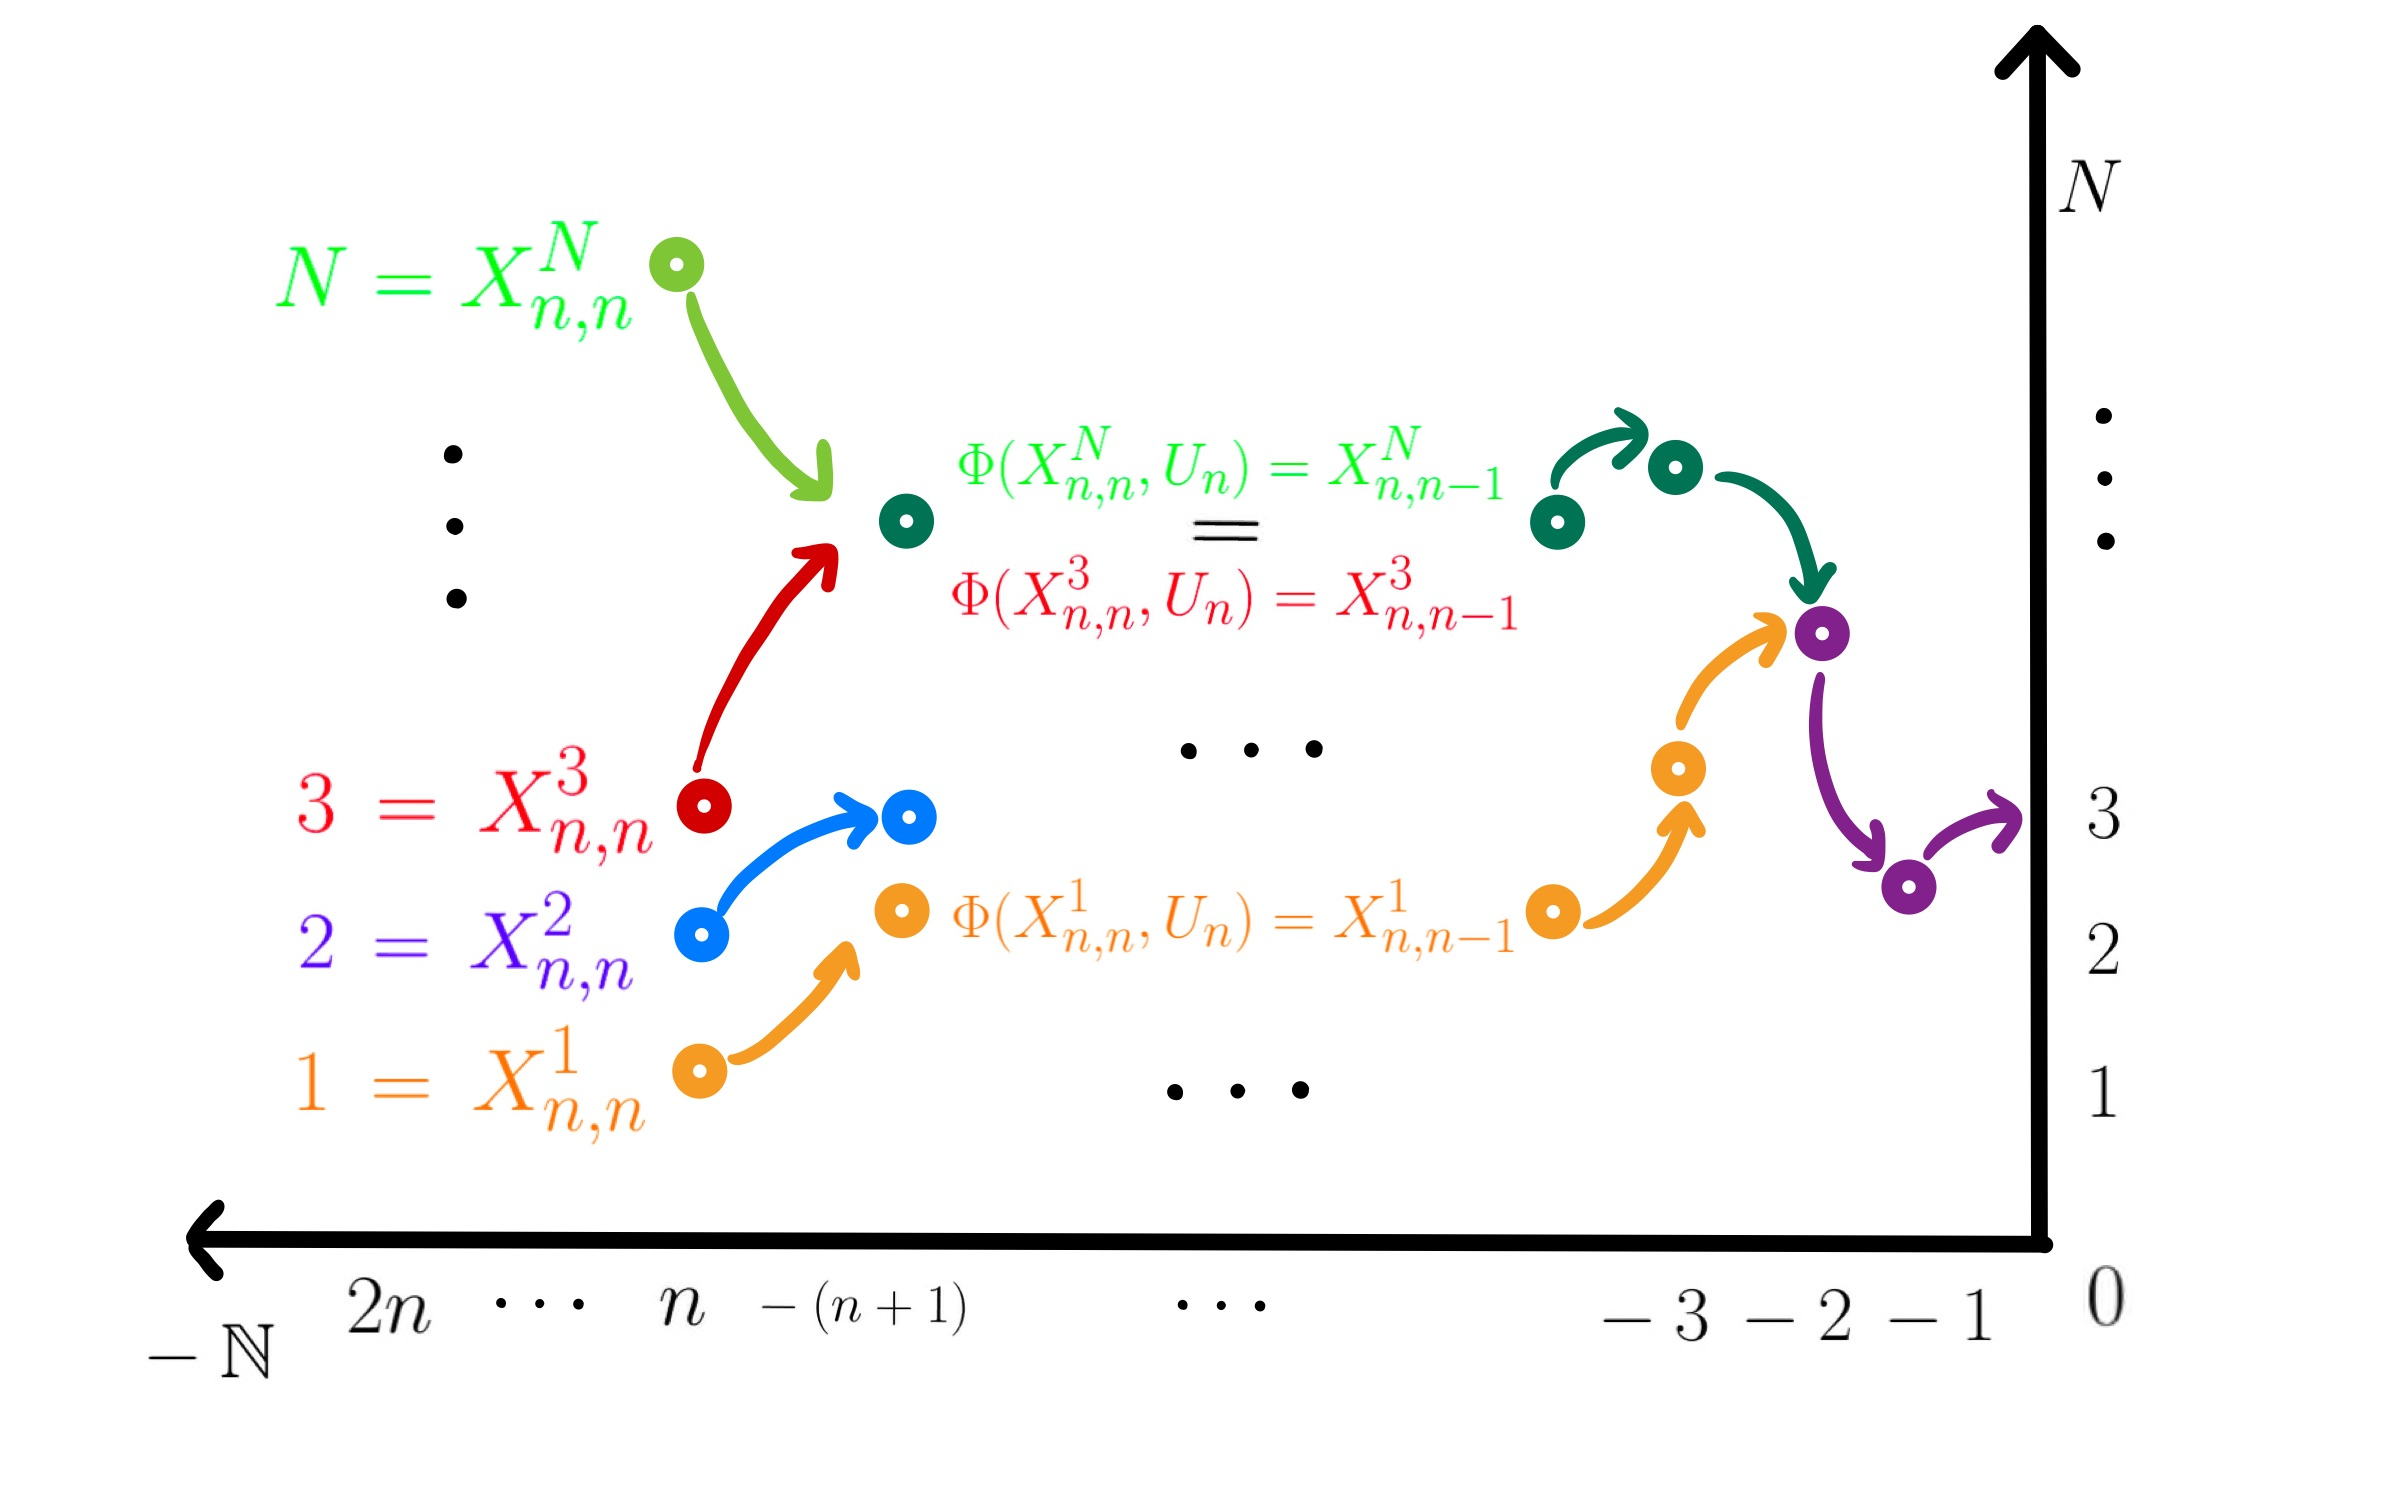
\includegraphics[scale=0.16]{img/clase_12_pag_9.jpg}
    \caption{Ejemplo de $(X^y_{n,m})_{m\geq n}$ que coalescen.}
    \label{fig:past}
\end{figure}

% \Huge
% $$ 3\, n\,-(n+1)\,2n\,-3\,-2\,-1\,-\N\,N$$
% $$ \color{orange} 1\,=\,X_{n,n}^1\,\Phi(X_{n,n}^1,U_n)=X^1_{n,n-1}$$
% $$ \color{blue} 2\,=\,X_{n,n}^2$$
% $$ \color{red} 3\,=\,X_{n,n}^3\,\Phi(X_{n,n}^3,U_n)=X^3_{n,n-1}$$
% $$ \color{green} N = X_{n,n}^N\,\Phi(X_{n,n}^N,U_n)=X^N_{n,n-1}$$


\iffalse  %%%%%%%%%%%%%%%%%
\begin{alignat*}{2}
    X^1_{n,m} & = \Phi^1_m(X^1_{n,m-1}) \\
    X^2_{n,m} & = \begin{cases}
        \Phi^2_m(X^2_{n,m-1}) & \mbox{ si }X^2_{n,m-1}\neq X^1_{n,m-1}\\
        \Phi^1_m(X^2_{n,m-1}) & \mbox{ si }X^2_{n,m-1}= X^1_{n,m-1}
    \end{cases} \\
    \vdots & \\
    X^y_{n,m} & = \begin{cases}
        \Phi^y_m(X^y_{n,m-1}) & \mbox{ si }X^y_{n,m-1}\notin\{ X^1_{n,m-1},\dots,X^{y-1}_{n,m-1}\}\\
        \Phi^{x_y}_m(X^y_{n,m-1}) & \mbox{ si }X^y_{n,m-1}\in\{X^1_{n,m-1},\dots,X^{y-1}_{n,m-1}\}
    \end{cases} \\
    \vdots & \\
    X^N_{n,m} & = \begin{cases}
        \Phi^N_m(X^N_{n,m-1}) & \mbox{ si }X^N_{n,m-1}\notin\{ X^1_{n,m-1},\dots,X^{N-1}_{n,m-1}\}\\
        \Phi^{x_N}_m(X^N_{n,m-1}) & \mbox{ si }X^N_{n,m-1}\in\{X^1_{n,m-1},\dots,X^{N-1}_{n,m-1}\}
    \end{cases}\, ,
\end{alignat*}
\fi  %%%%%%%%%%%%%%%%%%%%5
\vspace{.5cm}\\
\begin{theorem}
Si $\tau_o>-\infty$ c.s., se tiene 
$$X^y_{\tau_0,0}\sim\pi\espacio\forall y\in E \,.$$
\end{theorem}
\vspace{.5cm}\\
\begin{proof}  % min 38
\gris
$\forall k\in -\N$, $x,y\in E$
$$ \P(X^y_{\tau_0,0}=x,\tau_0>k) = \P(X^y_{k,0}=x,\tau_0>k) \,.$$
Luego $\P(X^y_{\tau_0,0}=x)=\displaystyle\lim_{k\to-\infty}\P(X^y_{k,0}=x)$. Por otro lado
\begin{alignat*}{2}
    |\P(X^y_{k,0}=x)-\pi_x| & = |\P(X_0=x|X_k=y)-\displaystyle\sum_z\pi_z\P(X_0=x|X_n=z)| \\
     & \leq \sum_{z}\pi_z|\P(X_0=x|X_k=y)-\P(X_0=x|X_k=z)|\,.
\end{alignat*}
En general, si $(V,W)$ es un coupling de dos leyes $\mu$ y $\nu$,
\begin{alignat*}{2}
\mu_y = \P(V=y) & = \P(V=y,W=y)+\P(V=y,W\neq y) \\
 & \leq \P(W=y)+\P(V\neq W) \\
 & = \nu_y + \P(V\neq W)\,. \\
 \therefore |\mu_y-\nu_y| & \leq \P(V\neq W) \\
 \therefore |\P(X^y_{k,0}=x)-\pi_x| & \leq \displaystyle\sum_z\pi_z\P(X^y_{k,0} \neq X^z_{k,0}) \\
 & \leq \P(\tau_0<k) \mbox{ }\substack{\longrightarrow \\ k\to-\infty}\mbox{ }0\, .
\end{alignat*}
Entonces,
$$ \P(X^y_{\tau,0}=x)=\mbox{ }\substack{\longrightarrow \\ k\to-\infty}\mbox{ }\P(X^y_{k,0}=x)=\pi_x \, .$$
\findem
\negro
\end{proof}
% \vspace{.5cm}\\
\subsubsection{Criterio Foster-Lyapunov para convergencia geométrica}
\begin{theorem}[de Harris]
Sea $(X_n)_{n\in\N}$ cadena de Markov en $E$ con matriz $P$ irreducible tal que
\begin{itemize}
    \item $\exists K\subseteq E$, $\exists\beta>0$, $m\in\mathcal{P}(E)$, $n_0\in\N$ tal que
    $$ (P^{n_0})_{xy}\geq\beta_{my}\espacio\forall x\in K,\,\forall y\in E \, .$$
    Esto es, una condición de tipo Doeblin (D) en $K$.
    \item $\exists V:E\longmapsto [1,\infty)$, $\rho\in(0,1)$, $c>0$ tal que
    $$ PV(x)\leq\rho V(x)+c\mathbf{1}_K(x) \espacio\forall x\in E \,.$$
    (Esta condición de ``tipo Lyapunov'' fuera de $K$ nos dice que $V$ tiende a decrecer en promedio.)
\end{itemize}
Entonces, $(X_n)_{n\in\N}$ es recurrente positiva, y $\exists\theta\in(0,1)$, $M>0$ tal que $\forall x\in E$
$$ \|P^n_{x_0}-\pi\|_1\leq M\theta^n \, ,$$
i.e., es uniformemente ergódica.
\end{theorem}
\vspace{.5cm}\\
Probaremos sólo un resultado intermedio:
\begin{lemma}
Sea $\tau_K=\inf\{n\geq1:X_n\in K\}$ tiempo de parada. Entonces $\forall x\notin K$,
$$ \E(\rho^{-\tau_K})<\infty \, .$$
\end{lemma}
\begin{remark}
Luego $\tau_K$ tiene un momento exponencial ($\rho^{-1}>1$), y $\forall n$
$$ \P_x(\tau_K>n)=\E_X(\mathbf{1}_{\tau_k>n})=\E_X(\mathbf{1}_{\rho^{-\tau_X}>\rho^{-n}})\leq\rho^n\E_X(\rho^{-\tau_k}) \, ,$$
i.e., $\tau_k$ tiene ``cola geométrica'' (y entonces toma valores grandes con baja probabilidad).
\end{remark}
\begin{proof}
\gris
Probaremos que $Y_n:=\rho^{-\min\{n,\tau_K\}}V(X_{\min\{n,\tau_K\}})$ es una sobre-martingala en la filtración $\mathcal{F}_n:=\sigma(X_0,\dots,X_n)$, esto es. $\E_x(Y_{n+1}|\mathcal{F}_n)\leq Y_n$. Como las esperanzas decrecen, $\E(Y_n)\leq E_x(Y_0)$, y dado que  $V(\cdot)\geq 1$, se obtendr\'a entonces que
$$ \E_x(\rho^{\min\{n,\tau_K\}})\leq\E_X(\rho^{\min\{n,\tau_K\}V(X_{\min\{n,\tau_K\}})})\leq V(x)<\infty \, . $$
Luego, tomando $n\to\infty$, por T.C.M. se concluye que  $\E_x(\rho^{-\tau_K})<\infty$. Estudiemos entonces  
\begin{alignat*}{2}
\E_x(Y_{n+1}|\mathcal{F}_n) & = \E_x(\rho^{-(n+1)}V(X_{n+1})\mathbf{1}_{\tau_K>n}|\mathcal{F}_n)+\E_x(\rho^{-\tau_K}V(X_{\tau_K})\mathbf{1}_{\tau_K\leq n}|\mathcal{F}_n) \, .
\end{alignat*}
El primer término queda
\begin{alignat*}{2}
\E_x(\rho^{-(n+1)}V(X_{n+1})\mathbf{1}_{\tau_K>n}|\mathcal{F}_n) & = \rho^{-(n+1)}\E(V(X_{n+1})|\mathcal{F}_n)\mathbf{1}_{\tau_K>n} \\
& = \rho^{-(n+1)}PV(X_n)\mathbf{1}_{\tau_K>n} \\
& \leq \rho^{-n}V(X_n)\mathbf{1}_{\tau_K>n}, 
\end{alignat*}
donde usamos la propiedad de Markov y que $X_n\notin K$ en $\{\tau_K>n\}$ (entonces  $c\mathbf{1}_{K}(x)=0$). Por otro lado en el segundo término podemos sacar la $\E(\cdot|\mathcal{F}_n)$ pues $\mathcal{F}(X_{\tau_K})\mathbf{1}_{\tau_K\leq n}$ es $\mathcal{F}_n$-medible. Luego
\begin{alignat*}{2}
\E_x(Y_{n+1}|\mathcal{F}_n) & \leq \rho^{-n}V(X_n)\mathbf{1}_{\tau_K>n}+\rho^{-\tau_K}V(X_{\tau_K})\mathbf{1}_{\tau_K\leq n} \\
& = \rho^{\min\{n,\tau_K\}}V(X_{\min\{n,\tau_K\}})=Y_n \, .
\end{alignat*}
\findem
\negro
\end{proof}


\newpage
\section{Algoritmos estocásticos basados en CM}
A partir de la unidad anterior podemos obtener una familia de algoritmos que se basa en el uso de cadenas de Markov. Estos se llaman \textbf{Markov Chain Monte Carlo} y tienen variadas aplicaciones, incluyendo optimización global de funciones no convexas.

\newp Algunos de los casos de uso incluyen situaciones en las que uno no necesariamente desea llegar a un óptimo global sino más bien un buen mínimo local. Pese a esto, en algunos casos existen garantías de convergencia y son competitivos con métodos deterministas.

\newp Referencias en Pardoux \cite{pardoux} y Metropolis, N., Rosenbluth, A. W., Rosenbluth, M. N., Teller, A. H., Teller, E.  \cite{metro}.
\subsection{Cadenas de Markov reversibles} % clase 12 lunes 5 oct
\begin{proposition}
\label{prop:4_1_1}
Sea $\xcm\sim\cm$, $n\in\N$ entonces $(\hat{X}_n)_{n=0}^N:=(X_{N-n})_{n=0}^N$ es cadena de Markov \textbf{no homogénea} con
$$ \P(\hat{X}_{n+1}=y|\hat{X}_n=x)=\displaystyle\frac{(\mu P^{N-n-1})_y}{(\mu P^N)_x}P_{yx} \, .$$
En particular si $\mu=\pi$ con $\pi$ distribución invariante de $P$, donde $P$ es irreducible, entonces $(\hat{X}_n)_{n=0}^N$ es $CM(\pi,\hat{P})$ homogénea con matriz de transición:
$$ \hat{P}_{xy}=\displaystyle\frac{\pi_y}{\pi_x}P_{yx} \, .$$
\end{proposition}
\begin{proof}
\gris
\begin{alignat*}{2}
    \P(\xhat_{n+1}=y|\xhat_{n}=X_n,\dots,\xhat_0=x_0) & = \displaystyle \frac{\P_\mu(X_N=x_0,\dots,X_{N-n}=x_n,X_{N-n-1}=y)}{\P_\mu(X_N=x_0,\dots,X_{N-n}=x_n)} \\
     & = \frac{(\mu P^{N-n-1})_yP_{y,x_n}P_{x_n,x_{n-1}},\dots,P_{x_0,x_0}}{(\mu P^{N-n})_{x_n}P_{y,x_n}P_{x_n,x_{n-1}},\dots,P_{x_1,x_0}} \\
     & =  \frac{(\mu P^{N-n-1})_yP_{y,x_n}}{(\mu P^{N-n})_{x_n}} = \frac{\P_\mu(X_{N-n-1}=y,X_{N-n}=x_n)}{\P_\mu(X_{N-n}=x_n)}\\
     & = \P(\hat{X}_{n+1}=y|\hat{X}_n=x_n) \, .
\end{alignat*}
\findem
\negro 
\end{proof}
\begin{definition}[Reversibilidad]
Sea $\xcm$ cadena de Markov irreducible recurrente positiva en equilibrio. Decimos que es reversible si $\forall n\in\N$
$$ Ley((X_n)_{n=0}^N)=Ley((X_{N-n})_{n=0}^N)\espacio(=Ley((\hat{X}_{n})_{n=0}^N)) \, .$$
\end{definition}
\begin{proposition}[Condición de balance detallado]
Sea $\xcm$ cadena de Markov irreducible recurrente positiva en equilibrio. $X$ es \textbf{reversible} si y sólo si $(\pi,P)$ cumplen la condición de balance detallado:
$$ \pi_xP_{xy}=\pi_yP_{yx}\forall x,y\in E\, .$$
\end{proposition}
\begin{proof}
\gris
\mbox{ }\newline ($\Rightarrow$) Reversible $\implies \P_\pi(X_0=x,X_1=y)(=\pi_xP_{xy})=P_\pi(X_1=x,X_0=y)(=\pi_yP_{yx})$
\newline ($\Leftarrow$) \mbox{Balance detallado } $\implies \hat{P}_{xy}:=\displaystyle\frac{\pi_y}{\pi_x}P_{yx}=P_{xy}$
\newline $\therefore (\hat{X}_n)_{n=0}^N\sim CM(\pi,P)$ gracias a la proposición \ref{prop:4_1_1}. \findem
\negro
\end{proof}
% \vspace{.5cm}\\
\begin{remark}
\beforeitemize
\begin{itemize}
    \item Notación: si $(\pi,P)$ están en balance detallado, decimos también que $\pi$ es reversible con respecto a $P$ y vice-versa.
    \item Si tenemos $P$ matriz estocástica irreducible y $\pi\in\mathcal{P}(E)$ es reversible (i.e., en balance detallado) con respecto a $P$,  entonces $\pi$ es invariante para $P$. En efecto: 
    $$ \pi_xP_{xy}=\pi_yP_{yx}\implies (\pi P)_y=\pi_y (\mbox{ sumando para }x\in E)\, .$$
    La recíproca no es cierta en general.
    \item $\pi$ es reversible con respecto a $P$ si y solo si  $$\P_\pi(X_{n+1}=y,X_n=x)=\P_\pi(X_{n+1}=x,X_n=y)\espacio \forall x, y \in E \,.$$
    \item $\pi$ es invariante con respecto a $P$ si y solo si % $\ssi$  
    $$\forall y \in E,\espacio \P_\pi(X_{n+1}=y,X_n\neq y)=\P_\pi(X_{n+1}\neq y,X_n\neq y)\,.$$
\end{itemize}
\end{remark}
\begin{example}[Grafo no-orientado finito]
Sea $G$ grafo no-orientado finito. Sea $(X_n)_{n\in\N}$ un paseo aleatorio simple, es decir: 
$$ P_{xy}=\P(X_{n+1}|X_n=x):=\begin{cases}
\frac{1}{deg_x}   & \mbox{ si }y\sim x\\
0   & \mbox{ si no,}
\end{cases}$$
con $deg_x=|\{y|y\sim x\}|$ (i.e., el grado de cada vértice). Entonces
$$ deg_x\cdot P_{xy}=1=deg_y \cdot P_{yx}, \forall x,y$$
$$ \therefore \pi=(\pi_x)_{x\in E}=\displaystyle\bigg(\frac{deg_x}{\sum_{y\in E}deg_y}\bigg)_{x\in E} \mbox{ está en balance detallado con }P \, .$$
$$ \therefore \pi \mbox{ es invariante.}$$
\end{example}
\subsection{Markov Chain Monte Carlo}
\subsubsection{Idea general}
Sea $\pi\in \mathcal{P}(E),\pi>0$
\newline \textbf{Pregunta: ¿existe $P$ matriz estocástica (irreducible) tal que $\pi P=\pi$?} ($\pi$ invariante con respecto a $P$).
\newp La utilidad de esto sería que si queremos \textbf{simular} aproximadamente una variable aleatoria $x_\infty\sim\pi$, basta encontrar $P$ tal que $\pi P=\pi$ y simular $(X_n)_{n\in\N}\sim \cm$ por tiempo suficiente.
\newline \textbf{Es más fácil buscar $P$ matriz estocástica tal que $\pi_xP_{xy}=\pi_yP_{yx} \mbox{ (reversible) }, \forall x.y\in E$}\,.

\newp \textbf{Objetivo}: dado $\pi\in\mathcal{P}(E),\pi>0$, queremos construir $P$ irreducible tal que $(\pi,P)$ estén en balance detallado y tal que $(X_n)_{n\in\N}\sim CM(\mu,P)$ es fácilmente simulable.
\subsubsection{Los métodos MCMC}
Partimos con $R=(R_{xy})_{xy\in E}$ matriz de transición irreducible ``cualquiera'' tal que $\forall x,y$,\\ $R_{xy}>0\implies R_{yx}>0$ y además, cuyas transiciones (de $CM(\pi,R)$) sean fáciles de simular.
\newline Luego definimos
$$ P_{xy}=\begin{cases}
\min(R_{xy},(\frac{\pi_y}{\pi_x})R_{yx})  & \mbox{ si }x\neq y\\
1-\displaystyle\sum_{z\neq x}P_{xz}  & \mbox{ si }x=y
\end{cases}$$
\begin{proposition}
$P=(P_{xy})$ es matriz estocástica irreducible y $(\pi,P)$ están en balance detallado.
\end{proposition}
\begin{proof}
\gris
\beforeitemize
\begin{itemize}
    \item Veamos que es matriz estocástica: $\sum_{y\neq x}p_{xy}\leq \sum_{y\neq x}R_{xy}\leq 1 \implies P_{xx}\in[0,1]$ y $\sum_z P_{xz}=1$.
    \item Para la irreducibilidad notemos que $\forall x,y\in E$ existen $n,x_1,\dots,x_n\in E$ tal que 
    $$R_{xx_1},R_{x_2,x_3},\dots,R_{x_ny}>0\,,$$
    luego $R_{yx_n},R_{x_n,x_{n-1}},\dots,R_{x_1y}>0$, con lo cual $P_{xx_1},\dots,P_{x_ny}>0$.
    \item El caso $x=x$ es directo. Para $x\neq y$, $\pi_xP_{xy}=\pi_xR_{xy}\land \pi_yR_{yx}=\pi_yP_{yx}$. \\ Entonces se tiene la condición de balance detallado.
\end{itemize}
\findem
\negro
\end{proof}

\newp \textbf{¿Cómo escoger $R$?}
\newline Elegimos un grafo no orientado $G$ con conjunto de vértices $E$ y  $R$ tal que $\forall x,y$, $R_{xy}>0$ si y sólo si $x \sim y$ (vecino) en $G$.
\newline Dos elecciones ``clásicas'' son:
\begin{itemize}
    \item \textbf{Gibbs sampler} (muestreo de Gibbs)
    $$ R_{xy}=\begin{cases}
    \pi_{y}(\displaystyle\sum_{z\sim x}\pi_z)^{-1}  & \mbox{ si }x\sim y\\
    0  & \mbox{ si no}
    \end{cases}$$
    \item \textbf{Algoritmo metrópolis} (paseo aleatorio simple en $G$)
    $$ R_{xy}=\begin{cases}
    \displaystyle\frac{1}{deg_x} & \mbox{ si }x\sim y\mbox{ con }deg_x=|\{y:y\sim x\}|\\
    0  & \mbox{ si no}
    \end{cases}$$
\end{itemize}
\subsubsubsection{Metropolis-Hasting}
\label{m-h}
\textbf{¿Cómo simular $(X_n)_{n\in\N}\sim CM(\mu,P)$?}
\newline Sean $(V_n)_{n\in\N}\sim\iid \unif$ y $f:[0,1]\times E\to E$ función de transición asociada a $R$.
\newline Sean $(U_n)_{n\geq 1}\sim \iid\unif$ independientes de las $(V_n)_{n\in\N}$. Simulamos $X_0=Y_0\sim\mu$ usando $V_0$.
\newline Luego, recursivamente definimos:
\begin{itemize}
    \item Dado $X_n=x$, simulamos
    $$ Y_{n+1}:=f(V_{n+1},x)=y \mbox{, es decir, una transición según }R\,.$$
    \item Definimos
    $$ X_{n+1}=\begin{cases}
    Y_{n+1}  & \mbox{ si } \espacio U_{n+1}\leq \displaystyle\frac{\pi_y R_{yx}}{\pi_x R_{xy}}  \\
    X_n  & \mbox{ si } \espacio U_{n+1}> \displaystyle\frac{\pi_y R_{yx}}{\pi_x R_{xy}}
    \end{cases}$$
\end{itemize}
\begin{proposition}
$$ (X_n)_{n\in\N}\sim CM(\mu,P)$$
\end{proposition}
\begin{proof}
\gris
$\forall x\neq y$ tenemos:
\begin{alignat*}{2}
    \P(\xhat_{n+1}=y,\xhat_{n}=y) & = \P\bigg(f(V_{n+1},x)=y,X_n=x,U_{n+1}\leq \displaystyle\frac{\pi_y R_{yx}}{\pi_x R_{xy}}\bigg) \\
     & = R_{xy}\P\bigg(U_{n+1}\leq \frac{\pi_y R_{yx}}{\pi_x R_{xy}}\bigg)\P(X_n=x)\\
     & = R_{xy}\min\bigg(\frac{\pi_y R_{yx}}{\pi_x R_{xy}},1\bigg)\P(X_n=x) \,,
\end{alignat*}
$\implies \P(X_{n+1}=y| X_n=x)=\displaystyle\min\{\frac{\pi_y}{\pi_x}R_{yx},R_{xy}\}=P_{xy}$\,,
\newline y $\P(\xhat_{n+1}=y|\xhat_{n}=x)=1-\displaystyle\sum_{y\neq x}\P(X_{n+1}=y|X_n=x)=1-\sum_{y\neq x}P_{xy}=P_{xx}$\,. \findem
\negro
\end{proof}
\begin{remark}
La construcción sólo requiere conocer $\lambda = \alpha \pi$ con $\alpha>0$ una constante (depende sólo de $\displaystyle \frac{\pi_x}{\pi_y},x$ e $y$). % \newline 
Esto es muy importante en la práctica pues muchas veces se conoce sólo la medida $\lambda$ en $E$, y calcular la constante de normalización puede ser inviable numéricamente si $E$ es grande.
\end{remark}
% \vspace{.5cm} \\ %%%%%%%%%%
\begin{remark}
El grafo $G$ debe escogerse idealmente de forma que
\begin{itemize}
    \item No haya estados ``muy aislados'', de modo que una $CM(\mu,R)$ lo ``recorre bien'' y $(X_n)_{n\in\N}\sim CM(\mu,P)$ ``alcanza rápido'' el equilibrio.
    \item Las transiciones desde cada $x$ sean fáciles de simular (lo que es m\'as difícil si $x$ tiene demasiados vecinos).
\end{itemize}
Notar que estas dos propiedades apuntan  en sentidos contrarios.
\end{remark}
\vspace{.5cm} \\ %%%%%%%%%%
\begin{remark}  % clase 13 7 oct
En el caso Gibbs,  para calcular $(R_{xy})_{xy\in E}$, hay que calcular sumas $\sum_{z\sim x}\pi_z$, $x\in E$\,.
    \newline \underline{Atención}: si $x$ tiene muchos vecinos, calcular estas sumas puede ser impracticable. Entonces es mejor usar Metropolis.
\end{remark}
\subsection{Aplicación de MCMC: simulated annealing}
%\subsubsection{Simulated Annealing}
Simmulated annealing (``recocido simulado'') tiene como objetivo \textbf{minimizar} una funci\'on o  ``energía'' $U:E\to\R$ (donde $E$ es grande) con un algoritmo estocástico.
\newp Consideramos un par\'ametro  $\beta>0$ que denominamos ``temperatura inversa'' (i.e., $T=\beta^{-1}$ representa la temperatura).
\vspace{.2cm} \\ %%%%%%%%%%
\begin{definition}[Medida de Gibbs]
Definimos $\pi^\beta\in\mathcal{P}(E)$ mediante:
$$ \pi^\beta_x = \displaystyle \frac{\exp^{-\beta U(x)}}{Z_\beta}\,,$$
con
$$ Z_\beta = \displaystyle\sum_{y\in E}\exp^{-\beta U(y)} \espacio\mbox{constate de normalización}\,.$$
A $\pi^\beta$ se le llama medida de Gibbs.
\vspace{.5cm} \\ %%%%%%%%%%
\end{definition}
\begin{remark}
\beforeitemize
\begin{itemize}
    \item $\pi^\beta$ da más probabilidad a los $x$ con menor $U(x)$\,.
    \item Cuando $\beta \searrow 0$ ($T\nearrow\infty$): $\pi^\beta\mbox{ }\substack{\longrightarrow \\ \beta\to\infty}\mbox{ }Unif(E)$\,,
    i.e., es indiferente de la energia $U$\,.
    \item ¿Que pasa cuando $\beta\nearrow \infty$ ($T\searrow 0$)?
    \newline Sean $U_*=\min U$, $A_U=\arg\min U$,
    \begin{alignat*}{2}
        \pi^\beta_x & = \displaystyle\frac{e^{-\beta U(x)}}{\sum_{y\inA_U}e^{-\beta U(y)}+\sum_{y\in A^C_U}e^{-\beta U(y)}} \\
         & = \displaystyle\frac{e^{-\beta U(x)}}{\# A_U e^{-\beta U_*}+\sum_{y\in A^C_U}e^{-\beta U(y)}} \\
         & = \displaystyle\frac{e^{-\beta (U(x)-U_*)}}{\# A_U +\sum_{y\in A^C_U}e^{-\beta (U(y)-U_*)}}) \mbox{ }\substack{\longrightarrow \\ \beta\to\infty}\mbox{ }\begin{cases}
    \frac{1}{\# A_U}  & \mbox{ si } x\in A_U  \\
    0  & \mbox{ si } x \notin A_U
    \end{cases}
    \end{alignat*}
    Entonces si $\beta\nearrow \infty$,\espacio $\pi^\beta\mbox{ }\substack{\longrightarrow \\ \beta\to\infty}\mbox{ }\pi^\infty=Unif(A_U)$\,.
    \item Para cada $\beta>0$ sabemos simular $(X^\beta_n)_{n\in\N}$ (reversible) que converge en ley a $\pi^\beta\propto e^{-\beta U}$ cuando $n\to\infty$\,.
\end{itemize}
\end{remark}
La idea del método \textbf{Simmulated annealing} consiste en tomar $\beta_n\searrow \infty$ y simular una cadena de markov no homogénea $\xcm$``$=$''$(X_n^{\beta_n})_{n\in\N}$ (usando Metropolis-Hastings (\ref{m-h})), es decir, en cada tiempo $n$, simular transición tal que
$$ \P(X_{n+1}=y|X_n=x)=\P(X_{n+1}^{\beta_{n+1}}=y|X_n^{\beta_{n+1}}=x)\,.$$
\vspace{.5cm}\\
Antes de estudiar como hacerlo, veamos qu\'e hace $(X^\beta_n)_{n\in\N}$ cadena simulada con Metropolis-Hastings con $\beta>0$ fijo.
\begin{itemize}
    \item Contamos con $G$ grafo \underline{regular} no orientado con conjunto de v\'ertices $E$\,.
    \item $\pi^\beta \propto e^{-\beta U(x)}, \forall x \in E$\,.
    \item En el tiempo $n$, dado que $X_n=x$, simulamos
    $ y=Y_{n+1}\sim Unif\{z:z\sim x\}$, transición desde $x$ para un paseo aleatorio simple ($R_{xy}=(deg(G))^{-1}, \forall x\sim y$)\,.
    \item Sampleamos $U_{n+1}\sim\unif \indep$ de todo y 
    $$ X_{n+1}^\beta =\begin{cases}
    Y_{n+1}=y  & \mbox{ si } U_{n+1}\leq\displaystyle\min\bigg\{\displaystyle\frac{\pi_y^\beta}{\pi_x^\beta},1\bigg\} , \\
    X_n^\beta  & \mbox{ si } U_{n+1}>\min\bigg\{\displaystyle\frac{\pi_y^\beta}{\pi_x^\beta},1\bigg\}\espacio.
    \end{cases}$$
    Notemos que  $\min\bigg\{\displaystyle\frac{\pi_y^\beta}{\pi_x^\beta},1\bigg\} = \min \{ e^{-\beta(U(y)-U(x))},1\}$. Luego: 
    \begin{itemize}
        \item Si $U(y)<U(x)$ la transición siempre se realiza pues  el m\'inimo es $1$ y $U_{n+1}\leq 1$ siempre. Esto quiere decir que si la energía del estado propuesto $y$ es menor que la del estado actual $x$, la transición se realiza de todos modos.
        \item Si $U(y)\geq U(x)$  el m\'inimo es menor que $1$, luego se realiza la transici\'on si  $U_{n+1}\leq e^{-\beta(U(y)-U(x))}$, y en caso contrario ($>$) no. As\'i, si la propuesta es transitar a un estado de mayor energía, esto puede llevarse acabo a veces,  pues puede permitir salir de un mínimo local, distinto del mínimo  global buscado.
    \end{itemize}
\end{itemize}
Entonces,  si $\beta\gg 1 $ ($0<T\ll  1 $) el valor de la energ\'ia es menos propenso a ``subir'' en cada paso, y \textbf{tiende a ir hacia un m\'inimo}  (que puede no ser global). Por otro lado si $0<\beta\ll  1$ ($T\gg 1$),  la energ\'ia fluct\'ua de manera más aleatoria, pudiendo  subir o bajar en cada paso, lo que permite \textbf{escapar de mínimos locales}.
\newp Así, para $n$ pequeño ($\beta_n$ pequeño y $T_n$ alta), $X_n$ tiende a pasearse por todo $E$ sin tomar muy en cuenta el ''paisaje de energ\'ia'' dado por $U$ (desorden), mientras que, para $n$ grande ($\beta_n$ grande y $T_n$ chico) $X_n$ se mueve muy poco, sólo alrededor de algún mínimo (local) hasta que se ``congela'' ahí. 

El  siguiente resultado indica una elecci\'on  te\'orica para $\beta_n$ que asegura convergencia a m\'inimos globales: 


\begin{theorem}
Sea $$\triangle >Osc(U):=\displaystyle\max_{x\in E}U(x)-\min_{x\in E}U(x)\,.$$
Entonces, si $\beta_n:=\displaystyle\frac{1}{\triangle}\log(1-n)$
$$ \implies Ley(X_n)\conv\pi^\infty=Unif(A_U) \mbox{ minimizante}\,.$$
Más aún, se prueba que $X_n\convp A_U$ (mínimo global).
\end{theorem}
\begin{proof}
\gris
Ver Pardoux cap 10 \cite{pardoux} para una versión para C.M. en tiempo continuo. 
\negro
\end{proof}
% \vspace{1cm} \\ %%%%%%%%%%
\begin{remark}
\beforeitemize
\begin{itemize}
    \item En la práctica $\ln(1+n)$ es demasiado lento para poder observar una evoluci\'on descendiente de la energ\'ia.
    \item Usualmente se suele escoger:
    \begin{itemize}
        \item $\beta_n$ polinomial en $n$ (por ejemplo $n^2$)
        \item $\beta_n$ exponencial en $n$, 
    \end{itemize}
    pero no hay garantías de convergencia a $A_U$ en esos casos.
    \item En cada problema hay que jugar con distintas sucesiones $(\beta_n)_{n\in\N}$ tal que $\beta_n\nearrow \infty$\, y puntos de inicio $X_0$, y escoger finalmente el mejor m\'inimo encontrado. 
    \item El algoritmo da una heurística para encontrar buenos mínimos locales más eficiente que optimización discreta.
\end{itemize}
\end{remark}
\textbf{Idea física}:
\newline ``Annealing'' = recocido, viene de la metalurgia y se refiere a un  procedimiento para hacer más dúctil (menos duro) una aleación, calentando(a) por sobre el nivel de cristalización y dejándola enfriar lentamente para alcanzar un estado de energía potencial basal material homogéneo, pocas ``dislocaciones''.
\newline Si el enfriamiento es muy rápido queda un material homogéneo pero duro:
\newline ``Quenching''=templado.
\begin{figure}
    \centering
    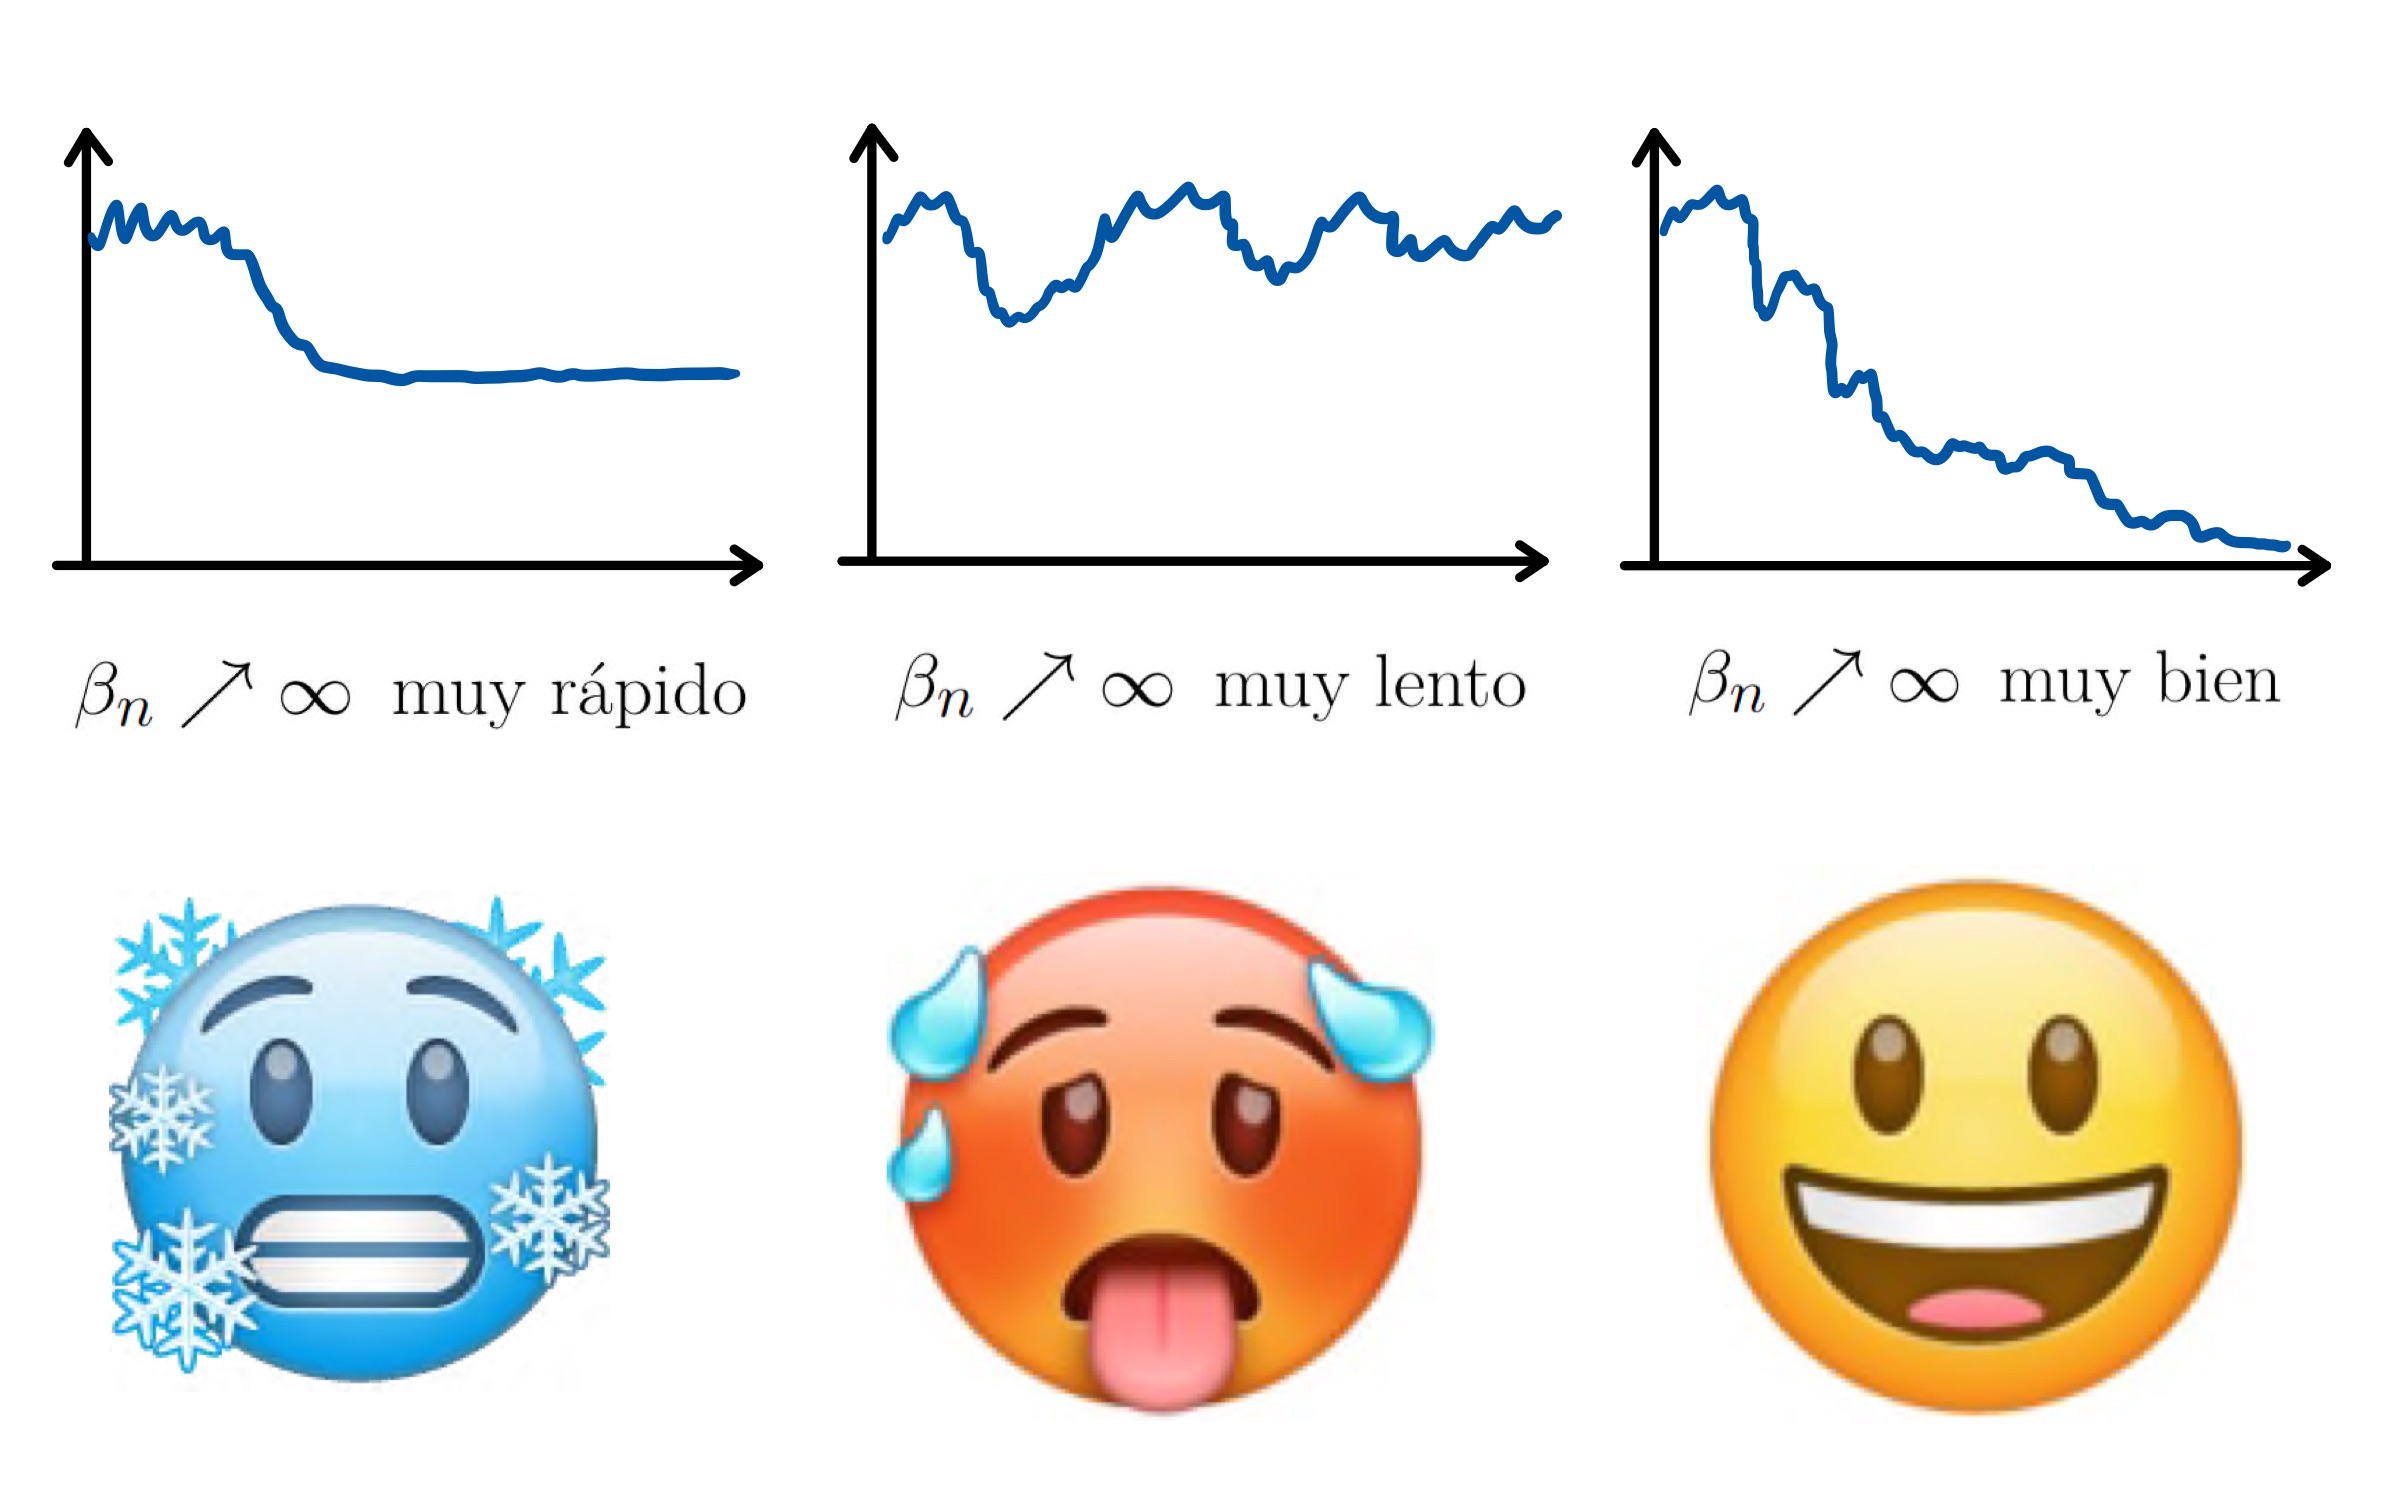
\includegraphics[scale=0.16]{img/clase_14_pag_12.jpg}
    \caption{Idea del efecto de las sucesiones $\beta_n$ en la minimización de la energía $U$.}
    \label{fig:betas}
\end{figure}

% \newpage
\subsection{MCMC y estadística Bayesiana}
\subsubsection{Recuerdo de estadística Bayesiana}
\textbf{Idea}: modelamos simultaneamente y probabilisticamente:
\begin{itemize}
    \item Observaciones $x$ de un fenómeno o dato aleatorio, cuya ley ``$p(x|\theta)$'' depende de un parámetro $\theta\in\Theta$.
    \item La incertidumbre, desconocimiento o conocimiento parcial de $\theta$, lo que representamos asumiendo que $\theta$ es aleatorio y sólo conocemos su distribución ``$p(\theta)$'' ``a priori''.
    \item En lo anterior, la observación $x$ está en un conjunto $\mathfrak{X}$ que puede ser subconjunto de $\R^d$, un conjunto finito o numerable, etc. 
    \newline En general $x\mapsto p(x|\theta)$ (ley de $x$ dado $\theta$) es
    \begin{itemize}
        \item o bien una función de masa discreta: 
        $$\displaystyle\sum_{x\in \mathfrak{X}}p(x|\theta)=1$$
        \item o bien una densidad de probabilidad: 
        $$\displaystyle\int_{\mathfrak{X}}p(x|\theta)dx=1\,.$$
    \end{itemize}
    \item $x$ puede ser una ``muestra'' $x=(x_1,\dots,x_n)$.
    \item $\Theta$ puede ser subconjunto de $\R^k$, conjunto finito o numerable y $p(\theta)$ denota, seg\'un corresponda:
    \begin{itemize}
        \item una función de masa discreta
        \item o bien una densidad de probabilidad,
    \end{itemize}
    con respecto a $\theta$,  y se le llama \textbf{ley a priori}.
    \item $p(x,\theta):=p(x|\theta)p(\theta)$ es ley conjunta en $\mathfrak{X}\times \Theta$ del parámetro y una observación.
    \newline Notar que
    $$ \displaystyle\int_\Theta\int_\mathfrak{X} p(x,\theta)dxd\theta=\int_\Theta\int_\mathfrak{X} p(x|\theta)dx p(\theta)d\theta=1\,.$$
    \item Dado $\theta\in\Theta$, $x\mapsto p(x|\theta)$ se llama ley de $x$ dado $\theta$, o bien la densidad de $x$ condicional a $\theta$.
    \item Dado $X\in\mathfrak{X}$ observación, $\theta\mapsto L(\theta)=L_X(\theta)=p(X|\theta)$ se llama \textbf{función de verosimilitud} (likelihood). Notar que $\int L(\theta)d\theta\neq1$ en general.
\end{itemize}
\textbf{Objetivo de la inferencia Bayesiana}: ``Re-estimar'' el parámetro $\theta$ (modificar o actualizar la ley que describe lo que sabemos de $\theta$) usando la información que nos da el observar $x$.
\begin{theorem}[Bayes]
La ley de $\theta$ dado $x$, también llamada ley posterior de $\theta$, está dada por:
\begin{alignat*}{2}
    p(\theta|x) & := \displaystyle \frac{p(x,\theta)}{p(x)}\\
     & = \displaystyle\frac{p(x|\theta)p(\theta)}{p(x)} \,,
\end{alignat*}
con $p(x)=\displaystyle\int_\Theta p(x,\theta)d\theta$ ley marginal (no condicional).


\end{theorem}
Luego $p(\theta|x)\propto p(x|\theta)p(\theta)$. De esta forma,   $p(x)$ aparece  sólo como una constante de normalización, dependiente de la observaci\'on $x$, cuyo c\'alculo requiere en general sumar o integrar sobre todo el espacio. Por ello,    \textbf{calcular la constante de normalizaci\'on  $p(x)$ puede ser muy costoso,   y hay  evitar tener que hacerlo}.  Es por este motivo que los m\'etodos MCMC son muy \'utiles en este contexto, como veremos un poco m\'as adelante. 
\subsubsection{Aplicaciones de estadística Bayesiana}
\begin{itemize}
    \item Observamos $x_!,\dots,x^n \iid \sim p(x|\theta)dx$ con $\theta$ fijo.
    \newline Sean $\mathcal{D}=\{x_1,\dots,x_n\}$ ``datos'' y su densidad conjunta dada por:
    $$ p(\mathcal{D}|\theta):=p(x_1,\dots,x_n|\theta)=\displaystyle\prod^n_{i=1}p(x_i|\theta)\, . $$
    Además,  consideramos su función de verosimilitud:
    $$ L_\mathcal{D}(\theta)=L_{x_1,\dots,x_n}(\theta)=\displaystyle\prod^n_{i=1}L_{x_i}(\theta)$$
    \item Luego la ley a posteriori de $\theta$ dados $\mathcal{D}$ es la ley en $\Theta$: $$\mathcal{D}=p(\theta|x_1,\dots,x_n)=\displaystyle\frac{\prod^n_{i=1}p(x_i|\theta)p(\theta)}{p(\mathcal{D})}\propto \prod^n_{i=1}p(x_i|\theta)p(\theta)\,$$
    donde la última expresión es evaluable.  $p(\mathcal{D})$ es la densidad marginal de los datos y requiere integrar:
    $$ \displaystyle \int_\Theta p(\mathcal{D}|\theta)p(\theta)d\theta=\int_\Theta\prod^n_{i=1}p(x_i|\theta)p(\theta)d\theta\,.$$
    \item En base a $p(\theta|\mathcal{D})=p(\theta|x_1,\dots,x_n)$, finalmente se construye un ``\textbf{posterior predictivo}'', i.e., un valor $\hat{\theta}_n\in\Theta$ (``estimador de $\theta$'') que mejor explica los datos $x_1,\dots,x_n$.
\end{itemize}
\vspace{1cm}\\
\subsubsubsection{Ejemplos de estimadores Bayesianos}
Los siguiente son estimadores Bayesianos clásicos (hay muchos otros):
\begin{itemize}
    \item \textbf{Media a posteriori}
    \newline Considera  como estimador predictivo la media con respecto a la ley a posteriori de $\theta$.
    $$ \hat{\theta}_n = \displaystyle\int_\Theta p(\theta|\mathcal{D})d\theta\,.$$
    \item \textbf{Máximo a posteriori}
    \newline Es un par\'ametro cuyo  valor  maximiza la probabilidad a posteriori de observar la data $\mathcal{D}$
    \begin{alignat*}{2}
        \hat{\theta}_n & := \displaystyle\arg\max_{\theta} p(\theta|\mathcal{D})\\
         & = \arg\max_{\theta}[\sum^n_{i=1}\log p(x_i|\theta)+\log p(\theta)]\,.
    \end{alignat*}
    En la práctica, la maximización se lleva a cabo como en la última expresión.
\end{itemize}
\begin{remark}
\beforeitemize
\begin{itemize}
    \item También es posible construir regiones o \textbf{regiones o intervalos de confianza} para $\theta$, es decir (para $\theta$ real), un intervalo $I$ tal que $\P(\theta\in I | X_1,\dots,X_n)\approx 95\%$ (por ejemplo).
    \item Se requiere ``conocer'' $p(\theta|\mathcal{D})$ para optimizar en $\theta$ o bien para integrar $p(\theta|\mathcal{D})$ con respecto a $\theta$. En algunos (pocos) casos, $p(\theta|\mathcal{D})$ tiene forma analítica explícita.
\end{itemize}
\end{remark}
%\begin{example}
%\beforeitemize
%\begin{itemize}
%    \item Una moneda... %clase 15 min 48 pag8-9
%\end{itemize}
%\end{example}
\subsubsection{Uso de MCMC}
En general $p(\theta|x_1,\dots,x_n)=\displaystyle \prod^n_{i=1}p(x_i|\theta)p(\theta)$ no tiene forma cerrada.
\newline Además para tener su valor numérico, se requiere integrar $\int\prod^n_{i=1}p(x_i|\theta)p(\theta)d\theta=p(x_1,\dots,x_n)$, lo cual puede ser muy costoso.
\newp \textbf{Idea}: samplear de
\begin{alignat*}{2}
    \Pi(\theta) & := p(\theta|x_1,\dots,x_n)\\
     & = \displaystyle \frac{\prod^n_{i=1}p(x_i|\theta)p(\theta)}{p(\mathcal{D})}\,
\end{alignat*}
usando MCMC en $\Theta$, pues con este m\'etodo \textbf{no se requiere conocer ni calcular $p(\mathcal{D})$, y 
basta poder evaluar rápidamente $\prod^n_{i=1}p(x_i|\theta)p(\theta)$}. La cadena de Markov construida con MCMC vive en $\Theta$ y tiene distribución invariante $$\Pi(\theta)\propto\displaystyle\prod^n_{i=1}p(x_i|\theta)p(\theta)\,.$$  
Cabe notar que: 
\begin{itemize}
    \item el m\'etodo puede aplicarse tanto para $\Theta$ discreto como $\Theta=\R^k$ (usando ``paseo aleatorio en $\R^k$ como cadena Markov de base''). %algo más pag 11
    \item la simulación es costosa en general, sobretodo si el espacio de parámetros tiene dimensión muy grande (se requiere correr muchas veces la cadena de MCMC, por mucho tiempo).
\end{itemize}


\newpage
\section{Algoritmos estocásticos en aprendizaje de máquinas}
Esta unidad estará dedicada a la exploración de algoritmos tipo \textbf{gradiente estocástico}. Si bien los conceptos han sido introducidos hace tiempo, su uso ha subido significativamente en años recientes gracias a su uso en iteligencia artificial y aprendizaje de máquinas. Más precisamente, estos métodos son utilizados para el entrenamiento de redes neuronales profundas, cuyo caso de uso será también introducido en esta sección.

\subsection{Introducción}
Observamos  $\samples\in\R^d\times\R$ muchos datos (potencialmente infinitos) de dimensión (posiblemente) grande.
\begin{example}[Clasificación de imágenes]
Tenemos un conjunto de imágenes, cada una con una etiqueta. Por ejemplo, la foto de un gato, como se grafica en figura \ref{fig:gato}\footnote{Fuente: \url{https://dongminlee.tistory.com/18}}, puede representarse como un vector al ``aplanar'' la matriz correspondiente a la imagen. Las distintas $k$ clases posibles pueden enumerarse de modo que al concepto \textit{gato} se le asigna un número $y\in\{1,\dots,k\}\subset\N\subset\R$.
\begin{figure}
    \centering
    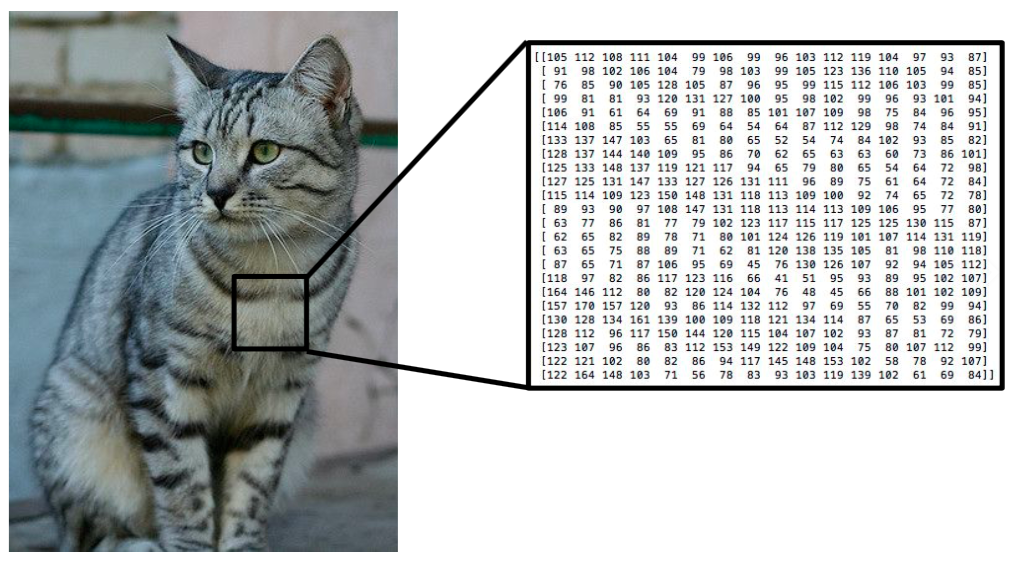
\includegraphics[scale=0.32]{img/figura_gato.png}
    \caption{Imagen con etiqueta ``gato''.}
    \label{fig:gato}
\end{figure}
De este modo, dado un elemento $i$ de nuestros $n$ datos, $x_i\in\R^d$ es un vector que representa la imagen, mientras que $y\in\{1,\dots,k\}$ corresponde a una etiqueta.
\end{example}
\newp \textbf{Objetivo}: aprender de los datos, i.e., aprender a predecir, al ver un $x$ nuevo, la etiqueta $y$ correspondiente.
\begin{example}[Redes Neuronales]
\label{ejemplo:red_neuronal}
Se busca predecir $y$ mediante
% $$ \hat{y}(x,\theta) = \displaystyle \frac{1}{N}\sum^N_{j=1}\sigma_*(x_j,b_j) \,.$$
$$ \hat{y}(x,\theta) = \displaystyle\sum^N_{j=1}\sigma_*(x_j,\theta_j) \,.$$
donde:
\begin{itemize}
    % \item $\sigma_*:\R^d\times\R^D\to\R$ se llama función de activación.
    \item $N$ es el número de neuronas.
    \item $\theta=(\theta_1,\dots,\theta_N)\in(\R^D)^N$ son los parámetros (``pesos'').
    \newline En general, para $j=1,\dots,N$ tomamos $\theta_j=(a_j,b_j,\omega_j)\in \R\times\R\times\R^D $ y $\sigma_*$ de la forma
    $$ \sigma_*(x,\theta_j)=a_i\sigma(\langle x,\omega_i\rangle+b_i) \,.$$
\end{itemize}
\textbf{¿Como aprende?}
\begin{itemize}
    \item Consideramos $l:\R\times\R\to\R_+$ función de pérdida.
    \newline Ej: $l(y,\hat{y})=(y-\hat{y})^2$
    \item Idealmente, buscamos
    $$ \hat{\theta}=\displaystyle\arg\min_\theta \sum^M_{i=1}l(y_i,\hat{y}(x_i,\theta))\,,$$
    con $M$ grande.
    \item Primera idea: aplicar un algoritmo de optimización para ``entrenar la red'' con los datos conocidos. Es decir, encontrar $\hat{\theta}$ óptimo (o casi).
\end{itemize}
\textbf{Problemas}:
\begin{itemize}
    \item Función objetivo costosa de evaluar, debido a una o varias de las razones siguientes:
    \begin{itemize}
        \item $M$ es grande
        \item $d$ es grande, donde $d$ es la dimensión de $x_i$.
        \item $N$ es grande
    \end{itemize}
    \item Requiere tiempo y memoria computacionales (se requiere usar toda la información en todos los pasos).
    \item Sobreajuste (overfitting): Si entrenamos ``perfectamente'' usando todos los $\samples$ (mínimo global) sobreajustamos y perdemos la ``capacidad de generalización''.
\end{itemize}
\textbf{Segunda idea}: Supongamos $(x_i,y_i)\sim\iid$ de ley $\mu$ no conocida.
\newline En vez de buscar
\begin{alignat*}{2}
        \hat{\theta} & = \displaystyle\arg\min_\theta\sum^M_{i=1}l(y_i,\hat{y}(x_i,\theta)) \\
         & = \arg\min_\theta \frac{1}{M}\sum^M_{i=1}l(y_i,\hat{y}(x_i,\theta), 
    \end{alignat*}
buscamos
$$ \hat{\theta}=\displaystyle\arg\min_\theta \E(l(y,\hat{y}(X,\theta)))$$
con $(X,Y)\sim\mu$.
\newp \textbf{¿Tiene sentido?, ¿de qué sirve si no conocemos $\mu$? ¿qué cambia?}
\end{example}
\vspace{1cm}\\
\subsection{Algoritmo de gradiente estocástico}
El descenso de gradiente estocástico (o \textit{S.G.D.} por sus siglas en inglés) es uno de los pilares del desarrollo reciente del aprendizaje de máquinas y de la inteligencia artificial.
\newp Bibliografía: \textit{Stochastic Approximation} (Robbins \& Monro) \cite{robbins}...... Referencia m\'as actual: \textit{Online Learning and Stochastic Approximations} \cite{bottou}.

\subsubsection{El algoritmo}
Consideramos el problema
$$ \min_\theta \E(f(\theta,X)) \, ,$$
con:
\begin{itemize}
\item $f:\R^d\times \R^k\to\R$
    \item $X\sim\mu$
    \item $(\gamma_t)_{t\in\N}$ pasos o tasa de aprendizaje (\textit{learning rate})
\end{itemize}
 Asumiremos en lo que sigue que $f$ es tal que $F(\theta):= \E(f(\theta,X))$ est\'a bien definida, y que se cumple la relaci\'on $\nabla F(\theta)=\E(\nabla_\theta f(\theta,X)) $ para todo $\theta$.
 
En vez de usar un algoritmo gradiente usual $\theta^{t+1}=\theta^t-\gamma_{t+1}\nabla F(\theta^t)=\theta^t-\gamma_{t+1}\E(\nabla_\theta f(\theta^t,X))$, con $(\gamma_t)_{t\in\N}$ sucesión en $\R_+$ pasos, la idea ser\'a \textbf{considerar observaciones} $x_1,x_2,\dots,x_t \iid \sim\mu$ y el algoritmo definido por las iteraciones: 
$$ \theta^{t+1}:=\theta^t-\gamma_{t+1}\nabla_\theta f(\theta^t,x_{t+1})\,.$$
\begin{remark}
\beforeitemize
\begin{itemize}
    \item El término $\nabla_\theta f(\theta^t,x_{t+1})$ se puede ver como un gradiente exacto perturbado por cierto ruido aleatorio, m\'as precisamente, 
    $$ \nabla_\theta f(\theta^t,x_{t+1})=\E(\nabla_\theta f(\theta^t,X))+\Delta_{t+1}=\nabla F(\theta^t)+\Delta_{t+1},$$
    con $\Delta_{t+1}=\nabla_\theta f(\theta^t,x_{t+1})-\E(\nabla_\theta f(\theta^t,X))$  v.a. centrada. 
    \item En cada paso necesitamos evaluar una sola vez $\nabla_\theta f$ (en un solo dato nuevo).
    \item Podemos usar los datos a medida que llegan.
    \item \textbf{Caso particular importante (literatura de optimización)}
    \newline Se quiere optimizar $\tilde{F}(\theta):=\displaystyle\sum^M_{i=1}\tilde{f}_i(\theta)$, con $\tilde{f}_i:\R^d\to\R$ ($M$ funciones), lo cual es equivalente a
    % \newline $\ssi$ 
    optimizar $F(\theta)=\displaystyle\frac{1}{M}\sum^n_{i=1}\tilde{f}_i(\theta)=\E(f(I,\theta))$ con $I=X\sim \frac{1}{M}\sum^M_{i=1}\delta_i$ (esto es,  $I\in\{1,\dots,M\}$ es un índice  aleatorio  elegido de manera uniforme), y $f(i,\theta)=\tilde{f}_i(\theta)$.  Entonces, 
    $$ \theta^{t+1}:=\theta^t-\gamma_t \nabla_\theta f(\theta^t,I_{t+1})=\theta^t-\gamma_t \nabla_\theta\tilde{f}_{I_{t+1}}(\theta), $$
    con $I_1,I_2,\dots \iid\sim\mathbb{U}(\{1,\dots,M\})$.
\end{itemize}
\end{remark}
El siguiente es un enunciado cl\'asico sobre este tipo de algoritmo, que damos inicialmente sin todos los detalles: 
\begin{theorem}[Sigmund, Robbins, (1951)] 
Bajo hipótesis razonables sobre $f$ (regularidad en $\theta$, integrabilidad de $\nabla_\theta f_+$, cotas), si $\gamma_t\,\substack{\searrow \\ \tiny{t\to\infty}}\, 0$ suficientemente lento la sucesión:
$$ \theta^t\mbox{ }\overset{c.s.}{\substack{\longrightarrow \\t \to \infty}}\mbox{ }\mbox{ Conjunto de puntos críticos de } F(\theta)=\E(f(\theta,X)).$$
Más aún, si $f$ es convexa,  estrictamente en $\theta$ (más algunas hipótesis adicionales), entonces
$$ \theta^t\mbox{ }\overset{c.s.}{\substack{\longrightarrow \\t \to \infty}}\mbox{ }\arg\min_\theta \E(f(\theta,X))\,.$$
\end{theorem}
\begin{remark}

Si bien este tipo de resultados fueron obtenidos por primera vez hace cerca de 70 años, la utilizaci\'on del descenso de gradiente estocástico (o \textit{S.G.D.}  ha sido fuertemente reimpulsada con el desarrollo reciente  del aprendizaje de máquinas y de la inteligencia artificial pues, entre otros motivos, los siguientes: 
\begin{itemize}
    \item Permite ``entrenar'' (estimar) parámetros con datos,  a medida que estos  van llegando.
    \item Permite ``actualizar'' la estimación en tiempo real (a medida que llegan nuevos datos).
    \item Es ``escalable'': el costo es temporal (uso de memoria constante) y proporcional al tamaño del conjunto de datos.
    \item Si bien no está garantizada la convergencia a un óptimo global, muchas veces permite encontrar un mínimo local $\hat{\theta}=\theta^t$ que ``generaliza bien'' (como estimador) en el sentido siguiente:  si $t$ es suficientemente grande,  $X_1,\dots,X_t$ es el conjunto de entrenamiento,  y  $X_{t+i}, i=0,\dots, N$ son datos nuevos,  entonces
    $$ \displaystyle\frac{1}{N}\sum^N_{i=1}f(\theta^t,X_{t+i})\mbox{ es cercano a }\E(f(\theta^t,X)) \mbox{ y } \E(f(\theta^t,X)) \mbox{ es cercano a } \min_\theta \E(f(\theta,X)). $$
\end{itemize}
\end{remark}
   
\begin{remark} Desde el punto de vista pr\'actico: 
\begin{itemize}
\item Típicamente, se buscan mínimos locales ``buenos'', de valores cercanos al global, pero no necesariamente un m\'inimo global.
    \item Se sugiere correr el algoritmo desde muchos $\theta_0$ iniciales y guardar el mejor valor obtenido.
    \item Se sugiere probar adem\'as distintas elecciones de paso $\gamma_t$ y guardar la que de mejores resultados. En la práctica se suele usar $\gamma_t=$constante o constante por tramos ($t$ no tiende a infinito en la vida real)
    \item Hay muchas variantes para acelerar ``convergencia'' o bien para explorar mejor el espacio. Un ejemplo de eso \'ultimo es agregar ``ruido'' o aleatoriedad adicional,  para evitar quedar atrapado en  mínimos locales malos.
    \end{itemize}
\end{remark}
\begin{notation}
En lo que sigue, denotamos $\partial f(\theta,x)=\nabla_\theta\,.
\end{notation}
\subsubsection{Convergencia en el caso convexo}

Para probar la convergencia en el caso convexo necesitaremos herramientas de cálculo estocástico.
\begin{definition}[Martingala]
Sea $(\Omega,\mathcal{F},\P)$ un espacio de probabilidad dotado de una filtración $(\mathcal{F}_t)_{t\in\N}$ (i.e., $\sigma$-álgebras tal que $\forall t\in\N$, $\mathcal{F}_t\subset\mathcal{F}_{t+1}\subset\mathcal{F}$).  Una familia de variables aleatorias se dice martingala si
$$ X_t\in L^1(\mathcal{F}_t) \forall t\in\N$$ y $$\forall t\in\N\espacio \E(X_{t+1}|\mathcal{F}_t)=X_t  \mbox{ c.s.}$$
\begin{notation}
Si en la última ecuación tenemos $\geq$ en vez de igualdad entonces la familia se dice \textbf{sub-martingala}. Si tenemos $\leq$ entonces la llamamos \textbf{sobre-martingala}.
\end{notation}
\end{definition}
En particular usaremos el siguiente teorema del curso de cálculo estocástico, que asumiremos sin demostración.
\begin{theorem}[Convergencia sobre-martingalas]
\label{theorem:sobre-m}
Sea $(X_t)_{t\in\N}$ una sobre-martingala con respecto a $(\mathcal{F}_t)_{t\in\N}$ tal que $\displaystyle\sup_{t\in\N}\E(X_t^-)<\infty$. Entonces $\exists X_\infty\in L^1$ tal que $$ X_t\convcst X_\infty \,.$$
\end{theorem}
\begin{theorem}[Descenso de gradiente estocástico caso convexo]
\label{teo:sgd}
Supongamos que los datos ....  son v.a. i.i.d. de ley $\mu$ definas en un espacio de probabilidad $(\Omega,\mathcal{F},\P)$.  Adem\ás, supongamos que:  
\begin{itemize}
    \item[i)] $\forall \theta\, , f(\theta,\cdot)\in L^1(\mu). \mbox{ Adem\'as }  $f(\cdot,x)\in\mathcal{C}^1 \mu(dx)-c.s.$,  \mbox{ y } $\partial_\theta f(\theta,\cdot)\in L^1(\mu)$
    \item[ii)] $F$ tiene un único mínimo $\theta^*$
    \item[iii)] $\forall \epsilon >0$, $\displaystyle \inf_{\theta:\|\theta-\theta^*\|^2>\epsilon}(\theta-\theta^*)\nabla F(\theta)>0$
    \newline i.e., lejos de $\theta^*$, $F$ decrece estrictamente, uniformemente hacia $F(\theta^* )$
    \item[iv)] $\exists A,B\geq 0$ tal que $\E(\|\partial f(\theta,X)\|^2)\leq A+B\|\theta-\theta^*\|^2, \forall \theta$
    \item[v)] $\sum_{t\in\N}\gamma_t=\infty$, $\sum_{t\in\N}\gamma_t^2<\infty$ \espacio (por ejemplo: $\gamma_t=\frac{1}{t}$).
\end{itemize}
Entonces
$$ \theta_t\mbox{ }\overset{c.s.}{\substack{\longrightarrow \\t \to \infty}}\mbox{ }\theta^*\,.$$

\end{theorem}
\begin{remark}
\beforeitemize
\begin{itemize}
\item (i) $\implies F\in\mathcal{C}^1(\R^d)$ con  $\nabla F=\E(\partial_\theta f(\theta,x))$. 
     \item Si bien no pedimos explícitamente que la función $F$ sea  convexa, haciendo un Taylor en $\theta$ se puede verificar que las hipótesis ii) y iii) se cumplen, si  $F$ es  de clase ${\cal C}^2$ y estrictamente convexa. 
     \item (iii)  impide que el gradiente se ``aplane'' lejos del m\'inimo global. 
    \item (iv) se cumple si por ejemplo $f(\cdot,x)$ es  de clase ${\cal C}^2$ con  $\E(\|Hess_\theta f(\theta,X)\|)<\infty$ % . TERMINAR LA REMARK
\end{itemize}
\end{remark}
\begin{proof}[Demostración de Teorema \ref{teo:sgd} descenso de gradiente estocástico, caso convexo]
\gris \\ Tomemos la función  siguiente como “funci\'on de de Lyapunov" :
$$ h(\theta) = \|\theta-\theta^*\|^2\, , $$
y denotemos $h_t:=h(\theta_t)$. Queremos probar que $h_t$ converge a $0$ c.s., con lo cual tendremos que $\theta_t\mbox{ }\overset{c.s.}{\substack{\longrightarrow \\t \to \infty}}\mbox{ }\theta^*$. En efecto,
$$ \theta_{t+1}-\theta^* = \theta_t-\theta^*-\gamma_t\partial f(\theta_t,x_{t+1}) \,.$$
Luego aplicando $\|\espacio\|^2$,
$$ \|\theta_{t+1}-\theta^*\|^2 = \|\theta_t-\theta^*\|^2-2\gamma_t(\theta_t-\theta^*)\partial f(\theta_{t},x_{t+1})+\gamma^2_t\|\partial f(\theta_t,x_{t+1})\|^2 \,,$$
entonces
$$ h_{t+1}-h_t = -2\gamma_t(\theta_t-\theta^*)\partial f(\theta_t,x_{t+1})+\gamma_t^2\|\partial f(\theta_t,x_{t+1})\|^2 \, .$$
Ahora haremos aparecer una sobre-martingala. Tomemos como filtración la tribu generada por las observaciones, i.e.,$ (\mathcal{F}_t=\sigma(x_0,\dots,x_t))_{t\in\N}$, asumiendo adem\'as que la condici\'on inicial $\theta_0$ es determinista. 

Por inducci\'on se ve f\'acilmente  que  $\theta_t\in L^2(\Omega,\mathcal{F},\P)\,\forall t\in\N$, gracias a la condici\'on iv). Tomando esperanza condicional respecto a $\mathcal{F}_t$:
$$ \E(h_{t+1}-h_t|\mathcal{F}_t)  = -2\gamma_t(\theta_t-\theta^*)\E(\partial f(\theta,X))\big\vert_{\theta = \theta_t}  +\gamma_t^2\E(\|\partial f(\theta,X)\|^2)\big\vert_{\theta = \theta_t} \,,$$
donde usamos que $x_{t+1}\indep \mathcal{F}_t$, con lo cual $\E( G(\theta_t,x_{t+1})|\mathcal{F}_t)) = \E(G(\theta,X))\vert_{\theta = \theta_t}$ para toda $G$ apropiada. Además, por (iv),  $\exists A,B\geq 0$ tal que $\E(\|\partial f(\theta,X)\|^2)\big\vert_{\theta = \theta_t} \leq A+B\|\theta_t-\theta^*\|^2$, por ende
$$ \E(h_{t+1}-h_t|\mathcal{F}_t) \leq -2\gamma_t(\theta-\theta^*)\E(\partial f(\theta,X))\big\vert_{\theta=\theta_t} +A\gamma_t^2+B\gamma_t^2 h_t \,.$$
Como $h_t$ es $\mathcal{F}_t$-medible, puede entrar en la esperanza condicional del lado izquierdo, con lo cual 
\begin{alignat*}{2}
\E(h_{t+1}-(1+\gamma_t^2 B)h_t|\mathcal{F}_t) & \, \leq \, -2\gamma_t(\theta_t-\theta^*)\nabla F(\theta_t)+\gamma_t^2 A .
\end{alignat*}
 Definimos $\mu_t:=\displaystyle\prod^{t-1}_{k=1}\frac{1}{1+\gamma_k^2B}$ y $h'_t:=\mu_th_t$. Multiplicando por $\mu_{t+1}$ queda que
$$ \E(h'_{t+1}-h_t'|\mathcal{F}_t)\leq -2\gamma_t(\theta_t-\theta^*)\nabla F(\theta_t) + \gamma_t^2A\mu_{t+1}   \, \leq \gamma_t^2A\mu_{t} \,,   $$
donde usamos (iii) y el hecho que $\mu_{t+1}\leq \mu_t $. Notar que $\mu_t \convt \mu_\infty\in(0,\infty)$, como puede verse tomando logaritmo y usando que $\sum\gamma_t^2<\infty$. De la desigualdad anterior deducimos que
$$ X_t:=h_t'-\displaystyle\sum^{t-1}_{k=0}A\gamma_t^2\mu_t$$
es una sobre-martingala con respecto a $(\mathcal{F}_t)_{t\in\N}$, es decir $\E(X_{t+1}|\mathcal{F}_t)\leq X_t\,\forall t\in\N$. Para usar el Teorema \ref{theorem:sobre-m} de convergencia de  sobre-martingalas, veamos que es acotada por debajo. En efecto, como $h_t'\geq 0$, tenemos que 
$$ X_t \geq 0 - \displaystyle A\sum^\infty_{k=0}\gamma_t^2\cdot(\sup_{j\in\N}\mu_j)>-\infty.  $$
Así, por el Teorema de convergencia de  sobre-martingalas, 
 $\exists X_\infty\in L^1$ tal que $X_t\convcst X_\infty$. Dado que 
 $$A\sum^N_{t=1}\gamma_t^2\mu_t \mbox{ }\substack{\longrightarrow \\ N\to\infty}\mbox{ } A\sum^\infty_{t=1}\gamma_t^2\mu_t <\infty, $$ se sigue que
$ h'_t \mbox{ }\overset{c.s.}{\substack{\longrightarrow \\t \to \infty}}\mbox{ } h'_\infty \,,$
para cierta v.a. $ h'_\infty\in L^1$, 
y puesto que $\mu_t \convt \mu_0\in(0,\infty)$, deducimos que $$h_t\mbox{ }\overset{c.s.}{\substack{\longrightarrow \\t \to \infty}}\mbox{ }h_\infty$$ para cierta $h_\infty\in L^1$. 
Para concluir el teorema,  veamos que $h_\infty=0\,c.s.$.  Volviendo a la desigualada satisfecha por $\E(h'_{t+1}-h_t'|\mathcal{F}_t)$, vemos que 
$$ 0\leq 2\mu_t \gamma_t(\theta_t-\theta^*)\nabla F(\theta_t)\leq \gamma_t^2A\mu_t + \E(h'_t-h'_{t+1}|\mathcal{F}_t) \,,$$
de donde
\begin{alignat*}{2}
 2\E(\displaystyle\sum^N_{t=0}\gamma_t\mu_t(\theta_t-\theta^*)\nabla F(\theta_t)) & \leq \displaystyle\sum^N_{t=1}\gamma_t^2 A\mu_t+\E(h_0)-\E(h_{N}) \\
& \leq A\sum^{\infty}_{t=1}\gamma_t^2\mu_t+\E(h_0)<+\infty
\end{alignat*}
$$ \therefore \espacio \displaystyle\sum^\infty_{t=0}\gamma_t\mu_t(\theta_t-\theta^*)\nabla F(\theta_t)<\infty \espacio c.s.\,.$$
Puesto que $\mu_t\convt\mu_\infty\in(0,\infty)$, $\mu_t$ est\'a acotada por debajo lejos de $0$, por lo que 
$$  \displaystyle\sum_t\gamma_t(\theta_t-\theta^*)\nabla F(\theta_t)<\infty \, c.s.\,.$$
Usando (v),\espacio $\displaystyle\sum_t\gamma_t=\infty$, con lo cual necesariamente se cumple que 
$$ \displaystyle\liminf_{t\to\infty}(\theta_t-\theta^*)\nabla F(\theta_t) = 0 \,c.s.\,.$$
Para concluir, consideremos $\Omega'_\epsilon=\{h_\infty>\sqrt{\epsilon}\}$ y supongamos que $\P(\Omega'_\epsilon)>0$. Usando (iii) tenemos que $\P(\displaystyle\liminf_{t\to\infty}(\theta_t-\theta^*)\nabla F(\theta_t)>0)\geq \P(\Omega'_{\epsilon/2})  >0$, que es una contradicción. 
$$ \therefore\espacio \P(\Omega'_\epsilon)=0\espacio\forall\epsilon>0,\espacio \Longrightarrow\espacio h_\infty=0\espacio c.s.\,. $$ \findem
\negro
\end{proof}
\vspace{1cm}\\
\subsubsection{Convergencia en caso no-convexo}
\begin{theorem}[Extensión de Descenso de gradiente estocástico (caso no-convexo)]
\label{theorem:sgd_no_conv}
Supongamos:
\begin{itemize}
    \item[i)] $f(\theta,\cdot)\in L^1(\mu)$, $f(\cdot,x)\in\mathcal{C}^3,  \mu(dx)-c.s.$, $\partial^k f(\theta,\cdot)\in L^1(\mu), k=1,2,3$ (luego $F\in\mathcal{C}^3$)
    \item[ii)] $F$ es acotada por debajo
    \item[iii)] $\exists A_k,B_k\geq 0$ tal que $\E(\|\partial f(\theta,X\|^k)\leq A_k+B_k\|\theta\|^2,\espacio k=1,2,3$
    \item[iv)] $\forall M >0$, $\displaystyle \inf_{\theta:\|\theta\|^2>M}\theta\nabla F(\theta)>0$
    \item[v)] $\sum_{t\in\N}\gamma_t=\infty$, $\sum_{t\in\N}\gamma_t^2<\infty$
\end{itemize}
Entonces tenemos lo siguiente (casi seguramente):
\begin{itemize}
    \item[a)] $(\theta_t)_{t\in\N}\subset \mbox{ un compacto }\R^d$
    \item[b)] $\exists F_\infty \in L^1 \mbox{ tal que }F(\theta_t)\convcst0$
    \item[c)] $\nabla F(\theta_t)\convcst 0$
\end{itemize}
\end{theorem}

\begin{remark}
\beforeitemize
\begin{itemize}
    \item El resultado no implica convergencia c.s. de $(\theta_t)_{t\in\N}$\,.
    \item (a)$\implies$ toda subsucesión tiene una subsucesión convergente c.s. $\theta_{t_k}\mbox{ }\substack{\longrightarrow \\ k\to\infty}\mbox{ } \tilde{\theta}$
    \newline (b), (c) $\implies$ por continuidad de $F$ y $\nabla F$,
    $$F(\theta_{t_k})\mbox{ }\substack{\longrightarrow \\ k\to\infty}\mbox{ }F(\tilde{G})\espacio\land\espacio \nabla F(\theta_{t_k})\mbox{ }\overset{c.s.}{\substack{\longrightarrow \\k \to \infty}}\mbox{ }0=\nabla F(\tilde{\theta})\,.$$
    \newline $\therefore\mbox{ si }Crit:\{\theta:\nabla F(\theta)=0\}$, $\forall \epsilon>0$, $\P(dist(\theta_t,Crit)>\epsilon)\mbox{ }\substack{\longrightarrow \\ t\to\infty}\mbox{ }0$\espacio, i.e., la probabilidad de estar a distancia positiva de puntos críticos tiende a $0$.
\end{itemize}
\end{remark}
% \vspace{.75cm}\\
\begin{proof}[Esquema de Demostración de Teorema \ref{theorem:sgd_no_conv}, gradiente estocástico, caso no-convexo]
\gris 
% Veremos un esquema de demostración. 
Para más detalles ver Bottou et al. \cite{bottou}.
\newp Usaremos nuevamente el argumento con sobre-martingalas usando una función de Lyapunov ($h(\theta)$). Veremos un confinamiento, o sea que el algoritmo nos llevará a estar en un compacto. Tomamos
$$ h(\theta) = (\|\theta\|^2-M)^2_+=\phi(\|\theta\|^2)\,,$$
donde $\phi(r)=(r-M)_+^2$, y tomamos $h_t:=h(\theta_t)\,\forall t\in\N$. Usando la hipótesis (iii) y un Taylor de orden 1 se demuestra que
$$ \E(h_{t+1}-h_t|\mathcal{F}_t) \leq -2\gamma_t\theta_t\nabla F(\theta_t)\phi'(\|\theta\|^2)+\gamma_t^2(A+Bh_t) \,, $$
con $\phi'(r)=\begin{cases}
0 & r\leq M \\ 2(r-M) & r>M \, .
\end{cases}$ 
\newline Luego por Teorema \ref{theorem:sobre-m}, $h_t\convt h_\infty\in L^1$. Entonces
$$ \displaystyle\sum_{t=0}^\infty\gamma_t\theta_t\nabla F(\theta_t)\phi'(\|\theta_t\|^2)<\infty\espacio c.s. \, , $$
y como por (v) tenemos $\sum\gamma_t=\infty$, necesariamente $\displaystyle\liminf_{t\to\infty} \theta_t\nabla F(\theta_t)\phi'(\|\theta_t\|^2) = 0$. Además, por (iv) $\displaystyle\liminf_{t\to\infty}\phi'(\|\theta_t\|^2)=0\espacio \implies \espacio h_\infty=0\,c.s.\espacio$, $\therefore \|\theta_t\|\leq 2M \espacio c.s.$ para todo $t$ suficientemente grande (aleatorio).
\newp Para demostrar la convergencia de $F(\theta_t)$ usamos un Taylor de orden 1 para obtener 
$$ F(\theta_{t+1})-F(\theta_t)\leq -\gamma_T\partial f(\theta_t,X_{t+1})\nabla F(\theta_t)+\frac{1}{2}\gamma^2_t\|\partial f(\theta_t,X_{t+1})\|^2\partial^2F(\tilde{\theta}_t) \,,$$
luego obtenemos una sobre-martingala al tomar esperanza condicional con respecto a $\mathcal{F}_t$. Luego definiendo $h_t:=F(\theta_t)\espacio(\geq cte)$ se demuestra que
$$ \E(h_{t+1}-h_t|\mathcal{F}_t) \leq -\gamma_t\|\nabla F(\theta_t)\|^2+\gamma_t^2C \,,$$
y nuevamente tenemos que existe $F_\infty\in L^1$ tal que $F(\theta_t)=h_t\convt F_\infty$.

\newp Para la convergencia de $\nabla F(\theta_t)$ a $0$ notemos que
$$ \E(h_{t+1}-h_t|\mathcal{F}_t) \leq -\gamma_t\|\nabla F(\theta_t)\|^2+\gamma_t^2C \espacio \implies \espacio \displaystyle\sum^\infty_{t=1}\gamma_t\|\nabla F(\theta_t)\|^2<\infty \,,$$
con lo cual $\displaystyle\liminf_{t\to\infty}\|\nabla F(\theta_t)\|^2=0$. Para concluir debemos mostrar que $h_t:=\|\nabla F(\theta_t)\|^2$ es convergente. En efecto haciendo un taylor de orden 2 para $\|\nabla F\|^2$ tenemos
$$ \|\nabla F(\theta_{t+1})\|^2-\|\nabla F(\theta_t)\|^2 \leq -2\gamma_t\partial f(\theta,X_{t+1})Hess(F(\theta_t))\nabla F(\theta_t)+\gamma_t^2\|\partial^2 f(\theta,X_{t+1})\| M''' \,,$$
luego
$$ \E(h_{t+1}-h_t|\mathcal{F}_t) \leq 2\gamma_t\|\nabla F(\theta_t)\|^2 +\gamma_t^2M''' \,.$$
Basta notar que tanto $2\gamma_t\|\nabla F(\theta_t)\|^2$ como $\gamma_t^2M'''$ son convergentes, por ende podemos usar nuevamente el Teorema \ref{theorem:sobre-m} para encontrar un $h_\infty$, que necesariamente debe ser $0$ por lo anterior, i.e.,
$$ h_t = \|\nabla F(\theta_t)\|^2\convt 0\,c.s.$$
\findem
\negro
\end{proof}
\begin{remark}[\textbf{Posibilidades a tener en mente}]
% \textbf{Posibilidades a tener en mente}
Al correr el algoritmo podemos encontrarnos en los siguientes casos, graficado en la figura \ref{fig:sgd}.
\begin{itemize}
    \item Mínimo local: Ok, eligiendo el mejor entre muchas corridas.
    \item Máximo local (u otra cosa): Malo, pero fácil de descartar.
    \item Mínimo global: No necesariamente deseable pues se corre el riesgo de sobreajustar. Además es ``inalcanzable''.
    \item Plateau asintótico: Muy malo. No deberia ocurrir bajo la hipótesis (iv).
\end{itemize}
\end{remark}
\begin{figure}
    \centering
    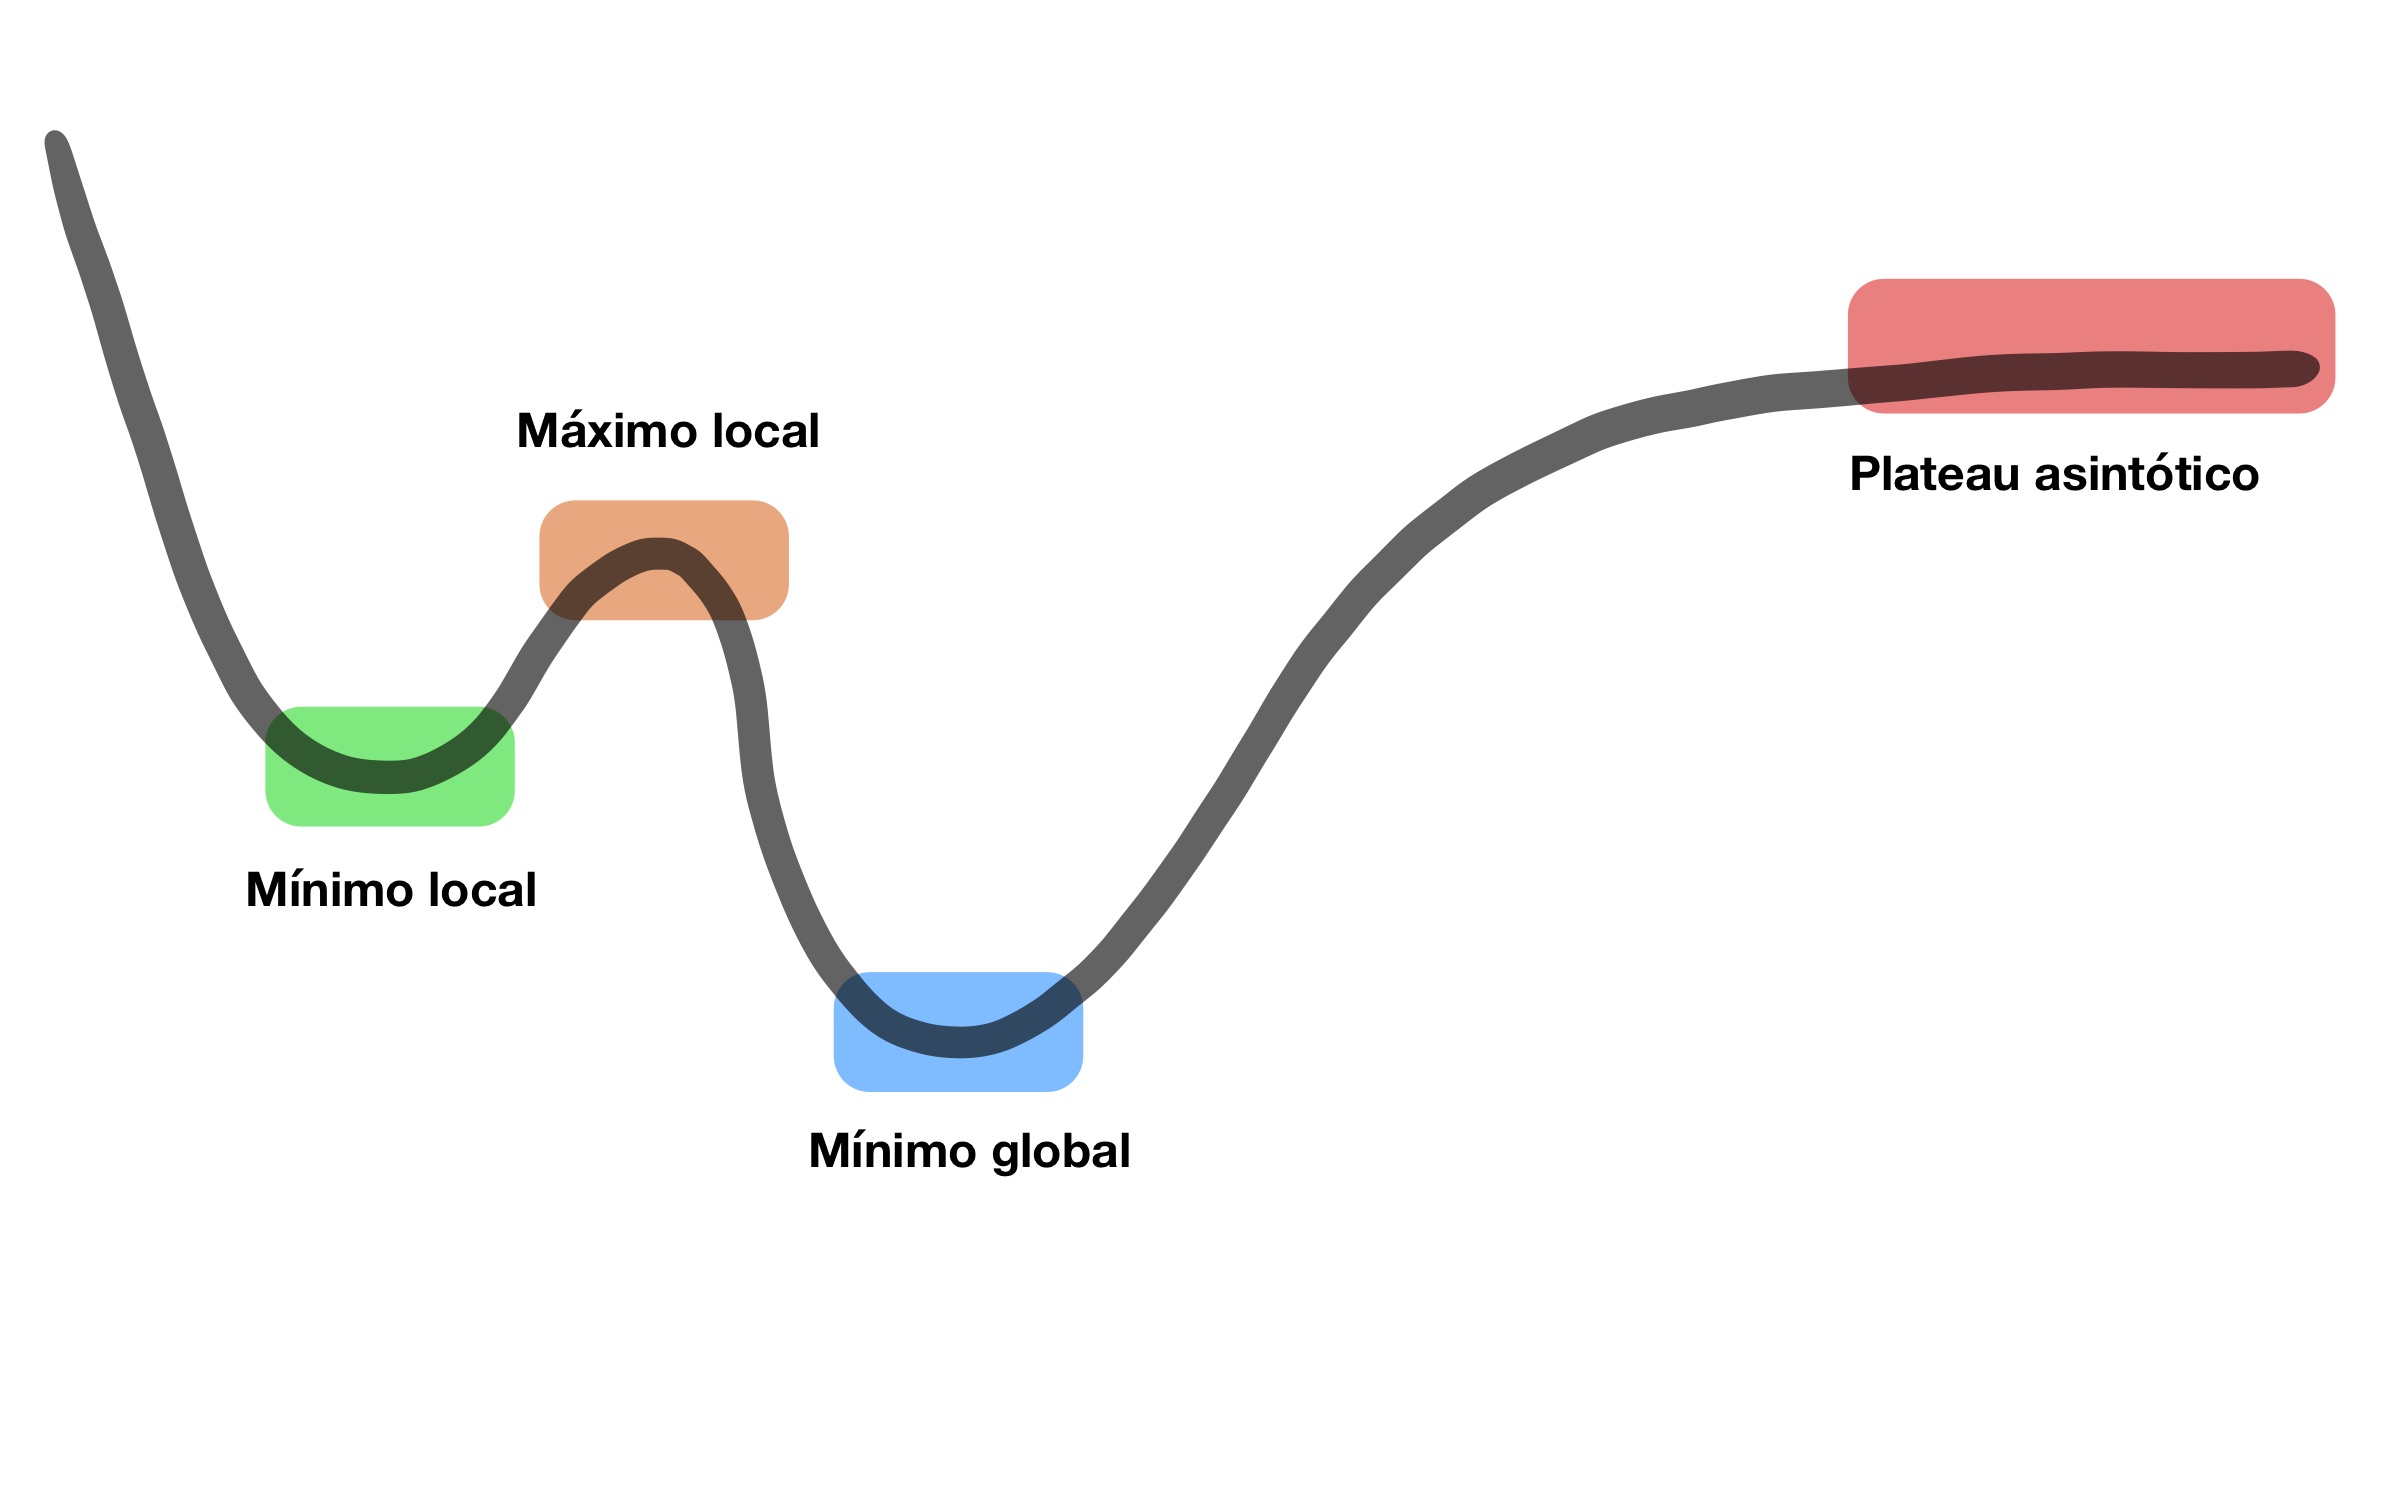
\includegraphics[scale=0.16]{img/Clase_18_pag_09.jpg}
    \caption{Distintos resultados al aplicar S.G.D.}
    \label{fig:sgd}
\end{figure}
% \vspace{1cm}\\
\subsubsection{Tasa de convergencia}
Sobre la tasa de convergencia tenemos las siguientes comparaciones entre descenso de gradiente y descenso de gradiente estocástico:
\newp \textbf{Descenso Gradiente (algoritmo clásico determinista)}
\begin{itemize}
    \item $F$ convexa: $F(\theta_t)-F(\theta^*)=O(\frac{1}{\sqrt{t}})$
    \item Convexa con $\nabla F$ Lipschitz: $F(\theta_t)-\F(\theta^*=O(\frac{1}{t})$
    \item Fuertemente convexa + $\nabla F$ Lipschitz: $F(\theta_t)-F(\theta^*)=O(e^t),\espacio e\in(0,1)$
\end{itemize}
\newp \textbf{Descenso de gradiente estocástico con pasos $\gamma_t\sim \frac{1}{t}$}
\begin{itemize}
    \item $F$ convexa: $F(\theta_t)-F(\theta^*)=O(\frac{1}{\sqrt{t}})$
    \item Convexa con $\nabla F$ Lipschitz: $F(\theta_t)-\F(\theta^*=O(\frac{1}{\sqrt{t}})$
    \item Fuertemente convexa + $\nabla F$ Lipschitz: $F(\theta_t)-F(\theta^*)=O(\frac{1}{t})$
\end{itemize}
\subsection{Variantes de Gradiente Estocástico}
\subsubsection{Gradiente estocástico con Mini-Batch}  % 47:50 clase 18
Es una variante muy utilizada en la práctica. Viene del anglicismo Batch que significa ``lote''.
\newp \textbf{Idea}: en general tenemos
$$ \theta_{t+1}=\theta_t - \gamma_t \partial_\theta f(\theta_t,X_{t+1})=
\theta_t - \gamma_t (\nabla F(\theta_t)+\partial_\theta f(\theta_t,X_{t+1})-\nabla F(\theta_t)\,,$$
donde $\Delta_t=\partial_\theta f(\theta_t,X_{t+1})-\nabla F(\theta_t)$ es aleatorio y lo interpretamos como ruido, con $\E(\Delta_t)=0$. Dicho de otro modo, tenemos un ``gradiente perturbado''.
\newline Notemos que $\partial_\theta f(\theta_t,X_{t+1})$ es un \textbf{estimador insesgado} de $\nabla F(\theta)$. Si tomamos esperanza nos da
$$ \E(\partial_\theta f(\theta_t,X_{t+1}))=\nabla F(\theta_t)\,.$$
Sin embargo también lo es la siguiente expresión, para $m$ fijo:
$$ \displaystyle\frac{1}{m}\sum^m_{i=1}\partial_\theta f(\theta_t,X_{t+i})\,.$$
Más aún, con lo anterior estaremos reduciendo varianza.

\newp \textbf{Descenso de gradiente con mini-batch}:
\newline Sea $m$ fijo (tamaño del mini-batch), y $x_1,\dots,x_t,\dots \iid \sim \mu$, entonces tomamos:
$$ \theta_{t+1}=\theta_t - \gamma_t\cdot \displaystyle\frac{1}{m}\sum^m_{k=1}\partial_\theta f(\theta_t,x_{t+i})$$
con
$$ Var(\displaystyle \frac{1}{m}\sum^m_{k=1}\partial_\theta f(\theta,x_{t+i}))=\frac{Var(\partial_\theta f(\theta,x))}{m}=\frac{\sigma^2}{m}$$
Posee entonces las siguientes ventajas:
\begin{itemize}
    \item El estimador del gradiente posee mucha menos varianza.
    \item Lo anterior implica que hay fluctuaciones más pequeñas.
    \item Aprovecha ``vectorización en computadores'' (GPU, paralelización, ...).
\end{itemize}
\begin{remark}
\beforeitemize
\begin{itemize}
    \item En el caso conexo fuerte con $\gamma_t=\gamma<\frac{2}{\mu}$ se puede probar que
    $$ \E(\|\theta_t-\theta^*\|^2)\leq (1-2 \alpha \mu)^t\|\theta_0-\theta^*\|^2+\frac{\gamma \sigma^2}{m 2\mu}\,,$$
    donde 
    $$ F(\theta)-F(\eta)\geq \nabla F(\theta)(\theta-\eta)+\frac{\mu}{2}\|\theta-\eta\|^2\,.$$
    \item $m$ y $\eta_t$ se deben ajustar conjuntamente.
    \item ``mini-batch'': entre el lote completo de datos (Descenso de gradiente usual) y S.G.D. ``en línea''.
    \item En la práctica, S.G.D. se usa casi siempre con mini-batch, de tamaño fijo $m$ para aprovechar capacidad de cálculo ``paralelo''. El costo de un paso con mini-batch es menor a $m$ por el costo de un paso con un dato.
    \item Tener varianza pequeña no siempre es deseable al comienxo: ayuda a no quedar bloqueado en mínimos locales, por ende tomamos $\gamma_t\searrow$.
    \item Tampoco es necesario ``esperar'' a que las fluctuaciones ``lleguen a $0$'' (con $\gamma_t\to 0$).
    \newline Se puede parar fijando un criterio $|F(\theta_{t_k})-F(\theta_{t_{k+1}})|<\epsilon$\,.
\end{itemize}
\end{remark}

\subsubsection{Más variantes de Gradiente Estocástico}
Existen variantes de descenso de gradiente estocástico que explotan la dinámica determinista subyacente para una convergencia más rápida. Si bien en algunos casos tendremos convergencia, muchas veces estos métodos son heurísticas. Los algoritmos mencionados en esta sección están disponibles en las principales bibliotecas de \textit{python} como \href{https://pytorch.org/docs/stable/optim.html#algorithms}{pytorch}, \href{https://www.tensorflow.org/api_docs/python/tf/keras/optimizers}{tensorflow} y \href{https://mxnet.apache.org/versions/1.7/api/python/docs/tutorials/packages/optimizer/index.html}{Apache MXNet}.
\subsubsubsection{Momentum}
El método momentum utiliza el gradiente de la etapa anterior mediante la siguiente recurrencia:
$$ \theta_{t+1} = \theta_t - \gamma_t m_{t+1} \,,$$
con
$$ m_{t+1}=\beta m_t+(1-\beta)\nabla_\theta f(\theta_t,X_{t+1}), \espacio m_0=0\espacio .$$
Esto mantiene algo de las direcciones de descenso anteriormente usadas (``olvido exponencial'').

\subsubsubsection{AdaGrad}  %1:05
AdaGrad consiste en dividir el paso por un factor proporcional a la norma de los gradientes acumulados hasta entonces.
$$ \theta_{t+1}=\theta_t-\displaystyle \frac{\gamma_t}{\sqrt{v_t+\epsilon}}\nabla_\theta f(\theta,X_{t+1}) \,,$$
para $\epsilon$ fijo y con
$$ v_t = \displaystyle \sum^{t-1}_{k=1}\|\nabla_\theta f(\theta,X_k)\|^2\,,\espacio v_1=0\,.$$
Este método va haciendo que los pasos sean más chicos si hemos dado pasos grandes, evitando salir de buenos mínimos locales. Análogamente, al llegar a una zona plana este factor aumentará, de modo que se pueda salir hacia mejores valores.

\subsubsubsection{Variante Estocástica (Stochastic Gradient Langevin Dynamics)}
La siguiente variante ``agrega estocasticidad'' para explorar de mejor manera el espacio y evitar mínimos locales. Tomamos
$$ \theta_{t+1}=\theta_t-\gamma_t\nabla_\theta f(\theta_t,X_{t+1}) + \beta_t \mathcal{N}_t(0,I_d)\,$$
donde las $ \beta_t\sim \mathcal{N}_t(0,I_d)$ son independientes y representas ruido exógeno. Podemos tomar $\beta_t$ tendiendo a cero (por ejemplo $\beta_t=\sqrt{2\gamma t}$) o bien $\beta_t=\beta$ constante. Con este último, siempre se estará agregando ruido, lo cual puede ser útil para recorrer más el espacio de soluciones.
% \newp Estos temas tienen mucha investigación actual. En particular acerca de algoritmos híbridos entre MCMC y Gradiente Estocástico.

\subsubsubsection{Otras variantes}
Existen más variantes, muchas de las cuales son variantes del método de gradiente determinista adaptadas a gradiente estocástico. Algunas de ellas son:
\begin{enumerate}
    \item RMSprop
    \item NAG (\textit{Nesterov Accelerated Gradient})
    \item AdaDelta
    \item Adam (\textit{Adaptive momentum estimation})
    \item Adamax
\end{enumerate}
Hay teoría que indica cuando podría ser mejor uno u otro. En la práctica se recomienda probar con varios para encontrar la mejor alternativa.

\subsection{Introducción a las Redes Neuronales}
% Motivación.
% \subsubsection{Partes básicas}
% \subsubsubsection{Perceptrón}
% \subsubsubsection{Funciones de activación}
% \subsubsection{Perceptrón}
% \subsubsubsection{Grafo computacional}
Recordemos el Ejemplo \ref{ejemplo:red_neuronal}. Queremos aproximar las etiquetas $y$ usando
% $$ \hat{y}(x,\theta) = \displaystyle \frac{1}{N}\sum^N_{j=1}a_j\sigma(w_j^Tx+b_j) $$
$$ \hat{y}(x,\theta) = \displaystyle \sum^N_{j=1}a_j\sigma(w_j^Tx+b_j) $$
Cada uno de los elementos $\sigma(w_j^Tx+b_j)$ define una función, que se le llama \textbf{perceptrón}. 

\newp El perceptrón tiene una motivación biológica: se inspira de las neuronas biológicas. En una red neuronal combinaremos la acción de varios perceptrones, de modo que la transmisión de información entre un perceptrón y otro simula la sinapsis entre neuronas del cerebro. En este caso, la señal transmitida será numérica, y el que un perceptrón esté o no activado se modelará usando la función de activación $\sigma$, similarmente a como se activaría una neurona. El ejemplo más clásico es una función de activación de Heaviside, que retorna $0$ cuando el input es $\leq 0$ y $1$ en caso contrario.

\newp A la función del ejemplo la llamamos una red de perceptrón de una capa. Analizaremos las capacidades aproximativas de esta arquitectura, que mostramos de manera visual en la figura \ref{fig:MLP}.
\begin{figure}
    \centering
    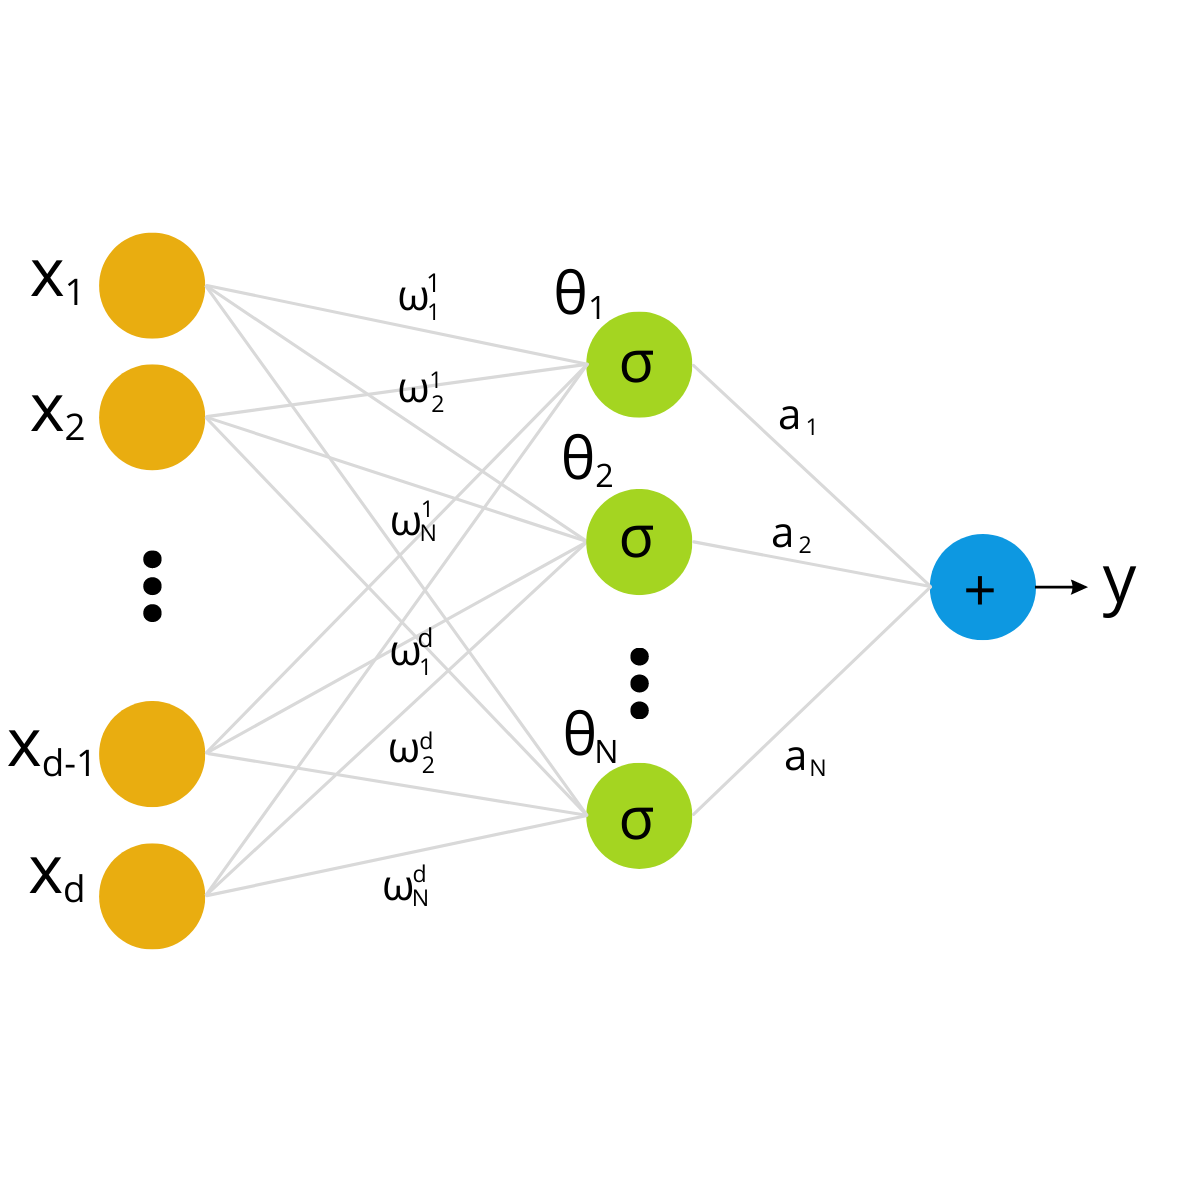
\includegraphics[scale=1.2]{img/MLP.png}
    \caption{Visualización de una red neuronal de una capa}
    \label{fig:MLP}
\end{figure}

% \subsubsection{Aspectos teóricos}
% \subsubsubsection{Teoremas de aproximación universal}
\subsubsection{Teoremas de aproximación universal}
La siguiente subsección está basada en el trabajo de Cybenko (1989) \cite{cybenko}. Para la demostración usaremos elementos de Análisis Funcional, como lo son el Teorema de Hahn-Banach y el Teorema de representación de Riesz. Por otro lado, una versión del mismo resultado demostrado en el mismo periodo por Hornik et al. usa el Teorema de Stone-Weirstrass \cite{hornik}.
\begin{definition}[Función sigmoide]
Decimos que una función $\sigma$ es sigmoide si cumple
$$ \sigma(t) = \begin{cases}
1 & \text{ cuando }t\to\infty \\
0 & \text{ cuando }t\to-\infty
\end{cases}$$
\end{definition}
\begin{example}[Función logística]
A la función $\sigma:\R\mapsto (0,1)$
$$ \sigma(t):= \displaystyle\frac{1}{1+e^{-t}}$$
se le llama función logística. Es el ejemplo más común de una función sigmoide continua.
\\ La activación de Heavisde es también una función sigmoide.
% observacion funcion softmax ???
\end{example}
Asumimos el siguiente resultado sin demostración. Está basado en el uso del teorema de convergencia dominada.
\begin{lemma}
\label{lemma:discrim}
Sea $\sigma$ una función sigmoide, medible y acotada, entonces cumple la siguiente propiedad:
$$ \int_{[0,1]^n}\sigma(y^Tx+\theta)d\mu(x)=0\espacio \forall y\in\R^n,\forall\theta \in\R\espacio \Longrightarrow \espacio  \mu\equiv 0$$
En particular esto es cierto para cualquier función sigmoide continua.
\end{lemma}
\begin{theorem}[Teorema de aproximación universal para activación sigmoide]
\label{teo:AU}
Sea $\sigma$ una función sigmoide continua. Entonces el conjunto de funciones de la forma
$$ G(x) = \displaystyle \sum^N_{j=1}a_j\sigma(w^T_jx+b_j)$$
es denso en $\mathcal{C}([0,1]^n)$, con $\b_j\in\R$, $a_j\in\R\espacio \forall j=1,\dots,N$ y $w_j\in\R^n\espacio\forall j=1,\dots,N$. Dicho de otro modo, para todo $f\in\mathcal{C}([0,1]^n)$ y $\epsilon>0$, $\exists G(x)$ de la forma anterior que cumple
$$ |G(x)-f(x)|<\epsilon\espacio\forall x\in [0,1]^n\,.$$
\end{theorem}
\begin{proof}
\gris
Sea $S\subset\mathcal{C}([0,1]^n)$ el conjunto de las funciones de la forma $\displaystyle \sum^N_{i=j}a_j\sigma(w^T_jx+b_j)$, con  $b_j\in\R$, $a_i\in\R\espacio \forall j=1,\dots,N$ y $w_j\in\R^n\espacio\forall j=1,\dots,N$, y notemos que es un subespacio lineal de $\mathcal{C}([0,1]^n)$. Veamos que $\bar S$ (la cerradura de $S$) es $\mathcal{C}([0,1]^n)$. Por contradicción, si asumimos lo contrario entonces $\bar S$ es un subespacio cerrado propio de $\mathcal{C}([0,1]^n)$. Luego por Hahn-Banach existe un funcional lineal $L$ en $\mathcal{C}([0,1]^n)$, no nulo, pero que se anula en $\bar S$ (y por ende en $S$).

\newp Por el teorema de representación de Riesz, el funcional $L$ debe ser de la forma
$$ L(h) = \displaystyle\int_{[0,1]^n}h(x)d\mu(x)$$
para $\mu$ medida en $[0,1]^n$ y $\forall h\in \mathcal{C}([0,1]^n)$. Luego en particular se cumple que
$$\int_{[0,1]^n}\sigma(y^Tx+\theta)d\mu(x)=0 \espacio \forall y\in\R^n,\forall\theta \in\R$$. Por lema \ref{lemma:discrim}, $\mu\equiv 0$, con lo cual el funcional lineal $L$ es nulo. Como esto es una contradicción, $\bar S = \mathcal{C}([0,1]^n)$, i.e., $S$ es denso en $\mathcal{C}([0,1]^n)$.\findem
\negro
\end{proof}
\begin{remark}
A las funciones que cumplen la propiedad del lema \ref{lemma:discrim} se les llama funciones discriminatorias. El resultado vale entonces para cualquier función discriminatoria continua. Además, se puede generalizar a funciones sigmoide medibles y funciones sigmoide arbitrarias agregando ciertas restricciones adicionales.

Más aún, existen variados resultados que proponen cotas para el tamaño de la red neuronal dependiendo de la función a aproximar. La versión del Teorema de Aproximación Universal que hemos visto corresponde al caso de ancho arbitrario, donde ancho se refiere a la cantidad de perceptrones de la capa. Análogamente existen versiones de ancho acotado y profundidad arbitraria, donde profundidad se refiere a la cantidad de capas.
\end{remark}
% \begin{remark}[Generalizaciones del Teorema \ref{teo:AU}]
% ...
% \end{remark}

El siguiente resultado nos muestra que el Teorema de aproximación universal nos sirve para implementar un clasificador basado en separaciones del espacio con una red de una sola capa. Primero sea $P_1,\dots,P_k$, $k\in\N$ una partición de $[0,1]^n$, definiremos una función de decisión como un $f:[0,1]^n\mapsto \{1,\dots,k\}$ que cumple
$$ f(x) = j \espacio \ssi \espacio x\in P_j \,.$$
\begin{theorem}
Sea $\sigma$ una función sigmoidal continua. Sea $f$ una función de decisión para alguna partición $\mu$-medible y finita, donde $\mu$ es la medida de Lebesgue en $[0,1]^n$. Para cualquier $\epsilon>0$ existe una suma finita de la forma
$$ G(x) = \displaystyle \sum^N_{j=1}a_j\sigma(w^T_jx+b_j) \,,$$
y un conjunto $D\subset [0,1]^n$ tal que $\mu(D)\geq 1-\epsilon$ y que cumple
$$ |G(x)-f(x)|<\epsilon\espacio \text{ para }x\in D \,.$$
\end{theorem}
\begin{proof}
\gris
Recordemos el Teorema de Lusin, que nos dice que una función finita $\mu$-c.s. es medible si y solo si es una función continua en casi todo su dominio. Luego existe una función continua $h$ y un conjunto $D$ tal que $\mu(D)\geq 1-\epsilon$ de modo que 
$$ h(x)=f(x) \espacio \forall x \in D \,.$$
Como $h$ es continua, por Teorema \ref{teo:AU}, existe una función $G$ de la forma $$G(x)=\displaystyle \sum^N_{i=j}a_j\sigma(w^T_jx+b_j)\,,$$
con  $b_j\in\R$, $a_i\in\R\espacio \forall j=1,\dots,N$ y $w_j\in\R^n\espacio\forall j=1,\dots,N$ que satisface
$$ |G(x)-h(x)|<\epsilon \espacio \forall x\in [0,1]^n\,.$$
Entonces para $x\in D$ tendremos $|G(x)-f(x)|<\epsilon$\,. \findem
\negro
\end{proof}

\subsubsection{Entrenamiento de una red neuronal con Gradiente Estocástico}
Consideremos el caso en el que tengamos una sucesión de $n$ puntos de datos $(x_1,y_1),\dots,(x_n,y_n)\subset \R^d\times\R$. Sea además, $l:\R\times\R\mapsto\R$ una función de error, y denotemos:
$$ \mathcal{L}(\theta) = \displaystyle\frac{1}{N}\sum_{i=1}^n l(y_i,\hat y_i(x_i,\theta)) \,.$$ 
Usaremos el Algoritmo de Descenso de Gradiente Estocástico para minimizar esta función de pérdida. Sin embargo notemos que esto no es tarea fácil, pues involucra el cómputo del gradiente de $\mathcal{L}$, considerando que la dimensionalidad de $\theta$ corresponde al número de parámetros totales de la red neuronal (potencialmente muy grande). Estudiemos como se realiza esto en la práctica.
% \subsubsubsection{Funciones de error}
\subsubsubsection{Cálculo de gradiente con \textit{Back-propagation}}
% \subsubsubsection{Tensores}
Back-Propagation es un algoritmo para calcular derivadas en contextos generales, aunque es principalmente usada en el contexto de redes neuronales. Es particularmente útil cuando tenemos cálculos sucesivos, lo cual es el caso de las redes neuronales, más aún si constan de varias capas de profundidad. Veamos un ejemplo para inspirar su uso.

\newp Sean $\theta$ el conjunto de parámetros de una red neuronal que queremos ajustar. Sabemos que para Gradiente Estocástico tendremos que saber computar el gradiente en un punto para cualquier parámetro en $\theta$. Consideremos una pérdida cuadrática y una aproximación de un dato $y_i$ de la forma
$$ \hat y_i = \displaystyle \sum^N_{j=1} a_j\sigma(\omega^T_j x_i+b_j) $$
Tratemos de calcular la derivada de $l_i=(y_i-\hat y_i)^2$ con respecto a $a_k$, con $k\in\{1,\dots,N\}$:
$$ \frac{\partial l_i}{\partial a_k} = \frac{\partial (y_i-\hat y_i)^2}{\partial a_k} = 2(y_i-\hat y_i) \frac{\partial (y_i-\hat y_i)}{\partial a_k} \,.$$
Notemos que hasta este punto, sólo usamos la regla de la cadena. Ahora como $y_i$ es un punto fijo de dato que no depende de $a_k$, nos queda:
$$ \frac{\partial l_i}{\partial a_k} = 2(y_i-\hat y_i) \frac{\partial (y_i-\hat y_i)}{\partial a_k} =  -2(y_i-\hat y_i) \frac{\partial\hat y_i}{\partial a_k} =  -2(y_i-\hat y_i) \frac{\partial[\sum^N_{j=1} a_j\sigma(\omega^T_j x_i+b_j)]}{\partial a_k} = -2(y_i-\hat y_i)\sigma(\omega_k^Tx_i+b_k)$$
Denotaremos ahora las variables auxiliares siguientes. El objetivo será simplificar lo anterior:
\begin{itemize}
    % \item $l_i = l(y_i,\hat y_i)$
    \item $z_i = (y_i-\hat y_i)$
    \item $u^j_i = a_j\sigma(\omega^T_j x_i+b_j)$
    \item $v^j_i = \omega^T_j x_i+b_j$
\end{itemize}
Podemos reescribir el cálculo de la última linea usando las variables auxiliares:
$$ \frac{\partial l_i}{\partial a_k} = 2(y_i-\hat y_i) \frac{\partial[\sum^N_{j=1} a_j\sigma(\omega^T_j x_i+b_j)]}{\partial a_k} = 2z_i \frac{\partial[\sum^N_{j=1} u^j_i]}{\partial a_k} = 2z_i \frac{\partial u_i^k}{\partial a_k} \,.$$
En este punto podemos notar que 
$$ \frac{\partial u_i^k}{\partial a_k} = \frac{\partial[a_k \sigma(v_i^j)]}{\partial a_k} = \sigma(v_i^j) \espacio \therefore \espacio \frac{\partial l_i}{\partial a_k}=2z_i \sigma(v_i^j)$$
Si bien agregar las variables auxiliares nos hace pesada la notación, la idea es guardar la información paso por paso a medida que los valores ``avanzan'' en la red neuronal hasta llegar a la predicción. Esto a la larga será útil, pues se nos facilitan los cálculos, como vimos en derivar $\frac{\partial l_i}{\partial a_k}$. Por otro lado notemos que podemos llegar a $l_i$ de manera acumulativa desde los parámetros usando las variables auxiliares.
\begin{itemize}
    \item $l_i = z_i^2$
    \item $z_i = (y_i-\sum^N_{j=1}u_i^j)$
    \item $u^j_i = a_j\sigma(v_i^j)$
    \item $v_i^j = \omega^T_j x_i+b_j$
\end{itemize}
Luego usando la regla de la cadena podemos deducir que
$$ \frac{\partial l_i}{\partial a_k} = \frac{\partial l_i}{\partial z_i}\frac{\partial z_i}{\partial u_i^j}\frac{\partial u_i^j}{\partial a_k} = 2z_i \cdot 1 \cdot \sigma(v_i^j) \,$$
i.e., hicimos el mismo cálculo anterior pero basado en cálculos simples de derivadas usando las variables auxiliares. Veamos otro ejemplo. Calcularemos $\frac{\partial l_i}{\partial b_k}$ usando este principio:
$$ \frac{\partial l_i}{\partial b_k} = \frac{\partial l_i}{\partial z_i}\frac{\partial z_i}{\partial u_i^j}\frac{\partial u_i^j}{\partial v_i^j}\frac{\partial v_i^j}{\partial b_k} = 2z_i \cdot 1 \cdot a_k\sigma'(v_i^j)\cdot 1 = 2 (y_i-\sum^N_{j=1}u_i^j)a_k\sigma'(\omega^T_j x_i+b_j) \,$$
donde $\sigma'$ es la derivada de la función de activación $\sigma$ (unidimensional). \newp Notemos la facilidad con la que llegamos a la expresión final, y más aún, notemos que muchas de las derivadas parciales que usamos también se usaron para computar $\frac{\partial l_i}{\partial a_k}$. Se puede hacer un cálculo análogo para llegar a $\frac{\partial l_i}{\partial \omega_k}$, con lo cual tendríamos calculado el gradiente de $l_i$. 
\newp El algoritmo Back-Propagation consiste en el uso exhaustivo de la \textbf{regla de la cadena}. Calculamos derivadas parciales paso por paso y las guardamos para usarlas en cada parámetro. De este modo que sólo computaremos derivadas simples y guardarlos evitará hacer cálculos redundantes. %La única restricción que tenemos para usar Back-Propagation es que no hayan cálculos circulares.
En nuestro caso no era imposible calcular el gradiente, pero a medida que las redes neuronales sean más profundas, más profundas serán las dependencias entre variables y por ende más cálculos se ahorrarán si usamos regla de la cadena, además de simplificar el computo.

\newp Las bibliotecas que implementan redes neuronales, como \textit{pytorch} implementan este algoritmo implícitamente, de modo que al definir las operaciones entre variables, se guardan las derivadas parciales respectivas. Durante el entrenamiento, una vez que la información pasa a través de la red neuronal para computar una predicción, se computará un error (\textit{forward}). Enseguida, se computa el gradiente usando las operaciones que estaban guardadas, haciendo fluir la información en reversa hasta tener el valor de cada derivada parcial (\textit{backward}). Esto nos da una manera eficiente de usar descenso de gradiente estocástico.

\subsubsubsection{Problemas y prácticas usuales}
% El uso de redes neuronales ha ido evolucionando con el tiempo. Muchas de las innovaciones son resultado de experimentos que han funcionado bien en la práctica.
Hasta ahora hemos observado las capacidades teóricas de las redes neuronales de una sola capa. Si bien poder aproximar funciones continuas parece una capacidad muy valiosa, no siempre estaremos intentando aproximar funciones con buenas propiedades. Es más, muchas veces no tendremos ninguna garantía de que las funciones que estamos tratando de aproximar existan. Tener un cierto grado de profundidad nos ayuda a aumentar el poder de expresividad de los valores de salida. A su vez podremos disminuir el número de perceptrones en cada capa.
% figura
\newp Lamentablemente, un problema que se encuentra al entrenar redes neuronales profundas es el \textbf{desvanecimiento del gradiente}. Esto sucede cuando el valor de las derivadas parciales es pequeño, evitando que puedan actualizarse valores de capas iniciales usando descenso de gradiente. Dentro de las soluciones que se han explorado para evitar este problema está el uso de la función de activación \textit{ReLU} (\textit{rectified linear unit}), que está dada por:
$$ ReLU(t) = \begin{cases}
t & \text{ cuando }t\geq0 \\
0 & \text{ cuando }t<0
\end{cases}$$
Si bien esta función no es sigmoide y es no-acotada, es mucho más fácil de computar y es invariante a la escala. El problema de que no sea derivable en $0$ se arregla simplemente asignando $1$ o $0$ como valor de la derivada en aquel punto. Por último notar que podemos lograr funciones que si son sigmoides al acoplar dos funciones \textit{ReLU} o más. Un ejemplo de esto es la función $\sigma$ siguiente:
$$ \sigma(t) = \frac{1}{2}(ReLU(t+1)-1-(ReLU(t-1)-1))\,,$$
que es una función sigmoide continua, y por ende cumple con las hipótesis del Teorema \ref{teo:AU}. En la figura \ref{fig:fun_activ} se muestran algunas de las funciones de activación que se han mencionado en esta subsección.
\begin{images}[\label{fig:fun_activ}]{Ejemplos de funciones de activación}
	\addimage{RRNN_escalon}{width=6.5cm}{Activación de Heaviside}
	\addimage{RRNN_logistic}{width=6.5cm}{Logística}
	\imagesnewline
	\addimage{RRNN_ReLU}{width=6.5cm}{$ReLU(t)$}
	\addimage{RRNN_two_ReLUs}{width=6.5cm}{$\frac{1}{2}(ReLU(t+1)-1-(ReLU(t-1)-1))$}
\end{images}


% \subsubsection{Otros tipos de redes neuronales}
% \subsubsubsection{Redes convolucionales}
% \subsubsubsection{Redes recurrentes}

% \subsubsection{Aplicaciones en matemáticas}


\newpage
\section{Movimiento Browniano y difusiones}
\label{browniano}
% \documentclass[../main/main.tex]{subfiles}
% \begin{document}
% \chapter{Movimiento, Browniano Procesos de difusión y Aplicaciones}

\subsection{Movimiento Browniano}
% clase 19 ajustar


% corregir redacción
Se busca definir una función real de al variable $t \in \mathbb{R}_{+}$ (interpretada como tiempo), que sea continua y que sea \textit{} forma de darle sentido a lo anterior es mediante un \textbf{paseo aleatorio}: sean 
\begin{itemize}
\item $X_1, X_2, X_3, \ldots $ variables aleatorias independientes e idénticamente distribuidas tales que 
    \begin{equation*}
            \P(X_{i} = -1) = \P(X_i = 1) = \frac{1}{2}\,.
    \end{equation*}
 \item $\forall  n \in \N$,
     \begin{equation*}
             S_n := \sum_{i=1}^{n} X_i, ~ ~ ~ \text{ con } S_0 = 0\,.
     \end{equation*}
 \item $\forall t\in \mathbb{R}_{+}$, $S_t$ es la interpolación lineal de la colección $(S_{n})_{n \in \N}$.
\end{itemize}

%Para $t$ lo suficientemente grande y escalando tiempo y espacio adecuadamente, gráfico de $S_t$ pasa a ser análogo al de la figura (\ref{fig:c6_1}).
% corregir redacción
Específicamente, el escalamiento es: $\forall a >0$, definimos:
\begin{equation*}
    B_t^{(a)} = \sqrt{\frac{t}{n}}   S_n = \sqrt{t}
    \underbrace{\frac{1}{\sqrt{n} } \sum_{i=1}^{n} X_i}_{\substack{\text{aprox. } \mathcal{N}(0,1) \\ \text{ por TCL.}}}\,.
\end{equation*}

con lo que se tiene que $B_t^{(a)} \approx \mathcal{N}(0,t)$. También es directo ver que para $m > n$ enteros, $S_m - S_n$ es independiente de $S_n$, es decir, $(S_n)_{n \in \N}$ tiene \textbf{incrementos independientes}, lo cual se manifiesta también en $(B_{t}^{(a)})_{t \geq 0}$. Esto motiva:

\begin{definition}[Movimiento Browniano]
        \label{def:mb}
        Un movimiento browniano es un proceso estocástico (es decir, una colección de variables aleatorias indexadas por $t \geq 0$) denotado $(B_t)_{T \geq 0}$, que satisface:     
\renewcommand{\labelenumi}{\roman{enumi})}
\begin{enumerate}
    \item $B_0 = 0$ casi seguramente.
    \item Tiene \textbf{incrementos independientes}: $\forall  t\geq 0$,
        \begin{equation*}
                (B_{t+s} - B_t)_{s \geq 0}, \text{ es independiente de } (B_{s})_{0 \leq s \leq t}\,.
        \end{equation*}
    \item Tiene \textbf{incrementos normales}:\espacio $\forall  t,s \geq 0$,
        \begin{equation*}
                B_{t+s} - B_t \sim \mathcal{N}(0,s)\,.
        \end{equation*}
    \item Es un proceso \textbf{continuo}: con probabilidad $1$, la función $t \mapsto B_t$ es continua en $t$.
\end{enumerate}
\end{definition}

La ley del proceso $(B_{t}^{(a)})_{t \geq 0}$ converge, cuando $a \rightarrow \infty$, a la ley del movimiento browniano $(B_t)_{t \geq 0}$, en un sentido adecuado (esto se llama \textit{teorema de Donsker}). Por otra parte, $(B_t)_{t \geq 0}$ también se conoce como \textbf{Proceso de Wiener}. El nombre \textit{browniano} proviene del botánico Robert Brown, quien observó el movimiento errático de partículas de polen en el agua. Posteriormente, Einstein explicó este movimiento como resultado de muchas pequeñas colisiones del polen con las moléculas de agua circundantes.
\newp Dado lo anterior surge la pregunta: ¿ Existe un proceso cumpliendo las condiciones de la definición anterior?

\begin{theorem}
    \label{teo:mb}
    El movimiento browniano existe.
\end{theorem}
La demostración queda pendiente. Por ahora veamos algunas propiedades básicas del movimiento browniano.

\begin{proposition}
$\forall ~ 0 = t_0 < t_1 < \ldots < t_n$ , la colección 
\begin{equation*}
    \left( \frac{B_{t_i} - B_{t_{i-1}}}{\sqrt{t_i - t_{i-1}} }
    \right)_{i = 1, \ldots,n} \text{ es i.i.d } \sim \mathcal{N}(0,1)\,.
\end{equation*}
\end{proposition}
\begin{proof}
\gris
Directa de la definición.
\negro
\end{proof}

Esto da lugar a un método sencillo para generar un movimiento browniano discretizado: para un horizonte $T > 0$ y $n \in \N$, sea $\Delta t = \frac{T}{n}$, y $t_i = i \Delta t$.  Dadas $Z_1, \ldots, Z_n$ i.i.d. $\mathcal{N}(0,1)$, entonces el proceso $(Y_{t})_{t \in [0,T]}$: 
\begin{equation*}
    Y_{t_i} := \sqrt{\Delta t} \sum_{j=1}^{i} Z_j
\end{equation*}
interpolado linealmente entre $t_i$'s, es una aproximación de $(B_t)_{t \in [0,T]}$ (de hecho, tiene exactamente la misma ley en la malla $0 = t_0 < t_1 < \ldots < t_n = T$). 

\begin{proposition}
Se tienen las siguientes proposiciones:
\begin{enumerate}
    \item \label{prop1:a} $\forall  t_0 > 0$, el proceso $X_t := B_{t + t_0} - B_{t_0}$ es un movimiento browniano.
    \item \label{prop1:b} $\forall c > 1$, el proceso $X_t := \frac{1}{\sqrt{c}} B_{ct}$ es un movimiento browniano.
    \item \label{prop1:c} El proceso $X_t := B_1 - B_{1-t}$ es un movimiento browniano en $[0,1]$.
    \item \label{prop1:d} El proceso $X_t := t B_{\frac{1}{t}}$ es un movimiento browniano. ($X_0 = 0$)
    \item \label{prop1:e} El proceso $X_t := -B_{t}$ es un movimiento browniano.
\end{enumerate}
\end{proposition}

\begin{proof}
\gris
Probemos \ref{prop1:b}, el resto queda propuesto como \ejercicio \gris. Debemos probar que $X_t = \frac{1}{\sqrt{c}} B_{ct}$ cumple con las condiciones de la definición (\ref{def:mb}). Es claro  que las condiciones I,II y IV son directas del hecho que $(B_t)_{t \geq 0}$ es un movimiento browniano. Además: 
\begin{equation*}
    X_{t+s} - X_t = \underbrace{\frac{1}{\sqrt{c} } \left( B_{ct + cs} - B_{ct} \right)}_{\mathcal{N}(0,cs)} \sim  \mathcal{N}(0,s)\,.
\end{equation*}
\findem
\negro
\end{proof}

A pesar de que son continuas, las \textbf{trayectorias} de un movimiento browniano son bastante irregulares. La trayectoria de un movimiento browniano es la función aleatoria:
\begin{equation*}
     t \mapsto B_t
\end{equation*}

\begin{theorem}
$$\P( \exists t \geq 0 \text{ tal que } B_t \text{ es derivable en } t) = 0 \,.$$
\end{theorem}

La demostración de dicho teorema escapa a los contenidos del curso. 

\newp El comportamiento de las \textbf{oscilaciones} del movimiento browniano cerca de $t=0$ y $t=\infty$ queda descrito por el siguiente resultado:

\begin{theorem}[Ley del Logaritmo Iterado]
$\P$- casi seguramente se cumple:
% \renewcommand{\labelenumi}{\roman{enumi})}
\begin{enumerate}
     \item \label{lli:1} $\limsup_{t \searrow 0} \frac{B_t}{\sqrt{ 2t \log \log {1/t}}} = 1$
     \item \label{lli:2} $\liminf_{t \searrow 0} \frac{B_t}{\sqrt{ 2t \log \log {1/t}}} = -1$
     \item \label{lli:3} $\limsup_{t \rightarrow \infty} \frac{B_t}{\sqrt{ 2t \log \log {t}}} = 1$
     \item \label{lli:4} $\liminf_{t \rightarrow \infty} \frac{B_t}{\sqrt{ 2t \log \log {t}}} = -1$
\end{enumerate}
\end{theorem}

\newp La demostración de este resultado utiliza herramientas fuera del alcance del curso. Gráficamente  \ref{lli:1} y \ref{lli:2} significa que la trayectoria de $(B_{t})_{t \geq 0}$ cruza o pasa cerca del gráfico de la función $f(t) = \sqrt{2t \log \log (t)} $ infinitas veces cuando $t \rightarrow \infty$, y lo mismo para $-f(t)$. 

\begin{proposition}
     $$\operatorname{Cov}(B_t,B_s) = t \wedge s := \min(t,s)\,.$$ 
\end{proposition}
\begin{proof}
\gris
 Para $0 \leq s \leq t$ tenemos: 
\begin{align*}
     \operatorname{cov}(B_t, B_s)
     &= \E (B_t B_s) - \underbrace{(\E (B_t))(\E (B_s))}_{= 0} \\
     &= \E \underbrace{((B_t - B_s)B_s)}_{\text{indep.}} + \E(B_s) \\
     &= \underbrace{\left( \E(B_t - B_s) \right)}_{=0} + \underbrace{\var({Bs})}_{s}\\
     &= s = s \wedge t
\end{align*}
\findem
\negro
\end{proof}

\subsection{Martingalas}
Para definir lo que es una martingala y otros conceptos relacionados se requiere del siguiente concepto:
% def repetida
\begin{definition}[Filtración]
Dado un espacio de probabilidad $(\Omega, \mathcal{F}, \P)$, una \textbf{filtración} es una colección $\mathbb{F} = (\mathcal{F}_{t})_{t \geq 0}$ de sub $\sigma$-álgebras de $\mathcal{F}$ que es \textbf{creciente}, es decir, $\mathcal{F}_t \subseteq \mathcal{F}_s$, $\forall s \leq s$.
\end{definition}

$\mathcal{F}_t$ representa la \textbf{información} disponible en momento $t$, es decir, la colección de eventos de $\mathcal{F}$ que pueden definirse a partid e la información hasta $t$. 

\newp Dado un proceso estocástico $(X_t)_{t \geq 0}$, definimos su \textbf{filtración natural} como 
\begin{equation*}
        \mathcal{F}^{X}_t := \sigma\left( \{ X_s : s \leq t \}\right) 
\end{equation*}

\newp Decimos que un proceso $(X_{t})_{t \geq 0}$ es \textbf{adaptado} a una filtración $(\mathcal{F}_t)_{t \geq 0}$ 
si $X_t$ es $\mathcal{F}_t$ medible $\forall t$. En general se asume que los procesos con los que se trabaja son adaptados. Evidentemente, $(X_t)_{t \geq 0}$ es $(\mathcal{F}^X_t)_{t \geq 0}$ - adaptado.

\newp Cuando trabajamos con un proceso (por ejemplo un movimiento browniano y no se menciona la filtración, esta implícito que se usa la filtración natural. 

\newp Para comprender el concepto de martingala es provechoso reflexionar sobre el siguiente ejemplo: si $X_t$ representa la riqueza de una persona en el instante $t$, la cual evoluciona de acuerdo a reglas aleatorias de un cierto \textit{juego} (ejemplo: apuestas, fluctuaciones de la bolsa), entendemos que el juego es \textbf{justo} si la riqueza futura no crece ni decrece, en esperanza.
% def repetida
\begin{definition}[Martingala]
Dado un espacio de probabilidad $(\Omega, \mathcal{F}, \P)$ con filtración $\mathbb{F} = (\mathcal{F}_{t})_{t \geq 0}$, una \textbf{martingala} es un proceso $(X_t)_{t \geq 0}$ adaptado tal que:
\begin{itemize}
    \item $\forall  t \geq 0$, $X_t \in L^{1}$, es decir, $\E \abs{X_t} < \infty$.
    \item $\forall s \leq t$, 
            \begin{equation*}
                    \E \left( X_t \mid \mathcal{F}_s \right)  = X_s, \espacio \text{casi seguramente}\,.
            \end{equation*}
\end{itemize}
\end{definition}

Notemos que entonces $\E(X_t) = \E(X_0)$ que es constante para todo $t$. 

\iffalse  % esto ya se repasó en la sub-unidad dedicada a esperanzas condicionales
\newp El concepto de martingala está 
íntimamente relacionado con el calculo de esperanzas condicionales. A continuación se revisan algunas 
de las propiedades  necesarias en cuanto a este último concepto. 

\newp Si $X$ es una variable aleatoria y $\mathcal{G}$ es una sub $\sigma$ - álgebra, $Y = \E(X \mid \mathcal{G})$ 
es la única (casi seguramente) variable aleatoria $\mathcal{G}$-medible tal que 
\begin{equation*}
\E \left( \mathbbm{1}_{A} X  \right)  = \E\left( \mathbbm{1}_{A} T \right) , ~ ~ ~\forall  A \in \mathcal{G}
\end{equation*}

\begin{itemize}
        \item Si $X$ es $\mathcal{G}$- medible, entonces $\E(E \mid \mathcal{G} ) = X$ casi seguramente.
        \item Si $X \indep \mathcal{G}$, entonces $\E(X \mid \mathcal{G}) =
                \E (X)$, es decir, es constante casi seguramente.
        \item Si $Z$ es $\mathcal{G}$ - medible, entonces $\E(ZX \mid G) = Z\E(X \mid \mathcal{G})$ casi 
                seguramente.
\end{itemize}
\fi

\newp Cuando hay una filtración subyacente, se hace necesario re-definir el concepto de movimiento browniano:

\begin{definition}[Movimiento Browniano para un espacio filtrado]
Dado un espacio de probabilidad filtrado $(\Omega, \mathcal{F}, (\mathcal{F}_t)_{t \geq 0}, \P)$, un \textbf{movimiento browniano} es un proceso $(B_t)_{t\geq 0}$ adaptado que satisface:
\renewcommand{\labelenumi}{\roman{enumi})}
\begin{enumerate}
        \item   $B_0 = 0$, casi seguramente. 
        \item $\forall t \geq 0$, $(B_{t+s} - B_t)_{s \geq 0} \indep \mathcal{F}_t$. 
        \item $B_{t+s} - B_t \sim  \mathcal{N}(0,s)$, $\forall t,s \geq 0$. 
        \item Posee trayectorias continuas. 
\end{enumerate}
\end{definition}

Si no se especifica la filtración, se asuma la filtración natural (es decir, la definición original). 

\begin{proposition}
Dado $(\Omega, \mathcal{F},(\mathcal{F}_{t})_{t \geq 0}, \P)$ y un movimiento browniano 
$(B_{t})_{t \geq 0}$, entonces:

\begin{enumerate}
        \item \label{mba:1} $ (B_t)_{t \geq 0}$ es una martingala.
        \item \label{mba:2} $\left( B_t^2 - t \right)_{t \geq 0} $ es una martingala.
        \item \label{mba:3} $\exp\left( \sigma B_t - \frac{\sigma^2}{2}t \right) $ es una martingala
                , $\forall  \sigma >0$. 
\end{enumerate}
\end{proposition}

\begin{proof}
\gris
Comenzamos por \ref{mba:1}: 
\begin{align*}
    \E(B_t \mid \mathcal{F}_s ) &= \E (B_t - B_s \mid \mathcal{F}_s)
        + \E(B_s \mid \mathcal{F}_s) \\
        &= \E(B_t - B_s) + B_s \\ 
        &= B_s \,.
\end{align*}
Por otra parte, para \ref{mba:2}: 
\begin{align*}
\E(B_t^2 \mid \mathcal{F}_s) 
&=  \E \left( (B_{t} - B_{s}) \mid \mathcal{F}_s \right) + \E(B_s \mid
\mathcal{F}_s) - 2 \E \left( (B_t - B_s)B_s \mid \mathcal{F}_s \right) \\ 
&= \E\left( (B_t - B_s)^2 \right) + B_s^2 -2 \E \left((B_t - B_s) \mid \mathcal{F}_s\right)\\
&= t - s + B_s^2\,.
\end{align*}
Finalmente para \ref{mba:3}, recordemos que si $X \sim \mathcal{N}(\mu, \tau^2)$, entonces 
\begin{equation*}
        \E (e^{\lambda X}) = \exp\{\lambda \mu + \frac{\lambda^2 \tau^2}{2}\}\,.
\end{equation*}
Con esto 
\begin{align*}
        \E \left( e^{\sigma B_t} \mid \mathcal{F}_s \right) 
        &= \E \left( e^{\sigma (B_t - B_s)} e^{\sigma \B_s} \mid \mathcal{F}_s\right) \\
        &= e^{\sigma B_s} \E \left(e^{\sigma(B_t - B_s)} \mid \mathcal{F}_s\right) \\ 
        &= e^{\sigma B_s} \E \left( e^{\sigma(B_t - B_s)} \right) \\ 
        &= e^{\sigma B_s} e^{\sigma^2(t-s)/2}\,.
\end{align*}
\findem
\negro
\end{proof}

\subsection{Tiempos de Parada}
Buscamos definir tiempo aleatorios que \textbf{no utilicen información futura}, solamente lo que a ocurrido hasta el momento.
% def repetida
\begin{definition}[Tiempo de parada]
Dado un espacio de probabilidad filtrado $(\Omega, \mathcal{F}, (\mathcal{F}_t)_{t \geq 0}, \P)$, un \textbf{tiempo de parada} es una variable aleatoria $T \in [0, \infty]$ tal que 
\begin{equation*}
    \{ T \leq t \} \in \mathcal{F}_t, ~ ~ ~ \forall  t \,.
\end{equation*}
\end{definition}

\begin{example}
Para ilustrar la definición anterior, se estudian los siguientes ejemplos:
\begin{itemize}
    \item  Si se define $T_b := \inf \{t\geq 0 : B_t =
            b \}$ como \textit{la primera vez que} $B$ \textit{llega a} $b$, se tiene entonces que $T_b$ es un tiempo de parada. 
    \item Si se define $S_0 := \{ t \in [0,1]: B_t = 0 \}$ como \textit{la última vez antes de} $t=1$ \textit{que} $B$ \textit{toca a} $0$. 
            Entonces $S_0$ no es tiempo de parada. 
\end{itemize}
\end{example}
\begin{proof}
\gris
Veamos que $T_b$ es un tiempo de parada:
\begin{align*}
    \{ T_b \leq t \} 
    &= \{\exists s \in [0,1]: B_s = b \} \\
    &= \{\forall n \in \N, \exists r \in [0,1] \cap \mathbb{Q}, \abs{B_r -v} \leq \frac{1}{n}\}\\
    &= \bigcap_{n \in \N} \bigcup_{r \in [0,1] \cap \mathbb{Q}} \{
            \abs{B_r -b} \leq \frac{1}{n} \} \in \mathcal{F}_{t} \,.
\end{align*}
Lo que comprueba dicha afirmación. \findem
\negro
\end{proof}

\newp Surge la pregunta, cuando $(X_t)_{t \geq 0}$ es una martingala (es decir, un juego justo). Si uno detiene 
el juego en un tiempo aleatorio con la información disponible hasta el momento,
¿será posible obtener un beneficio de aquello? 

\newp Bajo cierta condición en el tiempo de parada, la respuesta será \textbf{no}. Para especificar lo anterior, 
necesitamos definir la $\sigma$-álgebra correspondiente a la información disponible hasta cierto 
tiempo de parada. 
\begin{definition}
Dado $(\Omega, \mathcal{F}, (\mathcal{F}_t)_{t \geq 0}, \P)$ y un tiempo de parada $T$, la 
$\sigma$-álgebra asociada a $T$ es:
\begin{equation*}
        \mathcal{F}_T := \{ A \in \mathcal{F}: \forall t \geq 0, ~ A \cap
        \{T\leq t\} \in \mathcal{F}_t \}
\end{equation*}
\end{definition}
\ejercicio  \gris : Probar que $\mathcal{F}_T$ es $\sigma$-álgebra. \negro

\begin{theorem}[Muestreo opcional de Doob]
Dados $(\Omega, \mathcal{F}, (\mathcal{F}_t)_{t \geq 0}, \P)$ y una martingala $(X_t)_{t \geq 0}$, 
sean $T$, $S$ tiempos de parada tales que $S \leq T \le K$ con $K>0$ una constante. Entonces 
\begin{equation*}
        \E \left[ X_t \mid  \mathcal{F}_s \right]  = X_s,  ~ ~ ~ \text{c.s.}\,.
\end{equation*}
\end{theorem}
La demostración de este teorema utiliza herramientas fuera del alcance del curso. 

\newp El resultado anterior es útil para algunos cálculos sobre tiempos de parada. La condición de $T$ acotado suele ser demasiado restrictiva. Para $T$ tiempo de parada no acotado, se trabaja con $T \wedge n$ y luego se hace $n \to \infty$. Esta técnica se denomina \textbf{localización}. Veamos un ejemplo:

\begin{proposition}
Para $a \in \mathbb{R}$, sea $T_a = \inf \{ t \ge 0: B_t = a \}$. Entonces $T_a < \infty$ casi seguramente y su ley viene dada por su transformada de Laplace.
\begin{equation*}
        \E \left( e^{-\lambda T_{a}} \right)  = e^{-\sqrt{2\lambda} \abs{a} }\,,
\end{equation*}
o equivalente, su densidad es 
\begin{equation*}
        f_{T_{a}} = \frac{\abs{a}}{\sqrt{ 2 \pi x^3}} \exp({{-a^2}/{2x}}), ~ ~ ~ \forall x > 0\,.
\end{equation*}
\end{proposition}
\begin{proof}
\gris
Sea $a>0$. Sea además la martingala $X_t = \exp(\sigma B_t - \frac{\sigma^2}{2}t)$ y usemos el teorema al tiempo de parada acotado $T_a \wedge n$, para $n \in \N$. Luego $\E (X_{T_a \wedge n}) = \E(X_0) = 1$. Queremos  hacer $n \to \infty$. Notemos que:
\begin{itemize}
\item $X_{T_{a} \wedge n} = \exp\left(\sigma B_{T_{a} \wedge n} - \frac{\sigma^{2}}{2} 
        T_a \wedge n \right)  \le e^{\sigma a}$, es decir, la sucesión $(X_{T_a \wedge n})_{n \in \N}$ está dominada por $e^{\sigma a}$.
\item En $\{T_a < \infty \}$, $X_{T_a \wedge n} \xrightarrow[n]{} X_{T_a}$
\item En $\{T_a = \infty \}$, $X_{T_a \wedge n} = X_n = \exp\left( \sigma B_n - \frac{\sigma^2 n}{2} \right)  \xrightarrow[n]{} 0$.  % n\to\infty % ????
\end{itemize}
Luego, usando el teorema de convergencia dominada: 
\begin{align*}
    1 &= \lim_n \E(X_{T_{a} \wedge n}) \\ 
    &\stackrel{\text{TCD}}{=} \E\left(\lim_n X_{T_a \wedge n} \right)\\
    &= \E \left( \lim_n \mathbbm{1}_{\{T_a < \infty\}} X_{T_a \wedge n} + 
    \lim_n \mathbbm{1}_{\{T_{a} = \infty\}} X_{T_a \wedge n} \right)\\
    &= \E \left( \mathbbm{1}_{\{ T_a < \infty \}}  X_{T_a}  \right)  = \E \left( \mathbbm{1}_{\{T_a < \infty \}} \exp( \sigma B_{T_a} - \frac{\sigma^2 T_a}{2}) \right)\,.
\end{align*}
Es decir, 
\begin{equation*}
    \E \left[ \mathbbm{1}_{\{T_a < \infty \}} \exp(-\sigma^2 T_a / 2) \right] = e^{-\sigma a}
\end{equation*}
Haciendo $\sigma \to 0$, se obtiene $\P(T_a < \infty) = 1$. Tomando $\sigma = \sqrt{2\lambda}$, se llega a lo deseado. El caso $a < 0$ se deduce directamente pues $-B_t$ es también un movimiento browniano.\findem
\negro
\end{proof}

\newp La siguiente desigualdad también es útil:
\begin{theorem}[Desigualdad de Doob]
Si $(X_t)_{t \in [0,T]}$ es una martingala continua, entonces 
\begin{equation*}
    \E \left[ \sup_{0 \le  t \le  T} \abs{X_t}^2 \right] \le 4 \E \left[ \abs{X_T}^2 \right]\,.
\end{equation*}
\end{theorem}

\subsection{Integral Estocástica y Cálculo de It\^{o}}
Como motivación consideremos $(X_t)_{t \ge 0}$ un proceso con trayectorias continuas y derivables. Se puede definir la \textbf{integral} de $f$ con respecto a $X$ como
\begin{equation*}
        \int_{0}^{t} f(s) dX_s := \int_{0}^{t} f(s) \frac{dX_s}{ds} ds \,.
\end{equation*}

Lamentablemente, no podemos hacer los mismo con un movimiento browniano $(B_t)_{t \ge 0}$, pues $\displaystyle\frac{dB_t}{dt}$ \textbf{no existe}. Luego, si queremos definir 
\begin{equation*}
        \int_{0}^{t} f(s) dB_s
\end{equation*}
tendremos que seguir un enfoque distinto. Integrales de este tipo son muy útiles; por ejemplo, para definir ecuaciones diferenciales estocásticas. 
\newp Permitiremos que el integrando $f(s)$ también sea un proceso, i.e., definiremos 
$$\int_{0}^{t} X_s dB_s \,.$$ 

\subsubsection{Construcción}
Sea $(\Omega, \mathcal{F}, (\mathcal{F}_t)_{t \geq 0}, \P)$ un espacio filtrado, sea $(B_t)_t{t \ge 0}$ un movimiento browniano con respecto a este espacio. En primer lugar, definiremos la integral con respecto a $B$ para una cierta clase de procesos, llamados \textbf{procesos simples predecibles}:
\begin{definition}[Proceso Simple Predecible]
Un proceso $(H_t)_{0 \le  t \le T}$ se dice simple predecible si se escribe de la forma 
\begin{equation*}
    H_t = \sum_{i=1}^{k} A_i \mathbbm{1}_{\{ t_{i-1}, t_i \}} (t)\,.
\end{equation*}
para ciertos instantes $0 = t_0 < t_1 < \ldots, t_k = T$, $(A_i)_{i=1}^{k}$ son variables aleatorias $\mathcal{F}_{t_{i -1}}$ - medibles, y tales que $H$ cumple $\E(\int_{0}^{T} H_s^{2} ds) < \infty$.
\end{definition}

\begin{definition}[Integral Estocástica]
Dado un tal $H$, la \textbf{integral estocástica} de $H$ con respecto a $B$ es el proceso $\left(I(H)_t \right)_{t \in [0,T]}$. Definido como 
\begin{equation*}
    I(H)_t = \sum_{i=1}^{k} A_i \left( B_{t_i \wedge n} - B_{t_{i-1} \wedge t} \right) =: \int_{0}^{t} H_s dB_s\,.
\end{equation*}
Es decir, para $t \in (t_j, t_{j+1}]$ 
\begin{equation*}
    I(H)_t = \sum_{i=1}^{j} A_i\left( B_{t_i} - B_{t_{i-1}}  \right) + A_{j+1}(B_t - B_{t_{j}})\,.
\end{equation*}
\end{definition}
Notar que $I(H)_t$ es continuo en $t$ (ejercicio). $I(H)_{t}$ corresponde a la trayectoria de $B_t$, donde cada tramo está ponderado por el $A_i$ correspondiente. 

\newp La idea ahora es extender esta definición a una clase más general de procesos. Para ello, la siguiente proposición es fundamental. 
\begin{proposition}
Sea $(H_t)_{t \in [0,T]} $ un proceso simple predecible. Entonces
\begin{enumerate}
    \item \label{ie:i}$(I(H)_t)_{t \in [0,T]}$ es una martingala continua. 
    \item \label{ie:ii} $\E \left( \left[ \int_{0}^{t} H_s dB_s   \right]^{2} \right) = \E \left( \int_{0}^{t} H^2_s ds\right)$
    \item \label{ie:iii} $\E \left( \sup_{0 \le  t \le T} \abs{\int_{0}^{t} H_s dB_s}^{2} \right)   \le  4 \E\left( \int_{0}^{T} H^2_s ds \right)  $  
\end{enumerate}
\end{proposition}
\begin{proof}
\gris
Para demostrar \ref{ie:i} se requiere que $\forall s < t$
\begin{equation*}
        \E \left( \int_{0}^{t} H_u dB_u  \mid  \mathcal{F}_s \right)  = \int_{0}^{s} H_u dB_u\,.
\end{equation*}
Sin pérdida de generalidad, podemos asumir que $s = t_{l} < t_m < t$ para ciertos $l,m$ (en caso contrario, $t$ y $s$ se pueden incluir en la partición $0 = t_0 < t_1, \ldots, t_k = T$ y el proceso $H$ obtenido seguirá siendo simple predecible). Tenemos:
\begin{equation*}
    \label{eq:*}
    \tag{*}
    \E \left[ \int_{0}^{t_m} H_u dB_u \mid \mathcal{F}_{t_l} \right] = \sum_{i=1}^{m} \E \left( A_i (B_{t_i} - B_{t_{i-1}}) \mid  \mathcal{F}_{t_l} \right)\,. 
\end{equation*}
Para $i \ge  l+1$: $\mathcal{F}_{t_{i-1}} \supseteq \mathcal{F}_{t_l}$, luego 
\begin{align*}
    \E \left[ A_i (B_{t_i} - B_{t_{i-1}}) \mid \mathcal{F}_{t_l} \right]  
    &= \E \left[ \E (A_{i}(B_{t_i} - B_{t_{i-1}}) \mid \mathcal{F}_{t_{i-1}}  \mid  \mathcal{F}_{t_l}  \right]  \\ 
    &= \E \left[ A_{i} \E( B_{t_i} - B_{t_{i-1}}) \mid \mathcal{F}_{t_l}\right] = 0\,.
\end{align*}
Luego en (\ref{eq:*}) quedan sólo los términos $i \le l$, y la esperanza condicional desaparece pues
los términos dentro son $\mathcal{F}_{t_l}$-medibles. Luego
\begin{equation*}
    \E \left[ \int_{0}^{t_m} H_u dB_u  \mid \mathcal{F}_{t_l} \right] = \sum_{i=1}^{l} A_i (B_{t_i} -B_{t_{i-1}}) = \int_{0}^{t_l} H_u dB_u \,.
\end{equation*}
Para \ref{ie:ii}, sin pérdida de generalidad se asume nuevamente $t=t_m$ para cierto $m$. Se tiene 
así:
\begin{align*}
        &\E \left( \left[\int_{0}^{t} H_s dB_s \right]^2 \right)  
        = \E \left( \left[ \sum_{i=1}^{m} A_i(B_{t_i} -B_{t_{i-1}}\right]^2 \right) \\ 
        &= \sum_{i=1}^{m}\E\left[ A^2_i(B_{t_i} - B_{t_{i-1}})^2
        \right] + 2 \sum_{i<j}^{m} \E \left[ A_i A_j (B_{t_i}
        -B_{t_{i-1}})(B_{t_j} - B_{t_{j-1}} )  \right] \,.
\end{align*}
Por independencia: $\E[A_i^{2} (B_{t_i} - B_{t_{i-1}})^2 ] = \E[A_i^2]\E\left[(B_{t_i} - B_{t_{i-1}})^2\right] = \E [A_i^2](t_{i} - t_{i-1})$. 
\\ Para el término cruzado:
\begin{align*}
    \E (A_i A_j \Delta B_i \Delta B_j) 
    &= \E \left[ \E (A_i A_j \Delta B_i \Delta B_j) \mid \mathcal{F}_{t_{j-1}}\right] \\
    &= \E \left[ A_i A_j \Delta B_i ~ \E (\Delta B_j) \right] = 0\,.
\end{align*}
Por lo tanto:
\begin{equation*}
        \E \left( \left[ \int_{0}^{t} H_s dB_s \right]^2  \right) =
        \E \left[ \sum_{i=1}^{m} A_i^2 \Delta t_i \right] = \E \left[\int_{0}^{t} H_s^2 ds \right]\,.
\end{equation*}
Finalemente, para \ref{ie:iii} basta utilizar la desigualdad de Doob.\findem
\negro
\end{proof}
\begin{notation}
    La propiedad càglàd corresponde a tener continuidad a la derecha con límites izquierdos.
\end{notation}
\newp El objetivo ahora consiste en extender $I$. Para ello, sean 
\begin{itemize}
    \item $\mathcal{H} := \left\{ \text{Procesos } (X_t)_{t \in [0,T]} \text{ adaptados càglàd, tales que } \E \left[ \int_{0}^{T} X^2_t dt < \infty \right] \right\}$, 
    \\ con la norma $\abs{X}^2 = \E \left[ \int_{0}^{T} X^2_t dt \right]$.
    \item $\mathcal{M}  := \left\{ \text{Martingalas continuas } (M_t)_{t \in [0,T]} \text{ tales que } \E\left[ \sup_{t \in [0,T] \abs{M_t}^2} \right] < \infty \right\}$, 
    \\ con la norma $ \|M\|^2 = \E \left[\sup_{t \in [0,T]} \abs{M_t}^2 \right]$.
    \item $\mathcal{S} := \left\{\text{Procesos simples predecibles} \right\} \subseteq \mathcal{H}$
\end{itemize}

\begin{remark}
    $(\mathcal{H},\abs{\cdot})$ y $(\mathcal{M}, \|\cdot\|)$ son espacios vectoriales normados completos con la convención usual de identificar $X$ e $Y$ como el mismo proceso si $X \equiv Y$ casi seguramente.
\end{remark}

Gracias a la proposición anterior, tenemos que 
\begin{align*}
        I: \espacio & \mathcal{S} \to \mathcal{M} \\ 
           & H \to I(H) = \int_{0}^{\cdot} H_s dB_s 
\end{align*}
es un operador lineal y continuo: 
\begin{align*}
        \| I (H) \|^{2} &= \E \left[ \sup_{t \in [0,T]} \abs{\int_{0}^t H_s dB_s}^2 \right]\\
        &\le 4 \E \left[ \int_{0}^{T} H_s^2 ds \right] = 4 \abs{H}^2\,.
\end{align*}
Luego puede extenderse de manera continua a un operador definido en la adherencia de $\mathcal{S}$. 

\begin{proposition}
    $\mathcal{S}$ es denso en $\mathcal{H}$
\end{proposition}

Utilizando la proposición anterior se ha demostrado el siguiente resultado:
\begin{proposition}
    Existe un operador que extiende $I:\mathcal{S} \to \mathcal{M}$ a todo $\mathcal{H}$, que también denotaremos $I$. Dicho operador se denomina \textbf{integral estocástica}:
    \begin{equation*}
            \forall x \in \mathcal{H}, ~ ~ ~ \int_{0}^{t} X_s dB_s  := I(X)_t \,.
    \end{equation*}
Se cumple: 
\begin{enumerate}
    \item \label{IE:i} $\forall x \in \mathcal{H},~ \forall t \in [0,T], ~ \E \left( \left[ \int_{0}^{t} X_s dB_s \right]^2  \right) = \E \left[ \int_{0}^{t} X_s^2 ds  \right]$.
    \item $\label{IE:ii}\forall x \in \mathcal{H}$, 
        \begin{equation*}
            \E \left[ \sum_{t \in [0,T]} \abs{\int_{0}^{t} X_s dB_s}^2  \right] \le 4 \E \left[ \int_{0}^{T} X_s^2 ds \right]\,.
        \end{equation*}
    \item  \label{IE:iii} $\forall  x \in \mathcal{H}$, $\left(\int_{0}^{t} X_s dB_s \right)_{t \in [0,T]}$ es una martingala continua. 
\end{enumerate}
\end{proposition}
\begin{proof}
\gris
La demostración de \ref{IE:ii} viene simplemente del hecho que la extensión de $I_4$ preserva la norma. \ref{IE:iii} es por construcción. Probemos \ref{IE:i}: 
\\ Por definición de $I$ y por densidad, $\exists X^n \in \mathcal{S}$ tal que $\abs{X^{n} - X} 
\xrightarrow[n]{} 0$, y luego $\|I(X^n) - I(X)\| \xrightarrow[n]{} 0$. Ahora para  $t \in [0,T]$ fijo, tenemos: 
\begin{align*}
    \E \left[ \abs{I(X^{n}) - I(X)_t}^2 \right] & \le \E \left[ \sup_{s \in [0,T]} \abs{I(X^n)_s - I(X)_s}^2 \right]\\ 
    &= \|I(X^n) - I(X) \|^2 \xrightarrow[n]{} 0 \,.
\end{align*}

Es decir, $I(X^n)_t \xrightarrow[n]{} 0$ en $L^2(d\P)$. Esto implica que $\|I(X^{n})\|_{L^2(d\P)}$ 
Pero como $X^n \in \mathcal{S}$, sabemos que 
\begin{equation*}
    \|I(X^n)_t\|^2_{L^2(d\P)} = \E \left( \left[\int_{0}^t X_s^n dB_s \right]^2 \right)
    = \E \left[ \int_{0}^t \abs{X_s^n}^2 ds \right]\,.
\end{equation*}
Similarmente 
\begin{equation*}
    \E \left[ \int_{0}^{t} \abs{X_s^n - X_s}^2 ds \right] \le \E \left[ \int_{0}^{T} \abs{X_s^n - X_s}^2 ds \right] = \abs{X^n - X}^2 \xrightarrow[n]{} 0 \,.
\end{equation*}
Luego $X^n \to X$ en $L^2(\Omega \times [0,t], d\P \otimes ds)$ lo cual implica 
\begin{equation*}
        \|X^n\|_{L^2(d\P \otimes ds)} \to \|X\|_{L^2(d\P \otimes ds)} 
        = \E \left[ \int_{0}^t \abs{X_s}^2 ds \right]\,.
\end{equation*}
Con esto hemos probado:
\begin{align*}
    \E \left( \left[ \int_{0}^{t} X_s dB_s \right] \right) 
    &= \|I(X)_{t}\|_{L^2(d\P)} \\
    &= \lim_{n} \|I(X^n)_t\|_{L^2(d\P)} = \lim_{n} \E \left[\int_{0}^{t} \abs{X_s}^2 ds \right] \\
    &= \E \left[\int_{0}^{t} \abs{X_s}^2 ds \right]\,.
\end{align*}
\findem
\negro
\end{proof}

\begin{remark}
    En general, la integral $\int_{0}^{t}X_s dB_s$ \textbf{no es un limite trayectorial}, es decir, no se obtiene $w$ por $w$ como el limite de una secesión $\int_{0}^{t} X_s^n dB_s$, sin embargo, como acabamos de mostrar, se tiene la siguiente proposición.
\end{remark}
\begin{proposition}
    Dado $x \in \mathcal{H}$ y $X^n \in \mathcal{S}$ tal que $\abs{X^n - X} \xrightarrow[n]{} 0$, $\forall t \in [0,T]$ se tiene 
    \begin{equation*}
        \int_{0}^{t} X_s^n dB_s \xrightarrow[n \to \infty]{L^2(\P)} \int_{0}^{t}X_s dB_s\,.
    \end{equation*}
\end{proposition}

A continuación se presenta otra propiedad útil.
\begin{proposition}
$\forall  x \in \mathcal{H}$, $\forall \tau$ tiempo de parada,
\begin{equation*}
    \int_{0}^{\tau} X_s dB_s = \int_{0}^{T} \mathbbm{1}_{\{s \le \tau \}} X_s dB_s\,.
\end{equation*}
casi seguramente.
\end{proposition}

Para hacer cálculos más explícitos, necesitaremos el siguiente resultado de aproximación. Puede verse como una versión levemente restringida del hecho que $\mathcal{S}$ es denso en $\mathcal{H}$, aunque más explicita: 
\begin{proposition}
Sea $x \in \mathcal{H}$ tal que $\E\{ \sup_{t \in [0,T]} \abs{X_t}^2 \} < \infty$. Sea $(\pi^n)_{n \in \N}$ una colección de particiones de $[0,T]$, $\pi^{n} = \{ 0= t_0^{n}< t_{1}^n< \ldots, < t_{k_n}^{n} = T\}$ tal que 
\begin{equation*}
    \|\pi^n\| := \sup_{i = 1, \ldots, k_n} \abs{t_i^n - t_{i-1}^{n}} \xrightarrow[n \to \infty]{} 0 \,.
\end{equation*}
Sea
\begin{equation*}
    X_t^n := \sum_{i=1}^{k_n} X_{t_{i-1}^n} \mathbbm{1}_{(t_{i-1}^n, t_{i}^{n}]}(t) \in \mathcal{S}\,,
\end{equation*}
entonces $\abs{X^n - X} \xrightarrow[n]{} 0$, y consecuentemente $\|I(X^n) - I(X)\| \xrightarrow[n]{} 0$\,.
\end{proposition}
\begin{proof}
\gris
Fijemos $t \in [0,T]$, y $\forall n \in \N$, sea $i_n$ tal que $t \in (t_{i_n -1}^n, t_{i_n}^n]$. 
Luego, $X_{t}^{n} = X_{t_{i_n -1}^n}$, y entonces 
\begin{align*}
        \lim_{n \to \infty} X_{t}^{n} 
        &= \lim_{n \to \infty} X_{t_{i_n} - 1}^n \\
        &= \lim_{s \to t^{-}} X_s = X_t \,,
\end{align*}
donde se utiliza $t_{i_n - 1}^n \to t^{-}$ y que $X$ es continuo a la izquierda (càglàd). Además 
\begin{align*}
        \abs{X^n_s - X_s} 
        &\le 2 \abs{X_{s}^n} ds + 2 \abs{X_s}^2\\
        &\le 4 \sum_{s \in [0,T]} \abs{X_s}^2 \in L^{1}(d\P \otimes ds) \,.
\end{align*}
Luego por el teorema de convergencia dominada:
\begin{equation*}
    \abs{X^n - X}^2 = \E\left[ \int_{0}^{T} \abs{X_s^n - X_s}^2 ds \right] \xrightarrow[n \to \infty]{}  0\,.
\end{equation*}
\findem
\negro
\end{proof}
\begin{remark}
La condición $\E \left[ \sup_{t \in [0,T]} \abs{X_t}^2 \right] < \infty$ se cumple, por ejemplo, si $X$ es un proceso acotado, o si $X$ es una martingala continua con $\E [\abs{X_T}^2] < \infty$ (como el movimiento browniano), por la desgualdad de Doob.
\end{remark}

\begin{example}
Podemos usar lo anterior para comprobar que 
$$\int_{0}^{t} B_s dB_s = \frac{1}{2} B_t^2 - \frac{1}{2}t \,.$$
\end{example}
\gris
\begin{proof}
Sea $(\pi^{n})_{n \in \N}$ secuencia de particiones de $[0,t]$ como en la proposición. (para $t >0$ fijo), luego, por dicha proposición y por lo hecho previamente:
\begin{equation*}
    \int_{0}^{t} B_s dB_s = \lim_{n \to \infty} \int_{0}^{t} B_s^n ds ~ ~ ~ \text{en } L^{2}(d\P)\,,
\end{equation*}
donde 
\begin{align*}
    \int_{0}^{t} B_s^n dBs 
    &= \sum_{i=1}^{k_n} B_{t_{i-1}^n}(B_{t_{i}^n} - B_{t_{i-1}^n}) \\ 
    &= \frac{1}{2} \sum_{i=1}^{k_n} (B_{t_{i}^n}^2 - B_{t_{i-1}^n}^2) -
    \frac{1}{2} \sum_{i=1}^{k_n} (\Delta B_i)^2\,.
\end{align*}
Pero es fácil ver que $\displaystyle\sum_{i=1}^{k_n} (\Delta B_i^2)^2 \xrightarrow[n \to \infty]{} t$ en 
$L^2(d\P)$: 
\begin{align*}
    \E \left[ \left( \sum_{i=1}^{k_n} (\Delta B_i)^2 - t \right)^2 \right]
    & = \E \left[ \left( \sum_{i=1}^{k_n} ((\Delta B_i)^2 - \Delta t_i)  \right)^2 \right] \\
    &= \E \left[ \sum_{i=1}^{k_n} \left( (\Delta B_i)^2 - \Delta t_i  \right)^2 \right] + \E \left[ \sum_{i \neq j} \left( (\Delta B_i)^2 - \Delta t_i \right) \left( (\Delta B_j)^2 - \Delta t_j \right) \right] \\
    &= \sum_{i=1}^{k_n} \left( \E \left[ (\Delta B_i)^4 \right] + (\Delta t_i)^2 -2\Delta t_i \E \left[ (\Delta B_i)^2 \right] \right)\,.
\end{align*}
Luego, $\displaystyle \E \left[ \left( \sum_{i=1}^{k_n} (\Delta B_i )^2 - t \right)  \right] = 2 \sum_{i=1}^{k_n} (\Delta t_i)^2 \xrightarrow[n \to \infty]{} 0$, pues $\|\pi^n\| \xrightarrow[n]{} n$. Como todos estos limites son en $L^2(d\P)$, se tiene:
\begin{equation*}
    \label{eq:ej}
    \tag{*}
    \int_{0}^{t} B_s dB_s = \frac{1}{2} B_t^2 - \frac{1}{2}t \,.
\end{equation*}
\findem
\negro
\end{proof}

\begin{remark}
Si $(A_t)_{t \ge 0}$ es un procesos con trayectorias derivables y $A_0 = 0$, 
\begin{equation*}
    \int_{0}^{t} A_s dA_s = \int_{0}^{t} A_s \frac{dA_s}{ds} ds = \frac{1}{2} A^2_t\,,
\end{equation*}
lo cual difiere de (\ref{eq:ej}). Esto se debe a que el proceso $A$ tiene \textbf{variación cuadrática} $0$ por tener trayectorias suaves, es decir, 
\begin{equation*}
    \lim_{n} \sum_{i=1}^{k_n} (\Delta A_i)^2 = 0\,,
\end{equation*}
la formula (\ref{eq:ej}) es un caso particular de la \textbf{formula de It\^{o}}.
\end{remark}

\subsubsection{Cálculo de It\^{o}}

Notemos que (\ref{eq:ej}) puede escribirse como
\begin{equation*}
    \label{eq:ito_cal_1}
    \tag{**}
    f(B_t) = \int_{0}^t f'(B_s) dB_s + \frac{1}{2} \int_{0}^{t} f''(B_s) ds\,.
\end{equation*}
Para $f(x) = x^2$. Queremos deducir (\ref{eq:ito_cal_1}) para funciones de clase $\mathcal{C}^2$ generales, y para procesos $X$ más generales que el movimiento browniano $B$. 
\begin{definition}[Proceso de It\^{o}]
Dado un espacio de probabilidad filtrado $(\Omega, \mathcal{F}, (\mathcal{F}_t)_{t \geq 0}, \P)$ y 
un movimiento browniano $(B_t)_{t \ge 0}$ definido sobre él. Decimos
que un proceso $(X_t)_{t \in [0,T]}$ es un \textbf{proceso de It\^{o}} si se escribe como:
\begin{equation*}
    \label{eq:ito_cal_2}
    \tag{***}
    X_t = X_0 + \int_{0}^{t} K_s ds + \int_{0}^{t} H_s dB_s ~ ~ ~ \forall t \in [0,T]
\end{equation*}
Donde:
\begin{itemize}
    \item $X_0$ es $\mathcal{F}_0$-medible. 
    \item $(K_t)_{t \in [0,T]}$, $(H_t)_{t \in [0,T]}$ son adaptados. 
    \item $\int_{0}^{T} \abs{K_s} ds < \infty$, $\int_{0}^{T} \abs{H_s}^2 ds < \infty$ casi seguramente.
\end{itemize}
\end{definition}

\begin{remark}
    Puede probarse que la escritura (\ref{eq:ito_cal_2}) es única, es decir, si $\tilde{K}, \tilde{H}$        también cumplen (\ref{eq:ito_cal_2}), entonces $K \equiv \tilde{K}$, $H \equiv \tilde{H}$ casi seguramente con respecto a $ds \otimes d\P$. 
\end{remark}

\begin{definition}[Variación Cuadrática]
Dado un proceso de It\^{o} $(X_t)_{t \ge 0}$ con descomposición (\ref{eq:ito_cal_2}), su \textbf{variación cuadrática} se define como el proceso $\langle X \rangle_t$ dado por
\begin{equation*}
        \langle X \rangle_t ~ := \int_{0}^{t} H^2_s ds \,.
\end{equation*}
\end{definition}
\begin{remark}
    Puede probarse que 
    \begin{equation*}
        \langle X,Y \rangle_t = \lim_{n} \sum_{i=1}^{k_n} (\Delta X_i)^2, ~ ~ \text{ en } L^2({d\P})
    \end{equation*}
    Donde $(\pi^{n})_{n \ge 1}$ es una secuencia de particiones de $[0,T]$ como antes. Esto justifica el nombre \textit{variación cuadrática}.
\end{remark}

\begin{theorem}[Lema de It\^{o}, Regla de It\^{o}, Fórmula de It\^{0}]
Sea $(X_t)_{t \ge 0}$ un proceso de It\^{0} con descomposición (\ref{eq:ito_cal_2}), y $f: \mathbb{R} \to  \mathbb{R}$ una función $\mathcal{C}^2$. Entonces 
\begin{equation*}
    \label{eq:ito_cal_3}
    \tag{$\star$}
    f(X_t)  = f(X_0) + \int_{0}^{t} f'(X_s) dX_s +  \frac{1}{2}\int_{0}^{t} f''(X_s) d \langle X \rangle_s\,.
\end{equation*}
\end{theorem}

\begin{remark}
(\ref{eq:ito_cal_3}) suele escribirse en \textit{forma diferencial}, la cual es más fácil de 
recordar: 
\begin{equation*}
    \label{eq:ito_cal_3b}
    \tag{$\square$}
    df(X_t) = f'(X_t)dX_t + \frac{1}{2} f''(X_t)d\langle X \rangle_t\,.
\end{equation*}
Alternativamente, usando las definiciones de $\langle X \rangle_t$  y $\int_{0}^{t} f'(X_s) dX_s$, se tiene 
\begin{align*}
    df(X_t) 
    &= f'(X_t) K_t dt + f'(X_t) H_t dB_t + \frac{1}{2} f''(X_t) H^2_t dt \\ 
    &= \left[ f'(X_t) K_t + \frac{1}{2} f''(X_t) H_t^2 \right] dt + f'(X_t) H_t dB_t \,.
\end{align*}
Lo cual muestra que $f(X_t)$ es un proceso de It\^{o} y nos entrega su descomposición.
\end{remark}
\begin{remark}
    La regla de It\^{o} también se conoce como \textit{regla de la cadena estocástica}, la cual se justifica al observar (\ref{eq:ito_cal_3b}). Notar que $\frac{1}{2}f''(X_t) d\langle X \rangle_t$ es una \text{novedad} en el sentido de que no aparece en cálculo clásico. 
\end{remark}
\begin{example}
    Para $X = B$, $f(x) = x^2$, tenemos 
    \begin{equation*}
            dB_t^2 = 2B_t dB_t + \frac{1}{2} 2 d \langle B \rangle_t = 2B_t dB_t - dt\,.
    \end{equation*}
    Lo cual es exactamente (\ref{eq:ej}) escrito en forma diferencial. 
\end{example}

\begin{example}[Movimeinto Browniano Geométrico]
Dados $\mu \in \mathbb{R}$ un \textit{coeficiente de drift}, $\sigma > 0$  \textit{volatilidad}. Decimos que $(S_t)_{t \ge 0}$ es un movimiento browniano \textit{geométrico} si cumple: 
\begin{equation*}
    \label{eq:ito_cal_ej}
    \tag{$\triangle$}
    dS_t = \mu dS_t dt + \sigma S_t dB_t\,.
\end{equation*}
Para resolver esto, sea $(X_t)_{t \ge 0}$ dado por 
\begin{equation*}
        dX_t = (\mu - \frac{1}{2} \sigma^2) dt + \sigma d B_t\,.
\end{equation*}
y definimos $S_t = S_0 e^{X_t}$. Verificamos que $S$ cumple (\ref{eq:ito_cal_ej}): usando la regla de It\^{o}, 
\begin{align*}
    dS_t &= S_0 \left[e^{X_t} dX_t + \frac{1}{2} e^{X_t} d \langle X  \rangle_t \right] \\
    &= S_0 \left[e^{X_t} (\mu - \frac{1}{2} \sigma^2)dt + e^{X_t} \sigma dB_t + \frac{1}{2} e^{X_t} \sigma^2 dt    \right] \\
    &= S_0 e^{X_t} \mu dt + S_0 e^{X_t} \sigma dB_t = \mu S_t dt + \sigma S_t dB_t\,.
\end{align*}
% arreglar redacción ??
El movimiento browniano geométrico es un modelo simple de precios de acciones.
\end{example}

\begin{definition}[Covariación Cuadrática]
Sean dos procesos de It\^{o} $X,Y$ con descomposición
\begin{align*}
    \label{eq:ito_cal_4}
    \tag{$\star\star$}
    dXt &= K_t dt + H_t dB_t \\ 
    dY_t&= \tilde{K} _t dt + \tilde{H}_t dB_t \,.
\end{align*}
Su \textbf{covariación cuadrática} es el proceso $(\langle X,Y \rangle)_{t \ge  0}$, 
\begin{equation*}
    \langle X,Y \rangle_t := \int_{0}^{t} H_s \tilde{H} _s  ds\,.
\end{equation*}
\end{definition}

\begin{remark}
Puede probarse que 
\begin{equation*}
    \langle X,Y \rangle = \lim_{n} \sum_{i} (\Delta X_i)(\Delta Y_i) 
\end{equation*}
\end{remark}

La siguiente propiedad completa lo básico del calculo estocástico:
\begin{proposition}[Integración por Partes]
Dados $X,Y$ proceso de It\^{o} con descomposición (\ref{eq:ito_cal_4}),se tiene 
\begin{equation*}
    X_t Y_t = X_0 Y_0 + \int_{0}^{t} X_s dY_s + \int_{0}^{t} Y dX_s + \langle X,Y \rangle_t
\end{equation*}
o en forma diferencial 
\begin{equation*}
    d(X_t, Y_t) = X_t dY_t + Y_t dX_t + \langle X,Y \rangle_t
\end{equation*}
\end{proposition}
\begin{proof}
\gris
Por la regla de It\^{o} 
\begin{align*}
    \label{eq:ito_cal_5_1}
    \tag{1}
    X^2_{t} &= X^2_{0} + \int_{0}^{t} 2 X_s dX_s + \int_{0}^{t} \frac{1}{2} 2 d \langle X \rangle_s\\
            &= X^2_{0} + 2 \int_{0}^{t} X_s d X_s + \int_{0}^{t} H_s^2 ds \,.
\end{align*}
Análogamente
\begin{equation*}
    \label{eq:ito_cal_5_2}
    \tag{2}
    Y^2_{t} = Y^2_{0} + 2 \int_{0}^{t} Y_s d Y_s + \int_{0}^{t} \tilde{H}_s^2 ds \,.
\end{equation*}

La descomposición de $X + Y$ claramente es: 
\begin{equation*}
        d(X +Y) = (K_t + \tilde{K}_t) dt + (H_t + \tilde{H}_t) dB_t \,.
\end{equation*}
Luego 
\begin{align*}
    (X_t + Y_t)^2 & = (X_0 + Y_0)^2 + \int_{0}^{t} 2 (X_s + Y_s) d(X_s + Y_s) + \frac{1}{2} \int_{0}^{t} 2d \langle X + Y \rangle_2 \\
    &=X_0^2 + Y_0^2 + 2X_0Y_0 + 2 \int_{0}^{t} X_s dX_s + 2 \int_{0}^{t} Y_s dY_s  \\
    &+ 2 \int_{0}^{t} X_s dY_s + 2 \int_{0}^{t} Y_s dX_s + \int_{0}^{t} H_s^2 ds + \int_{0}^{t} \tilde{H}_s^2 ds + 2 \int_{0}^{t} H_s \tilde{H}_s ds \,.
\end{align*}
Haciendo $\frac{1}{2} ( (3) - (1) - (2) )$ se tiene el resultado.\findem
\negro
\end{proof}

% \end{document}

% \documentclass[../main/main.tex]{subfiles}
% \begin{document}
% \chapter{Ecuaciones Diferenciales Estocásticas}

\subsection{Ecuaciones Diferenciales Estocásticas}
Dada una ecuación diferencial clásica, digamos 
\begin{equation*}
        \frac{dX_t}{dt} = b(X_t)
\end{equation*}
o en forma diferencial 
\begin{equation*}
        dX_t = b(X_t) dt
\end{equation*}

Donde $b: \mathbb{R} \to \mathbb{R}$ es una función determinista, queremos añadir \textit{ruido} a la evolución 
de $X$. Este ruido puede modelar distintos fenómenos: imperfecciones en la medición, variaciones 
bursátiles, interacciones con el medio, etc. Si el ruido es proporcional a una función de $X$, obtenemos 
la \textbf{ecuación diferencial estocástica} (SDE en inglés)
\begin{equation*}
        \label{eq:sde_1}
        \tag{*}
        dX_t = b(X_t) dt \sigma (X_t) dB_t
\end{equation*}

Donde e$(B_t)_{t \ge  0}$ es un movimiento browniano. Esto debe entenderse como una notación para 
la siguiente definición rigurosa:
 \begin{definition}
         Dado un espacio de probabilidad filtrado $(\Omega, \mathcal{F},(\mathcal{F}_t)_{t \geq 0}, \P)$, 
         con un movimiento browniano $(B_t)_{t \ge 0}$ asociado y una variable
         aleatoria $X_0 \in \mathcal{F}_0$, junto con funciones $b: \mathbb{R} \to \mathbb{R}$, $\sigma: \mathbb{R} \to \mathbb{R}$, 
         decimos que $(X_t)_{t \ge 0}$ es una \textbf{solución fuerte} de la ecuación diferencial estocástica
         (\ref{eq:sde_1}), si 
         \begin{itemize}
                 \item $\forall  t \ge  0$, $\int_{0}^{t} \abs{b(X_s)} ds < \infty$ y 
                         $\int_{0}^{t} \abs{\sigma (X_s)}^2 ds < \infty$ casi seguramente.
                 \item $\forall  t \ge 0$,
                         \begin{equation*}
                                 \label{eq:sde_2}
                                 \tag{**}
                                 X_t = X_0 + \int_{0}^{t} b(X_s) ds  + \int_{0}^{t} \sigma (X_s) dB_s 
                         \end{equation*}
                         casi seguramente. 
         \end{itemize}
 \end{definition}
\begin{remark}
        También puede incluirse el caso en que $b$ y $\sigma$ dependen de $t$: $b = b(t,x)$, 
        $\sigma = \sigma(t,x)$. 
\end{remark}

Un $X$ cumpliendo (\ref{eq:sde_2}) se denomina \textbf{difusión}. 

Ahora estudiamos la existencia y unicidad  para (\ref{eq:sde_2}). Notemos que incluso en el caso determinista
($\sigma \equiv 0$), (\ref{eq:sde_2}) puede tener mal comportamiento (múltiples soluciones o soluciones 
que explotan) si la función $b$ no es Lipschitz. (por ejemplo $\frac{dx}{dt} = x^2$. Esto resulta ser 
suficiente:

\begin{theorem}[Existencia y Unicidad de Soluciones para SDEs]
        Supongamos que $\exists K >0$ constante tal que 
        \begin{itemize}
                \item $\abs{b(x) - b(y)} + \abs{\sigma(x)- \sigma(y)} \le  K \abs{x-y}$, 
                        $\forall x,y \in \mathbb{R}$. 
                \item $\abs{b(x)} + \abs{\sigma(x)} \le K(1+\abs{x})$, $\forall x \in \mathbb{R}$. 
                \item $\E[X_{0}^{2}] < \infty$. 
        \end{itemize}
        Entonces, para todo $T$, (\ref{eq:sde_2}) admite casi seguramente una única solución fuerte 
        $(X_t)_{t \in [0,T]}$ en $[0,T]$, la cual además cumple 
        \begin{equation*}
                \E \left[ \sup_{t \in [0,T]} \abs{X_t}^2 \right] < \infty
        \end{equation*}
\end{theorem}

\begin{proof}
\gris
Usaremos un argumento de punto fijo. Para ello, sea
\begin{equation*}
        \xi = \{ (X_t)_{t \in [0,T]} \text{ adaptado y continuo tal que }  \|X\|_T < \infty \},
\end{equation*}
donde $\|X\|_{T}^{2} := \E \left[ \sup_{t \in [0,T]} \abs{X_t}^{2}
\right] $. $(\xi, \| \cdot \|_{T})$ es un espacio de Banach. $\forall \in \xi$, definimos 
$(\Phi(X)_t)_{t \in [0,T]}$ como
\begin{equation*}
        \Phi(X)_t = X_0 + \int_{0}^{t} b(X_s) ds  \int_{0}^{t} \sigma(X_s) dB_s
\end{equation*}

Es fácil ver que $\Phi(X) \in \xi$. Además 
\begin{align*}
        | \Phi(X)_t & -  \Phi(Y)_{t}|^2 
        \le \abs{ \int_{0}^{t} (b(X_s) -b(Y_s))ds +
        \int_{0}^{t}(\sigma(X_s) - \sigma(Y_s)) dB_s}^2 \\
        &\le 2\sup_{t \in [0,T]} \abs{ \int_{0}^{t} (b(X_s) -b(Y_s))ds}^2
          + 2\sup_{t \in [0,T]} \abs{  \int_{0}^{t}(\sigma(X_s) - \sigma(Y_s)) dB_s}^2
\end{align*}

Por otra parte
\begin{align*}
        \|\Phi(X) &- \Phi(Y)\|_{T}^{2} = 
        \E \left[ \sup_{t \in [0,T]} \abs{\Phi(X)_{t} - \Phi(Y)_{t}}^2 \right] \\ 
        \le  & 2 \E \left[ \sup_{t \in [0,T]} \left( \int_{0}^{t}
        \abs{b(X_s) -b(Y_s)}ds \right)^2 \right] \\
         & + 2 \E \left[\sup_{t \in [0,T]} \abs{ \int_{0}^{t}
        (\sigma(X_s) -\sigma(Y_s))dB_s}^2 \right] \\
        \le & 2 K^2T^2\E \left[\sup_{t \in [0,T]} \abs{ X_t -Y_t }^2 \right] 
        + 8 K^2 T \E \left[ \sup_{t \in [0,T]} \abs{X_t - Y_t}^2\right] \\
        &= \left( 2K^2 T^2 + 8K^2 T \right) \| X-Y \|_{T}^{2}
\end{align*}
Luego, $\Phi$ es Lipschitz con constante $L(T) \le \sqrt{2 K^2 T^2 + 8 K^2 T}$, luego, si $T$ es 
suficientemente pequeño, de modo que $L(T)<1$, $\Phi$ será contractante, y entonces, tendrá un único
punto fijo en $\xi$. Para pasar a un $T$ cualquiera, basta concatenar soluciones en intervalos
\begin{equation*}
        [0,\frac{T}{n}], [\frac{T}{n}, \frac{2T}{n}], \ldots, [\frac{(n-1)T}{n},T]
\end{equation*}
para $n$ adecuado.\findem
\negro
\end{proof}

\begin{remark}
    El argumento anterior prueba la unicidad de soluciones en $\xi$. Sin embargo, puede probarse que cualquier selección de (\ref{eq:sde_2}) debe pertenecer a $\xi$, lo cual significa que el argumento anterior efectivamente implica unicidad de soluciones. 
\end{remark}

\subsubsubsection{Esquemas Numéricos}

Dada una ecuación diferencial estocástica 
\begin{equation*}
        dX_t = b(X_t)dt + \sigma(X_t) dB_t,
\end{equation*}

queremos aproximar la solución por $X_t^{n}$ que se pueda generar efectivamente en un computador. 
\newp El parámetro $n \in \N$ se tomará grande, y se espera que $X^{n} \xrightarrow[n]{} X$ en algún sentido. 

El primer esquema es clásico \textbf{esquema de Euler} que se justifica por la siguiente heurística: 
\begin{align*}
        \label{eq:sde_3}
        \tag{*}
        X_{t+h} &= X_t + \int_{t}^{t+h} b(X_s) ds + \int_{t}^{t+s} \sigma(X_s) dB_s \\
                &\approx X_t + b(X_t) h + \sigma(X_t) (B_{t+h} - B_{t})
\end{align*}

Es decir, reemplazamos $(X_s)_{s \in [t,t+h]}$ por su valor en el extremo izquierdo del intervalo $[t,t+h]$.

% platano

% \begin{leftbar}
% \lipsum
% \end{leftbar}

\begin{algorithm}[Esquema de Euler]
\begin{leftbar}
% \caption{Esquema de Euler}
% \DontPrintSemicolon
        \KwIn{$T>0$, $n \in \N$, $h = \frac{T}{n}$.\\}
    Definir $(X^{n}_{ih})_{i = 0, \ldots, n}$ mediante $X_{0}^{n} = X_0$ y
        \begin{equation*}
                X^{n}_{ih + h} = X^{n}_{ih} + b(X^{n}_{ih})h + \sigma(X^{n}_{ih})(B_{ih + h} - B_{ih})
        \end{equation*}
\end{leftbar}
\end{algorithm}
Refinemos un poco lo anterior: desde (\ref{eq:sde_1}) 
\begin{equation*}
        X_{t+h} \approx X_t + b(X_t) h + \sigma(X_t) \Delta B
\end{equation*}

Luego, para mejorar el esquema, buscamos mejorar ese $\Delta B$, pues es de orden sólo $h^{\frac{1}{2}}$ y 
buscamos $h$. Por It\^{o}, para $s \ge t$, 
\begin{align*}
        \sigma(X_s) 
        &= \sigma(X_t) + \int_{0}^{t} \sigma'(X_u) dX_u + \frac{1}{2} \int_{t}^{s} \sigma''(X_u) 
        d \langle X \rangle_u \\
        &= \sigma(X_t) + \int_{t}^{s} \sigma'(X_u)[b(X_u)ds + \sigma(X_u) dB_u ] 
        + \frac{1}{2} \int_{t}^{s} \sigma''(X_u) \sigma^2(X_u) du
\end{align*}

Reemplazaremos esto en $\int_{t}^{t+h} \sigma (X_s) dB_s$. Con la siguiente heurística:
\begin{align*}
        du~ dB_s   &\sim h \cdot h^{1/2} = h^{3/2} \\ 
        du~ ds     &\sim h \cdot h = h^2 \\
        dB_u~ dB_s &\sim  h^{1/2} \cdot h^{1/2} = h
\end{align*}

Descartaremos las integrales $du dB_s$ y $du ds$. Obtenemos:
\begin{align*}
        X_{t+h} 
        &= X_t \int_{t}^{t+h}b(X_s) ds + \int_{t}^{t+h} \sigma(X_s) dB_s \\
        \approx & X_t + b(X_t)h + \sigma (X_t)(B_{t+h} - B_t)  \\
        &+ \sigma'(X_t) \sigma(X_t) \int_{t}^{t+h}\int_{t}^{s} dB_u dB_s
\end{align*}

 Pero: 
 \begin{align*}
         \int_{t}^{t+h}\int_{t}^{s} dB_u dB_s 
         &= \int_{t}^{t+h} (B_s -B_t) dB_s \\ 
         &= \int_{t}^{t+h} B_s dB_s - B_t \int_{t}^{t+h} dB_s \\ 
         &= \frac{1}{2} B^2_{t+h} + \frac{1}{2}(t+h) 
            - \left[ \frac{1}{2} B^{2}_t - \frac{1}{2} t \right] - B_t (B_{t+h} - B_t) \\ 
         &= \frac{1}{2} B^{2}_{t+h} + \frac{1}{2} B^{2}_t - \frac{1}{2}h - B_t B_{t+h} + B_{t}^2 \\ 
         &= \frac{1}{2} (B_{t+h} - B_t)^2 - \frac{1}{2} h
 \end{align*}

Obtenemos
\begin{algorithm}[Esquema de Milstein]
\begin{leftbar}
 % \caption{}
 \KwIn{ $T > 0$, $n \in \N$, $h := \frac{T}{n}$.\\}
 Se define $(X_{ih}^{n})_{i=0,\ldots,n}$ por
 medio de: $X_0^n = 0$ y
 \begin{align*}
  X_{ih+h}^{n} = X_{ih}^{n} + b(X_{ih}^{n}) h &+ \sigma(X_{ih}^{n}) (B_{ih +h} - B_{ih}) \\
       &+ \frac{1}{2} \sigma (X_{ih}^{n}) \sigma'(X_{ih}^{n}) \left[ (B_{ih +h} - B_{ih})^2 - h\right]
 \end{align*}
\end{leftbar}
\end{algorithm}

 Se tienen las siguientes tasas de convergencia. 
 \begin{theorem}[Convergencia Esquema de Euler]
         Supongamos que $b, \sigma$ son Lipschitz de constante $L$, y que $\exists m \ge  1$ entero 
         tal que $\E [\abs{X_0}^{2m}] < \infty$. Entonces, $\exists K = K(T,L,m,\E[\abs{X_0}^{2m}])$ 
         constante, tal que la aproximación de Euler $(X_{ih}^{n})$ (con $h = \frac{T}{n}$) cumple 
         $\forall n$: 
         \begin{align*}
                 \label{eq:sde_4}
                 &\E \left[ \sup_{i = 1,\ldots, n} \abs{X_{ih} - X_{ih}^n}^{2m} \right] \le \frac{K}{n^{2m}}, 
                 \text{ y } \tag{1} \\
                 &\forall \alpha \in \left\lbrack 0, \frac{1}{2} - \frac{1}{2m} \right ), ~ ~ 
                 n^{\alpha} \cdot \sup_{i= 1 ,\ldots, n} \abs{X_{ih} -
                 X_{ih}^{n}} \xrightarrow[\text{c.s.}]{n} 0
         \end{align*}
         
 \end{theorem}

 Similarmente

\begin{theorem}[Convergencia del Esquema de Milstein]
        Supongamos que $b, \sigma \in \mathcal{C}^2$ con derivadas hasta orden $2$ acotadas por una 
        constante $C >0$, y que $\exists m \ge 1$ entero, tal que, $\E \left[
                \abs{X_0}^{4m} \right] < \infty$. Entonces $\exists K = K(T,C,m,\E[\abs{X_0}^{4m}])$,
        tal que la aproximación de Milstein $(X_{ih}^{n})_{i = 1, \ldots,n}$ cumple $\forall n$: 
        \begin{align*}
                \label{eq:sde_5}
                &\sup_{i = 1,\ldots,n} \E \left[ \abs{X_{ih} - X_{ih}^{n}}^{2m}
                \right] \le \frac{K}{n^{2m}}, \text{ y } \tag{2}\\
                 &\forall \alpha \in \left \lbrack 0, \frac{1}{2} - \frac{1}{m} \right), ~ ~ 
                 n^{\alpha} \cdot \sup_{i= 1 ,\ldots, n} \abs{X_{ih} -
                 X_{ih}^{n}} \xrightarrow[\text{c.s.}]{n} 0
        \end{align*}
\end{theorem}

Las demostraciones correspondientes escapan al alcance del curso, sin embargo, los teoremas nos
dicen en esencia: 
\begin{itemize}
        \item (\ref{eq:sde_4}) implica que el esquema de Euler es de orden $n^{\frac{1}{2}}$. 
        \item (\ref{eq:sde_5}) implica que el esquema de Milstein es de orden $n$: 
                \begin{equation*}
                        \E \left[ X_{ih} - X_{ih}^{n} \right] \le  \left( \E
                        \left[ \abs{X_{ih} - X_{ih}^{n}}^{2m} \right]
                        \right)^{\frac{1}{2m}} \le  
                        \begin{cases}
                                \frac{K^{1/2m}}{n^{1/2}}, ~ ~ ~ \text{Euler} \\
                                \frac{K^{1/2m}}{n}, ~ ~ ~ \text{Milstein}
                        \end{cases}
                \end{equation*}
\end{itemize}

\subsubsection{Cálculo Estocástico y EDPs}

Se puede establecer una profunda conexión entre ciertas EDPs en $\mathbb{R}^{d}$ y las difusiones. Para ello, 
se necesita primero definir el movimiento browniano en $\mathbb{R}^d$. 
\begin{definition}
        Dado un espacio de probabilidad filtrado $(\Omega, \mathcal{F},(\mathcal{F}_t)_{t \geq 0}, \P)$, 
        decimos que $B = )B_t^1, \ldots, B_t^{\tilde{d}})_{t \ge 0}^{T}$. Es un movimiento browniano 
        d-dimensional si los $(B_t^i)_{t\ge 0}$ son movimientos brownianos independientes 
        (en $\mathbb{R}^d$). 
\end{definition}

\begin{definition}[Proceso de It\^{o} d-simensional]
        Un proceso $X = (X_t^1, \ldots, X_t^d)_{t \ge 0}^T$ a valores en $\mathbb{R}^d$ se dice un 
        \textbf{proceso de It\^{o} d-dimensional} si $\forall i = 1, \ldots, d$ 
        \begin{equation*}
                \label{eq:sde_6}
                \tag{*}
                X_t^i = X_0^i + \int_{0}^{t} K_s^i ds + \sum_{j=1}^{\tilde{d}} H_s^{ij} dB_s^j
        \end{equation*}
        donde $(K_{t}^{i})_{t \ge 0, i=1,\ldots,d}$, $(H^{ij}_{t})_{t \ge  0},
        \substack{i =1, \ldots,d \\ j =1, \ldots,\tilde{d}}$ son procesos adaptados cumpliendo $\forall T > 0$: 
        \begin{equation*}
                \forall i, ~ \int_{0}^{T} \abs{K_s^i} ds < \infty, \text{c.s.}, ~ ~ ~ 
                \int_{0}^{T} \abs{H^{ij}_s}^2 ds < \infty, ~ ~ ~ \forall ij
        \end{equation*}
\end{definition}

Matricialmente: si $K_t = (K_t^1, \ldots, K_t^d)^T \in \mathbb{R}$, $H_t =
(H_t^{ij})_{\substack{i = 1,\ldots, d \\ j=1,\ldots,\tilde{d}}} \in \mathbb{R}^{d \times \tilde{d}}$, luego 
(\ref{eq:sde_6}) equivale a $X_t = X_0 + \int_{0}^{t} K_s ds + \int_{0}^{t} H_s dB_s$. 

Ahora que trabajamos con varios brownianos i.i.d., debemos extender la definición de covariación 
cuadrátic: 

\begin{equation*}
        d\langle X^{i}, X^{j} \rangle_t := \sum_{l=1}^{\tilde{d}} H_{t}^{il} H_{t}^{jl} dt
\end{equation*}

es decir, 
\begin{equation*}
        \label{eq:sde_7}        
        \tag{**}
\langle X^{i}, X^{j} \rangle := \sum_{l=1}^{\tilde{d}} \int_{0}^{t} H_{s}^{il} H_{s}^{jl} ds
\end{equation*}
 Por ejemplo: $X^i = B^i$, $X_j = B^j$ se tiene 
 \begin{equation*}
         H_{s}^{il} = 
         \begin{cases}
                 1 &, \text{ si } l=i \\
                 0 & \sim 
         \end{cases}
 \end{equation*}

Que opera de manera análoga para $H^{jl}_s$, por otra parte 
\begin{equation*}
        \langle B^i, B^j \rangle_t = \sum_{l=1}^{\tilde{d}} \int_{0}^{t} H_s^{il} H_s^{jl} ds = \delta_{ij} t 
\end{equation*}

Esto se justifica probando (propuesto) que para $i \neq j$ 
\begin{equation*}
        \sum_{k} (\Delta B_k^i)(\Delta B_k^j) \xrightarrow[\abs{\pi} \to 0]{L^2(d\P)} 0
\end{equation*}
Donde $\Delta B_k^i$, $\Delta B_k^j$ son los incrementos en intervalo
$[t_{k-1}, t_{k}]$ de la malla temporal.

\begin{remark}
        (\ref{eq:sde_7}) se obtiene a partir de la siguientes propiedades equivalentes: 
        \begin{itemize}
                \item $\langle \cdot , \cdot  \rangle$ es bilineal y simétrica. 
                \item $\langle X, \int_{0}^{\cdot} \tilde{H}_s ds \rangle_t = 0$ 
                \item $\langle \int_{0}^{\cdot} H_s dB_s^i, \int_{0}^{\cdot } \tilde{H}_s dB_s^j \rangle 
                        = \delta_{ij} \int_0^t H_s \tilde{H_s} ds$
        \end{itemize}
\end{remark}

Ahora podemos enunciar: 
\begin{theorem}[Regla de It\^{o} en $\mathbb{R}^d$]
        Dado un tal $(X_t)_{t \ge 0}$  y una función $f: \mathbb{R}^d \to \mathbb{R}$ $\mathcal{C}^2$, 
        se tiene $\forall t \ge 0$, 
        \begin{equation*}
                \label{eq:sde_8}
                \tag{$\star$}
                f(X_t) = f(X_0) + \sum_{i=1}^{d} \int_{0}^{t} \frac{\partial f}{\partial x^i} (X_s) dX_s^i 
                + \frac{1}{2} \sum_{i,j = 1}^{d} \int_{0}^{t}
                \frac{\partial^2 f}{\partial x^i \partial x^j}(X_s) d \langle X^i, X^j \rangle _s
        \end{equation*}
        donde $dX_s^i := K_s^i ds + \sum_{l=1}^{\tilde{d}} H_{s}^{il} dB_s^l$.
\end{theorem}

La demostración escapa al alcance del curso. 

\newp Desarrollando $d \langle X^i, X^j \rangle _s = \sum_{l=1}^{\tilde{d}} H_{s}^{il} H_{s}^{jl} ds$, y 
anotando $\text{tr}(\cdot)$ la traza de una matriz cuadrada, podemos escribir (\ref{eq:sde_8}) 
matricialmente: 

\begin{equation*}
        f(X_t) = f(X_0) + \int_{0}^{t} \nabla f(X_s) \cdot dX_s 
        + \frac{1}{2} \int_{0}^{t} \text{tr} \left( D^2 f(X_s) H_s H_s^{T} \right) ds
\end{equation*}

Siendo $D^2 f(x)$ la matriz hessiana del $f$ en $x$. Como caso particular se puede 
analizar: $dX_t^i = K_t dt + \sigma dB_t^i$ ($d = \tilde{d}$), es decir, $H_t^{ij} \equiv 0$, $i \neq j$, 
$H_t^{ii} \equiv \sigma$. En tal caso $d \langle X^i, X^j \rangle _s = \sigma^2 \delta_{ij} ds$, luego 
\begin{align*}
        f(X_t) 
        &= f(X_0) + \int_{0}^{t} \nabla f(X_s) \cdot d X_s + \frac{1}{2} \sigma^2 
        \int_0^{t} \Delta f(X_s) ds \\ 
        &= f(X_0) + \int_{0}^{t} \left[ \nabla f(X_s) \cdot K_s + \frac{1}{2}
        \sigma^2 \Delta f(X_s) \right] ds
        + \sigma \int_{0}^{t} \nabla f(X_s) \cdot dB_s
\end{align*}

\begin{definition}
        Dado $x \in \mathbb{R}^{\tilde{d}}$, denotaremos $\P_x$, $\E_x$ a la probabilidad y esperanza 
        de la medida bajo la cual el movimiento browniano $(B_t)_{t \ge 0}$ parte desde $x$, es
        decir, 
        \begin{equation*}
                \P_x (X_0 = x) = 1
        \end{equation*}
\end{definition}

\subsubsection{Problema de Dirichlet}

Sea $D \subseteq \mathbb{R}^d$ abierto, $f:\partial D \to \mathbb{R}$ función continua. Consideremos el 
\textbf{problema de Dirichlet}: encontrar $u: \overline{D} \to  \mathbb{R}$ de clase $\mathcal{C}^2$
y continua en $\overline{D}$, tal que 
\begin{equation*}
        \label{eq:sde_9}
        \tag{D}
        \begin{cases}
                \Delta u = 0 & \text{ en } D \\ 
                u = f & \text{ en } \partial D
        \end{cases}
\end{equation*}

A continuación escribiremos una \textbf{representación probabilista} de la solución: sea 
\begin{align*}
        \tau_D 
        &= \text{ tiempo de llegada de } B \text{ a }  D^{c} \\
        &= \inf \{ t \ge 0 : B_t \in D^{c} \}
\end{align*}

de manera heurística, la solución de (\ref{eq:sde_9}) tiene la representación 
\begin{equation*}
        \label{eq:sde_10} 
        \tag{$ \square$}
        u(x) = \E_{x} \left[ f(B_{\tau_D}) \right], ~ ~ ~ \forall x \in \overline{D}
\end{equation*}

De manera más rigurosa:
\begin{theorem}
        Si $f$ es acotada y $\forall x \in D$, $\P_x ( \tau_D < \infty) = 1$, entonces cualquier 
        solución acotada de (\ref{eq:sde_9}) tiene la representación (\ref{eq:sde_10})
\end{theorem}

\begin{proof}[Idea de Demostración]
\gris
Sea $u$ solución acotada de (\ref{eq:sde_9}), por el lema de It\^{o}: 
\begin{equation*}
        u(B_t) = u(B_0) + \int_{0}^{t} \nabla e u (B_s) \cdot dB_s 
                + \frac{1}{2} \int_{0}^{t} \Delta u(B_s) ds
\end{equation*}

De manear heurística: 

\begin{equation*}
        u(B_{\tau_D}) = u(B_0) + \int_{0}^{\tau_D} \nabla u(B_s) \cdot  dB_s 
        + \frac{1}{2} \int_{0}^{\tau_D} \Delta u(B_s) ds
\end{equation*}

Luego 
\begin{align*}
        \E_x \left[ f(B_{\tau_D}) \right] = \E_x[u(B_0)] 
        + \E_x \left[ \int_{0}^{t} \nabla u (B_s) \cdot dB_s \right] 
\end{align*}

Que finalmente implica $u(x) = \E_x[f(B_{\tau_{D}})]$.\findem
\negro
\end{proof}

\newp Si a priori no conoce la existencia de solución de (\ref{eq:sde_9}), se espera que (\ref{eq:sde_10}) 
sea la solución. Esto es cierto, bajo ciertas condiciones de \textbf{regularidad} de $\partial D$ que 
aseguren que (\ref{eq:sde_9}) entregue una función continua hasta $\partial D$. Específicamente 

\begin{definition}[Punto Regular]
        Dado $D \subseteq \mathbb{R}^{d}$ abierto, sea 
        \begin{equation*}
                \sigma_D = \inf \{ t> 0: B_t \in D^{c}\}
        \end{equation*}

        Decimos que un punto $x \in \partial D$ es \textbf{regular} si $\P_x (\sigma_D = 0) =1$, 
        es decir, con probabilidad $0$, la trayectoria de $B$ entra a $D$ inmediatamente y se queda 
        $D$ por intervalo de tiempo
\end{definition}

\begin{theorem}
        Dado $D \subseteq \mathbb{R}^{d}$ abierto, con $d \ge  2$, y $x \in \partial D$, son equivalentes: 
        \begin{enumerate}
                \item $x$ es regular.
                \item $\forall  f : \partial D \to \mathbb{R}$  medible y acotada, continua en $x$, se tiene 
                        \begin{equation*}
                                \lim_{\substack{y \to  x \\ y \in D}} \E_{y} [f(B_{\tau_D})] = f(x)
                        \end{equation*}
        \end{enumerate}
\end{theorem}

Con esto se obtiene 

\begin{theorem}
        Sea $D \subseteq \mathbb{R}^{d}$ abierto con $\partial D$ regular (es decir, $\forall x \in \partial D$, 
        $x$ es regular), sea $f : \partial D \to  \mathbb{R}$ continua y acotada. Si $\forall  \in D$, 
        $\P_{x} (\tau_D < \infty ) = 1$, entonces 
        \begin{equation*}
                u(x) := \E_{x} [f(B_{\tau_D})]
        \end{equation*}

        es la única solución de (\ref{eq:sde_9}).
\end{theorem}

Más generalmente 

\begin{theorem}
        Sea $D \subseteq \mathbb{R}^{d}$ abierto y acotado, sean $g : D \to \mathbb{R}$, $f : \partial D \to  \mathbb{R}$ 
        acotadas y continuas. Sea $u : \overline{D} \to  \mathbb{R}$ $\mathcal{C}^2$ en $D$ y continua en 
        $\overline{D}$ tal que 
        \begin{equation*}
                \begin{cases}
                        \Delta u = g & \text{ en } D \\
                        u = f & \text{ en } \partial D
                \end{cases}
        \end{equation*}

        entonces 
        \begin{equation*}
                u(x) 
                = \E_{x} \left[ f(B_{\tau_D}) + \frac{1}{2} \int_{0}^{\tau_D} g(B_s) ds \right]
        \end{equation*}
\end{theorem}

Con esto se puede idear un algoritmo. En efecto, basta simular $N$ movimientos brownianos independientes 
en $\mathbb{R}^{d}$ , $B^{(1)}, \ldots, B^{(N)}$ cada uno partiendo desde $x \in D$ en incrementos temporales 
de paso $h$ fijo. Sea $t^{k}$ el primer instante en que $B^{k}$ sale de $D$. Se aproxima (\ref{eq:sde_9}) 
como: 
\begin{equation*}
        u(x) = \frac{1}{N} \sum_{k=1}^{N} f(B_{t^{(k)}}^{k}) 
\end{equation*}
% \begin{ejer}
%     Establezca el algoritmo descrito anteriormente.
% \end{ejer}

\subsubsection{Ecuación de Feynman-Kac}

Se busca encontrar una representación probabilista para las soluciones de cierta clase de EDPs 
parabólicas (es decir, con derivadas temporales; el problema de Dirichlet es una ecuación elíptica). 

Necesitaremos un verisón del lema de It\^{o} que admite dependencia temporal de la función:
\begin{theorem}[Lema de It\^{o}]
        Sea $X_t \in \mathbb{R}^{d}$  un proceso con descomposición: 
        \begin{equation*}
                dX_t = K_t dt + H_t dB_t 
        \end{equation*}

        Donde $K_T \in \mathbb{R}^{d}$, $H_t \in \mathbb{R}^{d \times \tilde{d}}$, $B_t$ movimiento browniano en 
        $\mathbb{R}^{\tilde{d}}$. Sea $f : [0, \infty) \times  \mathbb{R}^{d} \to \mathbb{R}$ de clase $\mathcal{C}^{1,2}$. 
        Entonces
        \begin{align*}
                f(t,X_t) 
                 = f(0,X_0) &+ \int_{0}^{t} \partial_s f(s,X_s) ds \\ 
                & + \int_{0}^{t} \nabla_{x} f(s, X_s) \cdot dX_s 
                    + \frac{1}{2} \int_{0}^{t} \text{tr}( D^2_x f(s,X_s)H_s H_s^T) ds
        \end{align*}
\end{theorem}

Especificaremos la EDP: Sean $b: \mathbb{R}^{d} \to \mathbb{R}$, $\sigma : \mathbb{R}^{d} \to  \mathbb{R}^{d \times \tilde{d}}$
funciones dadas, y sea $a: \mathbb{R}^{d} \to \mathbb{R}^{d}$ dada por $a = \sigma \sigma^T$. Consideremos el 
operador:
\begin{equation*}
        \mathcal{L} := b(\cdot) \cdot \nabla + \frac{1}{2} \text{tr}(a(\cdot) D^2 (\cdot ))
\end{equation*}

es decir $(\mathcal{L} f)(x) := b(x) \cdot \nabla f(x) + \frac{1}{2} \text{tr}(D^2 f(x) a(x))$. 
Consideremos la siguiente EDP parabólica para una función $u(t,x)$, $t \ge 0$, $x \in \mathbb{R}^{d}$: 
\begin{equation*}
        \label{eq:sde_11} 
        \tag{*} 
        \begin{cases}
                \partial_t u + \mathcal{L} u = 0 & (t,x) \in [0,T] \times \mathbb{R}^{d} \\ 
                u(T,x) = f(x) & x \in \mathbb{R}^{d}
        \end{cases}
\end{equation*}

Por otro lado, sea $X_t^{x}$ solución de la siguiente SDE: (para $x \in \mathbb{R}^d$ fijo)
\begin{equation*}
        \label{eq:sde_12}
        \tag{**}
        X_t^x = x + \int_{0}^{t} b(X_s^x) ds + \int_{0}^{t} \sigma (X_s^x) dB_s
\end{equation*}

Tenemos 
\begin{theorem}[Fórmula de Feynman-Kac]
        Supongamos $b$, $\sigma$ Lipschitz y que $f$ tiene crecimiento a lo más 
        polinomial. Supongamos además (\ref{eq:sde_11}) admite solución $\mathcal{C}^{1,2}$ 
        con derivadas con crecimiento polinomial. Entonces 
        \begin{equation*}
                u(t,x) = \E[ f (X_{T-t}^{x})]
        \end{equation*}
\end{theorem}
 \begin{proof}
\gris
 Fijemos $0 < t < T$. Sea $(Y_{r}^{x,t})_{r \in [0,T]}$ solución de la SDE: 
 \begin{equation*}
         Y_{r}^{x,t} = x + \int_{0}^{r} b(Y_{s}^{x,t})ds + \int_{t}^{r} \sigma (Y_{s}^{x,t}) dB_s
 \end{equation*}

Probaremos primero que
\begin{equation*}
u(t,x) = \E [f (Y_T^{x,t})]
\end{equation*}

 Usamos It\^{o} sobre $u(r,Y_r^{x,t})$, en $r = T$:
 \begin{align*}
         u(T, &Y_T^{x,t}) 
         =  u(t,Y_t^{x,t}) + \int_{t}^{T} \partial_s u(s,Y_s^{x,t}) ds 
         + \int_{t}^{T} \nabla u (s, Y_s^{x,t}) \cdot dY_s^{x,t} \\
          + & \frac{1}{2} \int_{t}^{T} \text{tr} (D^2 u(s,Y_s^{x,t})
         \sigma(Y_s^{x,t})\sigma(Y_s^{x,t})^{T}) ds \\ 
         = ~ & u(t,x) + \int_{t}^{T} \sigma(Y_s^{x,t}) dB_s \\
         + & \int_{t}^{T} \left[ 
         \partial_s u (s, Y_s^{x,t}) + \nabla u(s,Y_s^{x,t}) \cdot  b(Y_s^{x,t}) 
         + \frac{1}{2} \text{tr}(D^2 u (s, Y_s^{x,t}))a(Y_s^{x,t})
         \right] ds
 \end{align*}
 
 Como $u$ resuelve (\ref{eq:sde_11}), se tiene que $[ ~ ] = 0$ y que
 $u(T,Y_{T}^{x,t}) = f(Y_T^{x,t})$. Tomando $\E[\cdot]$, la martingala se anula, luego 
 \begin{equation*}
         \E [f(Y_{t}^{x,t})] = u(t,x)
 \end{equation*}

 Para concluir que $u(t,x) = \E [f(X_{T-t}^{x})]$, basta notar que los procesos 
 $(X_r^{x})_{0 \le r \le T-t}$ y $(Y_r^{x,t})_{t \le  r \le T}$ tiene la misma ley, pues
 ambos resuelven la SDE (\ref{eq:sde_12}) pero con movimientos brownianos distintos: 
 \begin{itemize}
         \item $X^x$ resuelve (\ref{eq:sde_12}) para el movimiento browniano 
                 $(B_{r})_{0 \le r \le T - t}$. 
         \item $Y^{x,t}$ resuelve (\ref{eq:sde_12}) para el movimiento browniano 
                 $(B_{t+r} - B_t)_{0 \le  r \le  T-t}$ 
 \end{itemize}

 Luego, $X_{T-t}^{x} \stackrel{d}{=} Y_{T}^{x,t}$,  así
 \begin{equation*}
         u(x,t) = \E [f(Y_{T}^{x,t})] = \E [f(X_{T-t}^{x}]
 \end{equation*}

 En vista de lo anterior, se obtiene el algoritmo Monte Carlo (\ref{alg:fk_1}) para aproximar la 
 solución de (\ref{eq:sde_11}). 

 \begin{algorithm}[Solución de Monte Carlo para EDPs parabólicas de la forma (\ref{eq:sde_11}).]
 \label{alg:fk_1}
 \begin{leftbar}
 % \caption{}
 \KwIn{ Fijar $T >0$, $n \in \N$, $N \in \N$.\\}
 \begin{enumerate}
         \item   Definir una malla temporal $0 = t_0 <,\ldots, < t_n = T$. 
         \item Definir $N$ procesos, como copias independientes de la aproximación de Euler de 
             la SDE (\ref{eq:sde_12}). 
             \begin{equation*}
                 \left( X_{t_i}^{x,n,k} \right)_{
                         \substack{ k = 1,\ldots, N \\  i = 0 , \ldots, n}}
             \end{equation*}
     \item Aproximar (\ref{eq:sde_11}) mediante: 
            \begin{equation*}
                u^{n,N}(t_i,x) = \frac{1}{N} \sum_{k=1}^{N} f\left( X_{T-t_i}^{x,n,k} \right), 
                ~ ~ ~ \forall i = 0, \ldots, n
            \end{equation*}
 \end{enumerate}
 \end{leftbar}
 \end{algorithm}
 \begin{remark}
         Puede probarse que la aproximación de Euler tiene error de orden $\frac{1}{n}$ 
         (antes de usar Monte Carlo) en el sentido que 
         \begin{equation*}
                 \E [f(X_t^{x})] - \E[f ( X_T^{x,n,1})] \sim \frac{1}{n}
         \end{equation*}
 \end{remark} \findem
\negro
\end{proof}




% \end{document}

\newpage
%%%%%%%%%%%%%% cosas recurrentes %%%%%%%%%%%%%%%%%%%
%Sea $X:\Omega \longrightarrow E $ v.a., 
% $f:(E,\Sigma)\longrightarrow (\mathbb{R},\mathcal{B(\mathbb{R})})$
% $f\in L^1(E,\Sigma,\mu)$
% $$ \mathbb{E}(f(X)) = \langle \mu,f \rangle, \forall f \in L^1(\mu)$$
% Sea $(\Omega,\mathcal{F},\mathbb{P})$ e.d.p.
% $\mu_n \mbox{ }\substack{\Longrightarrow \\n \to \infty}\mbox{ } \mu$ convergencia débil
% \mbox{ }\substack{\longrightarrow \\ n\to\infty}\mbox{ } convergencia normal
% $X_n\mbox{ }\overset{ley}{\substack{\longrightarrow \\n \to \infty}}\mbox{ }X$ conv en ley
% \color{red}RELLENAR\color{mygray}
\begin{references}
\bibitem{billing} Dudley, R. M. (1971). P. Billingsley, Convergence of probability measures. Bulletin of the American Mathematical Society, 77(1), 25-27.
\bibitem{glass} Glasserman, P. (2013). Monte Carlo methods in financial engineering (Vol. 53). Springer Science \& Business Media.
\bibitem{pardoux} Pardoux, É. (2006). Processus de Markov et applications. Algorithmes, Réseaux, Génome et Finance.
\bibitem{asm} Asmussen, S., \& Glynn, P. W. (2007). Stochastic simulation: algorithms and analysis (Vol. 57). Springer Science \& Business Media.
\bibitem{norris} Norris, J. R. (1998). Markov chains (No. 2). Cambridge university press.
\bibitem{metro} Metropolis, N., Rosenbluth, A. W., Rosenbluth, M. N., Teller, A. H., \& Teller, E. (1953). Equation of state calculations by fast computing machines. The journal of chemical physics, 21(6), 1087-1092.
\bibitem{robbins} Robbins, H., \& Monro, S. (1951). A Stochastic Approximation Method. The Annals of Mathematical Statistics, 22(3), 400–407.
\bibitem{bottou} Bottou, L. (1998). On-line learning and stochastic approximations. In On-Line Learning in Neural Networks, 9–42.
\bibitem{cybenko} ] G. Cybenko. (1989). Approximation by superpositions of a sigmoidal function. Mathematics of control, signals and systems, 2(4), 303–314.
\bibitem{hornik} K. Hornik, M. Stinchcombe, \& H. White. (1989). Multilayer feedforward networks are universal approximators. Neural networks, 2(5), 359–366.
\bibitem{karatzas} Karatzas, I., \& Shreve, S. (2012). Brownian motion and stochastic calculus (Vol. 113). Springer Science & Business Media.
\end{references}

\newpage
\begin{anexo}

\section{Laboratorios}
\subsection[Laboratorio 1 - Monte Carlo y eficiencia de simulación]{Laboratorio 1}
\vspace{0.3cm}
\begin{center}
{\huge \textbf{Monte Carlo y eficiencia de simulación}}
\end{center}

% \begin{mdframed}[backgroundcolor=black!10,linewidth=0]
% \textbf{Indicaciones}:
% Para este laboratorio puede usar todas las funciones de Python que estime necesarias, restringiéndose solamente al uso de los generadores básicos de n\'{u}meros aleatorios uniformes en [0,1] en lo que respecta a las simulaciones. En cada uno de los siguientes problemas, cuando se pidan comparaciones para distintos par\'{a}metros, se deber\'{a} entregar en las respuestas las tablas correspondientes y los c\'{o}digos utilizados. Debe ser ordenado al programar, comentando cada m\'{e}todo implementado para facilitar la corrección.
% \end{mdframed}

\subsection*{Preliminar}
\begin{enumerate}
  \item Programe el m\'{e}todo \emph{DiscreteQuantile(f,u)}, que recibe como par\'{a}metros una funci\'{o}n de masa discreta \emph{f} y un vector $u\in \lbrack 0,1]^{r}$, y retorne el menor vector $n\in\mathbb{N}^r$ (coordenada a coordenada) tal que $\sum_{j=0}^{n_i}f(j)\geq u_i.$

  \item Programe el m\'{e}todo \emph{DiscreteQuantileF(F,u)}, que recibe como par\'{a}metros una funci\'{o}n de distribuci\'{o}n \emph{F} y un vector $u\in \lbrack 0,1]^{r}$, y retorne el menor vector $n\in\mathbb{N}^r$ tal que$\ F(n_i)\geq u_i.$
\end{enumerate}

\subsection*{Problema 1}

En \textit{python} existen distintas librerías que permiten simular variables aleatorias. Entre ellas se destacan las siguientes:
\begin{multicols}{3}
\begin{itemize}
    \item \href{https://numpy.org/doc/}{\textit{Numpy}}
    \item \href{https://docs.scipy.org/doc/scipy/}{\textit{Scipy}}
    \item \href{https://docs.python.org/3/library/random.html}{\textit{Random}}
\end{itemize}
\end{multicols}

\begin{enumerate}
    \item Programe la función \texttt{uniforme}, que reciba un valor entero $n$ y un método (\textit{Numpy}, \textit{Scipy} o \textit{Random}), y retorne $n$ simulaciones de una variable aleatoria uniforme en $[0,1]$.
    \item Genere $10^6$ uniformes para cada librería y grafique en un histograma cada muestra generada, utilizando la librería \textit{seaborn}.
    \item Genere $100$ muestras de $1000$ uniformes en $[0,1]$ y utilizando la librería \textit{time} calcule los tiempos de ejecución que toman generar cada muestra para cada librería. Grafique los tiempos encontrados para cada método y calcule la media y varianza del tiempo de ejecución por muestra de cada método.
    \item En base a los resultados anteriores. ¿Cual es el mejor método a utilizar? Argumente.
    \item Genere funciones que permitan obtener una muestra para las siguientes variables a partir de uniformes:
    \begin{itemize}
        \item $Bernoulli(p)$
        \item $Binomial(p,N)$
        \item $Geometrica(p)$
    \end{itemize}
    Utilice estas funciones y la librería \textit{random} para generar muestras de estas variables. Compare los tiempos de ejecución con los métodos para simular directamente estas variables disponibles en las librerías \textit{numpy} y \textit{scipy} (note que $Bernoulli(p)=Binomial(p,1)$).
\end{enumerate}
Las librerías anteriores generan números \textbf{pseudoaleatorios} que se asemeja bastante a lo que se necesita.

\begin{enumerate}
    \item[6.] Averig\"{u}e y explique en qu\'{e} consisten los m\'{e}todos para generar n\'{u}meros pseudoaleatorios uniformes en [0,1] disponibles en la versi\'{o}n que se usar\'{a} de Python. Especifique: n\'{u}mero de bits, per\'{\i}odo (de congruencias lineal utilizada o medida equivalente para el m\'{e}todo que corresponda), posibilidad y manera de cambiar semilla. Utilizar aproximadamente media plana de desarrollo incluyendo tablas y/o figuras.

\end{enumerate}
\subsection*{Problema 2}

Tomando en cuenta que
\[I=\frac{\pi }{4}=\int\limits_{0}^{1}\sqrt{1-x^{2}}\ \dd x=\int\limits_{0}^{1}\int\limits_{0}^{1}\mathbf{1}_{\{x^{2}+y^{2}\leq 1\}}\ \dd x \dd y,\]
se considerar\'{a}n dos m\'{e}todos de Monte Carlo para calcular num\'{e}ricamente $I$:
\begin{itemize}
  \item Utilizando la variable aleatoria $X=\sqrt{1-U^{2}}$, con $U$ v. a. uniforme en $[0,1].$
  \item Utilizando la variable aleatoria $Z=\mathbf{1}_{\{U_{1}^{2}+U_{2}^{2}\leq 1\}}$, con $U_{i}$ v. a. uniforme en $[0,1]$ e independientes.
\end{itemize}

\begin{enumerate}
  \item Calcule las varianzas $\mathrm{Var}(X)$ y $\mathrm{Var}(Z)$ de forma te\'{o}rica y de forma simulada con diferentes cantidades de r\'{e}plicas $n$. Grafique. Estime una cantidad de r\'{e}plicas necesarias para $X$ y $Z$ con tal de obtener una aproximaci\'{o}n de la varianza con un error del orden del $1\%$.

  \item Calcule la cantidad de r\'{e}plicas necesarias para $X$ y $Z$ con tal de aproximar $I$ con un error m\'{a}ximo de $\mathrm{Err}_{1}=0.1$ y probabilidad $\Pr_{1}=90\%$. Haga el mismo ejercicio con $\mathrm{Err}_{2}=0.01$ y $\Pr_{2}=95\%$, $\mathrm{Err}_{3}=0.001$ y $\Pr_{3}=99\%.$

  \item Aproxime las esperanzas $\mathbb{E}(X)$ y $\mathbb{E}(Z)$ de forma simulada con diferentes cantidades de réplicas $n$ hasta llegar al $n^*$ tal que se cumple $Err3$ y $Pr3$.
  \begin{itemize}
      \item Grafique las aproximaciones en función de la cantidad de réplicas.
      \item Grafique el tiempo utilizado en aproximar las esperanzas en función de la cantidad de réplicas. 
      \item Estime los costos de simular una réplica de $X$ y una réplica de $Z$.
  \end{itemize}

  \item Considerando $Err3$ y $Pr3$ calcule un intervalo de confianza para $I$ utilizando $X$ y $Z$. Mida el tiempo total utilizado por cada método para obtener dicha precisión y compare los errores de estimación. Compare los costos totales para cada método ¿Cuál método es más eficiente?

  \item Considerando $\mathrm{Err}_{3}$ y $\Pr_{3}$ calcule el costo te\'{o}rico de estimar $I$ utilizando $X$ y $Z$, tomando como costo la cantidad de variables aleatorias uniformes necesarias ¿Cuál método es mas eficiente bajo este criterio? ¿Qué diferencia se observa entre comparar las eficiencias usando este criterio (número de uniformes) y el criterio anterior (costo total)? ¿Qué indica esa diferencia? ¿Cuál criterio debería preferirse en general?
\end{enumerate}

\subsection*{Problema 3}
\begin{enumerate}
    \item Programe el método ``NewtonRaphson``, que recibe como parámetros una función de distribución $F$, su función de densidad $f$ y un vector $u \in [0, 1]^r$, y aplique el método de Newton-Raphson para calcular el vector $x \in R^r$ tal que $|F(x_i) − u_i|\leq error$, donde error es un parámetro de la clase inicializado con $error=10^{−4}$.
    
    Decimos que $X$ es una variable $Beta$ de parámetros $\theta_1,\,\theta_2>0$ si su función de densidad $f_X$ cumple
    $$ f_X(x) = \frac{x^{\theta_1-1}(1-x)^{\theta_2-1}}{B(\theta_1,\theta_2)}\mathbf{1}_{[0,1]} \, ,$$

    donde $B(\theta_1,\theta_2) = \displaystyle\int^1_0 t^{\theta_1-1}(1-t)^{\theta_2-1}dt$. Para esta función puede usar \href{https://docs.scipy.org/doc/scipy/reference/generated/scipy.special.beta.html}{el método de la biblioteca \textit{Scipy}}.
    
    \item 2 - Grafique en una misma figura la función de densidad para:
    \begin{enumerate}
        \item $\theta_1 = 2$, $\theta_2 = 5$,
        \item $\theta_1 = 2$, $\theta_2 = 2$,
        \item $\theta_1 = 1$, $\theta_2 = 3$,
        \item $\theta_1 = 0.5$, $\theta_2 = 0.5$.
    \end{enumerate}
    
    De ahora en adelante fijamos los parámetros $\theta_1=2$ y $\theta_2=5$.

    \item Utilice el método ``NewtonRaphson`` para simular $10000$ réplicas de $X\sim Beta(\theta_1,\theta_2)$. Grafique los resultados.
    
    \item Programe el método de ``AceptacionRechazo`` que tome una función de densidad $f$ definida en $[0,1]$, una cota apropiada $K$ y dos vectores $u,v\in[0,1]^r$ y retornen réplicas de de una v.a. $X$ de densidad $f$ usando el método de aceptación rechazo usando v.a. auxiliares de densidad $g\sim Unif([0,1])$.
    
    \item Encuentre una cota $K$ para la variable $Beta(\theta_1,\theta_2)$, con $\theta_1,\theta_2$ como en el punto anterior. Implemente el método de aceptación-rechazo con $f_X$ y $K$ para simular réplicas de $Beta(\theta_1,\theta_2)$ usando $10000$ uniformes. Grafique los resultados.
    
    \item Encuentre una cota $K$ para la variable $Beta(\theta_1,\theta_2)$, con $\theta_1,\theta_2$ como en el punto anterior. Implemente el método de aceptación-rechazo con $f_X$ y $K$ para simular réplicas de $Beta(\theta_1,\theta_2)$ usando $10000$ uniformes. Grafique los resultados.
    
    \item Usando el método más eficiente, simule $n = 100000$ réplicas de $X$, calcule las medias y varianzas muestrales, y luego compare los resultados con los valores teóricos.
\end{enumerate}

%%%
\iffalse
\begin{enumerate}
  \item Programe el m\'{e}todo \emph{DiscreteQuantile(f,u)}, que recibe como par\'{a}metros una funci\'{o}n de masa discreta \emph{f} y un vector $u\in \lbrack 0,1]^{r}$, y retorne el menor vector $n\in\mathbb{N}^r$ (coordenada a coordenada) tal que $\sum_{j=0}^{n_i}f(j)\geq u_i.$

  \item Programe el m\'{e}todo \emph{DiscreteQuantileF(F,u)}, que recibe como par\'{a}metros una funci\'{o}n de distribuci\'{o}n \emph{F} y un vector $u\in \lbrack 0,1]^{r}$, y retorne el menor vector $n\in\mathbb{N}^r$ tal que$\ F(n_i)\geq u_i.$

\item Programe el m\'{e}todo \emph{ContinuousQuantile(F,f,u)}, que recibe como par\'{a}metros una funci\'{o}n de distribuci\'{o}n \emph{F,} su funci\'{o}n de densidad \emph{f} y un vector $u\in \lbrack 0,1]^{r}$, y aplique el m\'{e}todo de Newton para calcular el vector $x\in\mathbb{R}^r$ tal que $\left\vert F(x_{i})-u_{i}\right\vert \leq \emph{error},$ donde \emph{error} es un par\'{a}metro de la clase inicializado con \emph{error=10}$^{-4}.$
\end{enumerate}
% \item Agregue el m\'{e}todo \emph{ContinuousQuantileF(F,p)}, que aplique el m%
% \'{e}todo anterior pero que aproxime su funci\'{o}n de densidad \emph{f} con
% diferencias finitas centradas%
% \begin{equation*}
% \emph{f(x)=}\frac{\emph{F(x+epsilon)-F(x-epsilon)}}{2\emph{epsilon}}
% \end{equation*}
% , donde \emph{epsilon }es un par\'{a}metro de la clase inicializado con 
% \emph{epsilon=10}$^{-4}.$

\noindent Considere $X$ una variable aleatoria discreta con
\[\mathbb{P}(X=j)=\left( \frac{1}{2}\right)^{j},\ j\geq 1.\]

\begin{enumerate}
  \item[4.] Para $k=1,\dots,5$, simule $n=10^{k}$ r\'{e}plicas de $X$ para cada uno de los 3 m\'{e}todos implementados, usando las mismas $n^k$ variables uniformes para cada uno de ellos (en el caso del método continuo utilice el comando \emph{ceil} para redondear el resultado) ¿En que medida coinciden los resultados de los tres métodos y por qué? Grafique el tiempo de ejecuci\'{o}n en funci\'{o}n de la cantidad de r\'{e}plicas, estime el costo por réplica de cada uno de los m\'{e}todos y ordene los m\'{e}todos seg\'{u}n su eficiencia.

  \item[5.] Usando el m\'{e}todo m\'{a}s eficiente, para $k=1,...,5$ simule $n=10^{k}$ r\'{e}plicas de $X,$ calcule las medias y varianzas muestrales, y luego compare los resultados con los valores te\'{o}ricos.
\end{enumerate}
\fi
%%% 

\subsection*{Problema 4}

Considere $Y_{\lambda ,s}$ variable aleatoria discreta con
$$ \mathbb{P}(Y_{\lambda,t,s}=k)=\frac{e^{-\lambda}\lambda^k/k!}{\sum^s_{j=t}e^{-\lambda}\lambda^j/j!} \text{ para }k=t,\dots,s \, .$$

Para las evaluaciones considere $\lambda = 5$.

Analizaremos dos métodos que reciban $t$ y $s$, y simulen $n$ réplicas de $Y_{\lambda,t,s}$.

\begin{enumerate}
    \item  Implemente el método de aceptacion-rechazo utilizando variables uniformes discretas.
    
    \item Implemente el método de simulación condicional de una variable aleatoria apropiada.
    
    \item Evalue la eficiencia teórica de ambos métodos.

  \item Compare la precisión numérica de los dos métodos considerando sus histogramas y las eficiencias numéricas para los siguientes casos:
  \begin{itemize}
      \item $t=0$, $s=10$.
      \item $t=10$, $s=20$.
  \end{itemize}
\end{enumerate}

\newpage
\subsection[Laboratorio 2 - Reducción de varianza y cadenas de Markov]{Laboratorio 2}
\vspace{0.3cm}
\begin{center}
{\huge \textbf{Reducción de varianza y cadenas de Markov}}
\end{center}

\subsection*{Problema 1: Reducción de varianza}
Considere la cantidad

$$ \alpha = \EE [ e^{bZ}\boldsymbol{1}_{Z>0}],$$

donde $Z$ es una variable normal estándar y $b\in\RR$ es una constante. Supondremos para este problema que la normal estándar es la única variable eficientemente simulable. Se desea aproximar $\alpha$ mediante un algoritmo de Monte Carlo con baja varianza.

\begin{enumerate}
	\item Proponga un método de muestreo preferencial.
	
	\item Sabiendo que $\EE \exp(b Z) = \exp(b^2/2)$, proponga un método de variable de control.
	
	\item Mejore el método del ítem anterior usando una variable antitética.
\end{enumerate}

Disponemos entonces de cuatro métodos de Monte Carlo para aproximar $\alpha$: usando directamente la ecuación para $\alpha$, y los tres métodos anteriores propuestos por usted. En lo que sigue, trabaje con $b=2$.

\begin{enumerate} \setcounter{enumi}{3}
	
	\item Aproxime numéricamente la raíz de la varianza de la variable aleatoria que da lugar a cada uno de los cuatro métodos, para distintos tamaños de muestras, y grafique. Obtenga una estimación de la raíz de la varianza en cada caso.
	
	\item Usando la estimación de la raíz de la varianza del punto previo y aproximando con el TCL, calcule el tamaño de muestra necesario para cada método de modo de que el error obtenido sea inferior a $\varepsilon = 0.02$ con probabilidad de $95\%$. Comente.
	
	\item Sea $N_\text{max}$ el tamaño de muestra máximo entre los calculados en el ítem anterior para los tres métodos propuestos por usted (es decir, excluyendo el método que usa directamente la ecuación para $\alpha$). Para distintos tamaños de muestra crecientes hasta $N_\text{max}$, obtenga la estimación de $\alpha$ de cada uno de los cuatro métodos y grafique.
	
	\item En base a lo obtenido en los puntos previos, ¿cuál método es el mejor y cuál el peor? Obtenga el valor exacto de $\alpha$ usando una herramienta adecuada (por ejemplo: \url{www.wolframalpha.com}), y compare con el valor entregado por los cuatro métodos, usando el mismo $N_\text{max}$ para todos. Comente.
		
\end{enumerate}

\subsection*{Problema 2: Simulación de cadenas de Markov y flujos Markovianos. }

 Sea $E$ un conjunto finito que supondremos sin perder generalidad  igual a $ \{1,\ldots,N\}$, donde  $N\in\mathbb{N}$ está fijo. Sea $f:E\times [0,1]\rightarrow E$ una función, $X_{0}$ una v.a. con ley $\mu $ y $(U_{n})_{n\geq 1}$ una colección de v.a.'s i.i.d.\ uniformes en $[0,1]$, independientes de $X_{0}$.  Para $n\geq 0$ se define por recurrencia la sucesión aleatoria

 $$ X_{n+1}=f(X_n,U_{n+1}). $$

 Se sabe del curso  que $(X_n)_{n\geq 1}$ es una cadena de Markov homogénea.
	
\begin{enumerate}
	\item  1 - Sea $P$ una matriz estocástica  indexada por $E$. Si	$f$ es tal que $ \mathbb{P}(f(x,U)=y)= P_{xy} $ para todo $x,y\in E$, diremos que es una  \textit{función de transición} asociada a la matriz $P$. Muestre que $f(x,u): = \inf \{y\in E : \sum_{z=1}^y P_{xz}\geq u\}$ cumple esa condición, y que   la cadena $(X_n)_{n\in\mathbb{N}}$  así  construida tiene entonces matriz de transición $P$.

    Note que dada \mathbf{una} v.a. uniforme $U$ en $[0,1]$, $\Phi:= f(\cdot,  U):E \rightarrow E$  es una función aleatoria,  que entrega transiciones de la cadena desde  un estado $x$ cualquiera, a algún estado $y=\Phi(x)= f(x,  U)$.  
				
	\item  Programe una función $Trans(x,u,P)$ que tiene  como parámetros un valor $u$  en $[0,1]$ y una matriz estocástica $P$ indexada por $\{1,...N\}$, y  entrega \mathbf{para cada} $x$ el  valor correspondiente de la función de transición  asociada a $P$ con el parámetro $u$ dado.  Puede usar para ello una función ya programada en el Laboratorio 1 si lo desea.

    En base a lo anterior, construya  también  un método $CM(u,\mu,P)$ que tome un vector de $n$ uniformes y simule $n$ pasos de la cadena de Markov homogénea con matriz de transición $P$ y distribución inicial $\mu$. 

	\item Usando las funciones antes construidas, y utilizando (solo)  $n=100$ v.a. uniformes,   simule y grafique $n=100$ pasos de  $K=10$ trayectorias de un paseo aleatorio en el conjunto $\{1,...,N\}$ para $N=10$, donde cada trayectoria parte de  un estado distinto. En los extremos $x=1,10$ el paseo aleatorio se queda en el estado actual con probabilidad $1-p$ y salta con probabilidad $p$.  Realice esto  en cada uno de  los 3 casos siguientes: 	 $p=1/2$, $p=1/3$, $p= 2/3$.
\end{enumerate}

\subsection*{Problema 3: Aplicación a un modelo de colas}

Considere una cola a tiempo discreto a la que, en cada instante $n\in \NN$ llega un cliente con probabilidad $p\in (0,1)$ y no llegan clientes con probabilidad $1-p$. Durante cada intervalo de tiempo en que hay al menos un cliente en la cola, un cliente es atendido y sale de la cola con probabilidad $q\in (0,1)$ y no se va ningún cliente con probabilidad $1-q$. Denote por $X_n$ la cantidad de clientes en la cola en el instante $n$.

\begin{enumerate}
    \item Escriba $X_n$ como $X_n = F (X_{n-1},Y_n,Z_n)$ explícitamente en términos de v.a.'s $(Y_n)\sim Bernoulli(p)$ y $(Z_n)\sim Bernoulli(q)$ independientes. Justifique que $(X_n)$ es irreducible. Se puede probar que para $p>q$, la cadena $(X_n)$ diverge c.s. Además, en el caso $p=q$ la medida $(1-p,1,1,\dots)$ es invariante, y para $p<q$ lo es la medida 

    $$ \pi_0 	= \frac{q-p}{q}, 	\qquad 	\pi_x 	= \left( \frac{p(1-q)}{q(1-p)} \right)^x 	\frac{q-p}{q(1-q)}, 	\quad x\geq 1.$$

    Explicite el rango de parámetros para los que $(X_n)$ es recurrente positiva, recurrente nula o transiente.
	
    \item En lo que sigue se considerará una versión ``truncada'' (y simulable) de la cadena. Para ello, se fijará $N$ un número máximo de clientes que la cola permite, y se modifica la matriz de transición con la convención de que si ya hay $N$ clientes, un nuevo cliente simplemente no se queda, pero la dinámica de los que ya están es la misma de antes. Simule y grafique trayectorias de $(X_n)$ hasta $n=1000$ para $3$ pares de
	valores representativos de $(p,q)$, fijando en cada caso valores convenientes de $N$ que deberá determinar.
	
    \item Para un par $p,q$ tal que $p<q$ y un valor $N$ fijos que usted determine, compare las siguientes 3 estrategias para estimar numéricamente la distribución invariante $\pi^N$ asociada:
	
	\begin{itemize}
		\item Simular $K$ (grande) CM independientes en un tiempo $T$ (grande) y obtener el histograma correspondiente a la \textit{medida empírica} para
		las $K$ trayectorias en ese tiempo.
		
		\item Simular una CM por un tiempo $T$ (grande) y obtener el histograma de las \textit{medias ergódicas} 
		$$ \frac{1}{T} \sum_{k=1}^T \mathbf{1}_{\{X_k=i\}}, \quad i\in \{0,...,N\}. $$
	\end{itemize}
	
	En todos los casos, puede fijar $K$ y/o $T$ en términos de la cantidad de uniformes a simular o según un cierto error. Compare los métodos en distancia en variación total a $\pi$, y haga un análisis completo de las distintas estrategias.
\end{enumerate}

\newpage
\subsection[Laboratorio 3 - Algoritmos estocásticos usando cadenas de Markov]{Laboratorio 3}
\vspace{0.3cm}
\begin{center}
{\huge \textbf{Algoritmos estocásticos usando cadenas de Markov}}
\end{center}

\subsection*{Problema 1: Modelo de Ising en $\mathbb{Z}^2$}

Queremos modelar el ferromagnetismo en una placa metálica plana idealizada. Específicamente para $N\in\mathbb{N}$ (grande), las moléculas de la placa se ubican en la grilla 2-dimensional $\Lambda = \Lambda_N = \{-N,\ldots,N\}^2 \subseteq \mathbb{Z}^2$, y cada molécula posee un momento magnético o \emph{spin}, el cual puede estar orientado hacia arriba o hacia abajo. Por lo tanto, el conjunto de posibles configuraciones es $E_N = \{-1,1\}^\Lambda$. Dado $x\in E_N$, y $m\in \Lambda$, denotamos $x(m) \in \{-1,1\}$ el spin del sitio $m$ en la configuración $x$. Trabajaremos en el espacio $E$ de configuraciones con spin fijo hacia arriba en el borde:
\[
E = \{ x\in E_N : x(m)=1, \forall m\in \partial \Lambda \},
\quad \text{donde} ~
\partial \Lambda = \Lambda_N \setminus \Lambda_{N-1}.
\]

En un material ferromagnético, los spins de sitios cercanos tienen tendencia a alinearse; es decir, spins iguales en sitios contiguos tienen asociada menor energía. Específicamente, la energía de una configuración $x\in E_N$ viene dada por
\[
H(x) = \sum_{m \sim m'} [ x(m) - x(m')]^2,
\]
donde $m\sim m'$ denota que $m$ y $m'$ son vecinos en la grilla, es decir, que están a distancia 1 (cada par $m,m'\in \Lambda$ aparece una sola vez en la sumatoria). Supondremos que la probabilidad de que el sistema se encuentre en la configuración $x\in E$ está dada por
\[
\pi_x = \frac{e^{-\beta H(x)}}{Z(\beta)},
\]
para $\beta>0$ dado ($1/\beta$ es la temperatura), y $Z(\beta) = \sum_{y\in E} e^{-\beta H(y)}$ es la constante de normalización. Observe que lo anterior hace improbables las configuraciones con mayor energía, lo cual es consecuente con lo que ocurre en los sistemas físicos. Se desea simular realizaciones de la distribución $\pi \in \mathcal{P}(E)$.

\begin{enumerate}
	\item Calcule $|E|$. Argumente por qué es imposible en la práctica calcular $Z(\beta)$ explícitamente, incluso para $N$ pequeño (por ejemplo, $N=10$).
\end{enumerate}

Debido a lo anterior, no es posible simular $\pi$ directamente. Por este motivo, utilizaremos un algoritmo tipo \emph{Markov chain Monte Carlo} (MCMC) para realizar simulaciones aproximadas de $\pi$, según lo descrito en cátedra. Para esto, siga los siguientes pasos.

\begin{enumerate}
	\setcounter{enumi}{1}
	\item Consideremos el grafo $G$ sobre $E$ en el cual $xy$ es una arista de $G$ si y sólo si $x$ e $y$ difieren en exactamente un sitio, es decir, si y sólo si
	\[
	\exists m_0 \in \Lambda \setminus \partial \Lambda,
	\text{ tal que }
	x(m_0) = -y(m_0),
	\text{ y además }
	x(m) = y(m), \forall m\neq m_0.
	\]
	Escriba la matriz estocástica $R$ asociada a este grafo para el algoritmo de Metropolis y el de Gibbs. Obtenga una expresión explícita simple para $\frac{\pi_y R_{yx}}{\pi_x R_{xy}}$ en ambos casos ¿Cuál algoritmo es más conveniente usar y por qué?
	
        \item Describa el algoritmo MCMC correspondiente a este caso usando pseudo-código. En base a él, programe un método \texttt{X=Ising(N,beta,nf)} que simule \texttt{nf} pasos de la cadena, grafique su estado cada cierta cantidad de pasos (mostrando la grilla $\Lambda$ y asociando un color al spin $-1$ y otro a $1$), y retorne el estado final \texttt{X}, en caso que \texttt{nf} sea finito. Escoja los spins iniciales independientes con ley $2\cdot\text{Bernoulli}(p)-1$, para algún $p\in(1/2, 1)$ (por ejemplo $p=2/3$ ó $p=3/4$). Haga esto para 2 valores de $p$ distintivos. Comente la diferencia o similitud observadas entre ambos casos y la relevancia de dicha elección. Fije un valor para todo lo que viene.
	
	\item En lo que sigue, fije $N \in \{50,\ldots,200\}$ (lo más grande que se pueda, mientras la simulación sea fluida). Observe el comportamiento de la cadena en el tiempo largo para un $\beta$ pequeño y otro grande (digamos, escoja un $\beta<0.1$ y otro $\beta>5$). Grafique y comente.
\end{enumerate}

Lo observado en el punto anterior se conoce como \emph{transición de fase:} existe un valor crítico $\beta_C>0$ tal que para cualquier $\beta>\beta_C$ y $N$ grande, $\pi$ asigna probabilidad casi 1 a configuraciones con spin hacia arriba en la gran mayoría de los sitios (con la condición de borde que usamos), mientras que cuando $\beta<\beta_C$ se observa coexistencia de ambos spins. A continuación estudiaremos este fenómeno.

\begin{enumerate}
	\setcounter{enumi}{4}
      \item Fije \texttt{nf} grande (en el orden de los millones), de modo que el algoritmo tenga tiempo de acercarse a $\pi$. Fije una malla del intervalo $[0,1]$ de distintos valores de $\beta$. Para cada $\beta$ en la malla, obtenga el estado $X$ de la cadena luego de \texttt{nf} pasos, y calcule el \emph{spin medio} $s = \frac{1}{|\Lambda|} \sum_{m\in \Lambda} X(m)$. Grafique $s$ en función de $\beta$, y estime visualmente el valor crítico $\beta_C$.
	
	\item Repita lo anterior en un intervalo más pequeño centrado en su estimación de $\beta_C$, y con \texttt{nf} más grande aún, de modo de obtener una estimación más fina. Grafique. Averigüe el valor exacto de $\beta_C$ y compárelo con su estimación.
\end{enumerate}

%%%%%%%%%%%%
% Problema %
%%%%%%%%%%%%

\subsection*{Problema 2: Problema del vendedor viajero}

Considere un conjunto $\{1,2,...,N\}$ de ciudades en el dominio plano $[0,1]^2$. El problema del vendedor viajero consiste en encontrar un ciclo que recorra todas las ciudades una y solo una vez, partiendo y terminando en la primera, que
minimice la distancia recorrida.

Sea $E=\{\sigma \in S_{N}:\sigma (1)=1\}$ el conjunto de todas las posibles rutas que empiezan en $1$. Es fácil verificar que $|E| =(N-1)!,$ por lo que si consideramos el problema con $15$ ciudades, la cantidad de rutas posibles es 87.178.291.200, por lo cual es claro que es prácticamente imposible recorrer todas las posibilidades. La idea es construir un algoritmo estocástico, denominado \emph{recocido simulado (simulated annealing)}, para minimizar la función de
distancia total recorrida
\begin{equation*}
w(\sigma )=\sum_{i=1}^{N}d(\sigma (n),\sigma (n+1))
\end{equation*}

\noindent en donde $d:\{1,...,N\}^{2}\rightarrow \mathbb{R}_{+}$ es la distancia euclidiana usual entre dos ciudades, y se usa la
convención $\sigma(N+1)=1$ para $\sigma \in E.$ Definimos el grafo $G$ sobre $E$ dado por la siguiente relación de adyacencia: $\sigma \sim \tau$ si y sólo si $\tau$ se obtiene permutando exactamente 2 ciuidades de $\sigma$.

\begin{enumerate}
	\item Programe una función que genere $N$ ciudades uniformemente distribuidas en $[0,1]^{2},$ y que genere luego la matriz $D=(D_{ij})_{i,j=1}^{N}$ de distancias, donde $D_{ij}$ es la distancia entre
	la ciudad $i$ y la ciudad $j$. %\textit{Hint:} \texttt{pdist} y \texttt{squareform} en Matlab.
	
	\item Programe una función que dado un camino que recorre las $N$ ciudades, en el orden dado por la permutación $\sigma$, grafique dicho camino.
	
	%\item En este punto, se generar\'{a} una simulaci\'{o}n de $N=20$ ciudades y
	%las distancias entre ellas. Luego, partiendo de $X_{0}^{\beta }=Id$ se
	%simular\'{a} y graficar\'{a} simult\'{a}neamente el valor de la funci\'{o}n $%
	%w$ a lo largo de $n=100$ pasos de la cadena $(X_{k}^{\beta }),$ (descrita en cátedra) para $L=20$
	%valores distintos de $\beta $, comprendidos entre 0 y 1000 usando las mismas
	%v.a. uniformes para las trayectorias correspondientes a cada uno de los
	%valores de $\beta $ considerados. Es decir, se deber\'{a} utilizar una sola
	%secuencia de v.a. uniformes i.i.d para las transiciones de $Z$, y una sola
	%secuencia (independiende de la anterior) de $v.a.$ uniformes $i.i.d.$ para
	%seleccionar las transiciones, para todos los valores de $\beta .$ El
	%objetivo es detectar gr\'{a}ficamente cuando y cuanto, en t\'{e}rminos de la
	%funci\'{o}n $w$, bifurcan las trayectorias con distintos valores de $%
	%\beta .$ Puede presentar los resultados para $L$ valores de $\beta $ que
	%usted estime interesantes. Luego, para cada $\beta $ utilice un n\'{u}mero $%
	%n $ grande de pasos para estimar el valor medio de $w$ bajo cada ley
	%invariante.
	
	%\item Se define $V(\sigma )=\{\tau \in E\ |\ \tau \sim \sigma \}\cup \{\sigma \}$. Pruebe que $|V(\sigma )|=\frac{(N-1)(N-2)}{2}+1.$ Se define ahora $osc_{K}(w)=\max \{w(\tau )-w(\sigma )\ |\ K(\sigma
	%,\tau )>0\}$, donde $K(\sigma ,\tau )=\frac{\mathbf{1}_{V(\sigma )}(\tau )}{|V(\sigma )|}$. Dé una cota superior para $osc_{K}(w)$ para cada $N$, que no
	%dependa de la posici\'{o}n de las ciudades.
	
	\item Se define $osc_{K}(w)=\max \{w(\tau)-w(\sigma) : \sigma \sim \tau \}$. Dé una cota superior para $osc_{K}(w)$ para cada $N$, que no dependa de la posición de las ciudades.
	
	
	\item Considere una sucesión de temperaturas inversas $\beta_n = \frac{1}{C}\ln(n+e)$ con $C>(N-1)osc_{K}(w)$ y una cadena de Markov $(X_n)$ no homogénea tal que, en el tiempo $n$, su matriz de transición está dada por la matriz de la cadena $(X_k^{\beta_n})$, según el método visto en cátedra. Es decir: dado $X_n = \sigma$, se escoge un vecino $\tau \sim \sigma$ uniformemente al azar, y con probabilidad $e^{-\beta_n (w(\tau) - w(\sigma))} \wedge 1$ se define $X_{n+1} = \tau$; si no, se mantiene $X_{n+1} = \sigma$. Se puede probar que dicha
	cadena converge en probabilidad a una variable aleatoria distribuida uniformemente en el conjunto de mínimos globales de la función $w$. Implemente un método que simule esta cadena para un
	estado inicial que usted escoja.
	
      \item Para $N=20$ ciudades fijas, encuentre un mínimo global aproximado de la función $w$. Pruebe con sucesiones $\beta_n$ de distintas formas, por ejemplo lineal, cuadrática, exponencial, etc. Grafique en cada caso la evolución de la función $w$ evaluada en el estado de la cadena, durante el tiempo de ejecución del algoritmo (el que usted deberá determinar dependiendo de la sucesión $\beta_n$ escogida). Grafique para algunos tiempos representativos los caminos respectivos.
\end{enumerate}

\newpage
\subsection[Laboratorio 4.1 - Descenso de gradiente estocástico y aplicaciones]{Laboratorio 4.1}
\vspace{0.3cm}
\begin{center}
{\huge \textbf{Descenso de gradiente estocástico y aplicaciones}}
\end{center}

\section*{Problema 1: Regresión Lineal}

Dado un conjunto de datos $(x_i,y_i)_{i=1}^n\subset\mathbb{R}^m\times\mathbb{R}$, se propone la siguiente relación entre sus componentes
$$y = \theta^Tx + \varepsilon\,,$$
en donde $\varepsilon$ es una variable aleatoria con valor esperado 0 y distribución desconocida. El problema de regresión lineal consiste en encontrar el parámetro $\theta$ tal que el conjunto de datos satisfaga la ecuación anterior de manera que $\mathrm{Var}(\varepsilon)$ sea lo más pequeña posible. Esto conlleva al problema de optimización
\[ \hat{\theta} = \arg\,\min_{\theta} \mathrm{Var}(\varepsilon) = \arg\,\min_{\theta}\mathbb{E}\left((y-\theta^Tx)^2\right).\]

El objetivo de esta pregunta es aplicar el modelo anterior sobre el conjunto de datos \textbf{Diabetes} y estimar el mejor parámetro posible utilizando el método de descenso de gradiente estocástico. 
\begin{enumerate}
    \item[1.a] Cargue el conjunto de datos utilizando el siguiente código.
      \begin{verbatim}
        from sklearn.datasets import load_diabetes

        df, target = load_diabetes(return_X_y=True,as_frame=True)
        print(load_diabetes().DESCR)
        print("Target variable statistcs:\n"+str(target.describe()))
        df.head()
    \end{verbatim}
    Observe la cantidad de variables y el tipo de datos que posee. ¿Que complicaciones pueden surgir de usar un modelo predictivo en un contexto real? Reflexione acerca de la naturaleza del dataset y la tarea que se quiere ejecutar.
    % Observe la cantidad de variables y el tipo de datos que posee. Normalice los datos para que el modelo a trabajar funcione. Extienda la base de datos para obtener un modelo de regresión lineal, esta vez representado por una función afín de la forma $y_i = \theta^Tx_i + b + \varepsilon_i$, con $\theta\in \mathbb{R}^m,\,b\in \mathbb{R}$.
\end{enumerate}

Nos referimos a estandarizar cuando forzamos los datos a tener una distribución normal estándar. Para esto, reemplazamos cada punto de dato $x_i$ por:

$$ \tilde x_i = \frac{x_i-\mu}{\sigma}$$

En donde $\mu$ es la media de la columna y $\sigma$ es su desviación estándar.

\begin{enumerate}    
    \item[1.b] Estandarice los datos (sin usar funciones de pre-procesamiento) para que el modelo a trabajar funcione. Extienda la base de datos (agregando una columna) para obtener un modelo de regresión lineal, esta vez representado por una función afín de la forma $y_i = \theta^Tx_i + b + \varepsilon_i$, con $\theta\in \mathbb{R}^m,\,b\in \mathbb{R}$.

    Nota: no estandarice la columna objetivo.
    \item[1.c] Separe los datos en un conjunto de entrenamiento y otro de prueba según la proporción 80\% y 20\%,  Justifique brevemente por qué esto es necesario. Le será útil la función \textbf{train\_test\_split} de la biblioteca \textbf{scikit-learn}.
\end{enumerate}

\newp En lo que sigue justifique sus respuestas graficando la función de costos cada cierta cantidad de iteraciones. Cuando se pida comparar diferentes implementaciones debe realizarlo en base al conjunto de datos de prueba y el error cuadrático medio incurrido con la estimación obtenida. Tanto la cantidad de iteraciones como los parámetros pueden ser escogidos libremente.
\begin{enumerate}
  \item[2.] Implemente el algoritmo de descenso de gradiente estocástico para un modelo de regresión lineal, especificando cuál es la función de costos y su gradiente. Considere los siguientes casos
    \begin{enumerate}
      \item \emph{Learning rates} constantes.
      \item \emph{Learning rates} variables (proponga al menos 2).
    \end{enumerate}
    Proponga al menos dos en cada caso. Compare los resultados obtenidos para cada elección ¿Cuál es la mejor elección?
   
  \item[3.] Modifique el algoritmo anterior para trabajar con \emph{mini-batch}. Pruebe el desempeño (nuevamente en términos del error cuadrático medio para el conjunto de prueba) del algoritmo para distintos tamaños de \emph{mini-batch} y \emph{learning rates} y justifique cual es el mejor ¿Existe alguna relación entre ambos parámetros?
    
  \item[4.] Implemente las siguientes variantes de descenso de gradiente estocástico y compare el desempeño de estos con los algoritmos implementados en las partes anteriores
    \begin{enumerate}
        \item \textbf{Momentum:} El método consiste en ir generando los pasos de descenso como
          \[m_{i} = \beta m_{i-1} + (1-\beta)\nabla_{\theta}f(\theta_i,x_{i}),\hspace{0.4cm}m_0 = 0, \]
        tal que
        \[\theta_{i+1} = \theta_i -\eta\, m_i,\]
        donde $\beta\in(0,1)$ (debe ser elegido, asi como también $\eta$).
      \item \textbf{Adagrad:} El \emph{learning rate} es variable y se genera de la siguiente manera:
          \[\eta_{i} = \frac{\eta}{\sqrt{v_{i
          } + c}}, \]
        donde $c>0$, $\eta>0$ y 
        \begin{align*}
          v_{i} ={}& \sum_{j = 1}^{i}\|\nabla_{\theta}f(\theta_j,x_j)\|^2, \hspace{0.3cm}v_0 = 0.\\
        \end{align*}
    \end{enumerate}

    \item[5.] (Opcional) Realice una búsqueda de grilla (\textit{gridsearch}) para escoger los mejores hiper-parámetros para Momentum y Adagrad. Dado un \textit{batch size} $m$, reporte los errores del test set en un mapa de calor para valores de $\beta$ y $\nu$ (respectivamente $c$ y $\nu$) de su elección. Repita para otro valor de $m$. Describa los resultados y concluya.
    
\end{enumerate}

\section*{Problema 2: Redes Neuronales}
El objetivo de este problema es explorar el uso de una biblioteca de aprendizaje profundo. Más precisamente, implementaremos modelos de redes neuronales para clasificar imágenes usando la biblioteca \textit{PyTorch}. Para esto usaremos la base de datos \textit{MNIST}, que consiste en dígitos escritos a mano. La tarea consiste en entrenar un modelo que identifique de manera automática el dígito en cuestión. Para importar el conjunto, se debe descargar el archivo \textit{mnist.pkl.gz} y ejecutar el siguiente código.

\begin{verbatim}
    from sklearn.datasets import load_diabetes

    df, target = load_diabetes(return_X_y=True,as_frame=True)
    print(load_diabetes().DESCR)
    print("Target variable statistcs:\n"+str(target.describe()))
    df.head()
\end{verbatim}

Un \textbf{Tensor} en el contexto de aprendizaje de máquinas, corresponde a la generalización de una matriz a dimensiones más altas, similar al concepto de arreglo de bibliotecas como \textit{numpy}. \textit{PyTorch} utiliza tensores para las computaciones, con la característica especial de que poder operarlos de manera rápida usando GPUs.

\begin{verbatim}
    import torch

    x_train, y_train, x_valid, y_valid = map(torch.tensor, (x_train, y_train, x_valid, y_valid))
    n, d = x_train.shape;
\end{verbatim}

El primer objetivo será definir un modelo que conste de una sola capa lineal, lo cual equivale a una regresión logística si le aplicamos la función \textit{softmax}. Definimos los parámetros de nuestra regresión como tensores, los cuales serán después optimizados. A modo de ejemplo, mostramos el resultado de darle un "mini-batch" a los parámetros de nuestro modelo no entrenado.

\begin{verbatim}
    import math

    pesos = torch.randn(784, 10) / math.sqrt(784)
    pesos.requires_grad_()
    sesgo = torch.zeros(10, requires_grad=True)
    batch_size = 64
    x_batch = x_train[0:batch_size]
    preds = x_batch @ pesos + sesgo
\end{verbatim}

\textit{PyTorch} guarda la información de los pasos aplicados a tensores. Esto se usa posteriormente para computar los gradientes para cada parámetro, los cuales se usarán en Descenso de Gradiente. Este método se llama Diferenciación Automática.

\newp Necesitamos definir una función de pérdida a minimizar. Esta sección se concentrará en justificar el uso de la función de pérdida entropía cruzada. Nos gustaría ajustar los parámetros de tal forma que la distribución de probabilidad dada por la red se asemeje lo más posible a la real distribución de los datos. Como solo tenemos observaciones de estos datos, para lo anterior buscaremos el estimador de máxima verosimilitud. Por ende queremos maximizar

$$ \prod^N_{i=1}p_\theta(y^{(i)}|x^{(i)})$$

donde $y^{(i)}\in\{c_1,\dots,c_k\}$ (las clases posibles) y $\theta$ son los parámetros de la red, que a su vez computa $p_\theta(c_j|x)$ en un paso \textit{forward} dado un punto de dato $x$. En otras palabras

$$ \hat\theta = \arg\max_\theta \prod^N_{i=1}p_\theta(y^{(i)}|x^{(i)}) $$

\begin{enumerate}
	% \setcounter{enumi}{1}
	\item[1.a] Justifique que
    $$ \hat\theta = \arg\max_\theta \frac{1}{N} \sum^N_{i=1} log(P_\theta(y^{(i)}|x^{(i)})) $$
\end{enumerate}

Sean $p$ y $q$ dos distribuciones de probabilidad discreta. La \textbf{entropía cruzada} está dada por 

$$ H(p,q) = \sum_x p(x) log(\frac{1}{q(x)})) \,.$$

Se define entonces la función de pérdida de entropía cruzada por

$$ L(q,p) = \frac{1}{N}\sum^N_{i=1}H(p_i,q_i) $$

\begin{enumerate}
    \item[1.b] Demuestre que
    $$ \hat\theta = \arg\min_\theta L(p_\theta,p)$$
    donde $p$ es la distribución de probabilidad empírica.
    \item[1.c] Comente brevemente la relación entre la entropía cruzada y la teoría de la información.
\end{enumerate}

La función de pérdida de entropía cruzada puede ser accedida en \textit{PyTorch} mediante:

\begin{verbatim}
    import torch.nn.functional as F

    func_costo = F.cross_entropy
    print(func_costo(x_valid @ pesos + sesgo,y_valid).item())
\end{verbatim}

\begin{enumerate}
	\item[2.a] Complete el siguiente código que implementa \textbf{Descenso de Gradiente Mini-batch} para ajustar los parámetros del modelo dada una tasa de aprendizaje.
	\begin{verbatim}
	    def DescensoGradiente(pesos,sesgo,tasa):
                perdidas_epoch = []
                # rellenar acá
                cantidad_batches = None  # cambiar
                # ------------
                for i in range(cantidad_batches):
                    # rellenar acá
                    loss = None  # calcular pérdida
                    # ------------
                    loss.backward()
                    with torch.no_grad():
                        pesos -= pesos.grad * tasa
                        sesgo -= sesgo.grad * tasa
                        pesos.grad.zero_()
                        sesgo.grad.zero_()
                    perdidas_epoch.append(loss.item())
                return perdidas_epochnd(loss.item())
                return perdidas_epoch
    \end{verbatim}
    \item[2.b] Implemente una función entrenar que tome un número de épocas y ejecute el método anterior en cada iteración, imprimiendo el valor de la función de pérdida. Guarde además estas pérdidas en una lista. (A una barrida completa al conjunto de entrenamiento se le llama época (o \textit{epoch} en inglés).)
    \item[2.c] Ejecute el bucle para K épocas y grafique lo encontrado. Utilice otras métricas para evaluar la calidad de la clasificación, ¿que clases son más y menos fáciles de reconocer con el algoritmo? Le puede ser útil el \href{https://scikit-learn.org/stable/modules/generated/sklearn.metrics.classification_report.html}{reporte de clasificación} de scikit-learn y la siguiente función para obtener las predicciones:
    \begin{verbatim}
        logsoftmax = torch.nn.LogSoftmax(dim=0)

        def predicciones(output):
            return torch.argmax(logsoftmax(output),axis=1)
    \end{verbatim}
\end{enumerate}

La biblioteca \textit{PyTorch} nos provee de variadas herramientas que pueden ser útiles para el entrenamiento. Una de ellas es el módulo \href{https://pytorch.org/docs/stable/distributions.html}{torch.distributions}. Esta nos provee de algunas variables aleatorias conocidas de las cuales podemos samplear. Por ejemplo, para samplear de una distribución Gaussiana de dimensión 10, centrada en cero y con diagonal $=I$ ejecutamos:
\begin{verbatim}
    from torch.distributions import MultivariateNormal

    normal = MultivariateNormal(torch.zeros(2), torch.eye(2))
    normal.sample()
\end{verbatim}

\begin{itemize}
    \item[3] Usando esto, implemente la variante \textbf{Langevin Dynamics} del algoritmo de Gradiente Estocástico. Re-defina los parámetros del modelo y ajústelos usando esta variante. Grafique y comente. ¿Que desventajas puede tener usar este método para optimizar otros modelos?

    Observación: le puede ser útil el método \textit{.reshape()}, que funciona para tensores del mismo modo que para arreglos de numpy. 
\end{itemize}

A continuación se implementaremos lo anterior pero con el procedimiento usual que se usa en \textit{PyTorch}. Necesitamos definir nuestro modelo como una clase, que heredará atributos de la clase \textit{torch.nn.Module}. En \textit{torch.nn} podemos encontrar numerosos "bloques" para armar modelos. En este caso, simplemente usamos una capa lineal.

\newp Una parte esencial de nuestro modelo es el paso \textit{forward}, que será aquel que se ejecute cuando llamemos a nuestro modelo en uno o varios puntos de datos. Para más detalles ver \href{https://pytorch.org/docs/stable/nn.html}{la documentación}.

\begin{verbatim}
    from torch import nn

    class Reg_Logistica(nn.Module):
        def __init__(self):
            super().__init__()
            self.lineal = nn.Linear(784, 10)
    
        def forward(self, xb):
            return self.lineal(xb)
\end{verbatim}

Además, usamos el módulo \href{https://pytorch.org/docs/stable/optim.html}{torch.optim} para entrenar las redes, lo cual hace más consciso el código de gradiente estocástico escrito anteriormente.

\begin{verbatim}
    from torch import optim

    modelo = Reg_Logistica()
    opt_SGD = optim.SGD(modelo.parameters(), lr=learning_rate)
\end{verbatim}

\begin{itemize}
    \item[4.a] En base a lo anterior, re-defina el método entrenar para que tome un optimizador del módulo \textit{optim}, un modelo (sin entrenar) y un número de épocas. Ejecute el método con Descenso de Gradiente y grafique. Escoja dos métodos más del módulo \textit{optim}, entrene modelos con ellos y compare.
    \item[4.b] Re-defina el modelo usando una capa intermedia. Entrenelo usando alguna de los optimizadores. ¿Cómo se comparan los resultados de esta nueva red en ambos conjuntos con los modelos anteriores? Justifique.
    \item[5] (Opcional)Un tipo de red neuronal que funciona bien para el procesamiento de imágenes son las \textbf{redes convolucionales (\textit{CNN})}. Averigue a que corresponde un \textbf{Núcleo (\textit{Kernel})} en procesamiento digital de imágenes y resuma en un parrafo. Investigue y mencione alguna ventaja de usar redes convolucionales. A continuación complete el siguiente código usando \href{https://pytorch.org/docs/stable/generated/torch.nn.Conv2d.html}{redes convolucionales} (en vez de capas lineales) y \href{https://pytorch.org/docs/stable/generated/torch.nn.functional.relu.html}{ReLu} como no linealidad. Pruebe su red del mismo modo que antes y compare los resultados con las partes anteriores.
\end{itemize}
\begin{verbatim}
    class CNN(nn.Module):
        def __init__(self):
            super().__init__()
            # defina acá dos o más transformaciones convolucionales
    
        def forward(self, xb):
            xb = xb.view(-1, 1, 28, 28)
            # transforme xb componiendo las capas convolucionales con relu
            xb = F.avg_pool2d(xb, 4)
            return xb.view(-1, xb.size(1))
\end{verbatim}


\iffalse
\section*{Problema 3: Regresión logística con gradiente estocástico }

En este problema aplicaremos el algoritmo de descenso de gradiente estocástico a un m\'etodo de clasificación supervisada denominado {\bf regresi\'on log\'istica}.  Consideramos un conjunto de $M$ datos correspondiente a vectores   $\{x^{(m)}\}_{i=1,\dots,M} \subset \mathbb{R}^p$ de caracter\'isticas,  y  sus respectivas etiquetas  $\{y^{(m)}\}_{i=1,\dots,M} \subset \{0,1\}$ que indican si cada uno de ellos pertenece a  una de dos ``clases''  posibles $C_0$ ó $C_1$. El objetivo es usar estos datos para aprender como clasificar correctamente cualquier vector nuevo $x$ de caracter\'isticas  en una de las clases $C_k$, $k=0,1$ (sin ver su etiqueta).

Por simplicidad nos restringiremos a modelos de clasificación lineales, los que pueden escribirse de manera general como
\[  \phi(x)=\sigma\left( \langle a, x\rangle + b  \right), \]
donde  $x\in \mathbb{R}^p$, $a\in \mathbb{R}^p$  y $b\in \mathbb{R}$ son par\'ametros fijos,  y $\sigma: \mathbb{R}\to [0,1]$ es una función ``de activación'', creciente, no lineal, fija,  que se usar\'a para atribuir el vector $x$ a la clase $C_1$ o $C_0$ seg\'un si el valor de $\phi$ est\'a por encima o debajo de un cierto umbral (por ejemplo, etiquetar $x$ como de clase $C_1$ si $\phi(x)=\sigma   ( a^\mathrm{t}x + b) \in (1/2, 1]$, y de clase $C_0$ en caso contrario).  
 Para simplificar la notación introducimos la  escritura
\[  \sigma(w^\mathrm{t}x) =  \sigma\left( \langle a, x \rangle+ b  \right), \]
donde  $w = (a,b)\in \mathbb{R}^{p+1}$ y, con abuso de notaci\'on, $x$ en el lado izquierdo corresponde  al vector agrandado $ (x,1)\in\mathbb{R}^{p+1}$.  Puesto que $\sigma(w^\mathrm{t}x)\in (0,1)$ podemos pensar  intuitivamente en esta cantidad como  ``probabilidad'' de que un vector de caracter\'isticas aleatorias  $x$  provenga de la clase $C_1$.  

Escogeremos como $\sigma$ la llamada función logística o sigmoide: 
\[ \phi(r)=\sigma(r) = \frac{1}{1+e^{-r}}. \]


\begin{enumerate}
\item  Dado un dato $x$,  interprete geom\'etricamente la condici\'on $\sigma(w^\mathrm{t}x)\in (1/2,1]$. 

  Veamos  ahora que la intepretaci\'on probabilista antes mecionada es rigurosa para el caso de un modelo Bayesiano  en que los datos son generados por dos posibles leyes Gaussianas multivariadas. De manera m\'as precisa supongamos que, condicionalmente a que el dato $x$ proviene de la clase  $C_i$, $i\in\{0,1\}$, se tiene que $  x\sim {\cal N}( \mu_i , \Sigma)$ normal multivariada en $\mathbb{R}^p$ de media $\mu_i$ y  varianza-covarianza no singular $\Sigma$ (igual para ambas clases).  Supongamos adem\'as que cada dato proviene de una clase $C_i$, que tiene probabilidad a priori $p(C_i)\in (0,1)$ de ser elegida para generar ese dato.  Explicite $p(x\vert C_i)$  para $i=0,1$ y muestre que $p(C_1\vert x)$ esta dada por
  \[ p(C_1\vert x)=  \sigma (w^\mathrm{t}x )= \frac{1}{1+ \exp{(-\langle a, x\rangle - b)}}, \]
  con
  \[ a= \Sigma^{-1}(\mu_1-\mu_0)\mbox{ y } b= \frac{1}{2} (\mu_0^\mathrm{t}  \Sigma^{-1} \mu_0 - \mu_1^\mathrm{t}  \Sigma^{-1} \mu_1)+ \ln\left(\frac{p(C_1)}{p(C_0)}\right).\]
 

  \item Supondremos en lo que sigue  que cada observación $(x^{(1)},y^{(1)}),\dots,(x^{(m)},y^{(m)})$ se obtiene de manera independientemente, sampleando,  {\it para cada una}, primero una clase $y^{(m)}\in \{0,1\}$ y luego un vector de caracter\'isticas $x^{(m)}$ aleatorias de datos de clase $C_{y^{(m)}}$. 
  Para encontrar el parámetro $w = (a,b)\in \mathbb{R}^{p+1} $ que mejor explica las etiquetas de los datos observados $(x^{(1)},y^{(1)}),\dots,(x^{(m)},y^{(m)})$, se propone maximizar la función de ``verosimilitud '' 
  \[ \prod_{m=1}^M \sigma\bigl( w^\mathrm{t}x^{(m)} \bigr)^{y^{(m)}} \Bigl( 1 - \sigma\bigl( w^\mathrm{t}x^{(m)}\bigr) \Bigr)^{(1-y^{(m)})}, \]
  lo cual es equivalente a minimizar la función de pérdida
  \begin{equation}\label{LogLike}
     L(w) = -\frac{1}{M}\sum_{m=1}^My^{(m)}\log \sigma\bigl(w^\mathrm{t}x^{(m)}\bigr) + (1-y^{(m)})\log\Bigl(1-\sigma\bigl(w^\mathrm{t}x^{(m)}\bigr)\Bigr). 
   \end{equation}
   En el caso de la parte 1, d\'e una interpretaci\'on de  esta funci\'on en t\'erminos de verosimilitudes ``a posteriori'' y explique por qu\'e tiene sentido buscar maximizarla.   Encuentre adem\'as (en general) una expresi\'on simple para la derivada con respecto a $w$ de cada uno de los t\'erminos de la suma.  
   \item Proponga e implemente un algoritmo de descenso de gradiente estocástico,  para resolver numéricamente el problema de minimización
    \[ \min_w L(w).\]
                
    Genere $4000$ datos  ``de entrenamiento'' etiquetados de dos clases Gaussianas  en $\mathbb{R}^2$ como en la parte 1,  equiprobables, para  cada una de 2 elecciones  fijas de par\'ametros $(\mu_0,\mu_1)$ (correspondiente a distintos grados de separaci\'on de las Gaussianas).  
    
    Utilice el algoritmo para encontrar  el hiperplano  que mejor separa las dos Gaussianas en cada caso. Para el paso considere varias sucesiones del estilo  $\gamma_t = \frac{\gamma_0}{1+t/t_0}$, con  distintos valores de par\'ametros (por ejemplo $t_0 = 100$ y $\gamma_0 = 0.05$).  
    Para cada conjunto de datos y grado de separaci\'on, corra el algoritmo varias veces desde  varias  condiciones iniciales  distintas ¿C\'omo influyen estas en el resultado? Compare los resultados obtenidos con el  hiperplano $w$ ``te\'orico '' para esas Gaussianas. Grafique los hiperplanos obtenidos junto con (parte de) las nubes de datos.  En cada caso, guarde la trayectoria de puntos  $w_t$ generados por el algoritmo.  
  
  \item Considere ahora un caso de  Gaussianas  "poco separadas".  Fije una elecci\'on de condici\'on inicial entre las consideradas  en la parte anterior.  Corra el algoritmo con  \emph{mini-batchs} de  tama\~nos  distintos. Grafique en cada caso la evoluci\'on de los valores de la funci\'on que se minimiza, y comente las diferencias  observadas con distintos pasos y tamaños. 

    Discuta la rapidez de convergencia del algoritmo, la influencia del paso elegido y del tama\~no del \emph{mini-batch}.  
   
   Finalmente, para  cada uno los conjuntos de datos considerados en esta parte,  genere ahora $1000$ datos adicionales ``de  prueba''.  Cuantifique el error de generalizaci\'on (o ``fuera de muestra'') de la estimaci\'on realizada, usando la log-verosimilitud como funci\'on de $w$, calculada con estos nuevos datos.  Muestre gr\'aficamente como mejora ese error de generalizaci\'on  a medida que $w_t$ evoluciona hasta el valor final obtenido con el algoritmo.  
   
 \item Aplique ahora regresi\'on logística para clasificar  tumores de mama, en las clases ``benigno'' o ``maligno'',  usando los datos provistos en Material Docente (\texttt{data.csv}\footnote{Fuente: \url{https://archive.ics.uci.edu/ml/datasets/Breast+Cancer+Wisconsin+\%28Diagnostic\%29}}). Para ello estandarice cada una de las columnas de datos y entrene el algoritmo antes implementado con el $80\%$ de los datos.  Use despu\'es el $20\%$ restante para  evaluar como generaliza el clasificador encontrado con regresi\'on log\'istica . 
\end{enumerate}
\fi

\newpage
\subsection[Laboratorio 4.2 - Integral estocástica y EDEs]{Laboratorio 4.2}
\vspace{0.3cm}
\begin{center}
{\huge \textbf{Laboratorio 4.2: Integral estocástica y EDEs}}
\end{center}

\section*{Problema 1: Movimiento Browniano} %(CAMBIAR FORMA EN QUE SE AÑADEN FUNCIONALIDADES?)
\begin{enumerate}
	\item Programe una función \texttt{BrownianTrajectories} que reciba como parámetros:
	\begin{itemize}
		\item un vector $x$ de $N$ condiciones iniciales,
		\item un tiempo final $T>0$,
		\item un entero $K>0$,
	\end{itemize}
	y que simule $N$ copias independientes de un movimiento browniano $(B_t)_{t\in[0,T]}$ en la grilla $t = (t_0,t_1,\ldots,t_K)$, con $t_i = iT/K$, partiendo de las condiciones iniciales indicadas en el vector $x$. Debe retornar \texttt{[t, B]}, siendo \texttt{B} la matriz con todas las trayectorias simuladas.
	%No utilice ningún ciclo tipo \texttt{for} o similar, aproveche las funciones de Matlab como \texttt{cumsum}.
	
	\item Utilizando la función creada, genere y grafique $N=50$ trayectorias brownianas partiendo de $x=0$ hasta $T$ muy grande ($T\geq 10^{10}$, por ejemplo), en una malla temporal suficientemente fina. Agregue los gráficos de las funciones $L$ y $-L$, donde $L(t) := \sqrt{2t \log \log t}$. Observe y comente.
	
	\item Fije un $T \in [1,10]$ a gusto. Definimos el \emph{valor absoluto} $|B|$ y el \emph{máximo acumulado} $M$ del browniano, como
	\[
	|B|_t := |B_t|
	\quad \text{y} \quad
	S_t := \max_{s\leq t} B_t.
	\]
	\begin{enumerate}
		\item Para $N=3$ brownianos simulados, grafique las trayectorias de $|B|$ y $S$ asociadas, comentando en qué se diferencian.
		%\emph{Indicación:} utilice la función \texttt{cummax}.
		\item Para $N$ grande ($N\geq 10^5$, por ejemplo), grafique histogramas de $|B|_T$ y $S_T$. Observe, compare y comente. Busque en Google o en un libro el resultado matemático correspondiente a lo que ilustran estas simulaciones.
	\end{enumerate}
	
\end{enumerate}


\section*{Problema 2: Resolución numérica de ecuaciones diferenciales estocásticas} 
Consideremos una ecuación diferencial estocástica genérica:
\begin{equation}
\label{eq:SDE}
dX_t = b(X_t)dt + \sigma(X_t) dB_t, \quad X_0 = x_0,
\end{equation}
donde $(B_t)_{t\geq 0}$ es un movimiento browniano en $\mathbb{R}$, $x_0 \in \mathbb{R}$ está dado, y $b,\sigma: \mathbb{R} \mapsto \mathbb{R}$ son funciones conocidas. En esta parte del laboratorio deseamos resolver numéricamente esta ecuación, y evaluar el desempeño de los algoritmos utilizados.

\begin{enumerate}
\item Implemente una función \texttt{[t,B,E]=SDEEuler(N,K,T,x0,b,s)} que realice lo siguiente:
\begin{itemize}
\item Genere una malla $\texttt{t}$ del intervalo $[0,T]$ usando paso $T/K$.
\item Genere $N$ trayectorias brownianas independientes en dicha malla, retornando el resultado en \texttt{B}.
\item Por cada trayectoria browniana, genere las aproximaciones de la solución de \eqref{eq:SDE} mediante el esquema de Euler, retornando el resultado en \texttt{E}. Las variables \texttt{x0}, \texttt{b} y \texttt{s} corresponden a $x_0$, $b$ y $\sigma$.
\end{itemize}
Utilice esta función para explorar la naturaleza de las soluciones en función de los coeficientes $b$ y $\sigma$: realice pruebas y gráficos para $N=1$ trayectoria y para variados $b$ y $\sigma$ que usted estime convenientes; por ejemplo, puede fijar $b$ y considerar distintos $\sigma$ que son múltiplos de una función fija, para ver los efectos del ruido en la ecuación. Deber\'a  por tanto simular las trayectorias de los diferentes procesos usando la misma realizaci\'on de un movimiento  Browniano. 

\item En el caso particular en que $b(x) = bx$ y $\sigma(x) = \sigma x$ para ciertas constantes $b,\sigma$, la ecuación \eqref{eq:SDE} describe un \emph{movimiento browniano geométrico}, y puede resolverse explícitamente:
\begin{equation}
\label{eq:gBm}
X_t = x_0 \exp\left( (b-\frac{\sigma^2}{2}) t  +  \sigma B_t \right).
\end{equation}
Para parámetros $N$, $K$, $T$, $x_0$, $b$ y $\sigma$ que usted estime convenientes, obtenga la aproximacione de Euler. Compare gráficamente contra la trayectoria de la solución exacta dada por \eqref{eq:gBm} utilizando el mismo movimiento Browniano. Comente.

\item Siguiendo con el caso del movimiento browniano geométrico, en esta parte se desea cuantificar lo observado gráficamente en el punto anterior. Específicamente: si $E_t^{K}$ denota la aproximacion de Euler de paso $T/K$ al tiempo $t$ , queremos estudiar
\begin{equation}
\label{eq:rate}
\mathbb{E} |X_T - E_T^K|,
\end{equation}
y en particular ver a qué tasa converge a 0 en función de $K$. Se espera que lo anterior sea de orden $K^{-\alpha}$, para cierto $\alpha >0$ por determinar experimentalmente. Para esto, fije $T=x_0=b=\sigma=1$ y un $N$ a conveniencia ($100$ ó $1000$ debería bastar), e implemente una función \texttt{TestSDEEuler()} que realice lo siguiente:
\begin{itemize}
\item Genere un vector creciente de distintos valores de $K$, desde $K$ relativamente pequeño ($\sim 10$ ó $\sim 100$) a un a $K$ grande ($\sim 10^5$ o m\'as). De preferencia, que sea un vector equiespaciado en escala logarítmica.
\item Para cada $K$ generado, obtenga $N$ realizaciones de la aproximacion del esquema de Euler de \eqref{eq:SDE}. Utilice estas realizaciones para aproximar la esperanza \eqref{eq:rate} usando Monte Carlo, donde para cada trayectoria,  $X_T$ se calcula de manera exacta usando la expresi\'on \eqref{eq:gBm} con la misma realizaci\'on de  $B_T$ que la del movimiento Browniano discretrizado utilizado en el esquema de Euler. Grafique en función de  $K$. 
\item Mediante una regresión lineal entre $\log(K)$ y el logaritmo de las aproximaciones de \eqref{eq:rate} obtenidas en el punto anterior, obtenga una estimación de las tasa $\alpha$ del esquema y grafique los resultados de la regresión.
\end{itemize}
Comente los resultados obtenidos.
\item Muestre que $\mathbb{E}(X_T)= e^{bT}$.  Usando un esquema de Euler y Monte Carlo, calcule ahora $\mathbb{E}(E_T^K)$ y haga un analisis similar al anterior para el denominado ``error d\'ebill '':   $| \mathbb{E}(X_T) - \mathbb{E}(E_T^K)|$   (en contraste con el error ``fuerte''   \eqref{eq:rate}).  Comente. 
\end{enumerate}


%%%%%%%%%%%%
% Problema %
%%%%%%%%%%%%
\vspace{1cm}\\
\section*{Problema 3: Problema de Dirichlet en $\mathbb{R}^2$}
En esta parte estudiaremos el \emph{problema de Dirichlet en $\mathbb{R}^2$}:
\begin{equation}
\label{eq:Dirichlet}
\begin{cases}
\Delta u(x) = 0, & x \in D \\
u(x) = f(x), & x \in \partial D,
\end{cases}
\end{equation}
donde $D\subseteq \mathbb{R}^2$ es un abierto acotado, y $f:\partial D \to \mathbb{R}$ es una función continua. 
Denotamos por $(B_t)_{t\geq 0}$  un movimiento Browniano en $\mathbb{R}^2$, es decir  $(B_t)_{t\geq 0}= (B^1_t, B^2_t)_{t\geq 0}$ con $B^1, B^2$ movimientos Brownianos independientes en $\mathbb{R}$. 

Se prueba (ver e.g. Karatzas-Shreve , ``Brownian motion and stochastic calculus'')  que la solución de \eqref{eq:Dirichlet} tiene la  representaci\'on probabilística 
\begin{equation}
\label{eq:u}
u(x) = \mathbb{E} f(B^x_{\tau^x}) \quad \forall x\in \bar{D},
\end{equation}
donde $(B^x_t)_{t\geq 0}$ es un movimiento Browniano en $\mathbb{R}^2$ partiendo de $x$,  es decir $(B^x_t)_{t\geq 0} = (B_t+x)_{t\geq 0}$ , y  $\tau^x = \inf\{t\geq 0: B^x_t \notin D\}$ es el tiempo de parada en que $B^x_t$  sale de $D$. 
\begin{enumerate}
\item Implemente una funci\'on que simule $N$ trayectorias Brownianas independientes en $\mathbb{R}^2$ partiendo de $(0,0)$, en una grilla temporal de paso $h$, durante $K$ pasos. Defina una  funci\'on que implemente una grilla espacial fina de $D=[-1,1]^2$ y $D=B((0,0), 1)$, de ancho $\epsilon>0$. Usando (solo) $N$ trayectorias  Brownianas  independientes partiendo  de $(0,0)$    implemente en base a lo anterior una funci\'on que  simule  para cada $x$ en la grilla, $N$  trayectorias Brownianas partiendo de  $x$, durante $K$ pasos  de paso $h$ (MUY IMPORTANTE:  en total solo deben usarse $N$ trayectorias Brownianas, no $N\times $(n\'umero de puntos en la grilla)). 

\item Programe una funci\'on que, dada $N=1$ trayectoria (discretizada)  simulada  $(B^x_{ih})_{i=1}^K$ de movimiento Browniano de $K$ pasos de paso $h$ partiendo de $x$, retorne $B^x_{\tau^x \wedge (Kh)}$, es decir,  el punto  en la frontera por el cual el proceso sali\'o  de $D$, o bien su posici\'on en el tiempo $Kh$ si no sali\'o hasta ese momento.  Alternativamente, puede implementar una funci\'on, que dada dicha trayectoria, entregue la trayectoria ``detenida''   $(B^x_{(ih) \wedge \tau^x})_{i=1}^K$ en el tiempo  $\tau^x$.   Note que dado que el tiempo es discreto, en el tiempo $\tau^x$ el proceso se encontrar\'a en realidad fuera de $D$,  por lo que deber\'a  escoger  como punto de salida  un punto  en $\partial D$ que interpole entre $B^x_{\tau}$ y $B^x_{\tau-h}$. 

 \item Combine lo antes implementado para simular por bloques de $K$ pasos de paso $h$,  $N$ trayectorias Brownianas partiendo de cada punto $x$ de la grilla espacial, hasta que todas las trayectorias hayan salido del $D$, encontrando para cada  trayectoria $(B^x_{ih})_{i\in \mathbb{N}}$ el punto $B^x_{\tau^x} \in \partial D$ respectivo.   Haga esto para cada uno de los $2$ dominios $D$ especificados.  Se recomienda agregar para cada trayectoria   $(B^x_{ih})_{i\in \mathbb{N}}$    una variable binaria que indique si el proceso ya sali\'o del  dominio, con el fin de optimizar  el uso de la funci\'on programada en 2). 
  
\item Busque ejemplos de funciones  $f:\partial D \to \mathbb{R}$ para los cuales el problema de Dirichlet  \eqref{eq:u} tiene soluci\'on anal\'itica conocida, en los dos dominios $D=[-1,1]^2$ y $D=B((0,0), 1)$ considerados.  Calcule num\'ericamente $u(x)$ para cada $x$ en la grilla espacial correspondiente, mediante un m\'etodo de Monte Carlo  usando $N>10000$ trayectorias de movimientos Brownianos partiendo de $(0,0)$ y lo antes desarrollado.  Haga esto para distintos valores de $h$ y $\epsilon$, compare  entre si los resultados obtenidos con distintos sets de par\'ametros, y con la  solución anal\'itica conocida.  Para una elecci\'on apropiada de par\'ametros $N$, $h$ y $\epsilon$  grafique la soluci\'on calculada con la representaci\'on probabilista y la soluci\'on exacta, en cada uno de los dominios. 
\end{enumerate}
\end{anexo}

% FIN DEL DOCUMENTO
\end{document}